% created on 2022-08-02
%\pdfobjcompresslevel 0

\documentclass[a4paper, twoside, 12pt]{report}
\PassOptionsToPackage{colorlinks=true, linkcolor=darkblue, urlcolor=darkblue, citecolor=darkblue, filecolor=darkblue, linktocpage=false, linktoc=all}{hyperref}

\usepackage[utf8]{inputenc}
\usepackage[english]{babel}

\usepackage{pdfx} % This will handle PDF/A compliance
\usepackage{lmodern}

\usepackage{csquotes}
\usepackage{mathpazo}
\usepackage[T1]{fontenc}
%\renewcommand{\familydefault}{\sfdefault}
%\usepackage[default, scale=.95]{opensans}
\usepackage{geometry}
\geometry{
	left=20mm,
	top=20mm,
	right=20mm,
	bottom=22mm,
	bindingoffset = 20mm
}

\usepackage{appendix}



%Packages from Totoaba
\usepackage{mathtools}
\usepackage{caption}
\captionsetup[figure]{font=small} % Set figure caption font size to small
\usepackage{pdflscape}  % For landscape pages
\usepackage{graphicx}   % For rotating content

%Packages for wildland
\usepackage{capt-of}

%Package for review
\usepackage[table]{xcolor}

\usepackage{accents}
\usepackage{pdflscape} %
\usepackage{subcaption}
\usepackage{amsmath}
\usepackage{tikz}
\usepackage{amsfonts}

\usepackage{chngcntr}
\counterwithin{figure}{chapter}

\usepackage[table,RGB]{xcolor}
\definecolor{bordeau}{rgb}{0.3515625,0,0.234375}
\definecolor{Prune}{RGB}{99,0,60}
\definecolor{B1}{RGB}{49,62,72} 
\definecolor{C1}{RGB}{124,135,143}
\definecolor{D1}{RGB}{213,218,223}
\definecolor{A2}{RGB}{198,11,70}
\definecolor{B2}{RGB}{237,20,91}
\definecolor{C2}{RGB}{238,52,35}
\definecolor{D2}{RGB}{243,115,32}
\definecolor{A3}{RGB}{124,42,144}
\definecolor{B3}{RGB}{125,106,175}
\definecolor{C3}{RGB}{198,103,29}
\definecolor{D3}{RGB}{254,188,24}
\definecolor{A4}{RGB}{0,78,125}
\definecolor{B4}{RGB}{14,135,201}
\definecolor{C4}{RGB}{0,148,181}
\definecolor{D4}{RGB}{70,195,210}
\definecolor{A5}{RGB}{0,128,122}
\definecolor{B5}{RGB}{64,183,105}
\definecolor{C5}{RGB}{140,198,62}
\definecolor{D5}{RGB}{213,223,61}
\definecolor{darkblue}{RGB}{0,0,139}
\usepackage[absolute,overlay]{textpos}
\definecolor{verylightgray}{rgb}{0.95, 0.95, 0.95}

\usepackage{graphicx}
\usepackage{lipsum}
\usepackage{array}
\usepackage{caption}
\usepackage{multicol}
\usepackage{afterpage}
\usepackage{setspace}
\usepackage{pgffor}
\usepackage{pdfpages}
\usepackage{float}
\usepackage{upgreek}
\usepackage{tabularx}
\usepackage{multirow}
\usepackage{threeparttable}
\usepackage{amsthm}
%\usepackage{subfig}
\usepackage{rotating}
\usepackage{amsmath}
\usepackage{ragged2e}

\usepackage{tocloft}
\usepackage{placeins} % for \FloatBarrier

\usepackage[most]{tcolorbox}
\usepackage{colortbl}



\setlength{\columnseprule}{0pt}
\setlength\columnsep{10pt}

\newcommand\blankpage{%
    \null
    \thispagestyle{empty}%
    \addtocounter{page}{-1}%
    \newpage}

\usepackage{titlesec}
\titleformat{\chapter}[display]
  {\normalfont\huge\bfseries} % Font size and style
  {\chaptername\ \thechapter} % Prefix for chapter number
  {10pt}                      % Space between the number and title
  {\LARGE}                     


%Bibliography style
%\usepackage[round]{natbib}
%\bibliographystyle{abbrvnat}

\usepackage[sectionbib, 
		    round,
		    authoryear]{natbib}
\usepackage{chapterbib}
\usepackage[nottoc]{tocbibind}
%\usepackage[sectionbib]{chapterbib}

%\usepackage[backend=bibtex,style=nature, natbib=true, sorting=none,isbn=false, url=false,citestyle=numeric]{biblatex} 

%\addbibresource{bibliography_these.bib} % The filename of the bibliography

%\usepackage[backend=biber,refsection=chapter]{biblatex}
%\addbibresource{bib_review.bib}
%\addbibresource{bib_fire.bib}
%\addbibresource{bib_fences.bib}
%\addbibresource{bib_intro.bib}
% Thesis title
\usepackage{amsthm}
\newtheorem{proposition}{Proposition}[chapter]
\newtheorem{lemma}{Lemma}[chapter]


\newcommand{\PhDTitle}{Modeling the biodiversity crisis : the roles of space and strategic behavior in bioeconomic modeling} 

\newcommand{\PhDTitleTrad}{Modéliser la crise de la biodiversité : les rôles de l'espace et des comportement stratégiques dans la modélisation bioéconomique}

% Name
\newcommand{\PhDname}{Simon Jean} 

% Change this variable if you add or remove chapters
%\newcommand*{\NumOfChapters}{5}

% Change this variable if you add or remove appendices
%\newcommand*{\NumOfAppendices}{1}

% Commands for each chapter
% Totoaba 
\newcommand{\dbtilde}[1]{\accentset{\approx}{#1}}

% PDF metadata

\usepackage{hyperref}

\hypersetup{
	pdfauthor={\PhDname},
	pdfsubject={Manuscrit de thèse de doctorat},
	pdftitle={\PhDTitle},
	linktoc=all,      % Apply the change to TOC only
    linkcolor=black
}

\setlength{\cftfignumwidth}{2.5em}
\setlength{\cfttabnumwidth}{2.5em}
\setlength{\cftsecnumwidth}{2em}
\setlength{\cftsubsecnumwidth}{2em}

\newtheorem{theorem}{Theorem}
%\newtheorem{proposition}{Proposition}

\begin{document}
	\raggedbottom
	\pagenumbering{roman}
	%\onehalfspacing
	
    %%%%%%%%%%%%%%%%%%%%%%%%%%%%%%%%%%%%%%%%%%%%%%%%%%%%%%%%%%%%%%%%%%%%%%%%%%%%%%%%%%%%%%%%%%%%%%%%%%%%%%%%%%%%%%%%%%%%%%%%%%%%%%%%%%%%%%%%%%%%%%%%%%%%%%%%%%%%%%%%%%%%%%%
%%%%%%%%%%%%%%%%%%%%%%%%%%%%%%%%%%%%%%%%%%%%%%%%%%%%%%%%%%%%%%%%%%%%%%%%%%%%%%%%%%%%%%%%%%%%%%%%%%%%%%%%%%%%%%%%%%%%%%%%%%%%%%%%%%%%%%%%%%%%%%%%%%%%%%%%%%%%%%%%%%%%%%%
%%% Modèle pour la 1ère de couverture des thèses préparées à l'Université Paris-Saclay, basé sur le modèle produit par Guillaume BRIGOT / Template for back cover of thesis made at Université Paris-Saclay, based on the template made by Guillaume BRIGOT
%%% Mis à jour par Aurélien ARNOUX (École polytechnique)/ Updated by Aurélien ARNOUX (École polytechnique)
%%% Les instructions concernant chaque donnée à remplir sont données en bloc de commentaire / Rules to fill this file are given in comment blocks
%%% ATTENTION Ces informations doivent tenir sur une seule page une fois compilées / WARNING These informations must contain in no more than one page once compiled
%%%%%%%%%%%%%%%%%%%%%%%%%%%%%%%%%%%%%%%%%%%%%%%%%%%%%%%%%%%%%%%%%%%%%%%%%%%%%%%%%%%%%%%%%%%%%%%%%%%%%%%%%%%%%%%%%%%%%%%%%%%%%%%%%%%%%%%%%%%%%%%%%%%%%%%%%%%%%%%%%%%%%%%
%%% Version: 2022-08-02 @author : riverarodrigoa (based on the template of bmazoyer)
%%%%%%%%%%%%%%%%%%%%%%%%%%%%%%%%%%%%%%%%%%%%%%%%%%%%%%%%%%%%%%%%%%%%%%%%%%%%%%%%%%%%%%%%%%%%%%%%%%%%%%%%%%%%%%%%%%%%%%%%%%%%%%%%%%%%%%%%%%%%%%%%%%%%%%%%%%%%%%%%%%%%%%%


\label{form_first}

%%% Formulaire / Form
%%% Remplacer les paramètres des \newcommand par les informations demandées / Replace \newcommand parameters by asked informations
%%%


\newcommand{\NNT}{XXXXXXXXXXXX} 															%% Numéro National de Thèse (donnée par la bibliothèque à la suite du 1er dépôt)/ National Thesis Number (given by the Library after the first deposit)

\newcommand{\ecodoctitle}{Agriculture, Alimentation, Biologie, Environnement et Santé} 													%% Nom de l'ED. Voir site de l'Université Paris-Saclay / Full name of Doctoral School. See Université Paris-Saclay website
\newcommand{\ecodocacro}{ABIES}																%% Sigle de l'ED. Voir site de l'Université Paris-Saclay / Acronym of the Doctoral School. See Université Paris-Saclay website
\newcommand{\ecodocnum}{512} 																%% Numéro de l'école doctorale / Doctoral School number
\newcommand{\PhDspeciality}{Sciences Economiques} 										%% Spécialité de doctorat / Speciality 
\newcommand{\GradSchool}{Biosphera}
\newcommand{\PhDworkingplace}{AgroParisTech} 										%% Établissement de préparation / PhD working place : l'Université Paris-Sud, l'Université de Versailles-Saint-Quentin-en-Yvelines, l'Université d'Evry-Val-d'Essonne, l'Institut des sciences et industries du vivant et de l'environnement (AgroParisTech), CentraleSupélec,l'Ecole normale supérieure de Cachan, l'Ecole Polytechnique, l'Ecole nationale supérieure de techniques avancées, l'Ecole nationale de la statistique et de l’administration économique, HEC Paris, l'Institut d'optique théorique et appliquée, Télécom ParisTech, Télécom SudParis   
\newcommand{\defenseplace}{Nogent sur Marne} 											%% Ville de soutenance / Place of defense
\newcommand{\defensedate}{26 novembre 2024} 															%% Date de soutenance / Date of defense

%%% Établissement / Institution
%%% Si la thèse a été produite dans le cadre d'une co-tutelle, commenter la partie "Pas de co-tutelle" et décommenter la partie "Co-tutelle" / If the thesis has been prepared in guardianship, comment the part "Pas de co-tutelle" and uncomment the part "Co-tutelle"

	%%%%%%%%%%%%%%%%%%%%%%%%%
	%%% Pas de co-tutelle %%%
	%%%%%%%%%%%%%%%%%%%%%%%%%

\newcommand{\logoEtt}{blank}																%% NE PAS MODIFIER / DO NOT MODIFY
\newcommand{\vpostt}{0.1} 																	%% NE PAS MODIFIER / DO NOT MODIFY
\newcommand{\hpostt}{6}																		%% NE PAS MODIFIER / DO NOT MODIFY
\newcommand{\logoEt}{AGRO} 																	%% Logo de l'établissement de soutenance. Indiquer le sigle / Institution logo. Indicate the acronym : AGRO, CENTSUP, ENS, ENSAE, ENSTA, HEC, IOGS, TPT, TSP, UEVE, UPSUD, UVSQ, X 
\newcommand{\vpos}{0.1}																		%% À modifier au besoin pour aligner le logo verticalement / If needed, modify to align logo vertilcally
\newcommand{\hpos}{11}																		%% À modifier au besoin pour aligner le logo horizontalement / If needed, modify to align logo horizontaly

		%%%%%%%%%%%%%%%%%%
		%%% Co-tutelle %%%
		%%%%%%%%%%%%%%%%%%

%\newcommand{\logoEt}{etab} 																%% Logo de l'université partenaire. Placer le fichier .png dans le répertoire '/media/etab' et indiquer le nom du fichier sans l'extension / Logo of partner university. Place the .png file in the directory '/media/etab' and point the file name without the extension
%\newcommand{\vpos}{0.1}																	%% À modifier au besoin pour aligner les logos verticalement / If needed, modify to align logos vertilcally
%\newcommand{\hpos}{11}																		%% À modifier au besoin pour aligner les logos horizontalement / If needed, modify to align logos horizontaly
%\newcommand{\logoEtt}{etab2}  																%% Logo de l'établissement de soutenance. Le nom du fichier correspond au sigle de l'établissement /  Institution logo. Filename correspond to institution acronym : AGRO, CENTSUP, ENS, ENSAE, ENSTA, HEC, IOGS, TPT, TSP, UEVE, UPSUD, UVSQ, X 
%\newcommand{\vpostt}{0.1} 																	%% À modifier au besoin pour aligner les logos verticalement / If needed, modify to align logos vertilcally
%\newcommand{\hpostt}{6}																	%% À modifier au besoin pour aligner les logos horizontalement / If needed, modify to align logos horizontaly


%%% JURY

% Lors du premier dépôt de la thèse le nom du président n'est pas connu, le choix du président se fait par les membres du Jury juste avant la soutenance. La précision est apportée sur la couverture lors du second dépôt / Choice of the jury's president is made during the defense. Thus, it must be specified only for the second file deposition in ADUM.
% Tous les membres du juty listés doivent avoir été présents lors de la soutenance / All the jury members listed here must have been present during the defense.

%%% Membre n°1 (Président) / Member n°1 (President)
\newcommand{\jurynameA}{Nicolas QUEROU}
\newcommand{\juryadressA}{Directeur de Recherche CNRS, Center for Environmental Economics-Montpellier}
\newcommand{\juryroleA}{Rapporteur}

%%% Membre n°2 (Rapporteur) / Member n°2 (Reviewer)
\newcommand{\jurynameBa}{Agnès TOMINI}
\newcommand{\juryadressBa}{Directrice de Recherche CNRS, Aix Marseille School of Economics}
\newcommand{\juryroleBa}{Rapporteure}

%%% Membre n°3 (Rapporteur) / Member n°3 (Reviewer)
\newcommand{\jurynameBb}{Martin QUAAS}
\newcommand{\juryadressBb}{Professor of Biodiveristy Economics, Leipzig University and German Center for Integrative Biodiversity Research}
\newcommand{\juryroleBb}{Examinateur}

%%% Membre n°4 (Examinateur) / Member n°4 (Examiner)
\newcommand{\jurynameCa}{Mireille CHIROLEU-ASSOULINE}
\newcommand{\juryadressCa}{Professor of Economics, Université Paris I Panthéon Sorbonne and Paris School of Economics}
\newcommand{\juryroleCa}{Examinatrice}

%%% Membre n°5 (Examinateur) / Member n°4 (Examiner)
\newcommand{\jurynameCb}{James SANCHIRICO}
\newcommand{\juryadressCb}{Professor, University of California at Davis}
\newcommand{\juryroleCb}{Examinateur}

%%% Membre n°5 (Examinateur) / Member n°4 (Examiner)
\newcommand{\jurynameDa}{Charles FIGUIERES}
\newcommand{\juryadressDa}{Professor, Aix-Marseille School of Economics}
\newcommand{\juryroleDa}{Examinateur}

%%% DIRECTION DE THESE
%%% Membre n°6 (Directeur de thèse) / Member n°5 (Thesis supervisor)
\newcommand{\jurynameE}{Lauriane MOUYSSET}
\newcommand{\juryadressE}{Chargée de Recherche CNRS (CIRED)}
\newcommand{\juryroleE}{Directrice de thèse}

%%% Membre n°7 (Co-directeur de thèse) / Member n°6 (Thesis co-supervisor)
\newcommand{\jurynameF}{Christopher COSTELLO}
\newcommand{\juryadressF}{Professor of Resource Economics, University of California, Santa Barbara (emLab)}
\newcommand{\juryroleF}{Co-directeur de thèse}



%% Il est possible d'ajouter des membres supplémentaires selon le même modèle / More jury members can be added according to the same model

\label{layout_first}
%%% Mise en page / Page layout      
%%% NE RIEN MODIFIER EXCEPTÉ LA PARTIE CONCERNANT LE JURY (voir \label{jury}) SI BESOIN / DO NOT MODIFY EXCEPT SECTION CONCERNING JURY (see \label{jury}) IF NEEDED
%%%%%%%%%%%%%%%%%%%%%%%%%%%%%%%%%%%%%%%%%%%%%%%%%%%%%%%%%%%%%%%%%%%%%%%%%%%%%%%%%%%%%%%%%%%%%%%%%%%%%%%%%%%%%%%%%%%%%%%%%%%%%%%%%%%%%%%%%%%%%%%%%%%%%%%%%%%%%%%%%%%%%%%
%%%%%%%%%%%%%%%%%%%%%%%%%%%%%%%%%%%%%%%%%%%%%%%%%%%%%%%%%%%%%%%%%%%%%%%%%%%%%%%%%%%%%%%%%%%%%%%%%%%%%%%%%%%%%%%%%%%%%%%%%%%%%%%%%%%%%%%%%%%%%%%%%%%%%%%%%%%%%%%%%%%%%%%




\thispagestyle{empty}

%    \newgeometry{left=6cm,bottom=2cm, top=1cm, right=1cm}
%	\tikz[remember picture,overlay] \node[opacity=1,inner sep=0pt] at (-13mm,-135mm){
\includegraphics{media/bande2.pdf}};

\begin{textblock}{1}(-0.4,0)
	\textblockcolour{bordeau}
	
\includegraphics [scale=1]{media/bande2}
	%\vspace{300mm}
\end{textblock}

%\begin{textblock}{1}(0.6,9.5)
	%\Huge{\rotatebox{90}{\color{white}{\fontsize{38}{54}\selectfont Thèse de doctorat}}}
%\end{textblock}

\begin{textblock}{1}(1.8,12)
	\Large{\rotatebox{90}{\color{white}{NNT : \NNT}}}
\end{textblock}

%\begin{textblock}{1}(\hpostt,\vpostt)
%	\textblockcolour{white}
%	\includegraphics[scale=1]{media/etab/\logoEtt.png}
%\end{textblock}

%\begin{textblock}{1}(\hpos,\vpos)
%	\textblockcolour{white}
	%\includegraphics[scale=1]{media/etab/\logoEt.png}	
%\end{textblock}


%% Texte
\begin{singlespace}
\begin{textblock}{12}(3.7,1.8)
	\textblockcolour{white}
	
	\color{Prune}
	\begin{flushright}
        \color{Prune}
		\fontfamily{fvs}\fontseries{m}\fontsize{14}{18}\selectfont
		\Large{\PhDTitle} \bigskip \\%% Titre de la thèse
		\normalsize
		\color{black}
		\large{\textit{\PhDTitleTrad} } \bigskip %% Titre de la thèse traduit
		\vfill
		\vspace{0.3cm}
		\color{black} %% Couleur noire du reste du texte
		
		\fontfamily{fvs}\fontseries{m}\fontsize{8}{12}\selectfont
		\normalsize \textbf{Thèse de doctorat de l'Université Paris-Saclay} \\
		\vspace*{3mm}
		%\vfill
		\small{École doctorale n$^{\circ}$\ecodocnum ~\ecodoctitle ~(\ecodocacro)}  \\
		\small{Spécialité de doctorat: \PhDspeciality} \bigskip \\%% Spécialité 
		\small{Graduate school: \GradSchool}\\
		\vspace*{3mm}
		\footnotesize Thèse préparée à l'\PhDworkingplace, et au Centre International de Recherche sur l'Environnement et le Développement (CIRED) sous la direction de \jurynameE ~ (\juryadressE), le co-encadrement de \jurynameF ~ (\juryadressF)\\
		\vspace{3mm}
		\textbf{Thèse présentée et soutenue à \defenseplace, le \defensedate, par} \\
		\vfill
		\Large{\color{Prune}\textbf{\textsc{\PhDname}}} %% Nom du docteur
	\end{flushright}
	%
	\color{black}
	%% Jury
	\begin{flushleft}
		\fontfamily{fvs}\fontsize{12}{12}\selectfont
		\large{\textbf{Composition du Jury}}
		\vspace*{.4 cm}
	%\end{flushleft}
	%% Members of the jury
	%
	%\small
	%\begin{center}
	\newcolumntype{L}[1]{>{\raggedright\let\newline\\\arraybackslash\hspace{0pt}}m{#1}}
	\newcolumntype{R}[1]{>{\raggedleft\let\newline\\\arraybackslash\hspace{0pt}}lm{#1}}
	
	\label{jury} 																				%% Mettre à jour si des membres ont été ajoutés ou retirés / Update if members have been added or removed
	%\begin{flushleft}
	{\fontfamily{fvs}\fontseries{m}\fontsize{10}{10}\selectfont
	 {\footnotesize
	\begin{tabular}{|p{10cm}l}%{@{} L{9.5cm} R{4.5cm}}
	    \arrayrulecolor{Prune}
		\jurynameA  \\ \juryadressA & \juryroleA \\ \vspace*{.01cm}
		\jurynameBa  \\ \juryadressBa & \juryroleBa \\ \vspace*{.01cm}
		\jurynameBb  \\ \juryadressBb & \juryroleBb \\ \vspace*{.01cm}
		\jurynameCa  \\ \juryadressCa & \juryroleCa \\ \vspace*{.01cm}
		\jurynameCb  \\ \juryadressCb & \juryroleCb \\ \vspace*{.01cm}
		\jurynameDa  \\ \juryadressDa & \juryroleDa \\
	\end{tabular} 
	}
	}
	\vspace*{.4 cm}
	%\end{flushleft}
	
		%% Jury
	%\begin{flushleft}
		\fontfamily{fvs}\fontseries{m}\fontsize{12}{14}\selectfont
		\large{\textbf{Direction de la thèse}}
		\vspace*{.4 cm}
	%\end{flushleft}
	%% Members of the jury
	%
	%\small
	%\begin{center}
	\newcolumntype{L}[1]{>{\raggedright\let\newline\\\arraybackslash\hspace{0pt}}m{#1}}
	\newcolumntype{R}[1]{>{\raggedleft\let\newline\\\arraybackslash\hspace{0pt}}lm{#1}}
	
	\label{directionthese} 																				%% Mettre à jour si des membres ont été ajoutés ou retirés / Update if members have been added or removed
	%\begin{flushleft}
	{\fontfamily{fvs}\fontseries{m}\fontsize{10}{12}\selectfont
	{\footnotesize
	\begin{tabular}{|p{10cm}l}%{@{} L{9.5cm} R{4.5cm}}
	    \arrayrulecolor{Prune}
		\jurynameE  \\ \juryadressE & \juryroleE \\ \vspace*{.05cm}
		\jurynameF  \\ \juryadressF & \juryroleF \\ 
	\end{tabular} 
	}
	}
	\end{flushleft}
	
	%\end{center}
\end{textblock}
\end{singlespace}
\afterpage{\blankpage}
    
    %% created on 2022-08-02
% @author : riverarodrigoa (based on the template of bmazoyer)
\newenvironment{dedication}
  {\clearpage           % we want a new page
   \thispagestyle{empty}% no header and footer
   \vspace*{\stretch{1}}% some space at the top 
   \itshape             % the text is in italics
   \raggedleft          % flush to the right margin
  }
  {\par % end the paragraph
   \vspace{\stretch{3}} % space at bottom is three times that at the top
   \clearpage           % finish off the page
  }
  
\begin{dedication}
Dedication
\end{dedication}
\afterpage{\blankpage}
   	\clearpage
    %%%%%%%%%%%%%%%%%%%%%%%%%%%%%%%%%%%%%%%%%%%%%%%%%%%%%%%%%%%%%%%%%%%%%%%%%%%%%%%%%%%%%%%%%%%%%%%%%%%%%%%%%%%%%%%%%%%%%%%%%%%%%%%%%%%%%%%%%%%%%%%%%%%%%%%%%%%%%%%%%%%%%%%
%%%%%%%%%%%%%%%%%%%%%%%%%%%%%%%%%%%%%%%%%%%%%%%%%%%%%%%%%%%%%%%%%%%%%%%%%%%%%%%%%%%%%%%%%%%%%%%%%%%%%%%%%%%%%%%%%%%%%%%%%%%%%%%%%%%%%%%%%%%%%%%%%%%%%%%%%%%%%%%%%%%%%%%
%%% Modèle pour la 4ème de couverture des thèses préparées à l'Université Paris-Saclay, basé sur le modèle produit par Nikolas STOTT / Template for back cover of thesis made at Université Paris-Saclay, based on the template made by Nikolas STOTT
%%% Mis à jour par Aurélien ARNOUX (École polytechnique)/ Updated by Aurélien ARNOUX (École polytechnique)
%%% Les instructions concernant chaque donnée à remplir sont données en bloc de commentaire / Rules to fill this file are given in comment blocks
%%% ATTENTION Ces informations doivent tenir sur une seule page une fois compilées / WARNING These informations must contain in no more than one page once compiled
%%%%%%%%%%%%%%%%%%%%%%%%%%%%%%%%%%%%%%%%%%%%%%%%%%%%%%%%%%%%%%%%%%%%%%%%%%%%%%%%%%%%%%%%%%%%%%%%%%%%%%%%%%%%%%%%%%%%%%%%%%%%%%%%%%%%%%%%%%%%%%%%%%%%%%%%%%%%%%%%%%%%%%%
%%% Version: 2022-08-02 @author : riverarodrigoa (based on the template of bmazoyer)
%%%%%%%%%%%%%%%%%%%%%%%%%%%%%%%%%%%%%%%%%%%%%%%%%%%%%%%%%%%%%%%%%%%%%%%%%%%%%%%%%%%%%%%%%%%%%%%%%%%%%%%%%%%%%%%%%%%%%%%%%%%%%%%%%%%%%%%%%%%%%%%%%%%%%%%%%%%%%%%%%%%%%%%


\label{form_last}
%%%%%%%%%%%%%%%%%%%%%%%%%%%%%%%%%%%%%%%%%%%%%%%%%%%%%%%%%%%%%%%%%%%%%%%%%%%%%%%%%%%%%%%%%%%%%%%%%%%%%%%%%%%%%%%%%%%%%%%%%%%%%%%%%%%%%%%%%%%%%%%%%%%%%%%%%%%%%%%%%%%%%%%
%%%%%%%%%%%%%%%%%%%%%%%%%%%%%%%%%%%%%%%%%%%%%%%%%%%%%%%%%%%%%%%%%%%%%%%%%%%%%%%%%%%%%%%%%%%%%%%%%%%%%%%%%%%%%%%%%%%%%%%%%%%%%%%%%%%%%%%%%%%%%%%%%%%%%%%%%%%%%%%%%%%%%%%
%%% Formulaire / Form
%%% Remplacer les paramètres des \newcommand par les informations demandées / Replace \newcommand parameters by asked informations
%%%%%%%%%%%%%%%%%%%%%%%%%%%%%%%%%%%%%%%%%%%%%%%%%%%%%%%%%%%%%%%%%%%%%%%%%%%%%%%%%%%%%%%%%%%%%%%%%%%%%%%%%%%%%%%%%%%%%%%%%%%%%%%%%%%%%%%%%%%%%%%%%%%%%%%%%%%%%%%%%%%%%%%
%%%%%%%%%%%%%%%%%%%%%%%%%%%%%%%%%%%%%%%%%%%%%%%%%%%%%%%%%%%%%%%%%%%%%%%%%%%%%%%%%%%%%%%%%%%%%%%%%%%%%%%%%%%%%%%%%%%%%%%%%%%%%%%%%%%%%%%%%%%%%%%%%%%%%%%%%%%%%%%%%%%%%%%

\newcommand{\logoEd}{ABIES_2}																		%% Logo de l'école doctorale. Indiquer le sigle / Doctoral school logo. Indicate the acronym : 2MIB; AAIF; ABIES; BIOSIGNE; CBMS; EDMH; EDOM; EDPIF; EDSP; EOBE; INTERFACES; ITFA; PHENIICS; SDSV; SDV; SHS; SMEMAG; SSMMH; STIC
\newcommand{\PhDTitleFR}{Modéliser la crise du vivant : les rôles de l'espace et des comportements stratégiques dans la modélisation bioéconomique}													%% Titre de la thèse en français / Thesis title in french
\newcommand{\keywordsFR}{Modélisation bioéconomique; Biodiversité; Connectivité Spatiale; Exploitation et Contrôle; Equilibre non coopératif; Politique Publique}														%% Mots clés en français, séprarés par des , / Keywords in french, separated by ,
\newcommand{\abstractFR}{

La biodiversité mondiale subit des pressions croissantes dues aux activités humaines : perte d'habitats, surexploitation des ressources, changements climatiques, introduction d'espèces invasives. Ces menaces affectent non seulement la diversité des espèces, mais aussi les services écosystémiques essentiels. Les politiques de conservation, malgré les initiatives internationales et nationales, ont des performances mitigées. \\

Comment mieux concevoir des politiques pour freiner l’effondrement de la biodiversité tout en prenant en compte les enjeux économiques ? Comment intégrer l’espace à l’analyse économique de la biodiversité? Comment intégrer les interactions entre agents stratégiques autour de la biodiversité ? \\

Cette thèse modélise la perte et fragmentation de l’habitat ainsi que la surexploitation (ou le sous contrôle) des espèces en utilisant une approche bioéconomique, qui combine l’économie d’une part et l’écologie des populations et des paysages d’autre part. Elle met l’accent sur le rôle de l’espace et les interactions stratégiques, afin d’orienter les politiques publiques dans divers écosystèmes.\\
Le premier chapitre passe en revue la littérature bioéconomique sur les systèmes socio-écologiques terrestres, et identifie deux grands paradigmes : l'optimisation économique des ressources et la conservation de la biodiversité dans des paysages aménagés. Il expose les défis méthodologiques de la modélisation bioéconomique pour mieux saisir la crise de la biodiversité, et apporter des pistes de solutions.\\
Le deuxième chapitre développe un modèle de gestion des paysages forestiers confrontés au dilemme entre conservation
et réduction des risques d’incendie. En utilisant la théorie des graphes, il définit une frontière de production entre ces objectifs sous contrainte budgétaire et caractérise les localisation des opérations de traitement des combustibles optimales, ainsi que les paysages qui en découlent.\\
Le troisième chapitre traite de la gestion des espèces nuisibles en intégrant l’usage de clôtures écologiques. Le modèle explore comment ces barrières limitent la propagation d’espèces nuisibles dans un réseau de parcelles, en intégrant des coûts de contrôle hétérogènes. Il considère la question des externalités spatiales, et de la gestion des opportunités d’arbitrage spatiales. Il propose une analyse de la connectivité des paysages comme décision et examine la gestion optimale et non coopérative des espèces nuisibles mobiles. \\
Le quatrième chapitre analyse l’exploitation du Totoaba macdonaldi, un poisson en danger critique à cause du braconnage d’un cartel. Il revisite un modèle bioéconomique et analyse les conséquences d’un monopole vertical sur le totoaba. Il montre ensuite que l’aquaculture peut réduire la pression sur les populations sauvages, contrairement à l'idée que celle-ci intensifie l'exploitation. L’élevage de totoaba stabilise les populations et réduit les incitations au braconnage, avec des implications importantes pour la conservation.\\
En conclusion, cette thèse propose des développements dans la modélisation bioéconomique, en prenant en compte l’espace et les comportements stratégiques, pour analyser la crise de la biodiversité, ouvrant la voie à des politiques publiques plus efficaces conciliant conservation et développement économique.
}															%% Résumé en français / abstract in french

\newcommand{\PhDTitleEN}{Modeling the biodiversity crisis : the roles of space and strategic behavior in bioeconomic modeling}													%% Titre de la thèse en anglais / Thesis title in english
\newcommand{\keywordsEN}{Bioeconomic modeling; Biodiversity; Spatial Connectivity; Harvest and control; Non cooperative equilibrium; Public policy}														%% Mots clés en anglais, séprarés par des , / Keywords in english, separated by ,
\newcommand{\abstractEN}{

The world's biodiversity is under increasing pressure from human activities: habitat loss, overexploitation of resources, climate change, and introduction of invasive species. These threats affect not only species diversity but also essential ecosystem services. Despite international and national initiatives, conservation policies have had mixed results.\\

 How can we better design policies to halt the collapse of biodiversity while taking economic issues into account? How can we integrate space in the economic analysis of biodiversity ? How can we integrate the interactions between strategic agents around biodiversity? \\

This thesis models habitat loss and fragmentation, as well as the overexploitation (or undercontrol) of species, using a bioeconomic approach that combines economics on the one hand, and population and landscape ecology on the other. It focuses on the role of space and strategic interactions in order to guide public policies in various ecosystems.\\

The first chapter reviews the bioeconomic literature on terrestrial social-ecological systems and identifies two major paradigms: economic optimization of resources and biodiversity conservation in managed landscapes. It outlines the methodological challenges of bioeconomic modeling to better grasp the biodiversity crisis and provide possible solutions. \\

The second chapter develops a management model for forest landscapes faced with a dilemma between conservation and wildfire risk reduction. Using graph theory, it defines a production frontier between these objectives under budgetary constraints, and characterizes the locations of optimal fuel treatment operations, as well as the resulting landscapes. \\

The third chapter deals with the management of pest species by integrating the use of ecological fences. The model explores how these barriers limit the spread of pest species in a network of plots, integrating heterogeneous control costs. It considers the issue of spatial externalities and the management of spatial arbitrage opportunities. It proposes an analysis of landscape connectivity as a decision and examines optimal and non-cooperative management of spatial public bads. \\

The fourth chapter analyzes the exploitation of Totoaba macdonaldi, a critically endangered fish due to cartel poaching. It revisits a bioeconomic model and analyzes the consequences of a vertical monopoly on totoaba. We then show that aquaculture can reduce pressure on wild populations, contrary to the idea that it intensifies exploitation. Totoaba farming stabilizes populations and reduces incentives for poaching, with important implications for conservation.\\

In conclusion, this thesis proposes developments in bioeconomic modeling, taking into account space and strategic behaviors, to analyze the biodiversity crisis, paving the way for more effective public policies reconciling conservation and economic development.


}															%% Résumé en anglais / abstract in english

\label{layout_last}
%%%%%%%%%%%%%%%%%%%%%%%%%%%%%%%%%%%%%%%%%%%%%%%%%%%%%%%%%%%%%%%%%%%%%%%%%%%%%%%%%%%%%%%%%%%%%%%%%%%%%%%%%%%%%%%%%%%%%%%%%%%%%%%%%%%%%%%%%%%%%%%%%%%%%%%%%%%%%%%%%%%%%%%
%%%%%%%%%%%%%%%%%%%%%%%%%%%%%%%%%%%%%%%%%%%%%%%%%%%%%%%%%%%%%%%%%%%%%%%%%%%%%%%%%%%%%%%%%%%%%%%%%%%%%%%%%%%%%%%%%%%%%%%%%%%%%%%%%%%%%%%%%%%%%%%%%%%%%%%%%%%%%%%%%%%%%%%
%%% Mise en page / Page layout      
%%% NE RIEN MODIFIER / DO NOT MODIFY
%%%%%%%%%%%%%%%%%%%%%%%%%%%%%%%%%%%%%%%%%%%%%%%%%%%%%%%%%%%%%%%%%%%%%%%%%%%%%%%%%%%%%%%%%%%%%%%%%%%%%%%%%%%%%%%%%%%%%%%%%%%%%%%%%%%%%%%%%%%%%%%%%%%%%%%%%%%%%%%%%%%%%%%
%%%%%%%%%%%%%%%%%%%%%%%%%%%%%%%%%%%%%%%%%%%%%%%%%%%%%%%%%%%%%%%%%%%%%%%%%%%%%%%%%%%%%%%%%%%%%%%%%%%%%%%%%%%%%%%%%%%%%%%%%%%%%%%%%%%%%%%%%%%%%%%%%%%%%%%%%%%%%%%%%%%%%%%

\pagestyle{empty}

%%% Logo de l'école doctorale. Le nom du fichier correspond au sigle de l'ED / Doctoral school logo. Filename correspond to doctoral school acronym
%%% Les noms valides sont / Valid names are : 2MIB; AAIF; ABIES; BIOSIGNE; CBMS; EDMH; EDOM; EDPIF; EDSP; EOBE; INTERFACES; ITFA; PHENIICS; SDSV; SDV; SHS; SMEMAG; SSMMH; STIC
\begin{textblock*}{61mm}(16mm,3mm)
    \textblockcolour{white}
	\noindent\includegraphics[height=24mm]{media/ed/\logoEd}
\end{textblock*}



%%%Titre de la thèse en français / Thesis title in french
\begin{singlespace}
\begin{center}
\vspace*{1cm}
%\resizebox{\textwidth}{!}{%
\fcolorbox{bordeau}{white}{\parbox{1.05\textwidth}{%
{\bf Titre:} \PhDTitleFR 
\medskip

%%%Mots clés en français, séprarés par des ; / Keywords in french, separated by ;
{\bf Mots clés:} \keywordsFR 
\vspace{-2mm}

%%% Résumé en français / abstract in french
\begin{multicols}{2}
{\bf Résumé:} 
{\small
\abstractFR 
}
\end{multicols}
}}
%}
\end{center}



%%%Titre de la thèse en anglais / Thesis title in english
\begin{center}
\vspace*{1.5cm}
\resizebox{\textwidth}{!}{%
\fcolorbox{bordeau}{white}{\parbox{0.95\textwidth}{%
{\bf Title:} \PhDTitleEN 

\medskip

%%%Mots clés en anglais, séprarés par des ; / Keywords in english, separated by ;
{\bf Keywords:}  \keywordsEN %%3 à 6 mots clés%%
\vspace{-2mm}
\begin{multicols}{2}
	
%%% Résumé en anglais / abstract in english
{\bf Abstract:} 
{\small
\abstractEN
}
\end{multicols}
}}}
\end{center}

%\begin{textblock*}{161mm}(10mm,270mm)
%\textblockcolour{white}
%\color{bordeau}
%{\bf\noindent Université Paris-Saclay	         }

%\noindent Espace Technologique / Immeuble Discovery 

%\noindent Route de l’Orme aux Merisiers RD 128 / 91190 Saint-Aubin, France 
%\end{textblock*}

%\begin{textblock*}{0mm}(182mm,255mm)
%\textblockcolour{white}
%
\includegraphics[width=10mm]{media/UPSACLAY-petit}
%\end{textblock*}
\end{singlespace}
	\clearpage
    
    \color{black}
    \pagestyle{plain}

    % created on 2022-08-02
% @author : riverarodrigoa (based on the template of bmazoyer)
\chapter*{Acknowledgements}
\onehalfspacing

Before presenting my work, I would like to wholeheartedly thank everyone that contributed to me becoming a doctor. Whether it involved discussing ideas, polishing arguments, having coffee, playing ping pong, drinking a couple of beers, working out, solving some code or maths problem, gaining confidence, finalizing a paper or delivering the most compelling argument, I want to thank everyone who helped me along the way. As I get to become a doctor, you sure are responsible for it. These words are a token of my everlasting gratitude, and I hope the future is filled with opportunities to work, think, grow, help and laugh with all the people I'm mentioning, and those I may forget. 

First, I would like to thank my two PhD advisors, Lauriane Mouysset and Christopher Costello. Lauriane and I started working together after I finished my masters degree in 2020, before she (immensely) helped me get my PhD funding. Ever since, Lauriane has turned into an amazing mentor, and I hope to soon call her a friend. I want to thank you, Lauriane, for the trust you put in me, your help to grow as a scientist and find interesting questions, your intellectual and emotional support through the difficult process of research. 

I met Chris in 2018, as an intern at the Environmental Markets Lab (emLab), where Chris and his team made my dream to come live in California and work with amazing scientists real. As time went by, Chris went on to become one of my mentors and friends, and welcomed me again and again in Santa Barbara, where I have spent almost three years. Chris, I want to thank you for your vision, that keen eye you have to find interesting ideas and make people feel smart and valuable. I also want to thank you - and your family - for making me feel home in California, for making me a part of your community.

I would like to particularly thank Nicolas Quérou and Agnès Tomini for being the \textit{rapporteurs} of this manuscript, and Martin Quaas, Mireille Chiroleu Assouline, Charles Figuières and Jim Sanchirico, for agreeing to be part of my PhD jury. I am deeply honored that you took part in this jury, as our interactions have been instrumental in the PhD process. Whether I took some of your classes, met you in seminars and conferences, read your insightful articles, your contributions to the field of environmental and resource economics have shaped my understanding, spurred my curiosity, and fueled my work. Thank you!

I am also grateful to the members of my comité de suivi, Maia David, Rodolphe Sabatier and Jean-Luc Dupuy, who have helped me develop my research, channel my enthusiasm and shape my dissertation. Thank you!


My PhD is split between two fabulous research institutions, that make the perfect combination.
First, I want to thank all my colleagues and friends at CIRED. CIRED cultivates an atmosphere of intellectual rigor, cutting-edge research, and convivial, almost family-like environment. The list may not be exhaustive, but here goes. 

I want to thank Romain, for being one of the smartest and funniest people I've shared a desk and conferences with, for your immense help with my projects, and for being real bad at paper toss; Thibault for "créer le commun", for being a dedicated friend, power horse and tremendous DJ; Baptiste, for being the only PSG supporter in that open space, and a brilliant critical mind;  Auriane, for the joy and energy you infused at CIRED, the ping pong trash talk and much more; Lucas, for your sour humour, the endearing support and constructive talks; Mai-Thi, for sharing the good vibes and cultivating a joyful atmosphere; Adrien D., for always questioning what we do; Valentin, for being a source of inspiration in terms of research standards; Yann, for our team and your legendary ping-pong undertables; Charles Claron for teaching me jazz, and opening up my thinking horizons; Pierre Yves (le petit ange), for the intellectual support, and the ping pong beat ups; Charles Collet, for the fun, the econometrics and the chess; Luc, for the ping pong as well, and the opening up of my intellectual perspectives to different horizons; Dimitri, for the cigarette breaks and the progress with \textit{Fences}; Louis, for being the research gold standard and a terrific Bologna tour guide; Soline, for being a good ear, a power through colleague; Morgane, for your soothing perspective on life, your research apetite and your humor; Clément, for your intellectual depth and your fine mustache; Mehdi, for your frienship, energy and motivation; Mathilde for fun times in Rimini and fruitful biodiversity ideas; Bertille, for the beers and help in game theory;  Lucas C, for your talents in horticulture; Bruno, for your support. The faculty at CIRED have also been terrific : thank you Philippe for your ping-pong lessons and care towards the PhD cohort; Adrien F. for your support with the job market; Aurélie, for the support and the dancing; Tarik, for the help with articulating papers; Antoine, for your rigor and interest; Laurent, for the chess and the mathematical help. 
\\
Even though they have already been named, I want to extend a warm thank you to my  PhD seminar co-organizers: Baptiste, Thibault, Clément and Bertille. \\
Finally, I want to thank Carine, Jessy and Valérie for your great administrative help, Estelle for your friendship and making "Y'a pas de forêt sans feux" possible. To everyone I have not mentionned at CIRED, I apologize, and extend the warmest thank you. 


As I have previously stated, I have been lucky enough to be part of two amazing institutions. I first joined emLab when it was in its infancy, and I've been amazed by its culture, way of actually implementing science with a lot of different partners, and convivial work environment. I have met amazing people along the way. I want to thank Julia, my co-author, for bringing me on one of the chapters of this dissertation and becoming a good friend; Kyle, Andrew, Kelsey and Olivier, for their comments, help and letting me learn by doing; members of the Costello Lab, for providing neverending food for thought and productive feedback; Vincent, for Quebec music and the shaping of my final chapter; Jacob, for the wildfire talks and teaching me basketball; Roberto, for our biodiversity talks, and Flavio, for our long discussions, and both for sunday movie night and making me part of the Sueno community, along with Dario and Camilo; Tracey, for being an awesome co-author on seafood and friend in life; Michaela, Heather and Jen for your help and support; and Erin, Lauren, Danielle and Sarah (and Tracey, of course), the brilliant Breaktime Crew. To anyone I may have forgotten at emLab, I apologize, and thank you from the bottom of my heart. I also want to thank my other SB friends, who also made my stay very difficult to end : the Isla Vista Chess Club, Eliott, Marie, Ian, Dan, Phoebe, my housemates Seth and Ferdi, my neighbors Danny, Andrew and Max, my friends in San Francisco, Luis and Joey. 

I have been lucky enough to be surrounded with my long time friends, who listened to me blabing about wildfires, totoaba and linear algebra. Thank you Clara, for being my best friend and housemate along this journey; Leo for our never ending econ talks and travels across the globe; Minha for always opening your home, providing clarity and careful attention;  Jeanne, for being so relentlessly positive, joyful and solutions oriented; Kinan, for the board games and the emotion talks; Joachim and Camille, for traveling the world together and listening all along; Thomas, for the inspiration from your own academic and personal research; Gaspard, for inspiring me to work on nature; Juliette, for your help with competition law and your trust in the future; Louis-Victor, for your positivity and your gear in every situation; Jeremy, for the inspiration from your ambitious projects; Franka, for a:ways being so joyful and true; Alexis, for navigating through life and seemlessly switching directions; Lazare, for being the Nick to our home for 2 years; Ambre, for being so energetic;  Morgane, for your kindness and energy to see the world; Malena, for being slightly crazy, the kindest and supportive ; Robinson, for always being there, stylish, guiding and listening; Maria, for your energy and optimism ; Paul, for exploring the world and still choosing to undertake a PhD;  Augustin A. for your relentless effort to becoming a better version of yourself; Augustin L. for being the next climate grey eminence and the long nights across Paris; Elo\"ise, for your creativity and la GymSu; Clara B., for the fun times in New York; Rico, for dreaming of other horizons together while undertaking a PhD; Julie for the Rimini fun and the EAERE related (more \textit{and} less) fun; Alexandre, for the Platt anecodtes and the endless chess; Tom, for the long nights talking shop at the Bailly; Le\"ila, for your postcards, pep talks and views on everything.

Finally, I need to thank my family and even more than safe, happy places across the globe. Thank you David, Kate, Milla and Alice, for being family for ever, supportive, fun, open-minded and chatty, for welcoming me all this time in New York. Thank you Mambo, Julie and Mateo, for opening your family to me and making California home. Thank you Papi and Mamie for believing in me and wishing success, thank you Mamé, I know you are proud, and thank you Grand Papa, I can say I wish you'd seen that one. Thank you Paul for the torture, and getting me back in shape. Thank you Papa and Maman, or Maman and Papa, for bringing me up, for providing me with everything in life, and for pushing me to pursue great things, for supporting me financially, emotionnally, always and everywhere, thank you. Thank you to my sisters, Julia-Kim and Suzanne, for always believing their brother was smart even though I was pretentious, I have now read enough studies that it is no joke, and to my youngest sibbling, Bob, for being the joyful furrball you are. 

I know this acknowledgements section is already too long, so it's time to conclude. Thank you to everyone involved in this adventure, I can't say it enough, and although I did this for me, I did it because of you, with you as fuel, and I'm immensely grateful for this experience. On to the next one!

%\begin{itemize}
%\item Encadrement : Lauriane, Chris
%\item Jury members : Mireille, Martin, Nicolas, Agnes, Charles, Jim
%\item CIRED : 
%\begin{itemize}
%\item Jeunes : Romain, Thibault, Lucas, Baptiste, Valentin, Auriane, Mai Thi, Charles x2, PY le petit Ange, Luc, Louis, %Soline, Morgane, Clément, Bertille, \textit{Yann, Dimitri}
%\item Titus : Romain, Aurélie, Tarik, Philippe, Antoine, Laurent
%\item Support: Estelle, Carine, Valérie
%\end{itemize}
%\item Emlab : 
%\begin{itemize}
%\item Jeunes : Costello Lab, Jacob, Vincent, Julia, Roberto, Flavio, Dario, Camilo
%\item Life : Seth and Ferdi, Ian
%\item Work: Tracey, Heather, Lauren, Sarah, Danielle, BreakTime Crew
%\end{itemize}
%\item Mes amis, mon équipe : Léo, Jeanne, Minha, Clara, Juliette, LV, Joco, Cam, Charlotte, Thomas; Alex, Morg, Rob, Malé, Maria, Laz, Ambre
%\item Mes autres sangs: Augustin, Louis, Aymeric, Clara à New York, Eloise
%\item Mon père et ma mère, mes frères et soeurs, David, Kate, Alice et Mila pour leur accueil à NY aussi, Mambo et Julie pour m'avoir fait une maison en Californie, mes grands parents, mon cousin Paul pour m'avoir martyrisé, la GymSu en entier, Julie à Louvain; 
%\item Merci du fond du coeur, en entier, pour tout et plus, pour une thèse qui pris 3 ans, deux continents, tant d'amis, de bières, de bêtises et de fêtes. 
%
%\end{itemize}

    \cleardoublepage
    
    {\onehalfspacing
    \setcounter{tocdepth}{2}
    \setcounter{secnumdepth}{3}

    \tableofcontents
    %
    \clearpage    
    \listoffigures
    %
    \clearpage
    \listoftables
	\clearpage
	%}
	%
	\pagenumbering{arabic}
	%\part{Introduction and Background}

	\counterwithout{figure}{chapter}
	%\begin{refsection}
	\phantomsection
\addcontentsline{toc}{chapter}{\textbf{Introduction en français}}
\onehalfspacing
\chapter*{Introduction en français }

L'humanité se trouve dans une ère écologique critique, où les seuils écologiques du système terrestre ont été franchis. La notion de « frontières planétaires » \citep{rockstrom2009safe,steffen_2015_planetary} illustre la façon dont l'anthroposphère, les effets des activités humaines à l'échelle de la planète, est devenue une composante fonctionnelle supplémentaire et est capable de modifier le système terrestre \citep{richardson_earth_2023} aux côtés de la géopshère (flux d'énergie et matériaux non vivants de la Terre et de l'atmosphère) et de la biosphère (tous les organismes vivants/écosystèmes). Le cadre des « limites planétaires » identifie les limites de l'impact de l'anthroposphère sur le système terrestre qui peuvent sauvegarder l'état interglaciaire de la Terre - le seul où la civilisation est connue - en identifiant un « espace opérationnel sûr ». Parmi ces neuf limites, \cite{richardson_earth_2023} estime que six ont été franchies, menaçant la stabilité et la résilience du système terrestre. 

\begin{figure}[h]
	\centering
	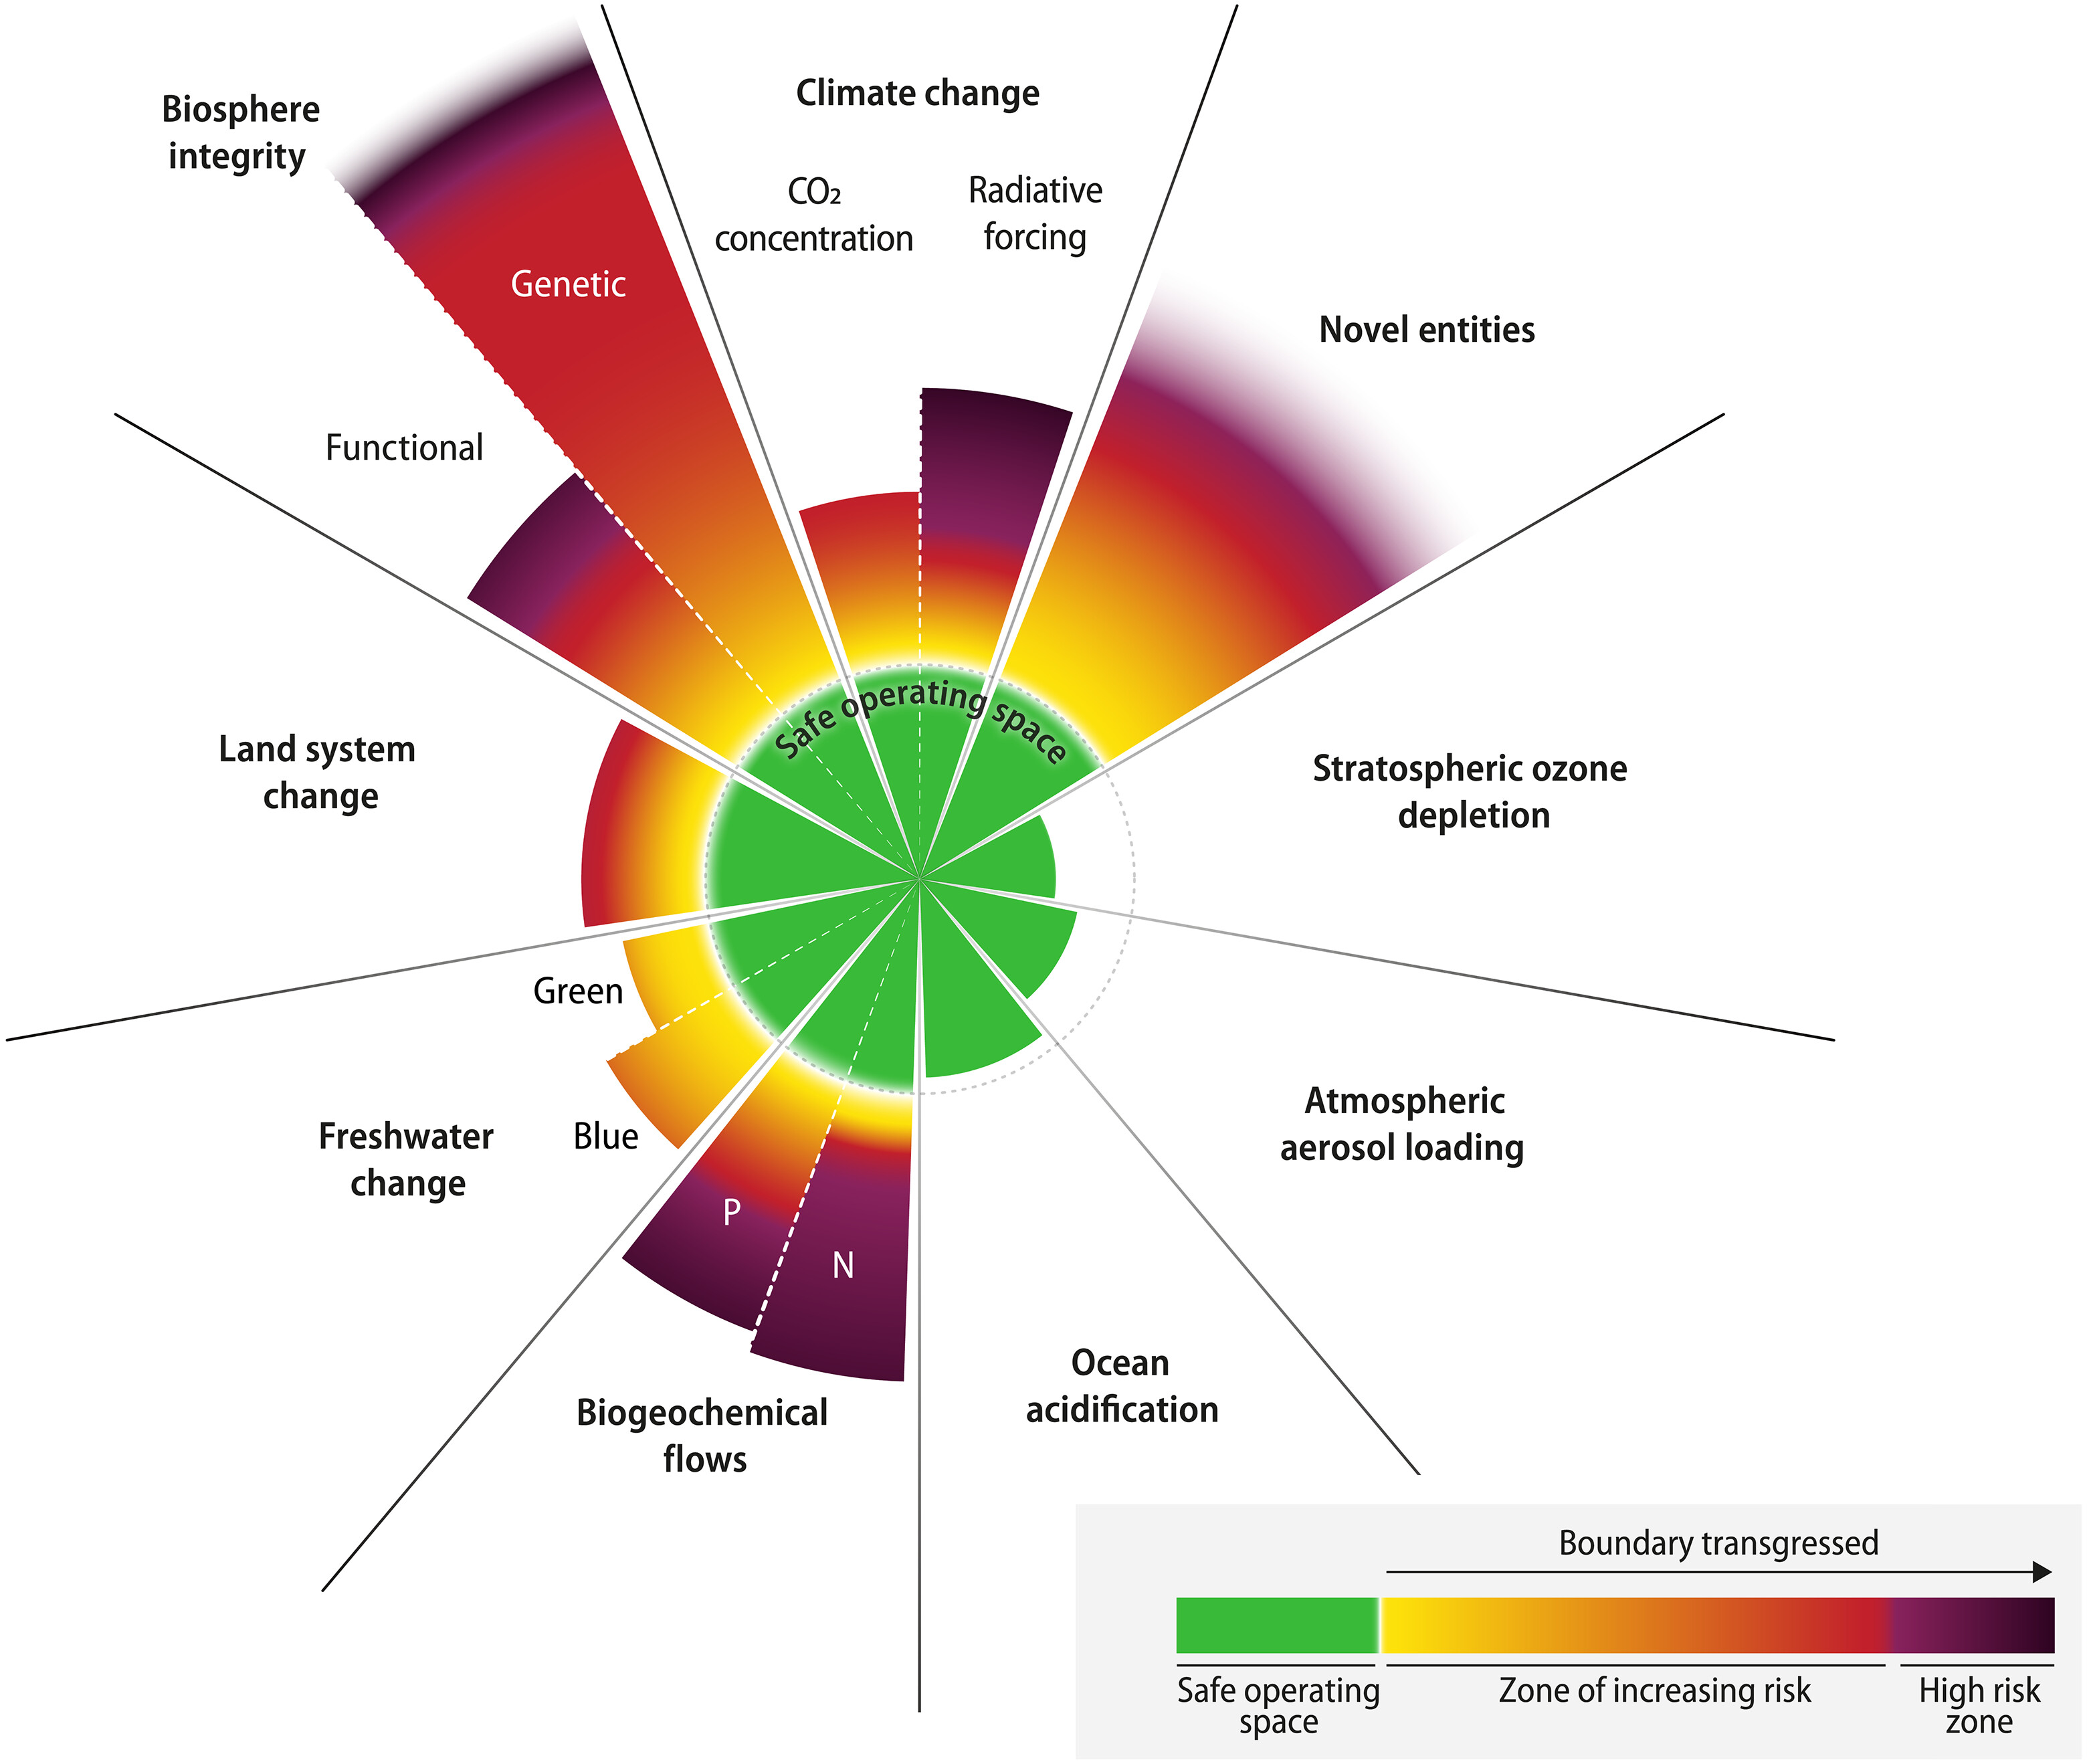
\includegraphics[width= .7\textwidth]{figures/intro/planetary_bounds.jpg}
	\caption{État actuel des variables de contrôle pour les neuf limites planétaires, à partir de \cite{richardson_earth_2023}}
\end{figure}

Parmi ces limites planétaires, l'intégrité de la biosphère a progressivement suscité un intérêt particulier, de même que son interaction avec d'autres limites, telles que le changement climatique, ou des entités nouvelles (par exemple, les polluants organiques synthétiques, les matières radioactives, la pollution microplastique...). Créé en 2012, le Groupe Interdisciplinaire sur la Biodiversité et les Services Ecosystémiques (IPBES\footnote{Interdisciplinary Panel on Biodiversity and Ecosystem Services}) a tiré la sonnette d'alarme sur l'état de la « nature » à l'échelle mondiale. Son président, Sir Robert Watson, l'a clairement exprimé\footnote{Voir le \href{https://www.ipbes.net/news/Media-Release-Global-Assessment}{communiqué de presse du rapport 2019}} :

\begin{displayquote}
\textit{Les preuves accablantes du Rapport d'Evaluation Global de l'\cite{ipbes_2022_6417333}, provenant d'un large éventail de domaines de connaissances, présentent un tableau inquiétant [...]. La santé des écosystèmes dont nous et d'autres espèces dépendons se détériore plus rapidement que jamais. Nous sommes en train d'éroder les fondements de nos économies, de nos moyens de subsistance, de notre sécurité alimentaire, de notre santé et de notre qualité de vie dans le monde entier}\footnote{Traduit par l'auteur}
\end{displayquote}

La « nature » est un concept central dans le cadre de l'IPBES \citep{ipbes_2022_6417333} :

\begin{displayquote} 
\textit{La nature (également définie comme la nature vivante) [est] le monde non humain, y compris les caractéristiques coproduites, avec un accent particulier sur les organismes vivants, leur diversité, leurs interactions entre eux et avec leur environnement abiotique. Dans le cadre des sciences naturelles, la nature comprend, par exemple, toutes les dimensions de la biodiversité, les espèces, les génotypes, les populations, les écosystèmes, la biosphère, le fonctionnement des écosystèmes, les communautés, les biomes, les systèmes de maintien de la vie sur Terre et leurs processus écologiques, évolutifs et biogéochimiques associés, ainsi que la diversité bioculturelle. Dans le cadre de l'économie, il comprend des catégories telles que les ressources naturelles biotiques, le capital naturel et les actifs naturels. Dans le contexte plus large des sciences sociales et humaines et des sciences environnementales interdisciplinaires, il est fait référence à des catégories telles que le patrimoine naturel, l'environnement vivant ou le non-humain. Dans le contexte d'autres systèmes de connaissance, il comprend des catégories telles que « Terre mère » [...], « Pachamama » [...]}.
\hspace*{\fill} \small{ \cite{ipbes_2022_6417333}, p.14, voir aussi \cite{DIAZ20151} }
\end{displayquote}

La nature, telle qu'elle est définie dans cette approche, est un objet très vaste et complexe. Elle se définit à travers des différences ontologiques et épistémiques (vivant et non-vivant), différents types d'interactions, à diverses échelles (génotypes v. écosystèmes), à différents types de processus (biologiques v. écologiques), et à travers différents champs d'investigation (sciences naturelles v. sciences sociales). Dans cette thèse, j'étudie plus spécifiquement la « biodiversité », qui se concentre sur la variabilité des organismes vivants. Bien qu'il s'agisse d'un concept ambigu, la biodiversité tend à mettre l'accent sur les organismes vivants, en relation avec leur environnement matériel, biotique et abiotique (par opposition à l'étude de l'environnement non vivant) et sur son rôle essentiel parmi les autres composantes du système terrestre.

Le rapport de l'\cite{ipbes_2022_6417333} documente les changements drastiques que subit la biosphère et examine ces changements dans une optique anthropocentrique, c'est-à-dire en médiatisant les changements susmentionnés par les contributions multiples et diverses que la nature et la biodiversité apportent à l'homme. Il souligne l'impact de leur perturbation sur la vie humaine et met en évidence le rôle des facteurs anthropogéniques (c'est-à-dire d'origine humaine) dans la perturbation de la nature et de la biodiversité. 
 
Ce rapport fixe différents objectifs à la recherche scientifique. Le premier objectif est d'expliquer les mécanismes de rétroaction : comment la vie de l'humanité influence-t-elle la biodiversité ? En réponse, comment la biodiversité influe-t-elle sur la vie de l'humanité ? Cet objectif implique, d'une part, de comprendre les causes et de mesurer les facteurs anthropiques directs et indirects de changement dans la nature et la biodiversité et, d'autre part, de comprendre les canaux et les échelles par lesquels la nature et la biodiversité contribuent aux moyens de subsistance de l'homme, ainsi que de mesurer ces contributions. Par conséquent, l'étude de la disparition de la nature et des possibilités d'y remédier nécessite une perspective intégrée, qui associe les sciences naturelles aux sciences sociales, par le biais de cadres tels que les systèmes socio-écologiques \citep{Ostrom2009} ou l'économie environnementale et écologique \citep{daly_ecological_2007}. 
\\
Le deuxième objectif est de fournir un cadre pour évaluer l'opportunité, la faisabilité et les moyens de mise en œuvre des voies collectives qui permettraient de remédier à la crise à laquelle la nature est confrontée. D'une certaine manière, il s'agit de concevoir et de mettre en œuvre des voies politiques vers des avenirs durables, c'est-à-dire de trouver des voies ou des méthodes d'action définies choisies parmi des alternatives, aux niveaux individuel, collectif ou gouvernemental, pour parvenir à des états futurs du monde qui restent dans un espace de fonctionnement sûr en ce qui concerne les limites planétaires \citep{rockstrom2009safe,steffen_2015_planetary}.

Dans cette thèse, j'aborde ces deux objectifs en utilisant un cadre issu de l'économie et de l'écologie. Une première version des questions de recherche que cette thèse vise à résoudre est la suivante : 

\begin{enumerate}
\item Quelles sont les relations de rétroaction entre la biodiversité et les facteurs anthropogéniques de son déclin ?
\item Quels sont les mécanismes sous-jacents auxquels les politiques doivent s'attaquer pour remédier à ce déclin ?
\item Comment les approches économiques et écologiques intégrées peuvent-elles être utilisées et affinées pour analyser, informer et concevoir des politiques publiques? 
\end{enumerate}

Afin d'affiner ces questions, je commence par définir le concept de biodiversité, à travers ses évaluations en sciences naturelles et sociales, et je souligne les tendances actuelles de sa disparition.

\phantomsection
\addcontentsline{toc}{section}{Emergence et définition de la biodiversité comme concept écologique}
\subsection*{Emergence et définition de la biodiversité comme concept écologique }


La biodiversité est apparue en tant que concept dans les années 1980, parallèlement à l'émergence de la « biologie de la conservation », une branche de la biologie qui s'intéresse à la protection de la « diversité biologique » \citep{soule_what_1985}, en réponse à l'accélération de la disparition des espèces. La position morale de la biologie de la conservation est que les espèces doivent être protégées pour elles-mêmes \citep{soule_conservation_1986}, elles ont une valeur intrinsèque. 
Le concept de biodiversité s'inscrit donc dans un jugement éthique et un appel à l'action. Dans le sillage de la conférence des Nations unies sur l'environnement et le développement qui s'est tenue à Rio en 1992, la \href{https://www.cbd.int/}{Convention sur la diversité biologique} s'est imposée comme un traité international visant à sauvegarder la biodiversité. Ce faisant, elle a fourni une définition internationalement reconnue :

\begin{displayquote}
\textit{La « diversité biologique » désigne la variabilité des organismes vivants de toute origine y compris, entre autres, les écosystèmes terrestres, marins et autres écosystèmes aquatiques et les complexes écologiques dont ils font partie ; cela comprend la diversité au sein des espèces et entre espèces ainsi que celle des écosystèmes.}\\
\hspace*{\fill} \small{\href{https://www.cbd.int/convention/articles/default.shtml?a=cbd-02}{Article 2 de la Convention sur la Diversité Biologique}}\footnote{Traduit par l'auteur}
\end{displayquote}

Cette définition met en évidence un élément clé de différenciation par rapport à d'autres parties de la nature, à savoir la nature vivante des objets étudiés. Par rapport aux facteurs abiotiques, la diversité biologique se caractérise par une croissance, une reproduction et un métabolisme intrinsèques (au niveau de l'individu et de la population), ainsi que par une évolution (au niveau de la génétique et de l'espèce). En outre, ces taux de changement dans le temps sont commensurables avec l'expérience humaine, et la plupart des processus (par exemple, la reproduction, l'effondrement ou la reconstitution des populations, l'évolution génétique) peuvent être observés au cours d'une vie humaine, par opposition à l'échelle temporelle géologique. 

Comme le soulignent \cite{VanDyke2008} et \cite{mouysset_diversity_2023}, la définition de la biodiversité est difficile, car elle recouvre des dimensions éthiques, conceptuelles et de mesure. La biodiversité peut être considérée comme « une qualité intrinsèque et sans mesure des systèmes naturels qui devrait être préservée pour elle-même » \citep{VanDyke2008, mouysset_diversity_2023}\footnote{Traduction de l'auteur}, mais elle se réfère également à des caractéristiques mesurables.
%
Cette définition implique différentes échelles d'un point de vue hiérarchique, au niveau génétique, au niveau de l'espèce, de la communauté et de l'écosystème (défini comme l'interaction des communautés et de leur environnement abiotique). Ces niveaux impliquent différentes formes de mesure, notamment la distribution des gènes, l'abondance des espèces (le nombre d'individus dans une population, à un moment et à un endroit donnés), la richesse des espèces (le nombre d'espèces différentes, à un moment et à un endroit donnés) au sein des communautés, entre les communautés et à des échelles plus grandes (les diversités alpha, bêta et gamma), ainsi que les variations des facteurs abiotiques qui forment les écosystèmes, tels que la température, l'humidité, la qualité de l'eau, la qualité du sol, etc. 
Elle comprend également différents types de diversité : la diversité structurelle (par exemple, les couches de la canopée dans les forêts, le sex-ratio dans les populations animales), la diversité de composition (la variété et l'abondance des espèces au sein d'une communauté) et la diversité fonctionnelle (la variété des processus environnementaux réalisés par les organismes vivants dans une zone donnée, par exemple la séquestration du carbone, le cycle des nutriments ou la dispersion des graines, voir \cite{loreau_biodiversity_2002}).

\begin{figure}[h]
	\centering
	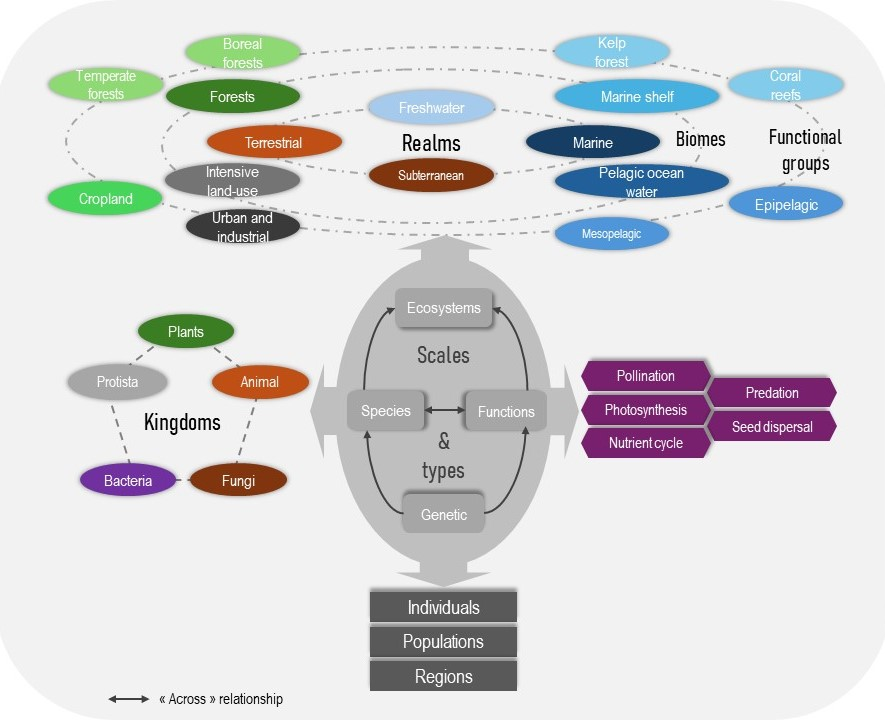
\includegraphics[width =.8\textwidth]{figures/intro/biodiv_illustration.jpg}
	\caption{ La biodiversité : un concept multiforme à travers échelles et types}
	\label{fig:intro_biod_french}
\end{figure}

\cite{mouysset_diversity_2023} souligne la difficulté d'articuler la définition avec les niveaux communs de l'analyse scientifique, par exemple génétique, taxonomique et écosystémique, car le niveau de biodiversité peut se situer entre les deux : « les populations peuvent être considérées d'un point de vue génétique et taxonomique, ou les communautés qui se situent entre les niveaux taxonomique et écosystémique ». En outre, la diversité structurelle et compositionnelle pouvant être considérées comme les sources de la diversité fonctionnelle, il peut être difficile de travailler avec les différentes classes de diversité en raison de leur colinéarité. 

Les multiples dimensions de la biodiversité mettent en évidence plusieurs de ses caractéristiques essentielles. Tout d'abord, il est impossible de mesurer la biodiversité à l'aide d'un seul indicateur. L'étude de la biodiversité nécessite de multiples indicateurs pour évaluer de manière intégrée l'évolution de la biodiversité, à toutes les échelles et pour tous les types de diversité. L'émergence du concept répond à un désir de protéger la biodiversité pour son propre bien, mais aussi pour celui de l'humanité. 

\phantomsection
\addcontentsline{toc}{section}{Les Contributions de la Nature  aux Populations : logiques de conservation de la biodiversité}
\subsection*{Les Contributions de la Nature aux Populations : logiques de conservation de la biodiversité}

D'abord descriptives, les fonctions des écosystèmes ont été de plus en plus considérées d'un point de vue humain à partir des années 1970 \citep{hueting1969functions, schumacher1973small}, évoluant vers le concept de services écosystémiques \citep{ehrlich1981extinction} pour illustrer les conséquences de la perte de biodiversité \citep{gomez_history_2010}. Cette évolution a marqué le passage d'une valeur intrinsèque à une valeur anthropocentrique (c'est-à-dire donnée par l'homme) \citep{mouysset_diversity_2023}, reconnaissant les valeurs instrumentales et relationnelles de la biodiversité - servir les objectifs des humains et favoriser des relations significatives avec les autres et l'environnement. Progressivement, la biodiversité a dû être protégée pour son rôle dans le maintien de la vie humaine.

Le concept a fait son chemin dans la recherche universitaire, et lorsque \cite{Costanza1997} a quantifié la valeur du capital naturel et des services écosystémiques au stupéfiant montant de 33 trillions \$USD, soit environ 30\% du PIB mondial de 2020, le concept est entré dans l'arène politique. En 2005, le Millenium Ecosystem Assessment \citep{MEA2005} a placé les services écosystémiques au centre de l'agenda politique : elle a souligné une valeur anthropocentrique des services écosystémiques, mais a établi une dépendance des sociétés humaines aux services écosystémiques, et plus loin, au fonctionnement de l'écosystème. À cet égard, le Millenium Ecosystem Assessment \citep{MEA2005} a marqué un tournant dans la sauvegarde de la biodiversité par le biais d'un paradigme de soutenabilité forte (voir encadré 1), et a déclenché l'opérationnalisation du concept dans les politiques à grande échelle (ce que je développerai plus loin). Le cadre des services écosystémiques a été divisé en 4 catégories, liées au type spécifique de services contribuant au « bien-être humain » : les services de soutien (par exemple, les services permettant à d'autres services écosystémiques d'être présents, y compris le cycle des nutriments et la production primaire) et les services de régulation (« avantages obtenus par la régulation des processus écosystémiques », par exemple la pollinisation, la décomposition des déchets, la gestion de l'eau, etc.) ; les services culturels (« les avantages non matériels que les gens tirent des écosystèmes par l'enrichissement spirituel, le développement cognitif ») et les services d'approvisionnement (« tous les produits tirés des écosystèmes »,\cite{MEA2005}, p.54)

\begin{figure}[h]
	\centering
	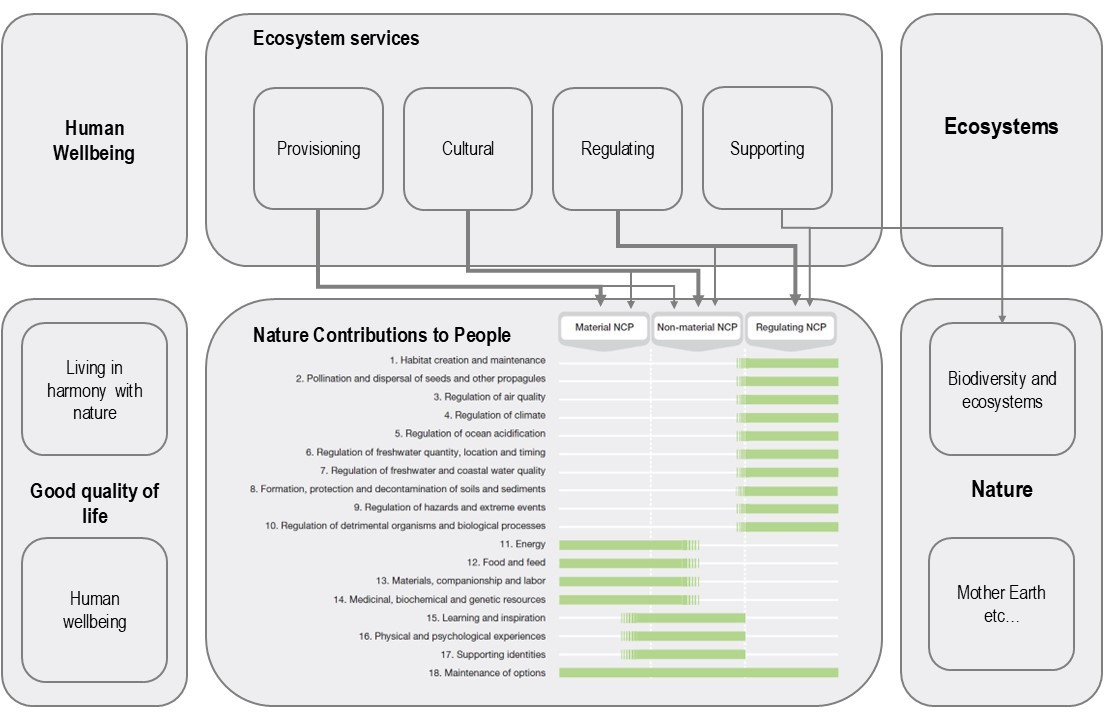
\includegraphics[width = \textwidth]{figures/intro/NCPs2.jpg}
	\caption{Description des 18 Contributions de la Nature aux Populations et du lien entre le cadre des CNP \citep{ipbes_2022_6417333} et le cadre des services écosystémiques \citep{millennium2005ecosystems}}
	\subcaption*{Adapté depuis \cite{diaz_2018} et \cite{ipbes_2022_6417333}}
\end{figure}

Récemment, l'IPBES est passée à un nouveau cadre conceptuel mettant en évidence les contributions de la nature aux populations (CNP) \citep{DIAZ20151}, définies comme « toutes les contributions, positives et négatives, de la nature vivante [...] à la qualité de vie des populations » \citep{diaz_2018}. Ce cadre sous-tend trois types de contributions aux personnes : les contributions matérielles aux personnes (flux de la nature vers les personnes généralement consommés pour « faire fonctionner une société ou une entreprise » \cite{ipbes_2022_6417333}, p.16), les contributions non matérielles (par exemple, les effets de la nature sur « les aspects subjectifs et psychologiques qui sous-tendent la qualité de vie des populations ») et les contributions régulatrices (par exemple, « les aspects fonctionnels et structurels des organismes et des écosystèmes qui modifient les conditions environnementales vécues par les personnes et/ou régulent la génération de contributions matérielles et non matérielles »). Ce cadre met en évidence le fait que les contributions de la nature à l'homme peuvent être positives ou négatives et dépendent de la définition spatiale et temporelle de la contribution, puisqu'une entité donnée peut être à la fois la source de contributions positives et négatives : par exemple, les forêts favorisent l'habitat, mais risquent également de mettre en danger les personnes en cas d'incendies de forêt. En outre, elle offre une vision plus globale que les services écosystémiques, car elle englobe des perspectives allant de la biodiversité en tant que capital naturel utilisé dans une fonction de production écologique (voir \cite{polasky_integrating_2009} pour une revue), ainsi que des perspectives où la biodiversité a une agence et est liée par des obligations de soins réciproques envers les humains \citep{descola}. 

Une correspondance à multiples facettes entre les différentes composantes et dimensions de la biodiversité et ses contributions à l'homme est à la base des moyens de subsistance de l'homme. Le déclin mondial de la biodiversité menace les CNP.

\clearpage
\begin{tcolorbox}[breakable,  
colback=verylightgray, 
colframe=gray!75!black, 
title= {Box 1 - Soutenabilité Faible et Forte},
fontupper=\small]

\par % This \par ensures spacing before the text starts
\justifying % Start justified text

En 1987, la publication du rapport Brundtland \citep{brundtland} a donné une définition large du développement durable : 

\begin{displayquote}
\textit{Par essence, le développement durable est un processus de changement dans lequel l'exploitation des ressources, la direction des investissements, l'orientation du développement technologique et les changements institutionnels sont tous en harmonie et améliorent le potentiel actuel et futur de satisfaction des besoins et des aspirations de l'humanité}\footnote{Traduit par l'auteur}\\
\hspace*{\fill}\small{\cite{brundtland}, p.43}
\end{displayquote}

La mise en œuvre du développement durable est restée une question ouverte. En économie, une « perspective de durabilité faible », inaugurée par les travaux de \cite{hartwick_intergenerational_1977} et \cite{solow_intergenerational_1986} sur les ressources épuisables, suggérait que « le maintien d'un stock de capital non décroissant, qui pourrait être mis en pratique en investissant dans le capital manufacturé toutes les rentes dérivées de l'exploitation des ressources naturelles non renouvelables »\footnote{Traduit par l'auteur} \citep{gomez_history_2010} était suffisant pour maintenir la consommation au fil du temps. Dans cette approche, le capital naturel pouvait être intégralement remplacé par le capital humain. D'autre part, l'approche de la « durabilité forte » prône la complémentarité, plutôt que la substituabilité, des ressources naturelles \citep{costanza_daly}, reconnaissant ainsi la dépendance des humains à l'égard des écosystèmes.
\end{tcolorbox}

\phantomsection
\addcontentsline{toc}{section}{Déclin de la biodiversité : tendances et facteurs}
\subsection*{Déclin de la biodiversité : tendances et facteurs}

Les mesures de la biodiversité diminuent à toutes les échelles d'analyse. Les conditions structurelles des écosystèmes, la composition des communautés écologiques et les populations d'espèces ont connu des changements spectaculaires.
La part des habitats sauvages protégés et inchangés s'est effondrée sur terre et en mer \citep{watson_2016_catastrophic, jones_2018_location} pour atteindre 23\% et 12\% de l'espace, respectivement. Au niveau des communautés, la part de la biodiversité initialement présente tombe en dessous de 90 \% dans tous les biomes, \citep{Hill311787} et les communautés locales deviennent de plus en plus semblables \citep{mckinney_1999_biotic}, sous l'effet de l'augmentation de l'étendue des espèces exotiques envahissantes animales et végétales, en hausse de 13 \% par décennie \citep{seebens_no_2017}. A\` ce jour, la richesse des espèces mondiales est menacée par une extinction massive, car le taux mondial d'extinction des espèces est au moins dix fois plus élevé que le taux moyen des 10 derniers millions d'années et s'accélère \citep{barnosky_has_2011, ceballos_accelerated_2015}. En moyenne, 25 \% des espèces sont actuellement menacées d'extinction à l'échelle mondiale dans un large éventail d'espèces végétales et animales, sur terre et en mer \citep{IUCN_redlist_2024}. En utilisant des méthodes fondées sur l'habitat, \cite{Hoskins309377}\footnote{La liste rouge de l'UICN utilise des comptes détaillés pour les espèces, dans une approche ascendante, afin d'analyser le risque d'extinction des espèces. Une approche descendante, qui s'appuie sur l'évolution de l'habitat disponible et la relation espèce-zone, utilise les changements dans l'utilisation des terres pour prévoir l'extinction des espèces de manière plus globale. \citep{Diamond1972BiogeographicKE}} constatent que des centaines de milliers d'espèces végétales et animales sont menacées et rembourseront la \textit{dette d'extinction} causée par les changements anthropogéniques de leurs habitats : seulement 92.1\% des espèces de vertébrés terrestres, 91,6\% des invertébrés terrestres et 90,7\% des plantes terrestres disposent d'un habitat suffisant pour subsister. Ces résultats suggèrent qu'environ un demi-million d'espèces animales et végétales terrestres - dont plus de 3 000 vertébrés et plus de 40 000 plantes - sont condamnées à s'éteindre, à moins que leurs habitats ne s'améliorent à temps pour l'empêcher \citep{ipbes_2022_6417333}.

Les facteurs de déclin de la biodiversité sont d'origine anthropique. Ils peuvent être classés en deux catégories : les facteurs \textit{directs}, qui découlent directement des actions humaines, comme le changement d'utilisation des terres, le changement climatique anthropique, la surexploitation, et les facteurs \textit{indirects}, qui peuvent être considérés comme la cause première des facteurs directs, comme les changements dans les systèmes de valeurs qui sous-tendent les utilisations de la nature (\cite{ipbes_2022_6417333} p. 55), la démographie (urbanisation et migration), la technologie, l'économie (transitions sectorielles, expansion du commerce) et la gouvernance (y compris les systèmes de risque pour l'accès aux ressources).

Une synthèse des sciences naturelles réalisée par l'\cite{ipbes_2022_6417333} souligne le rôle des principaux facteurs à l'échelle mondiale et dans tous les biomes (voir figure \ref{fig:intro_impacts_french}).
Il montre que le changement d'utilisation des terres et des mers, c'est à dire la perte, la fragmentation, et la dégradation de  l'habitat\footnote{La perte d'habitat est sans aucun doute le principal moteur du déclin de la biodiversité terrestre. Les effets de la fragmentation sur la biodiversité sont très controversés. D'un point de vue théorique, des modèles ont été développés pour étudier l'évolution des populations et des communautés dans l'espace et le temps, par exemple les modèles de métapopulation et de métacommunauté. Les connaissances théoriques soulignent que la fragmentation de l'habitat augmente le risque d'extinction et réduit la probabilité de colonisation, ce qui se traduit par une baisse de la survie et de la diversité \citep{adler_persistence_1994,hill_habitat_1999, thompson_loss_2017}. À l'échelle communautaire, l'augmentation de la diversité entre les communautés (par exemple, la diversité bêta) peut résulter des différentes exigences des espèces en matière de ressources et de la plus grande étendue spatiale, qui englobe donc une plus grande hétérogénéité environnementale, résultant de la fragmentation \citep{lasky_reserve_2013, chisholm_species_2018}. Toutefois, ces effets s'atténuent à mesure que la perte d'habitat diminue.   Au niveau empirique, l'effet de la fragmentation est très discuté. Selon \cite{fahrig_ecological_2017}, il n'existe aucune preuve empirique qu'un groupe de petites parcelles d'habitat a généralement une valeur écologique inférieure à celle de grandes parcelles de la même superficie totale. Des éléments montrent toutefois que la fragmentation ne réduit pas la connectivité des habitats, car la connectivité fonctionnelle est améliorée (par exemple, les espèces sont en contact avec un plus grand nombre de parcelles de ressources différentes, ce qui améliore le fonctionnement global des écosystèmes). Le débat entre \cite{fletcher_is_2018} et \cite{fahrig_habitat_2019} porte sur les critiques fondées sur la capacité des modèles statistiques à englober l'effet de la fragmentation en cas de perte d'habitat \citep{ruffell_accounting_2016}. En outre, il reflète la difficulté de l'écologie paysagère, car différents mécanismes à travers les échelles, par exemple la parcelle, le paysage et la région d'étude, et des mesures, telles que la taille de la parcelle, l'isolement de la parcelle (par exemple la distance entre les parcelles) et la distance au bord de la parcelle (par exemple la distance au bord à l'intérieur de la parcelle) interagissent avec des interactions non linéaires possibles.}
\%
L'exploitation directe de la faune et de la flore sauvages et la dégradation de l'habitat de la faune sont responsables de 30\% des impacts sur la biodiversité. L'exploitation directe de la faune et de la flore sauvage représente 23 \% des impacts. Le changement climatique, qui se traduit par des modifications des conditions biogéographiques et des changements d'habitat, a un impact sur les caractéristiques des espèces et l'évolution génétique, ce qui représente 14\% des impacts, et la pollution représente 14\% des impacts. Enfin, les espèces exotiques envahissantes représentent 11\%. Ces facteurs ont des impacts différents selon les écosystèmes et les biomes \citep{ipbes_2022_6417333}. 

\begin{figure}[h]
	\centering
	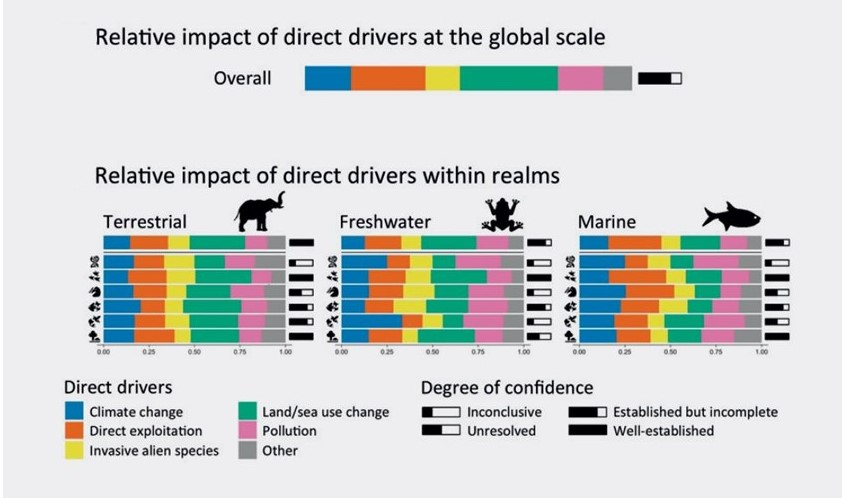
\includegraphics[width = .95 \textwidth]{figures/intro/intro_impactsfin.jpg}
	\caption{Effets aggrégés et par biômes des impacts des moteurs anthropogéniques directs du déclin de la biodiversité, adapté de  \cite{ipbes_2022_6417333}}
	\label{fig:intro_impacts_french}
\end{figure}

Sur terre, le changement d'usage des terres est le facteur le plus important (30,5\%), sous l'effet de la déforestation et de l'agriculture, suivi de l'exploitation directe (21\%).  Les forêts tropicales et subtropicales sèches et humides abritent la plus grande diversité biologique. Par exemple, elles abritent les 10 hotspots qui comptent le plus grand nombre de vertébrés \citep{mittermeier_global_2011}. Dans ces forêts, la perte et la dégradation de l'habitat sont les principaux facteurs de réduction de l'abondance et de la richesse des espèces \citep{newbold_global_2014}. L' exploitation forestière sélective légale et illégale détruit l'habitat \citep{hoare2022establishing, bousfield_2023_large} et est combinée à la chasse et au braconnage des espèces sauvages \citep{gallego_2020_combined}, générant entre 60 et 180 milliards \$ USD de revenus \citep{gfi_2017}\footnote{Le commerce illégal d'espèces sauvages représente entre 5 et 23 milliards \$USD, tandis que l'exploitation forestière illégale représente entre 52 et 157 milliards \$USD}. 

Pour les espèces marines, la surexploitation est le principal moteur (29\%) \citep{ipbes_2022_6417333}. Avec 90 millions de tonnes de captures (et 141 milliards de dollars) en 2020 \citep{fao_2022_state}, les stocks halieutiques se situant à des niveaux biologiquement durables ont diminué pour atteindre 64,6\% en 2019, contre 90\% en 1974\footnote{Dans ce calcul, tous les stocks halieutiques sont pris en compte de la même manière, indépendamment de leur abondance ou de leurs captures}, sous l'effet de la surpêche dans le Pacifique Sud-Est et dans les mers Méditerranée et Noire. Néanmoins, la pêche illicite, non déclarée et non réglementée (INN) constitue une menace pour les pêcheries.  Selon des estimations datant d'il y a 15 ans \citep{agnew_estimating_2009} , elle représenterait entre 11 et 26 millions de tonnes de poisson pour une valeur de 10 à 23 milliards de dollars américains. 

En outre, le changement climatique anthropique entraîne des perturbations des écosystèmes sur terre \citep{burrell_anthropogenic_2020, conradi_reassessment_2024} et en mer \citep{gomes_marine_2024}, par le biais de changements dans divers canaux , y compris l'adéquation des habitats et les perturbations du réseau trophique. Sur terre, par exemple, les forêts, bois et maquis méditerranéens, qui couvrent 4 millions de km$^2$, sont des zones d'une diversité exceptionnellement élevée \citep{Mooney2001, blondel_2010}, menacées par l'expansion urbaine et l'augmentation du risque d'incendie de forêt.   La fréquence et la gravité des incendies de forêt devraient augmenter avec le réchauffement climatique \citep{Dupuy2019ClimateCI}, entraînant d'importants coûts directs et indirects pour la société , notamment la destruction d'infrastructures et des perturbations de l'activité économique \citep{wang_economic_2021}, les problèmes de santé liés à lafumée \citep{burke_wildfire_2023, heft-neal_behavior_2023}, la perturbation des caractéristiques structurelles des écosystèmes \citep{Ayars2023} et la menace pour la diversité biologique \citep{Wintle2020}.

\phantomsection
\addcontentsline{toc}{section}{Défis économiques des facteurs anthropogéniques du déclin de la biodiversité}
\subsection*{Défis économiques des facteurs anthropogéniques du déclin de la biodiversité}


La perte d'habitat et la surexploitation présentent des défis à la fois communs et différenciés.   Une cause commune identifiable est le coût d'opportunité élevé de la préservation de l'habitat ou de l'existence d'une espèce, en présence d'autres alternatives économiques pour la terre et le temps, ainsi que de contraintes financières. En outre, la perte d'habitat et la surexploitation partagent un aspect dynamique temporel, où les actions immédiates ont des conséquences durables, voire irréversibles.

La perte et la fragmentation de l'habitat dans les écosystèmes terrestres posent des problèmes spécifiques. Les forêts, par exemple, ont des usages multiples (ou CNP) pour différents agents : les bûcherons tirent profit du bois, certains défrichent les terres pour l'agriculture, les randonneurs recherchent des paysages vierges et les défenseurs de l'environnement visent à rétablir les cycles naturels. Les forêts ont également une valeur spirituelle et culturelle. Ces différents usages rentrent donc en conflit. Par exemple, la déforestation et l'urbanisation détruisent à la fois l'habitat et les terres sacrées, mais créent une valeur économique mesurée \citep{giglio_economics_2024}, tandis que la prévention des incendies de forêt peut endommager l'habitat des espèces sauvages \citep{bradshaw2018}. Les espèces peuvent également avoir des impacts mixtes ; les cerfs, par exemple, sont appréciés à faible densité mais causent des dommages à des densités plus élevées \citep{putman_identifying_2011}. Le changement climatique aggrave la perte d'habitat en modifiant la distribution des habitats et en augmentant les menaces telles que les incendies de forêt \citep{Dupuy2019ClimateCI,wasserman_climate_2023}.
    Une deuxième caractéristique essentielle pour mettre fin à la fragmentation des habitats est la prise en compte de l'ensemble des interdépendances, des retombées écologiques et des externalités économiques qui sous-tendent la dimension spatiale. La configuration de l'espace et le mouvement des espèces sont, au moins en partie, le résultat d'une décision économique. Le maintien de la connectivité des habitats passe par l'identification des parcelles et des chemins à conserver ou à restaurer qui y contribuent le plus, sous forme de corridors, d'écoducs ou de tremplins \citep{Turner2005, Turner2011}. La valeur des parcelles et des chemins pour la connectivité est intrinsèquement liée à leur environnement : au même endroit géographique, une parcelle a une valeur différente pour l'habitat de la biodiversité si elle est connectée à d'autres, ou si elle est isolée (voir encadré 2). Lorsque les chemins échappent au contrôle de l'homme, les parcelles ont une importance différente en fonction de leur emplacement, et lorsque l'emplacement des parcelles est fixe, l'étendue des chemins et leur emplacement sont primordiaux.
\\
Troisièmement, lorsque des actions et des utilisations multiples structurent des éléments connectés des écosystèmes (par exemple, différentes étendues de terre ou différentes échelles de biodiversité), elles entraînent des retombées spatiales, c'est-à-dire des conséquences qui vont au-delà de leurs effets \textit{in situ}, avec des répercussions dnas la durée. Lorsque ces retombées ne sont pas prises en compte par les agents qui les génèrent, elles peuvent être appelées « externalités spatiales dynamiques » \citep{sanchirico_bioeconomics_1999, costello_optimal_2008, costello_private_2017}. Étant donné que l'arrêt de la perte et de la fragmentation des habitats implique la conservation de parcelles de terre, les parties voisines peuvent très bien bénéficier (ou souffrir) d'un plus grand nombre d'espèces sauvages et de (dis-)services écosystémiques sur leur propriété, au fil du temps. Comme les agents réagissent aux profils d'action des autres, ils adoptent un comportement stratégique, à la fois dans l'espace et dans le temps. Ces externalités peuvent déclencher des problèmes spécifiques de « cercle vicieux » \citep{costello_private_2017} : lorsque les parties voisines d'un décideur qui entreprend la conservation, ou la réduction des risques, ne se rendent pas la pareille alors qu'elles bénéficient des retombées, un cercle vicieux de moindre action est déclenché. Inversement, lorsque les retombées écologiques sont positives, cela peut conduire tout le monde à utiliser une ressource à des niveaux non durables, même en présence de droits bien définis, en l'absence d'autres mécanismes \citep{janmaat_sharing_2005,kaffine_unitization_2010}.  Par conséquent, la fragmentation de l'habitat et la surexploitation sont liées par la connectivité spatiale. 
\\
Quatrièmement, arrêter la perte et la fragmentation des habitats implique de coordonner de nombreux acteurs en vue d'accroître la superficie et la connectivité des habitats, tout en tenant compte des coûts et des avantages associés, ainsi que des différents intérêts.
Dans certains cas, les contraintes financières, l'ampleur des coûts associés à l'augmentation de la connectivité des habitats et la difficulté de la coordination justifient une politique publique dans laquelle un planificateur central entreprend l'action \citep{Mouysset2012}. D'autre part, il existe des mécanismes permettant de décentraliser une planification spatiale efficace, qui peuvent être efficaces lorsque les coûts de coopération sont limités \citep{costello_private_2017, bareille_agglomeration_2023}. 

Pour mettre un terme à la surexploitation, il faut comprendre et traiter ses motivations. La surexploitation (ou le sous-contrôle, pour les espèces nuisibles) résulte d'un déséquilibre entre l'appropriation et l'utilisation des contributions de la nature aux populations (tant positives que négatives) et le niveau et la répartition socialement souhaitables de ces contributions, ainsi que du comportement stratégique non coordonné des agents. La nature commune de la plupart des ressources naturelles \citep{Gordon1954, smith_models_1969} a longtemps été identifiée comme l'une des principales raisons de leur disparition : de nombreux événements ont montré eux aussi des dynamiques de cercles vicieux, de tragédie des communs \citep{hardin_tragedy_1968}, où l'absence de droits de propriété sûrs a accéléré la surexploitation et le déclin des populations. Cette question est depuis longtemps au centre de l'attention, et les mécanismes reposant sur l'attribution de droits de propriété ont fait l'objet d'études approfondies \citep{libecap_tragedy_2009, costello_partial_2015, isaksen_tragedy_2019}.

\clearpage
\begin{tcolorbox}[breakable, 
colback =verylightgray, 
colframe=gray!75!black,
title={Encadré 2 - Habitat : perte, fragmentation et connectivité},
fontupper=\small]
\par 
\justifying

La perte d'habitat correspond à la perte de zones présentant des conditions environnementales adéquates pour la survie et le développement des espèces. À surface d'habitat constante, la fragmentation se traduit par une augmentation du nombre de parcelles et une diminution de la taille moyenne de chaque parcelle, comme le montre la figure \ref{fig:connectivity_intro_french}. 

La connectivité du paysage est définie par rapport à la fragmentation. Elle mesure « le degré auquel le paysage facilite ou entrave le mouvement entre les parcelles de ressources » \citep{taylor_connectivity_1993}. 
Elle recouvre une dimension \textit{structurelle}, qui décrit les arrangements physiques entre les parcelles, et une dimension \textit{fonctionnelle}, qui met l'accent sur la capacité et la réalisation des mouvements des individus à travers le paysage. Les mesures de connectivité globale tiennent compte du rôle des parcelles et des chemins différenciés. Dans le panneau D de la figure \ref{fig:connectivity_intro}, les parcelles encerclées jouent un rôle déterminant dans le maintien de la connectivité. Les parcelles d'habitat 1 et 2 ont le même nombre de parcelles connectées. Cependant, la parcelle 1 maintient la connexion entre les parcelles d'habitat situées à l'est et à l'ouest du paysage et est reliée à des parcelles fortement connectées. La suppression des parcelles d'habitat 1 et 2 aurait des conséquences plus importantes sur l'habitat que la suppression d'autres parcelles de taille identique. De même, la suppression du chemin en pointillé (en bas à gauche du panneau D) isolerait la parcelle 3, tandis que la suppression du chemin en pointillé ne laisserait pas la parcelle 4 isolée. Par conséquent, les chemins et les îlots ont des impacts différents sur la connectivité, en fonction des îlots et des chemins environnants.

\begin{center}
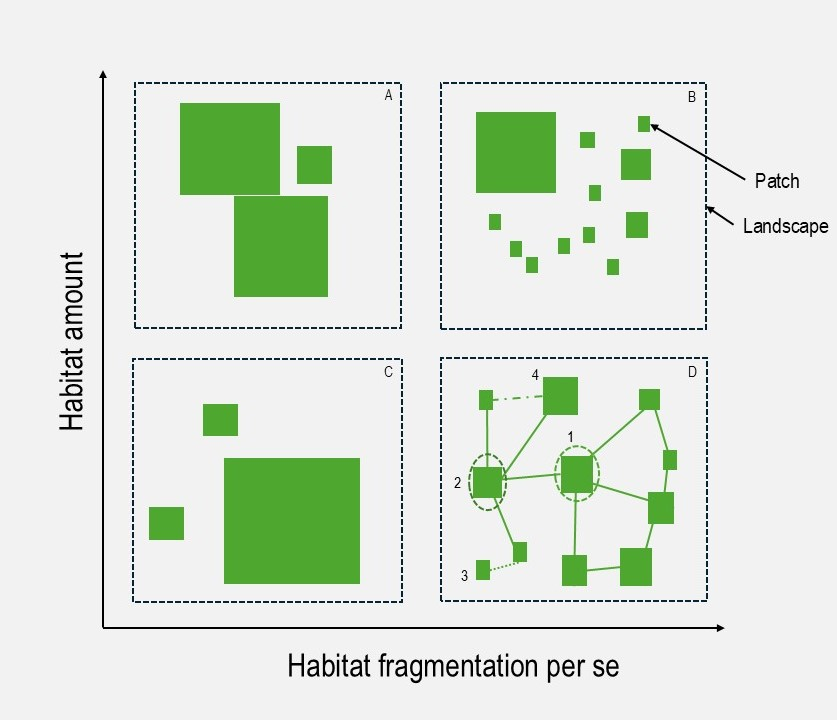
\includegraphics[width = .8\textwidth]{figures/intro/fragmentation.jpg}
\captionof{figure}{Illustration des effets de la perte d'habitat et de la fragmentation , adapté de \cite{fahrig_habitat_2019}, ainsi que des effets de la connectivité}
\label{fig:connectivity_intro_french}
\end{center}
\end{tcolorbox}

Toutefois, si les droits de propriété peuvent être attribués, il est notoirement difficile de les faire respecter dans les régions où les fonctions régaliennes sont contestées: des droits \textit{de facto}, et non \textit{de jure} sont attribués et appliqués. Dans ce cas, la nature commune de la ressource peut ne pas être la principale préoccupation: les forces locales de concentration du marché peuvent l'emporter sur les forces de surexploitation, même en présence d'une certaine forme d'accès libre \citep{damania_economics_2007}.  Dans le monde entier, le braconnage et le commerce d'espèces sauvages sont généralement le fait de groupes criminels organisés et sont associés à différentes activités criminelles \citep{mozer_introduction_2023}.  Des marchés concentrés tendent à émerger et à caractériser les marchés des espèces sauvages, car la concurrence est entravée par des groupes criminels organisés violents. Dans ce cas, la gestion des ressources est stratégique et répond aux caractéristiques du marché (structure de la demande, prix des marchandises intermédiaires) et aux caractéristiques écologiques (distribution des espèces, taux de croissance biologique, capacité de charge\footnote{La notion de \textit{capacité de charge} est utilisée depuis le milieu du XXème siècle par les écologistes des populations (pour un historique de la notion, voir \cite{sayre_carrying_2008}) pour décrire la taille maximale de la population d'une espèce qu'un écosystème donné peut supporter à long terme})
À un extrême, une structure de marché monopolistique locale pour les produits de la faune sauvage peut émerger, en particulier dans le cas d'espèces endémiques (par exemple, indigènes et limitées à une zone). Un monopole peut être le meilleur ami des défenseurs de la nature \citep{solow_resources_1974, hannesson_note_1983}, en fonction des caractéristiques spécifiques du marché et des espèces, qui dépendent du contexte, car un monopole a intérêt à restreindre l'offre pour augmenter les prix, si les consommateurs ne réagissent pas trop (par exemple, en cas d'élasticité limitée de la demande). Un large éventail de structures de marché \citep{damania_economics_2007, hannesson_effects_1985} appliquées à des situations réelles a été étudié. Cependant, l'ensemble des interactions entre l'endémisme d'une espèce, le pouvoir de marché local, le coût de l'effort et l'accès aux marchés de consommation finale nécessite une analyse plus approfondie afin de clarifier l'impact de la structure du marché.

D'autres facteurs de surexploitation peuvent être trouvés dans les bénéfices importants attendus (par rapport à d'autres activités économiques locales) que certaines ressources naturelles peuvent supporter, la plupart du temps en raison de leur rareté (par exemple, l'absence de substitut économiquement viable), que ce soit aujourd'hui ou à l'avenir \citep{Kremer2000}.  Alors que les effets de la substitution de produits fabriqués par l'homme aux services écosystémiques perturbés commencent à faire l'objet d'études empiriques \citep{frank_economic_2024} et montrent à quel point les coûts peuvent être redoutables, l'effet de l'introduction de substituts aux produits de la faune sauvage braconnés illégalement peut être un exemple de substituabilité forte entre les actifs naturels et artificiels \citep{chen_economics_2017}. Comme des forces plus larges affectent la surexploitation, y compris la pauvreté, il est clair que le traitement de la surexploitation implique de généraliser le raisonnement portant sur  l'interaction d'une seule espèce avec le cadre institutionnel, comment l'avenir d'une espèce interagit avec la disponibilité des substituts, et comment la distribution des revenus provenant des récoltes durables peut favoriser une utilisation raisonnée de la ressource. 
	
Un large éventail de politiques a été mis en œuvre à différents niveaux organisationnels, afin d'enrayer, conjointement ou séparément, les facteurs identifiés de déclin de la biodiversité sur terre et en mer, avec plus ou moins de succès. 

\phantomsection
\addcontentsline{toc}{section}{Politiques publique de la biodiversité : du global au local}
\subsection*{Politiques publiques de la biodiversité : du global au local}
\par

Les cadres politiques internationaux successifs ont cherché à enrayer la perte de biodiversité en s'attaquant à ses facteurs de manière globale.    En 2022, la 15e conférence de la Convention des Nations unies sur la diversité biologique a lancé le \href{https://www.cbd.int/doc/c/e6d3/cd1d/daf663719a03902a9b116c34/cop-15-l-25-fr. pdf}{Keunming Montreal Global Biodiversity Framework (GBF)}, remplaçant le Plan stratégique pour la biodiversité 2011-2020 et les Objectifs d'Aichi après avoir échoué à atteindre ses objectifs\footnote{Parmi les 20 Objectifs d'Aichi, aucun n'a été atteint au niveau mondial en 2020, et seulement 6 ont été partiellement atteints , y compris l'identification et l'éradication des espèces envahissantes sur les îles, la désignation de 17\% des zones terrestres et des eaux intérieures et de 10\% des zones côtières et marines comme zones de conservation, la mise en œuvre d'instruments politiques et d'une stratégie et d'une planification nationales efficaces en matière de biodiversité, et l'augmentation du financement de la protection de la biodiversité.  Les raisons invoquées pour cet échec sont l'absence d'indicateurs clairs pour évaluer les objectifs, et l'absence d'obligation de rendre compte des progrès accomplis dans la réalisation des objectifs \citep{maron_setting_2021}}. Le GBF fixe quatre objectifs mondiaux pour 2050, avec 23 objectifs mesurables pour stopper la perte de biodiversité d'ici 2030. Ces objectifs comprennent le maintien de l'intégrité et de la connectivité des écosystèmes et la prévention des extinctions induites par l'homme (objectif A), l'utilisation durable de la biodiversité (objectif B), le partage équitable des avantages et des charges liés à la conservation (objectifs C et D)\footnote{Voir \href{https://www.cbd.int/doc/c/e6d3/cd1d/daf663719a03902a9b116c34/cop-15-l-25-fr.pdf}{Section G. Keunming Montreal Global Biodiversity Framework pour 2050}}. \href{https://www.cbd.int/gbf/targets/5}{Les objectifs } comprennent la restauration de 30\% des écosystèmes dégradés, la conservation de 30\% des zones terrestres et marines et la garantie de l'utilisation et de la gestion durables des espèces sauvages.
  
 
 D'autres traités internationaux, tels que la \href{https://cites.org/fra}{Convention sur le commerce international des espèces de faune et de flore sauvages menacées d'extinction (CITES)} établie en 1973, réglementent le commerce des espèces menacées d'extinction afin d'empêcher le commerce illégal des espèces sauvages\footnote{CITES compte 183 parties membres (pays), elle répertorie les espèces à travers des «annexes», avec différents degrés de protection des espèces et des restrictions limitant le commerce des espèces menacées d'extinction. \\
Annexe 1 : les espèces les plus menacées, menacées d'extinction et dont le commerce international est interdit, sauf lorsque l'objectif des exportations n'est pas commercial.
\\
Annexe 2 : espèces qui ne sont pas nécessairement menacées d'extinction à l'heure actuelle, mais qui pourraient le devenir si le commerce n'est pas étroitement contrôlé.
\\
Annexe 3 : espèces inscrites à la demande d ' une Partie qui réglemente déjà le commerce de l'espèce et qui a besoin de la coopération d'autres pays pour prévenir l'exploitation non durable ou illégale et promouvoir la survie de l'espèce. }. Malgré sa portée, l'efficacité de la CITES est discutée. L'application du droit et la police au niveau local \citep{HEID2023102784} et les campagnes de réduction de la demande \citep{macfarlane_reducing_2022, moorhouse_demand_2024} sont essentielles, mais les interdictions commerciales peuvent parfois augmenter les prix et les incitations au braconnage \citep{hsiang_does_2016}. Dans certains cas, l'élevage de conservation a réussi à « inonder le marché » \citep{gentry_looking_2019, phelps_framework_2014, tensen_under_2016}. Les interventions du côté de l'offre ont parfois permis de réduire le braconnage et de reconstituer des populations sauvages - par exemple, la vigogne et le chat tacheté \citep{iucn_world_2000, sahley_biological_2007}- mais elles ont également échoué - par exemple, le python vert, l'éléphant d'Afrique \citep{lyons_wildlife_2011, hsiang_does_2016}.   L'incertitude quant aux résultats des approches fondées sur le marché en matière de conservation a conduit à continuer de s'appuyer sur des interdictions et des contrôles du commerce qui sont souvent inefficaces pour réduire le braconnage.

Les politiques nationales et supranationales ont également joué un rôle clé.  Aux États-Unis, des politiques telles que \href{https://www.fs.usda.gov/Internet/FSE_DOCUMENTS/fseprd645666.pdf}{Wilderness Act of 1964} ont créé des zones protégées pour préserver les habitats. Dans le sillage du mouvement environnementaliste des années 1960 et 1970, des réglementations historiques visant à protéger les habitats naturels, telles que la \href{https://www.epa.gov/laws-regulations/summary-clean-water-act}{Clean Water Act de 1972} (garantissant que les eaux usées limitent la perturbation de l'habitat des espèces sauvages), et visant spécifiquement la conservation des espèces avec l'\href{https://www.fws.gov/sites/default/files/documents/endangered-species-act-accessible.pdf}{Endangered Species Act de 1973}. Les résultats de l'Endangered Species Act font l'objet d'un débat. Si les impacts semblent globalement positifs sur le rétablissement des espèces, le budget consacré aux inscriptions des espèces sur la liste des espèces en danger est mince, et les coûts associés sont substantiels et concentrés sur les propriétaires privés alors que les bénéfices sont plus largement répartis \citep{brown_economics_1998, langpap_economics_2018}. Des initiatives locales, telles que le \href{https://y2y.net/}{Yellowstone Yukon Conservation Initiative} (1993), relient des zones écologiques à travers les États-Unis et le Canada, en utilisant des programmes de conservation privés et l'élaboration de politiques locales. 

En Europe, le réseau Natura 2000\footnote{Un système de zones protégées, établi en application de la directive Oiseaux (1976) et de la directive Habitats (1992) de l'Union européenne, et officiellement mis en place à partir du milieu des années 2000} a créé la plus grande zone de conservation au monde, couvrant 18 \% des régions terrestres et 9 \% des régions marines de l'UE, à travers 28 000 sites. Dans les grandes lignes, elle délimite des zones de conservation d'intérêt écologique où le développement et les activités humaines sont limités. Son ambition était de prendre en compte l'échelle des processus de la biodiversité plutôt que les frontières administratives pour développer un réseau inter-connecté de zones de conservation. Les performances écologiques et économiques d'un tel réseau sont considérables, car elles génèrent des retombées spatiales à la fois en termes de performances économiques et écologiques \citep{cocco_relaxing_2023}.

Reconnaissant que l'habitat de la biodiversité peut être considéré comme un continuum entre des conditions inappropriées et appropriées, des mécanismes tels que les paiements pour services écosystémiques (PSE) sont mis à profit pour encourager la conservation sur les terres agricoles. En tenant compte des retombées écologiques de la diminution des retombées, les paiements pour les services écosystémiques assortis de primes d'agglomération, de sorte que les voisins bénéficient d'un avantage marginal supplémentaire lorsqu' un nouveau participant local met en œuvre des mesures de conservation, peuvent être efficaces \citep{parkhurst2002agglomeration, bareille_agglomeration_2023}. Dans l'ensemble, les conséquences spatiales des politiques décentralisées n' ont pas encore été pleinement intégrées dans l'élaboration des politiques.

Enfin, certaines politiques visent à atténuer les menaces que le changement climatique fait peser sur les écosystèmes et les espèces, en modifiant la connectivité des paysages. Dans les forêts méditerranéennes, où la biodiversité est exceptionnellement élevée mais où les incendies de forêt constituent une menace croissante \citep{Dupuy2019ClimateCI, wasserman_climate_2023}, les opérations de traitement des combustibles\footnote{ L'éclaircissement mécanique, les brûlages dirigés et, parfois, l'exploitation forestière, ont été mis à contribution pour réduire la charge de combustible dans les zones à risque et, théoriquement, pour diminuer la probabilité et la gravité des brûlures en cas d'incendie de forêt. Dans de nombreuses régions, telles que les forêts de conifères de Californie \citep{Vaillant2009, Kalies2016, low_shaded_2023}, les forêts d'eucalyptus du sud-ouest de l'Australie \citep{burrows2013, boer_long-term_2009, Florec2020}, le sud de l'Europe \citep{Fernandes2013}, il est prouvé que les traitements des combustibles peuvent atténuer l'intensité et la propagation des incendies de forêt.  Les agences de gestion des terres ont historiquement mis en œuvre ces politiques en Australie \citep{burrows2013}, en Europe et aux États-Unis (et devraient s'intensifier, par exemple dans le cadre de l'Infrastructure Investment and Jobs Act de 2021 aux États-Unis)} pour limiter l'occurrence et la gravité des incendies de forêt.  Les politiques publiques sont mises à profit pour faire face à l'augmentation des risques, à la limitation de l'assurabilité et aux menaces qui pèsent sur la biodiversité. Par exemple, l'assurabilité limitée des habitations situées à l'interface urbaine de la forêt en Californie\footnote{Par exemple, \href{https://www.washingtonpost.com/climate-environment/2024/08/29/california-insurance-wildfires-allstate/}{200 000 propriétaires verront une augmentation de leur prime d'assurance } de 34,1\% en moyenne de la part de la compagnie d'assurance Allstate en novembre 2024. En 2023, le plan FAIR, conçu pour être l'assureur de dernier recours en Californie (mandaté par l'État mais financé par le secteur privé) a connu une augmentation de 38,3 \% de son exposition totale.}, ainsi que les dommages humains et non humains potentiels des incendies de forêt à l'échelle de l'économie \citep{wang_economic_2021, heft-neal_behavior_2023, Ayars2023}, les politiques de traitement des combustibles mandatées et gérées par l'État sont essentielles. Cependant, avec des budgets plus importants et un meilleur aménagement du territoire, ces politiques pourraient atteindre de meilleures performances en matière de réduction des risques tout en protégeant la biodiversité.

Des mécanismes politiques décentralisés existent, tels que des mandats pour créer une zone tampon défendable autour des propriétés individuelles: en Californie, une zone défendable de 100 pieds autour des maisons est obligatoire dans les zones de responsabilité de l'État, et peut se traduire par des primes d'assurance réduites; en France, dans les régions dédiées, l'obligation de débroussaillement impose des opérations de contrôle des combustibles dans un rayon de 50 m pour « diminuer l'intensité des incendies de forêt et limiter leur propagation »\footnote{\href{https://www.legifrance.gouv.fr/codes/article_lc/LEGIARTI000047809197}{Article L131-10} du Code Forestier} avec des amendes pouvant atteindre 5 000 euros en cas de non-respect.

Dans le cadre de cette thèse, je me concentre sur l'analyse de l'interaction entre la biodiversité et les actions humaines, à travers les CNP qu' elle fournit et les moteurs anthropogéniques de son déclin. Étant donné que les politiques existantes ont eu des degrés de réussite variables dans l'arrêt de ce déclin, un cadre pour l'élaboration des politiques est nécessaire. J'utilise des méthodes issues de l'écologie et de l'économie pour analyser conjointement les causes de ce déclin et fournir des recommandations politiques publiques.  


\phantomsection
\addcontentsline{toc}{section}{Faire l'économie de la biodiversité}
\subsection*{Faire l'économie de la biodiversité}

La définition de l'économie s'est élargie avec l'essor de nouvelles méthodes et de nouveaux objets, mais elle se concentre principalement sur l'analyse du comportement humain aux niveaux individuel et collectif afin de gérer des ressources limitées au travers de choix entre des alternatives exclusives \citep{mankiw_principles_2011, bade_foundations_2002, backhouse_retrospectives_2009}. Cela conduit à deux objectifs, en tant que champ de connaissance: comprendre et expliquer l'état du monde (approche positive) et déterminer les meilleures façons de gérer les ressources (approche normative). L'économie fournit donc des outils pour analyser les ressorts économiques de la perte de biodiversité et concevoir des politiques publiques permettant d'y remédier.

L'application de l'économie à la biodiversité est cependant un défi. Elle nécessite la mise en commun des valeurs, souvent par le biais d'une évaluation monétaire. Initialement, la biodiversité était évaluée pour ses produits (chasse, pêche, exploitation forestière) échangés aux prix du marché, en se concentrant sur les ressources dans un état spécifique - mortes. Cette approche ne prenait en compte qu'une partie de la « valeur d'usage » des espèces (dans le cadre des CNP, les contributions matérielles associées à la nourriture et aux matériaux), sans tenir compte de leur « valeur totale » \citep{Krutilla1967}. Au fil du temps, la notion de « valeur d'usage » s'est élargie pour inclure les contributions directes et indirectes des espèces.  De nombreuses études ont utilisé des prix de marché pour estimer la valeur de la biodiversité\footnote{ Par exemple, les méthodes hédoniques \citep{rosen_hedonic_1974} utilisent les variations des prix du marché pour des biens tels que l'immobilier liés aux caractéristiques environnementales, tandis que la méthode des coûts de voyage \citep{clawson_economics_1967, bhandari_willingness_2010} mesure les dépenses des consommateurs pour des expériences telles que l'observation de la faune et de la flore.}. Lorsque les indicateurs de marché échouent, par manque de données par exemple, des techniques d'évaluation non marchandes ont vu le jour \citep{carson_contingent_2012}, s'appuyant sur les préférences déclarées\footnote{Par exemple, à la suite de la marée noire de l'Exxon-Valdez en 1989, des enquêtes ont été mises au point pour estimer la valeur des ressources naturelles affectées, en demandant aux gens le montant qu'ils seraient prêt à payer pour sauver le vie d'un animal \citep{carson_contingent_1992, arrow_report_1993, carson_contingent_2003}, bien que ces méthodes soient controversées \citep{Diamond94}}(mesurant des volontées de payer déclarées plutôt qu'observées). 

Avec le cadre des services écosystémiques, les techniques d'évaluation monétaires ont été appliquées à grande échelle pour capturer divers services \citep{Costanza1997}, y compris les efforts récents de modélisation globale \citep{giglio_economics_2024}. De multiples méthodes ont permis d'étendre l'évaluation de la biodiversité à toutes les échelles, de la génétique aux habitats et aux fonctions \citep{bartkowski_capturing_2015}.

Récemment, l'analyse s'est détournée des mesures monétaires directes pour évaluer les effets des espèces sur des résultats tels que la santé \citep{frank_social_nodate,frank_economic_2024}. Un nombre important de recherches ont rejeté l'évaluation monétaire, se concentrant plutôt sur des mesures de la biodiversité à mettre en balance avec les résultats économiques \citep{Mouysset2011, Watzold2016a}.  Ces mesures permettent d'évaluer ou de planifier l'évolution de la biodiversité en lien avec ses mesures scientifiques, plutôt que sa valeur incomplète. 

La gestion de la biodiversité implique de gérer des choix alternatifs pour ses usages et les éléments qui sous tendent son existence tout en prenant compte de la spécificité des éléments vivants, de leur taux de régénération et d'extinction, ce qui nécessite de comprendre sa dynamique temporelle. L'économie fournit un cadre pour modéliser cette dynamique et évaluer l'impact de différentes actions sur la biodiversité actuelle et future. Les modèles, en tant qu'« histoires structurées » (\citep{GibbardVarian}), où la structure est « la forme logique et mathématique d'un ensemble de postulats » avec des « éléments d' interprétation » (\citep{GibbardVarian}), sont utilisés à diverses fins (voir l'encadré 3).

Parallèlement à l'évolution des techniques d'évaluation monétaire, des modèles dits « bioéconomiques » ont été élaborés pour concevoir des politiques de gestion des ressources et de conservation de la biodiversité.

\begin{tcolorbox}[breakable, 
colback=verylightgray, 
colframe=gray!75!black, 
title= {Box 3 - Que font les modèles? },
fontupper=\small]

\cite{varenne_epistemologie_2014} approfondit l'approche des modèles en tant que « médiateurs » entre le monde et l'analyse,  et qualifie les modèles de « facilitateurs », à travers de multiples dimensions. Une typologie non exhaustive des rôles que peuvent jouer les modèles comprend (i) un rôle pédagogique (faciliterla communication), (ii) un rôle prédictif (faciliter l'anticipation), (iii) un rôle heuristique (faciliter l'explication d'un mécanisme avec quelques interactions simples), (iv) prescriptif (faciliter la réponse à un problème donné) et (iv) intégratif (faciliter les échanges entre disciplines). 

\end{tcolorbox}

\phantomsection
\addcontentsline{toc}{section}{La modélisation bioéconomique pour l'analyse et la gestion de la biodiversité}
\subsection*{La modélisation bioéconomique pour l'analyse et la gestion de la biodiversité}

Les modèles bioéconomiques sont des outils analytiques (c'est-à-dire avec une formulation mathématique) qui modélisent conjointement les rétroactions entre les composantes de la biodiversité dans les écosystèmes sauvages ou faiblement gérés,  et les activités économiques à différents niveaux (par exemple, les niveaux micro, mezzo et macro). Ils combinent un modèle de décision issu de la théorie économique et la dynamique des éléments de la biodiversité issus de l'écologie. Les modèles bioéconomiques \citep{Gordon1954, smith_models_1969, clark_profit_1973} sont nés d'efforts conjoints d'économistes et d'écologues pour gérer les ressources en tenant compte de la dynamique spécifique des éléments biotiques \citep{Parent_Mouysset_Missemer_Levrel_2024}\footnote{Comme le souligne \citep{Parent_Mouysset_Missemer_Levrel_2024}, la concavité de la « fonction de production écologique », c'est-à-dire la concavité des débarquements de pêche résultait de l'application de la loi des rendements décroissants de l'effort de pêche.  Ce n'est qu'avec l'apport de Schaeffer que la concavité de la fonction de production écologique dans \cite{Gordon1954} a été fondée d'un point de vue écologique, à partir d'un argument de dynamique des populations (en utilisant une fonction de croissance logistique)} en tant que modèles véritablement interdisciplinaires (voir l'encadré 4). 


Historiquement, les premiers modèles bioéconomiques sont nés de l'écologie des populations et de l'analyse économique statique, pour étudier la gestion des pêcheries. Le modèle de Gordon-Schaeffer \citep{Gordon1954, Schaefer1954} met en évidence l'évolution d'une population de poissons en fonction de différents régimes d'exploitation, et vise à maximiser les revenus à l'équilibre. Il distingue les niveaux d'effort entre ceux qui fournissent le rendement économique maximal (c'est à dire le profit économique maximal) et ceux qui fournissent le rendement durable maximal (la croissance la plus importante de la ressource halieutique), ce qui ouvre de nouvelles perspectives de gestion: étant donné que l'effort de rendement durable maximal est plus important que le rendement économique maximal, l'objectif  devrait être ce dernier. Viser l'effort économique maximal permettrait d'obtenir des populations de poissons plus importantes et de promouvoir l'efficacité économique, par rapport à l'accès libre et non réglementé. Le modèle original a ensuite été étendu pour tenir compte de la dynamique transitoire et intégrer des éléments de la théorie du capital, en mettant l'accent sur l'allocation dynamique des ressources dans le temps \citep{smith_models_1969, clark_profit_1973}. 


Dans les années 1970, la prise de décision économique a été appliquée à la progression des parasites dans les forêts et l'agriculture \citep{Hueth1974, Feder1975}, et le cadre de modélisation bioéconomique a rapidement été appliqué à l'étude de la gestion optimale des espèces, à la fois « bonnes » et « mauvaises », par exemple le grand gibier et la sylviculture contre les parasites envahissants, en tirant parti de l'analyse des dynamiques des populations individuelles, sans beaucoup de processus spatiaux \citep{swanson_economics_1994, Skonhoft1999_on,ALEXANDER2000, Horan2002}.  Dans les années 1990, un deuxième courant de modèles bioéconomiques a commencé à se concentrer sur la conservation optimale des espèces (au niveau de la communauté) afin de trouver des solutions pratiques de conservation de la biodiversité par le biais de la gestion de l'habitat, allant de la conception des réserves aux politiques agricoles promouvant la conservation \citep{costello_dynamic_2004, Polasky2001,Polasky2005, Watzold2016a, Mouysset2011}. Les deux courants se sont développés et ont progressivement intégré les avancées de l'écologie, en particulier l'écologie paysagère (voir encadré 4) et ses processus spatiaux\footnote{Cette littérature a été inaugurée par \cite{huffaker_optimal_1992, brown_metapopulation_1997, sanchirico_bioeconomics_1999} qui ont d'abord étudié les interactions stratégiques et la dynamique de libre accès des métapopulations, avec une dépendance spatiale de la migration. Dans le même cadre, \cite{SANCHIRICO200523} étudie les politiques optimales de régulation d'une pêcherie de métapopulation en libre accès. \cite{costello_optimal_2008, blackwood_cost-effective_2010} sacrifient la dépendance à la densité pour la gestion optimale des biens et des maux à une grande échelle spatiale dans un espace discret. \cite{brock_pattern_2010, brock_2020} développent des modèles utilisant le transport continu pour les espèces. Leur méthode permet de contourner les problèmes de dimensionnalité, mais nécessite la résolution d'équations aux dérivées partielles.} et l'économie, avec les impacts de l'incertitude sur la prise de décision\footnote{La littérature sur la gestion des ressources naturelles a examiné comment le risque affecte la prise de décision avec des perspectives neutres vis-à-vis du risque \citep{reed_1979_optimal, costello_optimal_2008}, le risque et les points de retournement écologiques \citep{costello_renewable_2019} et l'aversion au risque \citep{McGoughPlantingaCostello+2009,
kapaun_does_2013,TAHVONEN2018659}.
L'analyse de l'effet complet des différentes attitudes à l'égard du risque et du lissage de la consommation est une entreprise récente. En démêlant l'effet du risque et des préférences temporelles, \cite{quaas_2019_insurance, AugeraudVeron2019} caractérisent la valeur d'assurance du capital naturel. \cite{berry_2019} analyse les effets d'assurance et de protection liés aux ressources naturelles et un risque écologique endogène. Récemment, \cite{KELSALL2023102855} ont caractérisé l'effet des préférences à l'égard du risque et de la variabilité intertemporelle du revenu sur l'extraction des ressources.}, et la coordination d'agents ayant des intérêts concurrents et dans des contextes non coopératifs\footnote{Dans le sillage de la contribution séminale de \cite{levhari_great_1980} sur la guerre des poissons, de nombreuses contributions ont étudié la gestion des ressources dans des contextes non coopératifs, tels que \cite{janmaat_sharing_2005, kaffine_unitization_2010, costello_partial_2015, costello_private_2017}. D'autres courants de la littérature ont étudié la gestion des ressources dans des contextes d'intérêts contrastés, tels que les agents de conservation et des communautés agro-pastorales, \cite{Skonhoft1998, })} (voir le chapitre \ref{chapter1} pour une revue approfondie de la littérature). 
Dans l'ensemble, les modèles bioéconomiques ont été utilisés à des fins diverses, couvrant toutes les utilisations mises en évidence par \cite{varenne_epistemologie_2014} . Bien qu'ils aient progressivement intégré des dimensions et des complexités supplémentaires, ils restent confrontés à des défis pour traiter les moteurs du déclin de la biodiversité \citep{Drechsler20200}.

\begin{tcolorbox}[breakable, 
				  colback=verylightgray, 
				  colframe=gray!75!black, 
				  title= {Box 3 - Un bref aperçu de la modélisation écologique appliquée à la biodiversité},
				  fontupper=\small]
\par 
\justifying
L'écologie est une branche de la biologie qui étudie les relations entre les organismes vivants et leur environnement.

Remontant à l'histoire naturelle de Humboldt (XVIIIe siècle) et à l'entreprise de recensement du monde vivant, l'écologie a pris un tournant avec les travaux de Darwin sur l'évolution des espèces par la sélection naturelle (\textit{On the Origin of Species}, 1859) pour devenir l'écologie évolutive. 

Au cours du XXe siècle, l'écologie s'est concentrée sur les fluctuations des populations d'espèces données et a commencé à utiliser des modèles mathématiques de la dynamique des populations (par exemple, la croissance logistique, \citep{verhulst_1838}, liant population totale, taux de croissance, et capacité de charge de l'écosystème) et des interactions entre les populations, comme les dynamiques proie-prédateurs (avec les travaux de \cite{alfred_jlotka_elements_1925} et \cite{volterra_fluctuations_1926}). 

Au milieu du XXe siècle, l'écologie des communautés, issue d'études antérieures en histoire naturelle, a étudié la manière dont les communautés évoluent dans le temps après des perturbations, avec les travaux pionniers de \cite{macarthur_theory_1967} qui étudient les schémas de richesse des espèces en fonction de caractéristiques géographiques plus larges et les modèles de métapopulations qui étudient les schémas spatiaux d'abondance des espèces \citep{levins_demographic_1969, roughgarden_population_1974}.

À la fin du XXe siècle, l'écologie paysagère a reconnu le rôle des modèles spatiaux dans la dynamique écologique. L'arrangement spatial des parcelles d'habitat est devenu le point focal et les méthodes ont commencé à inclure les systèmes d'information géographique (SIG) et les modèles de population d'une ou de plusieurs espèces explicites sur le plan spatial (modèles de métapopulation et de métacommunauté),  considérant progressivement le paysage comme un réseau interconnecté d'îlots \citep{hanski_metapopulation_1998, urban_landscape_2001}, où des causes stochastiques (démographiques, environnementales, génétiques) et extrinsèques (perte d'habitat, persécution, compétition avec d'autres espèces) affectent des populations réparties dans l'espace \citep{hanski_metapopulation_1998}.

À peu près au même moment, l'écologie de la conservation \citep{soule_conservation_1986} s'est attaquée à la perte de biodiversité et s'est concentrée sur la prévention des extinctions et la préservation de la diversité des espèces.  Des outils comme l'analyse de la viabilité des populations, les modèles de risques d'extinction et les modèles de distribution des espèces ont été développés à cet égard. 
\end{tcolorbox}


\clearpage
\phantomsection
\addcontentsline{toc}{section}{Les défis de la modélisation pour lutter contre la surexploitation, la perte et la fragmentation de l'habitat}
\subsection*{Les défis de la modélisation pour lutter contre la surexploitation, la perte et la fragmentation de l'habitat}

Les modèles bioéconomiques sont généralement dynamiques, ont progressivement inclus les effets de la stochasticité économique et environnementale\footnote{\cite{Drechsler20200} a néanmoins souligné que la stochasticité restait une caractéristique atypique des modèles bioéconomiques }, mais ils sont confrontés à des défis généraux, tels que l'inclusion des approches participatives et des connaissances indigènes\footnote{« Ensembles dynamiques de connaissances, pratiques et croyances sociales et écologiques intégrées, holistiques, relatives à la relation des êtres vivants, y compris les personnes, entre eux et avec leur environnement », dans le \href{https://www. ipbes.net/glossary-tag/indigenous-and-local-knowledge}{cadre de l'IPBES} - traduit par l'auteur} dans leur formulation et leur résolution. En outre, comme la plupart des publications se sont concentrées sur la dynamique des populations pour des espèces uniques\footnote{Une exception notable est \cite{brock_optimal_2002}, qui modélise l'évolution de $N$ espèces , bien que sans espace},   même dans les modèles spatiaux granulaires \citep{sanchirico_bioeconomics_1999, SANCHIRICO200523, costello_optimal_2008,brock_pattern_2010, Sanchirico2010, albers_invasive_2010, costello_private_2017} (c'est-à-dire comportant des métapopulations ou modèles de transport de population en espace continu), la modélisation explicite des communautés à travers l'espace reste un défi, afin de caractériser pleinement l'évolution de la diversité avec les politiques. Se concentrer sur l'habitat peut aider à adopter une perspective communautaire et à surmonter les limites des données, en utilisant les relations entre l'aire des espaces d'habitat et la distribution des espèces \citep{macarthur_theory_1967} bien que des difficultés subsistent pour agréger l'habitat de différentes espèces au sein d'un cadre unifié d'analyse. Toutefois, l'utilisation d'approximations peut entraver la dynamique spécifique des communautés, et il convient d'utiliser , dans la mesure du possible, des données sur l'abondance et la richesse au niveau de la communauté. 

Les modèles bioéconomiques doivent tenir compte de différents objectifs.  D'une part, l'utilisation et la préservation optimales de la biodiversité doivent être étudiées, afin que nous puissions concevoir les politiques appropriées pour y parvenir. D'autre part, les modèles bioéconomiques peuvent être utilisés pour anticiper et évaluer les performances comparées de politiques, particulièrement lorsque la mise en œuvre immédiate des meilleures politiques est impossible et que seules des politiques de second choix sont disponibles. Par conséquent, divers modèles peuvent être utilisés pour différents objectifs, mais ils doivent intégrer des possibilités d'effectuer des analyses de second choix \citep{lipsey_lancaster_1956}. 


Des défis plus spécifiques se posent pour remédier à la perte et à la fragmentation des habitats, et à la surexploitation des espèces. Dans l'ensemble, l'intégration de l'espace dans la modélisation bioéconomique reste une voie de recherche fructueuse. Comme souligné précédemment, les rôle de l'hétérogénéité spatiale et de la dispersion ont été progressivement inclus dans la boîte à outils bioéconomique. Toutefois, l'analyse de la détermination endogène de la connectivité et de la dispersion spatiale reste à accomplir\footnote{Une exception notable est \cite{brock_pattern_2010} qui endogénéise la formation des réseaux écologiques en économie}. Cela soulève d'importants problèmes techniques. Tout d'abord, lorsque l'espace est discrétisé, le nombre de variables d'état augmente considérablement. Pour les processus qui dépendent des variables d'état, l'augmentation du nombre de variables d'état conduit à la fameuse « malédiction de la dimensionnalité » \citep{Bellman}, où la programmation dynamique échoue. Cela nécessite un ajustement technique pour les solutions globales\footnote{Selon \cite{brumm_adaptive_2017}, les « solutions globales » désignent les « solutions calculées en utilisant les conditions d'équilibre en de nombreux points de l'espace d'état d'un modèle dynamique », par opposition aux « solutions locales » qui reposent sur « une approximation locale autour de l'état d'équilibre d'un modèle, telle qu'obtenue par des méthodes de perturbation » d'après \cite{friedl_deep_2023}, p. 1. } comme l'adaptation de l'espace de recherche \citep{brumm_adaptive_2017}, ou le recours à différentes méthodes de résolution telles que les réseaux neuronaux pour l'interpolation de la fonction de valeur \citep{friedl_deep_2023}. Des pistes fructueuses apparaissent lorsque l'espace est décrit comme un continuum et que les processus de diffusion sont décrits à l'aide d'équations aux dérivées partielles \citep{brock_pattern_2010, brock_2020}, objets nonobstant mathématiquement complexes.  Lorsque l'espace est discrétisé, l'augmentation de la résolution spatiale d'un modèle se fait souvent au détriment d'autres dimensions, telles que la dimension temporelle ou la complexité des processus économiques et/ou biologiques\footnote{Par exemple, \cite{blackwood_cost-effective_2010}, \cite{fabbri_competition_2022} développent des modèles spatiaux étendus avec une croissance linéaire (par ex. croissance constante par habitant), \cite{costello_optimal_2008} développer un modèle sans dépendance des stocks sur les modèles de migration, ou \cite{Wilen2012} développent un modèle d'automate cellulaire pour la propagation des ravageurs dans un cadre de programmation en nombres entiers, modélisant la présence d'une espèce et non pas sa population et sa croissance}. L'optimisation des interactions spatiales pour maximiser le bien-être peut s'avérer difficile en raison de la présence de non-convexités. Comme le montre l'encadré 3, la connectivité - définie comme la relation entre les parcelles d'habitat et les chemins qui les relient - peut présenter un comportement non globalement convexe. En d 'autres termes, la connectivité peut ne pas augmenter de manière linéaire ou régulière au fur et à mesure que des parcelles ou des chemins sont ajoutés. Par conséquent, la fonction objective régissant l'optimisation de la connectivité peut ne pas bien se comporter, en particulier en présence de contraintes non convexes. Cela peut entraîner des difficultés dans la recherche d'optima globaux, car les solutions locales peuvent ne pas garantir des résultats optimaux en termes de bien-être. 

Troisièmement, les outils issus de l'écologie paysagère, tels que la théorie des graphes appliquée aux réseaux écologiques, constituent une caractéristique fructueuse mais peu caractéristique des modèles bioéconomiques \citep{Drechsler20200}\footnote{Une exception notable est \cite{fabbri_competition_2022} qui considère un réseau de pêcheries connectées par le biais de mesures issues de la théorie des graphes afin de déterminer les zones protégées les plus rentables, avec une croissance linéaire du stock de poissons} pour gérer efficacement les grands problèmes d'optimisation spatiale .


Cette difficulté s'accroît lorsque l'on considère des contextes stratégiques et non coopératifs \citep{levin_social-ecological_2013}. En effet , avec une dynamique dépendant de l'état, il est notoirement difficile d'augmenter le nombre de joueurs.  Sur les réseaux, la détermination des équilibres non coopératifs est difficile \citep{bramoulle_strategic_2014}, en particulier avec des réseaux endogènes et plus d'une variable de choix stratégique, par exemple l'utilisation des ressources et la connectivité \citep{chen_multiple_2018, sadler_games_nodate}.   L'augmentation de l'hétérogénéité entre les types d'agents est également importante pour comprendre les moteurs de la connectivité et de la surexploitation (ou du contrôle). Il s'agit d'un défi, car un comportement non-symétrique peut conduire à des difficultés lors de la détermination de l'équilibre, même dans des contextes non spatiaux. Les sources d'hétérogénéité peuvent inclure la productivité écologique et les coûts et bénéfices économiques, au sein et entre des formes fonctionnelles (par exemple, coûts linéaires quadratiques contre coûts linéaires). Avec l'augmentation de l'hétérogénéité, la tractabilité analytique devient difficile, et la modélisation bioéconomique doit recourir à des méthodes numériques. Il est cependant essentiel que les modèles conservent une fonction heuristique (c'est-à-dire expliquer des phénomènes isolés) tout en augmentant leurs rôles prescriptif et prédictif. 

Dans les interactions stratégiques de marché, telles que le monopole ou le duopole appliqués aux ressources renouvelables, les questions d'organisation industrielle ne sont pas encore pleinement résolus \citep{damania_economics_2007}. L'hétérogénéité économique (telle que des productivités de récolte ou des structures de coûts différentes) entre les acteurs stratégiques est importante pour déterminer l'évolution des ressources dans un contexte stratégique.

\clearpage
\phantomsection
\addcontentsline{toc}{section}{Questions de recherche et déroulé de la thèse}
\subsection*{Questions de recherche}

 
Dans cette thèse, je me concentre sur le rôle de 3 CNP, à savoir la création et le maintien de l'habitat\footnote{« La formation et la production continue, par les écosystèmes, des conditions écologiques nécessaires ou favorables aux êtres vivants importants pour l'homme », \citep{diaz_2018}, Tableau S1}, la régulation des organismes nuisibles à l'homme\footnote{« La régulation, par les écosystèmes ou les organismes, des ravageurs, des pathogènes, des prédateurs, des compétiteurs, parasites et organismes potentiellement nuisibles » \citep{diaz_2018}, Tableau S1}, et la fourniture par la biodiversité de matériaux et d'assistance\footnote{« Production de matériaux dérivés d'organismes dans des écosystèmes cultivés ou sauvages et utilisation directe d'organismes vivants pour la décoration, le transport, l'entreprise et la main-d'œuvre », \citep{diaz_2018}, Tableau S1}, sur terre et en mer. 

Comme je l'ai exposé précédemment, les principaux facteurs qui menacent la biodiversité (à différentes échelles) et la fourniture de ces CNP sont la perte et la fragmentation de l'habitat, ainsi que la surexploitation (et le sous-contrôle) des espèces. Les politiques existantes n'ont pas réussi à enrayer le déclin de la biodiversité, et des recherches scientifiques supplémentaires peuvent aider à affiner la conception des politiques. La modélisation bioéconomique fournit un cadre utile pour intégrer l'écologie et l'économie afin d'orienter les politiques, mais elle est confrontée à plusieurs défis méthodologiques. Dès lors, dans le cadre de ma thèse, je m'interroge sur les questions suivantes : 
\begin{displayquote}
\begin{enumerate}
\item Quels sont les effets des processus spatiaux endogènes sur les moteurs de la perte de biodiversité? Comment peut-on les gérer pour atténuer le déclin observé?
\item Quels sont les effets des comportements stratégiques sur les facteurs de perte de biodiversité?
\item Comment les modèles bioéconomiques peuvent-ils être affinés pour prendre en compte ces effets?
\end{enumerate}
\end{displayquote}

\phantomsection
\addcontentsline{toc}{section}{Déroulé de la thèse}
\subsection*{Déroulé de la thèse}


 
Pour répondre à ces questions, ma thèse comporte 4 chapitres , qui abordent ces questions de recherche en utilisant différents outils et questions de recherche spécifiques. 

\hyperref[chapter1]{Dans le premier chapitre,} je passe en revue la littérature sur les modèles bioéconomiques appliqués à la gestion des systèmes socio-écologiques terrestres, d'un point de vue méthodologique et narratif, afin d'acquérir une compréhension générale du domaine ainsi que des lacunes de la littérature qui restent à combler. Dans \citep{jean_bioeconomic_2022}, nous avons mis en évidence deux paradigmes principaux structurant le domaine, sous la forme de réévaluations modernes du débat conservationniste/préservationniste \citep{Banzhaf2019} au début du 20$\mathrm{e}$ siècle. D'une part, un paradigme de « récolte raisonnée » étudie l'utilisation optimale (ou le contrôle) des ressources, évaluées de façon monétaire et les politiques qui les mettent en œuvre, appliqués aux espèces menacées, aux espèces envahissantes et aux parasites, ainsi qu'à la sylviculture, et principalement le fruit d'études par des économistes. D'autre part, un paradigme plus récent, autour de la « conservation de la biodiversité », se concentre sur la manière la plus rentable de conserver une variété d'espèces, dans des paysages faiblement ou fortement gérés (par exemple, agricoles), qui adoptent une perspective plus interdisciplinaire. Ce chapitre a mis en évidence les défis méthodologiques associés à la modélisation bioéconomique et les lacunes en matière de connaissances, que j'ai utilisés pour développer le reste de ma thèse.
\\


\begin{table}[H]
\centering
\resizebox{.9\textwidth}{!}{%
\begin{tabular}{|c|c|c|c|}
\hline \hline
                            & Chapitre 2         & Chapitre 3           & Chapitre 4                                           \\ \hline
Perte et fragmentation de l'habitat & \cellcolor{verylightgray}                       & \cellcolor{verylightgray}                                       &                                                    \\ \hline
Surexploitation, sous contrôle &                                                & \cellcolor{verylightgray}                                       & \cellcolor{verylightgray}                          \\ 
\hline \hline
\end{tabular}%
}
\caption{Distribution thématique des chapitres}
\end{table}

\begin{table}[H]
\centering
\resizebox{.9\textwidth}{!}{%
\begin{tabular}{|c|c|c|c|}
\hline \hline
                       & Chapitre 2             & Chapitre 3        & Chapitre 4                      \\ \hline\hline 
Prisme de décision         & Planificateur social          & Planificateur social,  & Equilibre non-coopératif    \\               
                       &                         & équilibre non-coopératif           &           \\ \hline
Espace                  & Petite et               & Petite échelle        & Absent                         \\ 
	                   & grande échelle             &      &                                \\ \hline
Horizon temporel      & 5 pas, 10 pas       & Infini          & Infini                     \\ \hline
Type d'hétérogénéité & Structurelle                  & Ecologique       & Economique                       \\ 
					   & du réseau               & et économique     &                              \\ \hline                                     
Méthode de résolution     & Heuristiques spatiales      & Analytique et   & Analytique et                 \\ 
					   &           				&  numérique 	  &  numérique 					   \\ \hline
Applications         & Simulations             & Simulations      & Empirique                      \\ \hline
Niveau de biodiversité    & Communauté               & Population       & Population                     \\ \hline
Tradition écologique    & Landscape               & Population et   & Population                     \\ 
					   &                         & paysagère        &   							   \\ \hline
Unité de mesure       & Parcelle                   & Individus      & Individus                      \\ 
                       &                         & (abondance)      & (abondance)                      \\
\hline\hline
\end{tabular}
%
}
\caption{Caractéristiques des modèles employés dans les chapitres de la thèse}

\end{table}

Dans les chapitres 2 et 3, je me concentre sur l'économie de la perte d'habitat et de la connectivité, dans les paysages terrestres, et j'intègre l'espace comme variable de décision dans les modèles bioéconomiques. Les variables de décision sont localisées dans l'espace (par exemple, la taille de la population, la quantité d'habitat, les coûts, etc.) et font l'objet d'une décision en relation avec leur environnement: leur localisation et leur connectivité sont au cœur du problème de décision . Dans les deux chapitres, la connectivité structure des phénomènes différents, des objectifs parfois contradictoires et déclenche des mécanismes politiques différents. \\


Dans un \hyperref[chapitre2]{deuxième chapitre}, avec L. Mouysset, nous considérons la gestion de la connectivité des paysages. Nous étudions la gestion dynamique et spatiale optimale de la connectivité des paysages forestiers, lorsque l'habitat de la biodiversité et le risque et les dommages liés aux incendies de forêt dépendent tous deux de la connectivité. Dans notre modèle, les parcelles forestières adolescentes favorisent l'habitat de la biodiversité, mais lorsqu'elles se transforment en parcelles forestières matures, elles risquent d'être touchées par des incendies de forêt. Un planificateur social choisit la répartition spatiale des traitements des combustibles de manière dynamique, de sorte que les traitements dans chaque parcelle réinitialisent le stade de succession à juvénile, où le risque d'incendie de forêt et l'habitat de biodiversité sont absents : la réduction du risque d'incendie de forêt nuit à l'habitat de biodiversité. Le planificateur social cherche à minimiser la connectivité des parcelles présentant un risque d'incendie de forêt, tout en maintenant la connectivité de l'habitat de la biodiversité, sous une contrainte budgétaire.
Nous adoptons une perspective d'écologie paysagère dans laquelle les parcelles forestières sont l'unité de mesure de la biodiversité (habitat fourni à une communauté) et du risque d'incendie.  Dans notre analyse, les variables d'état spatiales sont discrètes, et la connectivité est une fonction non-convexe : la connectivité incrémentale d'une parcelle dépend du phénomène considéré (risque d'incendie de forêt ou habitat) ainsi que de son environnement. En outre, le problème d'optimisation spatiale est rendu plus complexe par des contraintes sur l'ensemble des parcelles traitables, car la connectivité de l'habitat est importante. Avec cet objectif complexe, nous pouvons adopter une perspective spatiale et contourner la malédiction de la dimensionnalité en limitant la dynamique de la végétation à trois stades de succession. Ce faisant, nous montrons que l'optimisation myope répétée est équivalente à l'optimisation dynamique sur un horizon de planification de 5 périodes. Nous décrivons la frontière des possibilités de production entre les deux objectifs, et en utilisant un cadre de théorie des graphes, nous caractérisons les règles d'allocation de traitement à petite échelle pour une application générale. Malheureusement, les règles d'allocation de traitement à petite échelle ne s'étendent pas à une dimension plus grande,ouvrant de large perspectives à des travaux futurs.

Dans le \hyperref[chapitre3]{troisième chapitre}, j'étudie la gestion des maux publics mobiles et distribués dans l'espace \citep{costello_private_2017}.
Dans cette littérature, l'impact des schémas de dispersion sur la gestion optimale et non coopérative a été largement étudié. Cependant, les modèles existants considèrent généralement que les mouvements sont donnés ou dépendent des densités de population relatives \citep{huffaker_optimal_1992,bhat_controlling_1996, sanchirico_bioeconomics_1999}, mais ne tiennent pas compte de la façon dont les décisions humaines affectent ces schémas de mouvement. 
En effet, le flux d'espèces d'une parcelle à l'autre peut être entravé par des obstacles, par exemple, d'un point de vue conceptuel, par des clotûres: les réseaux écologiques comportent une couche humaine, un processus de décision endogène, et ne sont pas exclusivement déterminés par les caractéristiques écologiques. D'une part, l'élévation des clôtures dissout la connectivité du paysage et résout les externalités spatiales. Ce faisant, elle favorise un contrôle efficace des nuisances, même dans des contextes non coopératifs. Cependant, en présence d'hétérogénéité spatiale (écologique ou économique), il peut être préférable d'exploiter ces différences comme des opportunités d'arbitrage, afin de maximiser le bien-être : les nuisibles peuvent être enfermés là où leur gestion est peu coûteuse, ou là où ils se reproduisent à un taux plus faible. Dans ce chapitre, je commence par caractériser la gestion spatiale optimale d'un mal public mobile du point de vue du planificateur social en présence d'hétérogénéités économiques et écologiques entre les parcelles. Ensuite, j'étudie l'équilibre décentralisé dans un cadre non coopératif, où les propriétaires terriens peuvent construire des clôtures et contrôler un parasite. Je montre que si les clôtures peuvent résoudre la tragédie des biens communs, l'équilibre décentralisé peut aboutir à une allocation sous-optimale en présence d'hétérogénéités écologiques et économiques, car les possibilités d'arbitrage spatial ne sont pas épuisées. \\

Dans le \hyperref[chapitre4]{quatrième chapitre}, co-dirigé avec \href{https://www.juliamlawson.com/}{J.Lawson}, nous étudions le sort de \textit{Totoaba macdonaldi}, une espèce de poisson endémique dans le Golfe de Californie au Mexique. La pêche et le commerce de \textit{Totoaba} ont été interdits par la Convention sur le commerce international des espèces de faune et de flore sauvages menacées d'extinction (CITES) pendant 50 ans, ce qui a permis de reconstituer le stock de la population. Néanmoins, les données indiquent une résurgence significative du braconnage. Le \textit{Totoaba macdonaldi} est très prisé pour sa vessie natatoire sur les marchés chinois, et son commerce est contrôlé par un groupe criminel organisé. Tirant parti d'une multitude de nouvelles données, nous relançons le cadre élaboré par \cite{damania_economics_2007}. Nous étudions si le contrôle du totoaba par un monopole vertical peut être bénéfique pour l'espèce. Nous constatons que les résultats sont sensibles à des incertitudes relatives aux données, sur les coûts et paramètres écologiques, et nous analysons si la substitution par l'aquaculture peut constituer une alternative viable. Contrairement au cadre original, nous montrons que la concurrence n'entraîne pas nécessairement l'effondrement des stocks et qu'elle pourrait réduire de manière significative (-29\%) le braconnage et les profits illégaux (-195 millions de dollars US).

\clearpage

\phantomsection
\addcontentsline{toc}{section}{Résumé des publications et participations à des conférences}
\subsection*{Résumé des publications et participations à des conférences}


\singlespacing

\textbf{Chapitre 1 :  Bioeconomic Models for Terrestrial Social Ecological System Management : a Review}, S.Jean et L. Mouysset, \textit{International Review of Environmental and Resource Economics},
 DOI : 10.1561/101.00000131\\
\href{https://github.com/sim-jean/review-irere}{Le code} et \href{https://zenodo.org/records/6656433}{les données} sont publiquement accessibles
\\
 Présentations : 
\begin{itemize}
\item European Association of Environmental and Resource Economists (EAERE) Annual Conference, Rimini, 2022
\item Journées Doctorales ABIES - Prix du meilleur poster scientifique, 2022
\end{itemize}
%
\textbf{Chapter 2 : The Wildfire-Habitat Connectivity Dilemma: a Graph Theoretical Approach to Landscape Management}, S.Jean et L. Mouysset, \textit{Working Paper}\\
\href{https://github.com/sim-jean/Landscape_connectivity_dilemma}{Le code et les données} sont publiquement accessibles
%
\\
Présentations : 
\begin{itemize}
\item Séminaire BINGO, CIRED, 2023
\item Interdisciplinary PhD Workshop in Sustainable Development, Columbia University, 2023
\end{itemize}
%
\textbf{Chapter 3 : Fences - the Economics of Movement in Mobile Public Bads}, S. Jean, \textit{Working Paper}\\
\href{https://github.com/sim-jean/fences}{Les codes de réplication } sont publiquement accessibles
\\
Presentations : 
\begin{itemize}
\item PhD Seminar of the French Association of Environmental and Resource Economists, Université Savoie Mont-Blanc, 2024
\item Parisian PhD Seminar in Environmental Economics, Nogent sur Marne, 2024
\item Séminaire interne du CIRED, 2024
\item Séminaire inter de l'équipe Biodiversity Economics, iDiv, Leipzig, 2024
\end{itemize}
%
\textbf{Chapter 4: Little downside and susbtantial gains result from farming of \textit{Totoaba Macdonaldi}}, J. Lawson, S.Jean (co-premier auteurs), A. Steinkruger, M. Castellanos-Rico, G.M. Goto, M.A. Cisneros-Mata, E. Aceves Bueno, M.M. Warham, A.M. Sachs and S.D. Gaines,  en révisions à  \textit{NPJ Ocean Sustainability}\\
\href{https://github.com/julawson/conservation_farming_totoaba}{Le code et les données} sont publiquement accessibles.
%
\\
Presentations:
\begin{itemize}
\item BIOECON Network Annual Conference, Université de Santiago de Compostela, 2023
\item Trade and the Environment, Paris Saclay Applied Economics, 2023
\item European Association of Environmental and Resource Economists Annual Conference, Université de Leuven, 2024
\end{itemize}

\clearpage
\cleardoublepage


\counterwithout{figure}{chapter}
\setcounter{figure}{0}

\phantomsection
\addcontentsline{toc}{chapter}{\textbf{Introduction}}
\onehalfspacing
\chapter*{Introduction}

Humanity is amidst a critical ecological era, whereby the ecological thresholds of the earth system have been crossed. The notion of "planetary boundaries" \citep{rockstrom2009safe,steffen_2015_planetary} illustrates how the anthroposphere, the planetary-scale effects of human activities, have become an additional functional component and are capable of changing the Earth system \citep{richardson_earth_2023} alongside the geopshere (energy flow and nonliving materials in Earth and atmosphere) and biosphere (all living organisms/ecosystems). The "planetary boundaries" framework identifies the limits to the impact of the anthroposphere on the Earth system that can safeguard Earth's interglacial state - the only one where civilization is known - by identifying a "safe operating space". Among these nine boundaries, \cite{richardson_earth_2023} estimate that 6 have been crossed, threatening the stability and resilience of the Earth system. 

\begin{figure}[h]
	\centering
	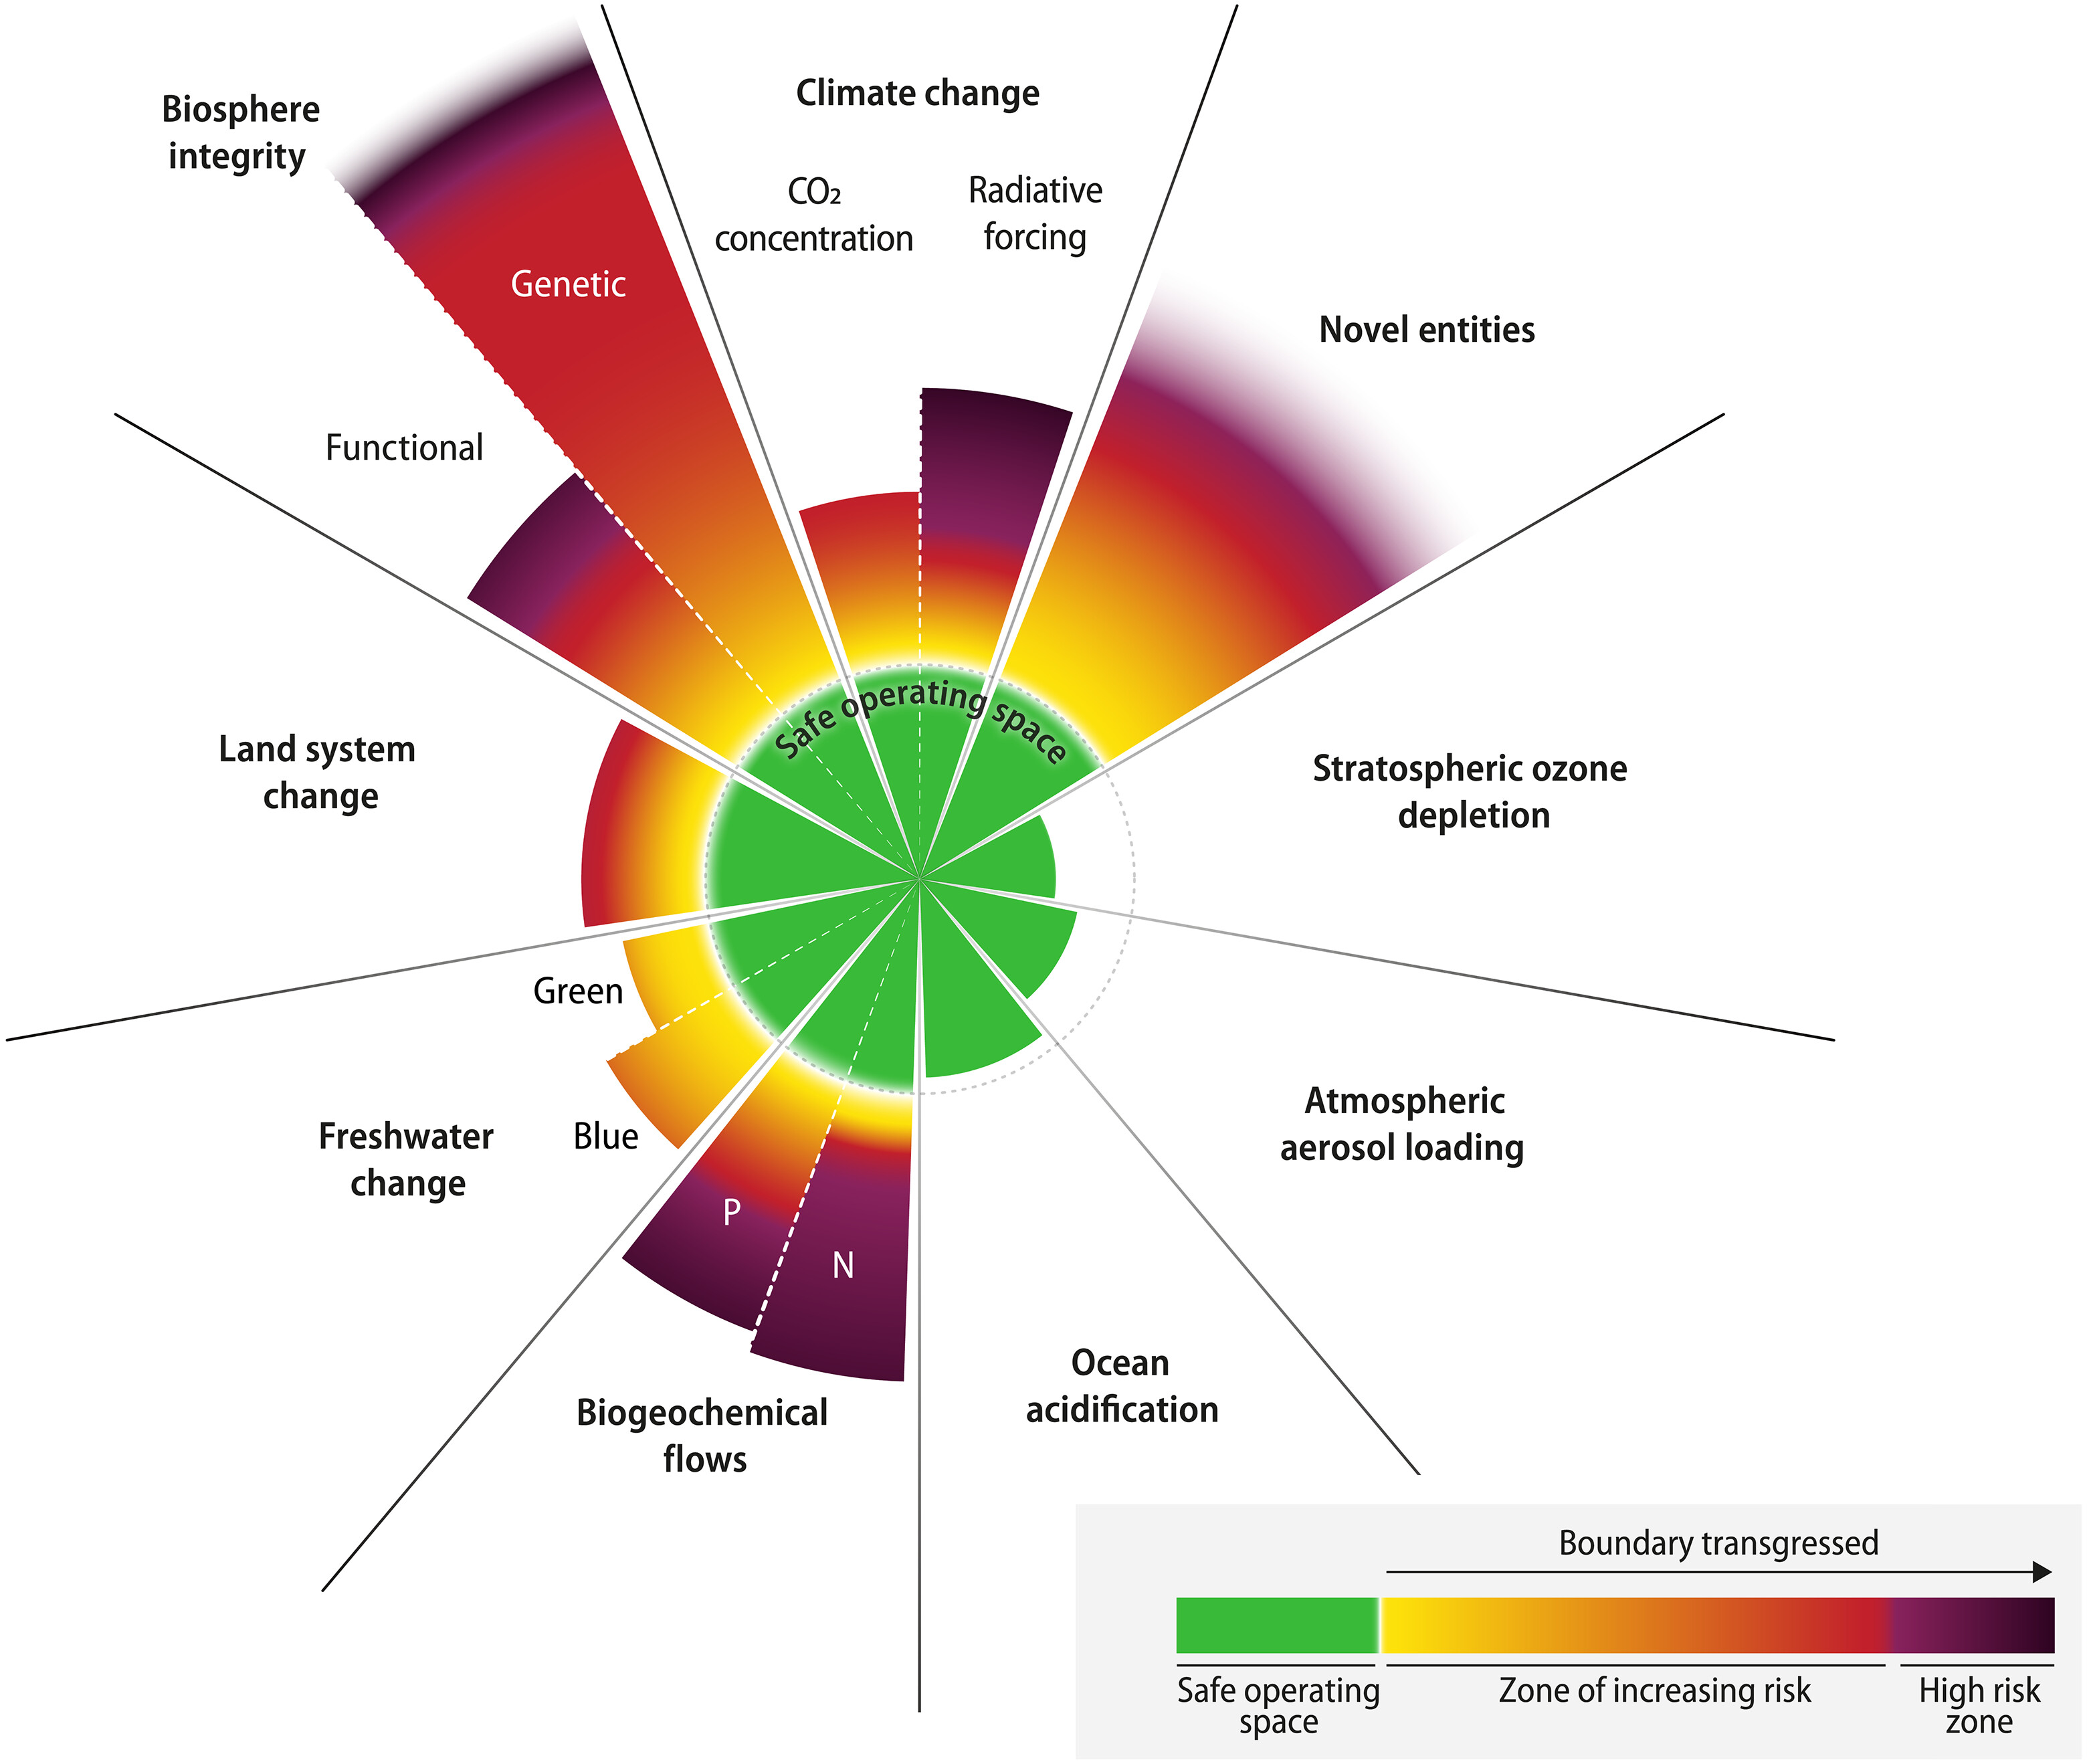
\includegraphics[width= .7\textwidth]{figures/intro/planetary_bounds.jpg}
	\caption{Current status of control variables for all nine planetary boundaries, from \cite{richardson_earth_2023}}
\end{figure}

Among these planetary limits, the integrity of the biosphere has gradually become of particular interest, along with its interaction with other limits, such as climate change, or novel entities (e.g. synthetic organic pollutants, radioactive materials, microplastic pollution...). Created in 2012, the Interdisciplinary Panel on Biodiversity and Ecosystem Services (IPBES) has been raising the alarm on the state of "Nature" globally. Its chair, Sir Robert Watson, put it clearly\footnote{See the \href{https://www.ipbes.net/news/Media-Release-Global-Assessment}{press release address of the 2019 report}}:
\begin{displayquote}
\textit{The overwhelming evidence of the \cite{ipbes_2022_6417333} Global Assessment from a wide range of different fields of knowledge, presents an ominous picture [...]. The health of ecosystems on which we and other species depend is deterioriating more rapidly than ever. We are eroding the foundations of our economies, livelihoods, food security, health and quality of life worldwide}
\end{displayquote}

"Nature" is a central concept in the IPBES framework \citep{ipbes_2022_6417333}:

\begin{displayquote}
\textit{Nature (also defined as living nature) [is] the nonhuman world, including coproduced features, with particular emphasis on living organisms, their diversity, their interactions among themselves, and with their abiotic environment. Within the framing of natural sciences, nature includes e.g. all dimensions of biodiversity, species, genotypes, populations, ecosystems, the biosphere, ecosystem functioning, communities, biomes, Earth life support's systems and their asosicated ecological, evolutionary, biogeochemical processes and biocultural diversity. Within the framework of economics, it includes categories such as biotic natural resources, natural capital, and natural assets. Within a wider context of social sciences and humanities and interdisciplinary environmental sciences, it is referred to with categories such as natural heritage, living environment, or the nonhuman. Within the context of other knowledge systems, it includes categories such as Mother Earth [...], Pachammama [...]}\\
\hspace*{\fill} \small{\cite{ipbes_2022_6417333}, p.14, see also \cite{DIAZ20151}}
\end{displayquote}

Nature, as defined in this approach, is a very large and complex object.
It is defined across ontological and epistemic differences (living and non-living e.g. matter), different types of interactions, at various scales (genotypes v. ecosystems), at different types of processes (biological v. ecological), and across different fields of inquiry (natural sciences v. social sciences). In this dissertation, I study more specifically "biodiversity", which focuses on the variability among living organisms. While it is itself an ambiguous concept, biodiversity tends to put the focus on living organisms, in relation to their material, biotic and abiotic environment (as opposed to the study of the non-living environment) and on its critical role among other components of the Earth system.

The \cite{ipbes_2022_6417333} report documents the drastic changes the biosphere is going through and considers these changes through an anthropocentric lense, i.e. mediating the aforementioned changes through the multiple and diverse contributions that Nature and biodiversity bring to people. It stresses how their disruption impacts human lives and highlights the role of anthropogenic (i.e. of human origin) drivers of the disruption of nature and biodiversity. 
 
This reports sets different objectives to scientific research. The first objective is to explain the feedback mechanisms : how do human livelihoods impact biodiversity? In response, how does biodiversity impact human livelihoods? This objective involves understanding the causes and measuring the direct and indirect anthropogenic drivers of change in nature and biodiversity on the one hand, and on the other hand understanding the channels and scales through which nature and biodiversity contribute to human livelihoods, as well as measuring these contributions. Hence, studying the demise of nature and the potential to remedy it calls for an integrated perspective, that joins natural sciences to social sciences, through frameworks such as social-ecological systems \citep{Ostrom2009} or environmental and ecological economics \citep{daly_ecological_2007}. 
\\
The second objective is to provide a framework to assess the desirability, the feasibility and means of implementation of collective pathways that would remedy the crisis nature is facing. In a way, it involves designing and implementing policy pathways towards sustainable futures, e.g. finding definite courses or methods of action selected from alternatives, at the individual, collective or governmental levels, to achieve future states of the world which remain in a safe operating space regarding planetary bounds \citep{rockstrom2009safe,steffen_2015_planetary}.

In this dissertation, I take on these two objectives using a framework stemming from economics and ecology. A first version of the research questions this thesis aims at solving is: 
\begin{enumerate}
\setlength{\itemsep}{0pt} % No space between items
\item What are the feedback relationships between biodiversity and antropogenic drivers of its decline? 
\item What underlying mechanisms must policy pathways tackle to remedy this demise?
\item  How can integrated economic and ecological approaches be used and refined to analyze inform and design policies? 
\end{enumerate}

In order to refine these questions, I first define the concept of biodiversity, through its natural and social sciences appraisals, and highlight ongoing trends in its demise.

\clearpage


\phantomsection
\addcontentsline{toc}{section}{Emergence and definition of biodiversity as an ecological concept}
\subsection*{Emergence and definition of biodiversity as an ecological concept}


Biodiversity emerged as a concept in the 1980s, along with the emergence of "conservation biology", a branch of biology concerned with the protection of "biological diversity" \citep{soule_what_1985}, as a response to an acceleration in the loss of species. The moral stance of conservation biologoy is that species should be protected for their own sake \citep{soule_conservation_1986}, they have intrinsic value. 
The concept of biodiversity is therefore embedded in an ethical judgement and a call for action. In the wake of the 1992 Rio United Conference on Environment and Development, the \href{https://www.cbd.int/}{Convention on Biological Diversity} emerged as an international treaty to safeguard biodiversity. In doing so, it provided an internationally agreed upon definition:

\begin{displayquote}
\textit{"Biological diversity" means the variability among living organisms from all sources including, inter alia, terrestrial, marine and other aquatic ecosystems and the ecological complexes of which they are part; this includes diversity within species, between species and of ecosystems.}\\
\hspace*{\fill} \small{\href{https://www.cbd.int/convention/articles/default.shtml?a=cbd-02}{Article 2 of the Convention on Biological Diversity}}
\end{displayquote}

This definition highlights a key differentiating feature from other parts of nature, i.e. the living nature of the objects of study. Compared to abiotic factors, biological diversity is characterized by intrinsic growth, reproduction and metabolism (at the individual and population levels), and evolution (at the genetic, and species level). Additionally, these rates of change through time are commensurable with human experience, and most processes (i.e. reproduction, population collapse or recovery, genetic evolution) can be observed within a human lifetime as opposed to the geological temporal scale. 

As highlighted by \cite{VanDyke2008} and \cite{mouysset_diversity_2023}, the definition of biodiversity is difficult, as it recovers ethical, conceptual and measurement dimensions. Biodiversity can be viewed as "an intrinsic, value-ladden quality of natural systems that should be preserved for its own sake" \citep{VanDyke2008, mouysset_diversity_2023}, but it also refers to measurable features.
% relevant to understanding genetic distribution, population levels, community structure (e.g assembly of interacting species in a given area), environmental processes, and ecosystem functions (i.e. the ecological processes performed by living organisms, such as carbon sequestration, nutrient recycling, water filtration etc). 
This definition implies different scales from a hierarchical perspective, at the genetic level, at the species, the community, and the ecosystem levels (defined as the interaction of communities and their abiotic environment). These levels imply different forms of measurement, including the distribution of genes, species abundance (i.e. the number of individuals in a population, at a given time and location), species richness (i.e. the number of different species, at a given time and location) within communities, among communities, and across larger scales (i.e. alpha, beta and gamma diversities.), as well as variations in the abiotic factors that form ecosystems, such as temperature, humidity, water quality, soil quality etc. 
It also comprises different types of diversity : structural diversity (for example, the layers of canopy in forests, the sex-ratio in animal populations), compositional diversity (the variety and abundance of species within a community), and functional diversity (variety of environmental processes performed by living organisms in a given area i.e. carbon sequestration, nutrient cycling or seed dispersal, see \cite{loreau_biodiversity_2002})

\begin{figure}
	\centering
	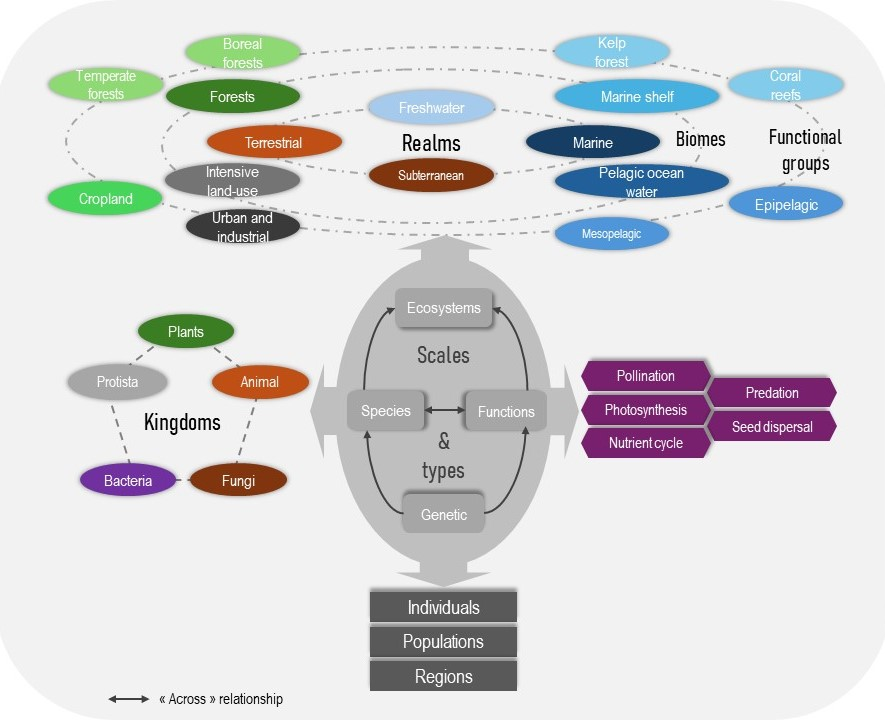
\includegraphics[width =.8\textwidth]{figures/intro/biodiv_illustration.jpg}
	\caption{Biodiversity : a multiform concept across scales and types}
	\label{fig:intro_biod}
\end{figure}

\cite{mouysset_diversity_2023} highlights the difficulty of articulating the definition with common levels in scientific analysis i.e. genetic, taxonomic, and ecosystem, as biodiversity level can fall in between: "populations may be considered from a genetic and taxonomic perspective, or communities that fall between the taxonomic and ecosystem levels". Additionally, as structural and compositional diversity can be seen as the source of functional diversity, the different classes of diversity may be difficult to work with given their colinearity. 

The multiple dimensions of biodiversity highlight several of its critical features. First, it is impossible to measure biodiversity with a single indicator. The study of biodiversity requires multiple indicators to integrally assess the evolution of biodiversity, across scales and types of diversity. The emergence of the concept responds to a desire to protect biodiversity for its own, but also humanity's sake. 

\clearpage

\phantomsection
\addcontentsline{toc}{section}{Nature's Contributions to People: rationales for biodiversity conservation}
\subsection*{Nature's Contributions to People: rationales for biodiversity conservation}


Originally descriptive, ecosystem functions were increasingly viewed from a human perspective starting in the 1970s \citep{hueting1969functions, schumacher1973small}, evolving into the concept of ecosystem services \citep{ehrlich1981extinction} to illustrate biodiversity loss consequences \citep{gomez_history_2010}. This marked a shift from intrinsic to anthropocentric (i.e. given by humans) value \citep{mouysset_diversity_2023}, recognizing biodiversity’s instrumental and relational values—serving human ends and fostering meaningful relationships. Gradually, biodiversity had to be protected for its role in sustaining human life.


%While originally descriptive, ecosystem functions have gradually been referred to from the human point of view (starting in the 1970s, see  \cite{hueting1969functions, schumacher1973small}) and how these functions served human societies, through the concept of \textit{ecosystem services} \citep{ehrlich1981extinction}, as a pedagogical tool to illustrate the consequences of biodiversity loss \citep{gomez_history_2010}.  In this respect, a value switch was operated from an intrinsic value towards an anthropocentric value (i.e. given by humans) standpoint \citep{mouysset_diversity_2023}. In more details, biodiversity features an instrumental value (i.e. serves to achieve a human end) and a relational value (i.e. the importance of desirable, meaningful, and often reciprocal relationships - beyond means to an end) : if biodiversity is to be preserved, it is because of the functions it performs that sustain and improve human life.

The concept gained traction in academic research, and as \cite{Costanza1997} quantified the value of natural capital and ecosystem services, at a staggering 33 trilion \$USD, amounting to approximately 30\% of the 2020 World GDP, the concept reached the policy arena. In 2005, the Millenium Ecosystem Assessment \citep{MEA2005} placed ecosystem services at the center of the policy agenda : it emphasized an anthropocentric value of ecosystem services, but established a dependence of human societies on ecosystem services, and further, on the functioning of ecosystem. In this respect, the Millenium Ecosystem Assessment \cite{MEA2005} was a landmark in safeguarding biodiversity through a \textit{strong sustainability} paradigm (see box 1), and triggered the operationalization of the concept into policy at a large scale (which I will develop later on). The ecosystem services framework was divided into 4 categories, relating to the specific type of services contributing to "human wellbeing" : supporting services (i.e. services allowing for other ecosystem services to be present, including nutrient cycling and primary production) and regulating services ("benefits obtained from the regulation of ecosystem processes" e.g pollination, waste decomposition etc); cultural services ("the nonmaterial benefits people obtain from ecosystems through spiritual enrichment, cognitive development") and provisioning services ("all the products obtained from ecosystems",\cite{MEA2005}, p.54)

\begin{figure}[h]
	\centering
	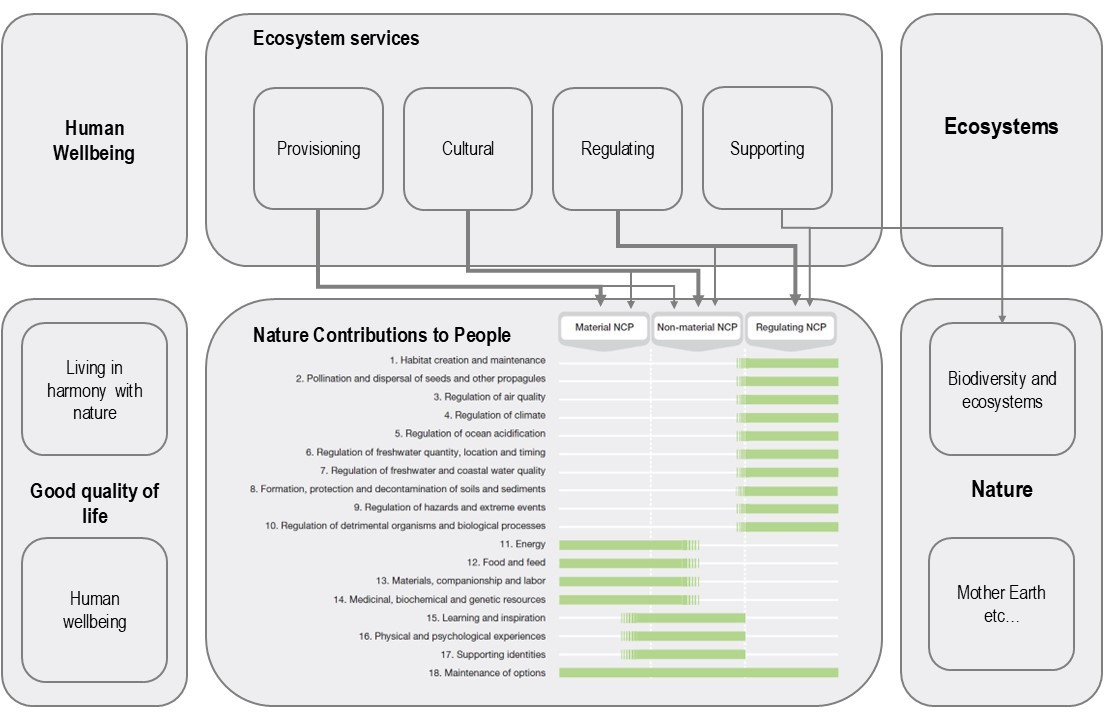
\includegraphics[width = \textwidth]{figures/intro/NCPs2.jpg}
	\caption{Description of the 18 Nature Contribution to People and the connection between the NCP framework \citep{ipbes_2022_6417333} and the Ecosystem Services Framework \citep{millennium2005ecosystems}}
	\subcaption*{Adapted from \cite{diaz_2018} and \cite{ipbes_2022_6417333}}
\end{figure}

Recently, the IPBES platform moved onto a new conceptual framework highlighting Nature Contributions to People (NCP) \citep{DIAZ20151}, defined as "all the contributions, positive and negative, of living nature [...] to people's quality of life \citep{diaz_2018}". This framework underpins 3 types of contributions to people: material contributions to people (flows from nature to people typically consumed to "operate a society or enterprise" (IPBES, p.16), non material contributions (eg. nature's effects on "subjective and psychological aspects underpinning peoples quality of life) and regulating contributions (i.e. "functional and structural aspects of organisms and ecosystems that modify the environmental conditions experienced by people and/or regulate the generation of material and non material contributions"). This framework highlights how Nature Contributions to People can be positive or negative, and depend on the spatial and temporal definition of the contribution, as a given entity can be at the same time the source of positive and negative contributions: for example, forests foster habitat, but also risk endangering people in the event of wildfires. Additionally, it provides a more encompassing view than ecosystem services, as it encompasses perspectives ranging from biodiversity as natural capital employed in an ecological production function (see \cite{polasky_integrating_2009} for a review), as well as perspectives where biodiversity has agency and is linked by reciprocal care obligations to humans \citep{descola}. 

A multifaceted correspondence between the different components and dimensions of biodiversity and its contributions to people underpin human livelihood. The global decline of biodiversity threatens NCPs.

\clearpage
\begin{tcolorbox}[breakable, 
colback=verylightgray, 
colframe=gray!75!black, 
title= {Box 1 - Weak v. Strong Sustainability},
%code={\singlespacing},
fontupper=\small]
\par % This \par ensures spacing before the text starts
\justifying % Start justified text

In 1987, the release of the Brundtland Report \citep{brundtland} provided a broad definition of sustainable development: 

\begin{displayquote}
\textit{In essence, sustainable development is a process of change in which the exploitation of
resources, the direction of investments, the orientation of technological development; and institutional change are all in harmony and enhance both current and future potential to meet human needs and aspirations}\\
\hspace*{\fill}\small{\cite{brundtland}, p.43}
\end{displayquote}

Implementing sustainable development remained an open question. In economics, a "weak sustainability perspective", pioneered by works of \cite{hartwick_intergenerational_1977} and \cite{solow_intergenerational_1986} on exhaustible resources, suggested that "maintaining a non-declining capital stock, which allegedly could be put into practice by investing in manufactured capital all the rents derived from the exploitation of non-renewable natural resources" \citep{gomez_history_2010} was sufficient to maintain consumtpion through time. In this approach, natural capital could be integrally substituted by human made capital. On the other hand, the "strong sustainability" approach advocates advocates for a complementarity, rather than substitutability, of natural resources \citep{costanza_daly}, acknowledging the dependence of humans on ecosystems.
\end{tcolorbox}

\phantomsection
\addcontentsline{toc}{section}{Decline in biodiversity : trends and drivers}
\subsection*{Decline in biodiversity : trends and drivers}

Biodiversity metrics are declinning across all the scales of analysis. The structural conditions of ecosystems, the compositions of ecological communities and populations of species have experienced dramatic changes.\\
The share of unchanged, protected wildlife habitat has plumetted on both land and sea \citep{watson_2016_catastrophic, jones_2018_location} to 23\% and 12\% of space, respectively. At the community level, the share of originally present biodiversity falls bellow 90\% across all biomes, \citep{Hill311787} and local communities are becoming more and more similar \citep{mckinney_1999_biotic}, driven by the increased extent of animal and plant non-alien invasive species, rising by 13\% per decade \citep{seebens_no_2017}. At the species level, to date, global species richness is threatened by a mass extinction, as the global rate of species extinction is at least ten times higher than the average rate over the past 10 million years and is accelerating \citep{barnosky_has_2011, ceballos_accelerated_2015}. On average, 25\% of species are currently threatened with global extinction across a wide range of plant and animal species, on land and at sea \citep{IUCN_redlist_2024}. Using habitat based methods\footnote{ The IUCN Redlist uses detailed accounts for species, in a bottom-up approach, to analyze the extinction risk of species. A top-down approach, relying on the evolution of available habitat and the species-area relationship, uses changes in land use to forecast the extinction of species in a more aggregate manner \citep{Diamond1972BiogeographicKE}}, \cite{Hoskins309377} find that hundreds of thousands of plant and animal species are threatened, and will repay the \textit{extinction debt} caused by anthropogenic changes to their habitats : only 92.1\% of terrestrial vertebrate species, 91.6\% of terrestiral invertebrates and 90.7\% of terrestrial plants have enough habitat to persist. These results suggest that around half a million terrestrial animal and plant species - including over 3000 vertebrates and over 40,000 plants - \textit{dead species walking}, doomed to become extinct, unless their habitats improve in time to prevent it \citep{ipbes_2022_6417333}.

%\begin{figure}[h]
%    \centering
%    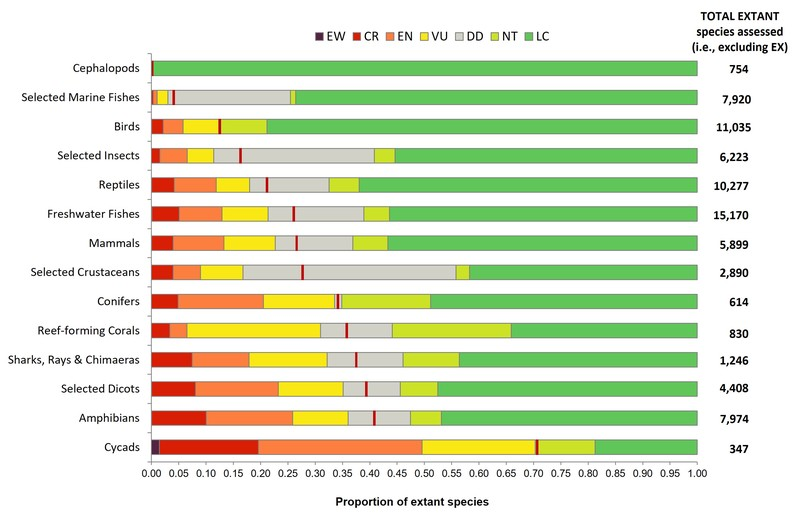
\includegraphics[width=0.8\linewidth]{figures/intro/IUCN_redlist}
%    \caption{The proportion of extant (i.e., excluding Extinct) species in \citet{IUCN_redlist_2024}}
%    \subcaption*{Assessed in each category for the more comprehensively assessed (i.e., at least 80\% of the group has been assessed) groups containing $\geq$ 150 species. Species are grouped into classes. The numbers to the right of each bar represent the total number of extant species assessed for each group. \textbf{EW} - Extinct in the Wild, \textbf{CR} - Critically Endangered,\textbf{ EN} - Endangered, \textbf{VU} - Vulnerable, \textbf{NT} - Near Threatened, \textbf{DD} - Data Deficient, \textbf{LC} - Least Concern.}
%    \label{fig:intro_iucn}
%\end{figure}

Drivers of biodiversity decline are of anthropogenic origin. They can be classified between \textit{direct} drivers, i.e. that directly flow form human actions, such as land use change, anthropogenic climate change, overexploitation, and \textit{indirect} drivers, that can be viewed as the root cause for direct drivers, such as  , changes in the value systems that underpin nature uses (\cite{ipbes_2022_6417333} p.55), demography (urbanization and migration), technology, economy (sectoral transitions, trade expansion) and governance (including risht systems for access to resources).

%The Essential Biodiversity Variables framework \citep{pereira_essential_2013} aggregates fine gridded spatial data into 
A synthesis of natural sciences performed by \cite{ipbes_2022_6417333} outlines the roles of principal drivers at the global scale and across realms (see figure \ref{fig:intro_impacts}).
It shows that land and sea use, reefering to the loss, fragmentation\footnote{Undoubtedly, habitat loss is the main driver of terrestrial biodiversity decline. The effects of fragmentation on biodiversity are highly debated. From a theoretical perspective, models have been developed to study the evolution of populations and communities through space and time, i.e. metapopulation and metacommunity models. Theoretical insights highlight that habitat fragmentation increase the extinction risk, and lower colonization probability, resulting in lower survival and diversity \citep{adler_persistence_1994,hill_habitat_1999, thompson_loss_2017}. At the community scale, increases in diversity among communities (i.e. beta diversity) can emerge from different species resource requirements and the larger spatial extent, hence encompassing more environmental heterogeneity, that results from fragmentation \citep{lasky_reserve_2013, chisholm_species_2018}. However, these effects dampen as habitat loss decreases.  
At the empirical level, the effect of fragmentation is highly debated. According to \cite{fahrig_ecological_2017}, there is no empirical evidence that a group of small habitat patches generally has lower ecological value than large patches of the same total area. Evidence is however found to show that fragmentation does not reduce habitat connectivity, as functional connectivity is improved (i.e. species are in contact with more different resource patches, thus improving the overall functionning of ecosystems). The debate between \cite{fletcher_is_2018} and \cite{fahrig_habitat_2019} surrounds critics based on the ability of statistical models to encompass the effect of fragmentation when habitat loss is present \citep{ruffell_accounting_2016}. Moreover, it reflects the difficulty of landscape ecology, as different mechanisms across scales i.e. patch, landscape and study region, and measures, such as patch size, patch isolation (i.e. distance across patches) and distance to patch edge (i.e. distance to edge within the patch) interact with possible non-linear interactions.}
%
and degradation of wildlife habitat are responsible for 30\% of the impacts on biodiversity. The direct exploitation of wildlife, wild plants and trees represents 23\% of impacts. Climate change, through shifts in biogeographic conditions and changes in habitat, impacts on species traits and genetic evolution represents 14\%, and pollution represents 14\% of impacts. Finally invasive alien species represent 11\%. These drivers have differenciated impacts across ecosystems and biomes \citep{ipbes_2022_6417333}. 

\begin{figure}[h]
	\centering
	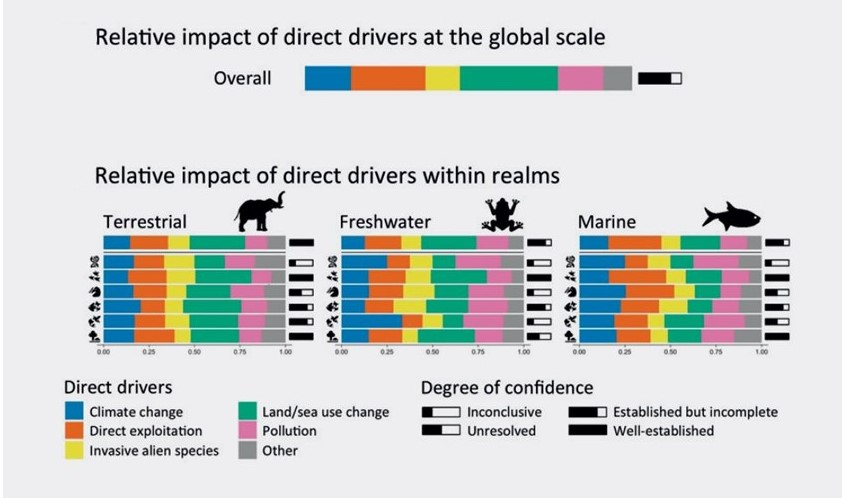
\includegraphics[width = .95 \textwidth]{figures/intro/intro_impactsfin.jpg}
	\caption{Aggregate and realms specific impacts of anthropogenic direct drivers of biodiversity decline adapted from \cite{ipbes_2022_6417333}}
	\label{fig:intro_impacts}
\end{figure}

On land, land use change is the most important driver (30.5\%), driven by deforestation and agriculture, and direct exploitation follows next (21\%). Tropical and subtropical dry and humid forest host the greatest biological diversity. For example, they host the 10 hotspots with the greatest total number of vertebrates \citep{mittermeier_global_2011}. In such forests, habitat loss and degradation are the main drivers of reductions in species abundance and richness \citep{newbold_global_2014}. Legal and illegal selective logging destroy habitat \citep{hoare2022establishing,  bousfield_2023_large} and are combined with hunting and poaching of wildlife \citep{gallego_2020_combined}, generating between 60 and 180 billions  \$ USD of revenue \citep{gfi_2017}\footnote{Illegal wildlife trade represents between 5 and 23 billion \$USD, while illegal logging represents 52 to 157 billion \$USD}. 

For marine species, overexploitation is the main driver (29\%) \citep{ipbes_2022_6417333}. With 90 million tons of capture  (and 141 billion \$ USD)  in 2020 \citep{fao_2022_state}, fisheries stock within biologically sustainable levels have decreased to 64.6\% in 2019, from 90\% in 1974\footnote{ In this calculation, all fishery stocks are equally counted, irrespective of their abundance or catch}, driven by overfishing in the Southeast Pacific and the Mediterranean and Black seas. Nonetheless, illegal, unreported and unregulated (IUU) fishing is a threat to fisheries. Estimates from 15 years ago \citep{agnew_estimating_2009} estimated it represented between 11 and 26 million tonnes of fis with a value of 10 to 23 billion \$ USD. 
 
Additionally, anthropogenic climate change drives ecosystem disruptions on land \citep{burrell_anthropogenic_2020, conradi_reassessment_2024} and at sea \citep{gomes_marine_2024}, through changes in various channels including ecological suitability and foodweb disturbances. On land, for example, mediterranean forests, woodlands and scrubs, covering 4 million km$^2$, are areas of exceptionally high diversity too \citep{Mooney2001, blondel_2010}, threatened with urban expansion and increased wildfire risk. Wildfire frequency and severity are expected to increase with global warming \citep{Dupuy2019ClimateCI}, causing important direct and indirect costs to society including destruction of infrastructure and perturbations to economic activity \citep{wang_economic_2021}, smoke related health conditions \citep{burke_wildfire_2023, heft-neal_behavior_2023}, disrupting structural features of ecosystems \citep{Ayars2023} and threatening biological diversity \citep{Wintle2020}.

\phantomsection
\addcontentsline{toc}{section}{Economic challenges of anthropogenic drivers of biodiversity decline}
\subsection*{Economic challenges of anthropogenic drivers of biodiversity decline}

Habitat loss and overexploitation present both common and differentiated challenges. A common identifiable cause is the large opportunity cost of preserving a species habitat, or existence, in the presence of other economic alternatives for land and time, as well as financial constraints. Additionally, habitat loss and overexploitation share a temporal dynamic aspect, where immediate actions have durable consequences, possibly irreversible.

Habitat loss and fragmentation in terrestrial ecosystems present specific challenges. Forests, for example, serve multiple uses (or NCPs) to various agents: loggers profit from timber, settlers clear land for agriculture, hikers seek pristine landscapes, and conservationists aim to restore natural cycles. Forests also hold spiritual and cultural value, creating conflicts among these uses. For instance, deforestation and urbanization destroys both habitat and sacred land, but create measured economic value \citep{giglio_economics_2024} while wildfire prevention can damage wildlife habitat \citep{bradshaw2018}. Species can also have mixed impacts; deer, for example, are valued at low densities but cause damage at higher densities \citep{putman_identifying_2011}. 
%Climate change worsens habitat loss by altering habitat distribution and increasing threats like wildfires \citep{Dupuy2019ClimateCI,wasserman_climate_2023}\\
A second key feature to halt habitat fragmentation is considering the integral set of interdependencies, ecological spillovers and economic externalities that underlie the spatial dimension. The configuration of space, and species movement is at least partly the result of an economic decision. Maintaining habitat connectivity involves identifying patches and paths to be conserved or restored that contribute most to it, in the form of corridors, ecoducts or stepping stones \citep{Turner2005, Turner2011}. The value of patches and paths for connectivity is intrinsically linked to their surrounding : at the same geographic location, a patch has differential value for biodiversity habitat if it is connected to others, or if it is isolated (see box 2). When paths are beyond human control, patches have different importance based on their location, and when the location of patches is fixed, the extent of paths and their location is paramount. Third, as multiple actions and uses structure connected elements of ecosystems (i.e. different tracts of land, or different biodiversity scales), they trigger spatial spillovers i.e. consequences that go beyond their \textit{in situ} effects. When these spillovers are not taken into account by the agents that generate them, they can be called "dynamic spatial externalities" \citep{sanchirico_bioeconomics_1999, costello_optimal_2008, costello_private_2017}. As halting habitat loss and fragmentation involves conserving tracts of land, neighboring parties may very well benefit (or suffer) from more wildlife and ecosystem (dis-)services on their property, through time. As agents respond to each other's action profiles, they behave strategically, both in space and time. These externalities can trigger specific problems of "race to the bottom" \citep{costello_private_2017} : when neighboring parties of a decision maker that undertakes conservation, or risk reduction, fail fail to reciprocate as they benefit from spillovers, a vicious circle of least action is triggered. Conversely, when ecological spillovers are positive, this may lead everybody to use a resource at unsustainable levels, even in the presence of well defined rights, absent other mechanisms \citep{janmaat_sharing_2005,kaffine_unitization_2010}. 
 Hence, habitat fragmentation and overexploitation are interrelated through spatial connectivity. Fourth, improving habitat loss and fragmentation involves coordinating numerous actors towards increasing the area and connectivity of habitat, while taking into account the associated costs and benefits, and different interests.
 In some cases, the financial constraints, the magnitude of costs associated with increased habitat connectivity and the difficulty of coordination warrant a public policy where a central planner undertakes the action \citep{Mouysset2012}. On the other hand, mechanisms to decentralize efficient spatial planning exist and can be efficient under limited costs of cooperation \citep{costello_private_2017, bareille_agglomeration_2023}. 
 
	Halting overexploitation requires understanding and addressing its motives. Overexploitation (or under control, for pests), results from an imbalance between the appropriation and incumbance of Nature's contributions to people (both positive and negative) and the socially desirable level and allocation of these contributions, as well as the uncoordinated, strategic behavior of agents. 	
	The common nature of most natural resources \citep{Gordon1954, smith_models_1969} has long been identified as one of key reason for their demise: numerous events have shown a "race to the bottom", where the absence of secure property rights hastened the overharvest and decline of populations. It has long been the center of attention, and mechanisms relying on property rights assignment have been studied extensively \citep{libecap_tragedy_2009, costello_partial_2015, isaksen_tragedy_2019}.
	
\begin{tcolorbox}[breakable, 
colback =verylightgray, 
colframe=gray!75!black,
title={Box 2 - Habitat Loss, Fragmentation and Connectivity},
%code={\singlespacing},
fontupper=\small]


\par % This \par ensures spacing before the text starts
\justifying % Start justified text

Habitat loss refers to the loss of areas featuring suitable environmental conditions for species survival and development. At a constant habitat area, fragmentation refers to increases in the number of patches and decrease in the mean size area of each patches, as in figure \ref{fig:connectivity_intro}. \\
Landscape connectivity is defined in relation to fragmentation. It measures "the degree to which the landscape facilitates or impedes movement among resource patches" \citep{taylor_connectivity_1993}. 
It recovers a \textit{structural} dimension, which describes the physical arrangements across patch and a \textit{functional} dimension, which emphasizes the ability and realization of movements of individuals through the landscape.

 Aggregate connectivity measures take into account the role of differentiated patches and paths. In panel D of figure \ref{fig:connectivity_intro}, the circled patches play an instrumental role in maintaining connectivity. Habitat patch 1 and 2 have the same number of connected patches. However, patch 1 is maintains the connection between the east and west habitat patches in the landscape, and is connected to highly connected patches. Removing habitat patches 1 and 2 would have larger consequences on habitat than removing other identical size patches. Similarly, removing the dotted path (bottom left of panel D) would isolate patch 3, while removing the dashed path would not leave patch 4 isolated. Hence, paths and patches have different impacts on connectivity, depending on the surrounding patches and paths.
\\% Adds some space before the image
\begin{center}
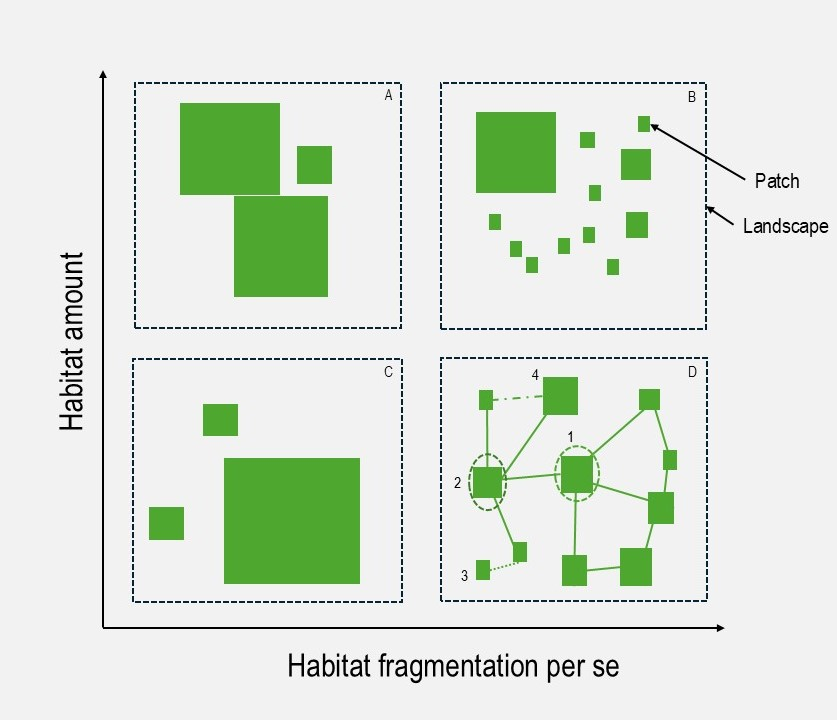
\includegraphics[width = .8\textwidth]{figures/intro/fragmentation.jpg}
\captionof{figure}{Illustration of the effects of habitat loss and fragmentation, adapted from \cite{fahrig_habitat_2019}, and of connectivity}
\label{fig:connectivity_intro}
\end{center}
\end{tcolorbox}
\clearpage
	
	 However, while property rights may be assigned, they can be notoriously hard to enforce in areas where regal functions are challenged: \textit{de facto} rights are assigned and enforced. In this case, the common nature of the resource may not be the main concern: local market concentration forces may outweigh overexploitation forces, even in the presence of some of form of open access \citep{damania_economics_2007}. 
Around the world, wildlife poaching and trade typically originates from organised crime groups, and is associated with different criminal activities \citep{mozer_introduction_2023}.  Concentrated markets tend to emerge and characterize wildlife markets, as competition is hindered by violent organised crime groups. In this case, resource management is strategic and responds to market characteristics (demand structure, intermediary input price) and ecological characteristics (distribution of species, biological growth rate, carrying capacity\footnote{The notion of \textit{carrying capacity} has been used since the mid-XXth century by population ecologists (for a history of the notion, see \cite{sayre_carrying_2008}) to describe the maximum population size of a species a given ecosystem can sustain in the long run.} of the ecosystem)\\
	At one extreme, locally monopolistic markets structure for wildlife products may emerge, especially in the case of endemic species (i.e. native and restricted to an area).
They may be the conservationists' bestfriend \citep{solow_resources_1974, hannesson_note_1983}, depending on specific, context dependent market and species characteristics, as a monopolist has an interest in restricting supply to increase prices, if consumers do not react too much (i.e. under limited demand elasticity). A vast range of  market structures \citep{damania_economics_2007, hannesson_effects_1985} sticking to real world situations have been studied. However, the full range of interactions between a species endemism, local market power, cost of effort and access to final consumer markets require more analysis to clarify the impact of market structure.\\
	Other drivers of overexploitation can be found in the large expected benefits (relative to other local economic activity) some natural resources can bear, most of the time because of their rarity (i.e. absence of economically viable substitute), whether today or in the future \citep{Kremer2000}. While the effects of substituting man-made products to disrupted ecosystem services are starting to get empirically studied \citep{frank_economic_2024} and show how dreadful costs can be, the effect of introducing substitutes to illegally poached wildlife products can be an example of strong substitutability between natural and man-made assets \citep{chen_economics_2017}. As broader forces affect overexploitation, including poverty, it is clear that adressing overexploitation implies generalizing conclusion from the interplay of a single species with the institutional setting, how a  species' future interacts with the availability of substitutes, and how the distribution of revenues from sustainable harvests may foster a reasoned use of the resource. 
	
	A wide range of policies have been implemented at different organisational levels, to jointly or separately halt the identifed drivers of biodiversity decline on land and at sea, with varying degrees of success. 

\phantomsection
\addcontentsline{toc}{section}{Biodiversity policies : from global to local}
\subsection*{Biodiversity policies : from global to local}
\par
Successive international policy frameworks have sought to halt biodiversity loss by addressing its drivers comprehensively. In 2022, the 15th conference of the UN Convention on Biological Diversity launched the \href{https://www.cbd.int/doc/c/e6d3/cd1d/daf663719a03902a9b116c34/cop-15-l-25-en.pdf}{Keunming Montreal Global Biodiversity Framework (GBF)}, replacing the Strategic Plan for Biodiversity 2011-2020 and the Aichi Targets after the failure to meet its objectives\footnote{Among the 20 Aichi Targets, none were globally met in 2020, and only 6 were partially met including the identification and eradication of invasive species on islands, the setting of 17\% of terrestrial and inland water areas and 10\% of coastal and marine areas as conservation areas, the implementation of policy instruments and effective national biodiversity strategy and planning, and the increase in financing biodiversity protection. Reasons invoked for the failure were the lack of clear indicators to assess targets, and no obligation to report on progress towards achieving the targets  \citep{maron_setting_2021}}. The GBF sets four global goals for 2050, with 23 measurable targets to halt biodiversity loss by 2030. These goals include maintaining ecosystem integrity and connectivity and preventing human-induced extinctions (Goal A), sustainably using biodiversity (Goal B), sharing conservation benefits and burdens equitably (Goals C and D)\footnote{See \href{https://www.cbd.int/doc/c/e6d3/cd1d/daf663719a03902a9b116c34/cop-15-l-25-en.pdf}{Section G. Kunming-Montreal Global Goals for 2050}}. \href{https://www.cbd.int/gbf/targets/5}{Targets} include restoring 30\% of degraded ecosystems, conserving 30\% of land and sea areas, and ensuring the sustainable use and management of wild species.



%\begin{tcolorbox}[breakable, 
%colback=verylightgray, 
%colframe=gray!75!black,
%title={Box 3 - The Convention on Biological Diversity and the Aichi Targets},
%code={\singlespacing},
%fontupper=\small]
%\label{box:policy_frameworks_for_biodiv}
%\par % This \par ensures spacing before the text starts
%\justifying % Start justified text

%In 2010, the Convention on Biological Diversity set its "Strategic Plan for Biodiversity 2011-2020", structured around the 20 Aichi Biodiversity Targets, spanning over 5 goals :

%\begin{itemize}
%\item Goal A : Address the underlying causes of biodiversity loss by mainstreaming biodiversity across government and society
%\item Goal B : Reduce the direct pressures on biodiversity and promote sustainable use
%\item Goal C : To improve the status of biodiversity by safeguarding ecosystems, species and genetic diversity
%\item Goal D : Enhance the benefits to all from biodiversity and ecosystem services
%\item Goal E : Enhance implementation through participatory planning, knowledge management and capacity building
%\end{itemize}

%In 2020, the Global Biodiversity Outlook 5 \citep{global_biodiversity_outlook} showed that none of the Aichi %Target were globally met, and only 6 targets were partially achieved, including the identification and eradication of invasive species on islands, the setting of 17\% of terrestrial and inland water areas and 10\% of coastal and marine areas as conservation areas, the implementation of policy instruments and effective national biodiversity strategy and planning, and the increase in financing biodiversity protection. 

%While several elements showed progress, the failure of the 2011-2020 Strategic Plan was patent. Measurable indicators to assess progress towards targets were missing. This was tackled with the new Global Biodiversity Framework that took over in 2020, although with severe limitations. According to critics \citep{maron_setting_2021}, the current framework also lacks ecological scale-specific indicators (for genes, species, ecosystems) and do not provide specific net outcome statements (such as the 1.5C degree target of the Paris Agreements) across areas, nor a clear implementation timeline. 

%Additionally, the 2011-2020 Strategic Plan failed as countries did not have to report on their progress, only declare their targets. The 2020 Global Biodiversity Framework has implemented follow-up measures : although it is not a legally binding frameworks, countries who have signed commit to demonstrating progress towards the targets and update their National Biodiversity Strategy and Action Plans (see section B.5 and section J of the \href{https://www.cbd.int/doc/decisions/cop-15/cop-15-dec-04-en.pdf}{GBF})
%\end{tcolorbox}
Other international treaties, such as the \href{https://cites.org/fra}{Convention on International Trade in Endangered Species (CITES)} established in 1973, regulate trade in endangered species to prevent illegal wildlife trade\footnote{CITES features 183 member parties (countries), it lists species across "appendices", with varying degree of protection of the species and restrictions limiting the trade in endangered species.\\
Appendix 1 : the most endangered species, threatened with extinction and prohibited international trade, except when the purpose of exports is not commercial\\
Appendix 2 : species that are not necessarily now threatened with extinction but that may become so unless trade is closely controlled\\
Apppendix 3 : species included at the request of a Party that already regulates trade in the species and that needs the cooperation of other countries to prevent unsustainable or illegal exploitation} and promote species survival. Despite its scope, CITES’ effectiveness is debated. Local enforcement \citep{HEID2023102784} and demand reduction campaigns \citep{macfarlane_reducing_2022, moorhouse_demand_2024} are critical, but trade bans can sometimes increase prices and poaching incentives \citep{hsiang_does_2016}. In some cases, conservation farming has succeeded by “flooding the market” \citep{gentry_looking_2019, phelps_framework_2014, tensen_under_2016}. Supply-side interventions have occasionally succeeded at reducing poaching and recovering wild populations – i.e. vicuña and spotted cat \citep{iucn_world_2000, sahley_biological_2007} – but they have also failed – i.e. green python, African elephant \citep{lyons_wildlife_2011, hsiang_does_2016}. Uncertainty around conservation outcomes from market-based approaches has led to continued reliance on trade bans and controls that are often ineffective at reducing poaching.

National and supranational policies have also been key. In the U.S., policies like  \href{https://www.fs.usda.gov/Internet/FSE_DOCUMENTS/fseprd645666.pdf}{Wilderness Act of 1964} created protected areas to preserve habitats. In the wake of the environmentalist movement of the 1960s and 1970s, landmark regulations aimed at protecting natural habitats, such as the \href{https://www.epa.gov/laws-regulations/summary-clean-water-act}{Clean Water Act of 1972} (ensuring sewage to limit the disruption of wildlife habitat), and specifically targeted towards species conservation with the \href{https://www.fws.gov/sites/default/files/documents/endangered-species-act-accessible.pdf}{Endangered Species Act of 1973}. Results of the Endangered Species Act are debated. While the impacts seem to be overall positive on species recovery, budget dedicated to listings are slim, and the associated costs are substantial and concentrated on private landowners while benefits are more broadly distributed \citep{brown_economics_1998, langpap_economics_2018}.
%
Localized initiatives, such as the \href{https://y2y.net/}{Yellowstone Yukon Conservation Initiative} (1993), connect ecological areas across the U.S. and Canada, using private conservation schemes and local policy making. 
%
In Europe, the Natura 2000 network\footnote{A system of protected areas, established in application of the European Union Birds Directive (1976) and Habitats Directive (1992), and formally in place starting the mid 2000s} has created the largest conservation area globally, covering 18\% of land and 9\% of marine regions in the EU, across 28,000 sites. In broad strokes, it delineates conservation areas of ecological interest where development and human activities are restricted. Its ambition stemmed from taking into account the scale of biodiversity processes rather than administrative boundaries to develop an interconnected network of conservation areas. The ecological and economic performances of such a network are substantial, as they generate spatial spillovers both in terms of economic and ecological performance \citep{cocco_relaxing_2023}.

Acknowledging that biodiversity habitat can be seen as a continuum between unsuitable and suitable conditions, mechanisms such as Payments for Ecosystem Services (PES) are leveraged to incentivize conservation on agricultural land. Taking into account the ecological spillovers of decreased spillovers, payments for ecosystem services with agglomeration bonuses, such that neighbors gain an additional marginal benefit when a new local participant implements conservation measures, can be efficient \citep{parkhurst2002agglomeration, bareille_agglomeration_2023}. Overall, the spatial consequences of decentralized policies has yet to be fully integrated in policy making.

Finally, some policies aim at mitigating the threats posed by climate change on ecosystems and species, by changing landscape connectivity. In mediterranean forests, where biodiversity is exceptionally high but wildfires are an ever growing threat \citep{Dupuy2019ClimateCI, wasserman_climate_2023}, fuel treatment operations\footnote{Mechanical thinning, prescribed burns, and sometimes, logging, have been leveraged to decrease the fuel load in risky areas and theoretically decrease the probability and severity of burns upon wildfire occurence. In numerous regions, such as conifer forests in California \citep{Vaillant2009, Kalies2016, low_shaded_2023}, eucalypt forests in South Western Australia \citep{burrows2013, boer_long-term_2009, Florec2020}, southern Europe \citep{Fernandes2013}, evidence shows that fuel treatments, can mitigate wildfire intensity and spread. Land management agencies have historically implemented these policies in Australia \citep{burrows2013}, Europe, and the United States (and are projected to ramp up, for example under the Infrastructure Investment and Jobs Act of 2021 in the US)} limit the occurence and severity of wildfires. Public policy is leveraged in the face of increasing risk, limited insurability and threats to biodiversity. For example, with limited insurability of homes in the wildland urban interface in California\footnote{For example, \href{https://www.washingtonpost.com/climate-environment/2024/08/29/california-insurance-wildfires-allstate/}{200,000 homeowners will see an increase in their insurance premium} by an average of 34.1\% from Allstate insurance in November 2024. In 2023, the FAIR plan, designed to be the insurer of last resort in California (state mandated but privately funded) saw a \href{https://www.cfpnet.com/key-statistics-data/}{38.3\% increase in its total exposure.}}, as well as the potential economy-wide human and non-human damages from wildfires \citep{wang_economic_2021, heft-neal_behavior_2023, Ayars2023} state-mandated and operated fuel treatment policies are of the essence. However, with increased budgets and improved spatial planning, these policies could achieve better performances in reducing risk while protecting biodiversity.\\
Decentralized policy mechanisms exist, such as mandates to create a defensible buffer around individual properties : in California, a 100-foot defensible around houses is mandated in State Responsibility Areas,and can translate in reduced insurance premia;  in France, in dedicated regions, the "obligation de débroussaillement" mandates fuel control operations in a 50m radius to "decrease the intensity of wildfires and limit their spread"
\footnote{Translated by the author - \href{https://www.legifrance.gouv.fr/codes/article_lc/LEGIARTI000047809197}{Article L131-10} of the Code Forestier} with fines reaching $5,000$ euros for failing to comply.


I focus on the analysis of the interplay between biodiversity and human actions, through the NCPs it provides and the anthropogenic drivers of its decline. As existing policies have had varying degrees of success in halting biodiversity decline, a framework for policy design is required. I use a framework stemming from ecology and economics to jointly analyze the causes of this decline and provide policy recommendations. 

\phantomsection
\addcontentsline{toc}{section}{Biodiversity as an economic object}
\subsection*{Biodiversity as an economic object}

The definition of economics has expanded with new methods and objects but primarily focuses on analyzing human behavior at individual and collective levels to manage scarce resources across alternatives \citep{mankiw_principles_2011, bade_foundations_2002, backhouse_retrospectives_2009}. This leads to two goals: understanding and explaining the state of the world (positive approach) and determining the best ways to manage resources (normative approach). Economics thus provides tools to analyze biodiversity loss and design policy.

However, applying economics to biodiversity is challenging. It requires the commensurability of values, often through monetary valuation. Initially, biodiversity was valued for its products (hunting, fishing, logging) traded at market prices, focusing on resources in a specific state—dead. This approach captured only part of the "use value" of species \citep{Krutilla1967} (in the NCP framework, the material NCPs associated with food and materials), failing to consider their full value. Over time, the notion of "use value" expanded to include species' direct and indirect contributions. Many studies have used market proxies to estimate biodiversity's price\footnote{For instance, hedonic methods \citep{rosen_hedonic_1974} use variations in market prices for goods like real estate linked to environmental features, while the travel cost method \citep{clawson_economics_1967, bhandari_willingness_2010} measures consumer spending on experiences like wildlife viewing.}. Where market proxies fail, for lack of data for example, non-market valuation techniques have emerged \citep{carson_contingent_2012}, relying on stated preferences\footnote{For example, following the Exxon-Valdez spill in 1989, surveys were developed to estimate the value of affected biodiversity by asking people's willingness to pay for recovery \citep{carson_contingent_1992, arrow_report_1993, carson_contingent_2003}, though these methods are controversial \citep{Diamond94}} (i.e. declared rather than observed willingness to pay). 
%However, making the economics of biodiversity is not an easy task. 
%Management requires a commensurability of objects in terms of values (not necessarily with the same indicators, but a basis for rational comparison). Hence, a first step involves finding a common measurement, which has often implied monetary valuation. The valuation of biodiversity started with the valuation of its products :  hunting, fishing, logging have always been instrumental in human livelihoods, its products became economic objects to be traded with an established market price. This approach only considered said resources through a particular ontological state : dead. 
%Focusing on single species, this approach was only able to elicit the part of the "use value" of species (see \cite{Krutilla1967} and in the modern NCP framework, the material NCPs associated with food and materials) and not the integral value of species \citep{Krutilla1967}. The notion of "use value" had to be broadened to encompass the direct and indirect contributions of species, through a variety of techniques, and put a monetary value on them. A wealth of research has relied on market proxies, where market price for goods and services associated with biodiversity feature, were used to derive the price of biodiversity\footnote{On the one hand, hedonic methods \citep{rosen_hedonic_1974} have used the variation in observed market prices for a variety of goods, such as real estate, related to the variation of environmental and biodiversity features, and have studied how these variations have been internalized in goods market prices. On the other hand, methods such as the travel cost method \citep{clawson_economics_1967, bhandari_willingness_2010} have relied on observed consumer behavior and expenditures to experience "Nature", such as wildlife seeing, to elicit the price people are willing to pay for biodiversity}. When impossible to apply, for lack of proxy or data, other methods have relied on non-market valuation techniques \citep{carson_contingent_2012}, eliciting people's willingness to pay using stated preferences\footnote{For example, in 1989, the tanker Exxon-Valdez spilled close to 42 million liters of oil in Alaska, in an ecologically sensitive area : marine populations were decimated. According to \href{https://darrp.noaa.gov/oil-spills/exxon-valdez}{the National Oceanic and Atmospheric Administration}, an estimated 250,000 seabirds were killed, 2,800 sea otters, 22 killer whales, billions of salmons were killed. Numerous species are not in recovery after 25 years. In order to hold Exxon accountable, surveys were developped to assess the value of marine biodiversity, by surveying the willingness of people to pay for wildlife\citep{carson_contingent_1992, arrow_report_1993, carson_contingent_2003}, with controversed success \citep{Diamond94}}. 
With the ecosystem services framework, valuation techniques were scaled to capture various services \citep{Costanza1997}, including recent modeling global modeling efforts \citep{giglio_economics_2024}. Multiple methods extended biodiversity valuation across scales, from genetics to habitats and functions \citep{bartkowski_capturing_2015}.
Recently, approaches shifted from direct monetary metrics to assessing species' effects on outcomes like health \citep{frank_social_nodate,frank_economic_2024}. A significant body of research rejected monetary valuation, focusing instead on biodiversity metrics to weigh against economic outcomes \citep{Mouysset2011, Watzold2016a}. These metrics help assess or plan biodiversity evolution with a scientific measurement, rather than through incomplete monetary valuation. 

%With the rise of the ecosystem services framework, valuation techniques were developed at a broad scale to encompass the various services \citep{Costanza1997}. Overall, a variety of methods has been leveraged to extend the valuation of biodiversity at different scales, ranging from genetics to habitats, and encompassing functions \citep{bartkowski_capturing_2015}.
%In recent years, these approaches have been further developed by departing from direct monetary metrics, towards measuring the influence of species on other outcomes such as health \citep{frank_social_nodate,frank_economic_2024}. 
%A large strand of research refused to include direct monetary valuation, and chose to focus on biodiversity metrics to be weighed against monetary outcomes \citep{Mouysset2011, Watzold2016a}. These metrics can be used to assess the evolution of biodiversity, or to plan it. 

Managing biodiversity involves balancing alternatives while accounting for the specificity of living elements, regeneration and extinction rates, which requires understanding its temporal dynamics. Economics provides a framework to model these dynamics and assess the impact of different actions on current and future biodiversity. Models, as "stories with structure" \citep{GibbardVarian}, where the structure is "the logical and mathematical form of a set of postulates" with "elements of interpretation" \citep{GibbardVarian}, are used for a variety of purposes (see box 3).
Alongside the evolution of monetary valuation techniques, "bioeconomic" models have been developed to design policies for resource management and biodiversity conservation.\\

%Weighing the different alternatives, across uses of biodiversity, across means of preserving it, requires factoring the specificity of biodiversity : regeneration rates are commensurable with human experience, and potentially, extinction rates. From an epistemological standpoint, this implies considering the temporal dimension of the resource. Economics provides an explicit framework to consider the temporal dynamic of biodiversity and the consequences of different actions on its current and future state through the use of models. Models are "stories with a specified structure", where the structure is "the logical and mathematical form of a set of postulates" with "elements of interpretation" \citep{GibbardVarian}. Using mathematics, models can be used for a variety of functions (see box 3). In an other strand of research, alongside the evolution of monetary valuation techniques, \textit{bioeconomic models} have been developed to design policies for resource management and biodiversity conservation.
%\clearpage

\begin{tcolorbox}[breakable, 
colback=verylightgray, 
colframe=gray!75!black, 
title= {Box 3 - What do models do? },
%code={\singlespacing},
fontupper=\small]

\cite{varenne_epistemologie_2014} furthers the approach qualifying models as "mediators" between the real world and scientific thought, and labels models as "facilitators", across multiple dimensions. A non-exhaustive typology of the roles models can play includes (i) a pedagogical role (facilitating communication), (ii) a predictive role (facilitating anticipation), (iii) a heuristic role (facilitating the explanation of a mechanism with a few simple interactions), (iv) prescriptive (facilitating the response to a given problem) and (iv) integrative (facilitating exchanges between disciplines). 

\end{tcolorbox}


\phantomsection
\addcontentsline{toc}{section}{Bioeconomic modeling for the study and management of biodiversity}
\subsection*{Bioeconomic modeling for the study and management of biodiversity}

Bioeconomic models are analytical tools (i.e. with a mathematical  formulation) that jointly model the feedbacks between components of biodiversity in wild or weakly manageed ecosystems and economic activities, at different levels (e.g micro, mezzo and macro levels). They blend together a decision model emerging from economic theory, and the dynamics of biodiversity elements from ecology. Bioeconomic models \citep{Gordon1954, smith_models_1969, clark_profit_1973} have emerged from joint efforts by economists and ecologists to manage resources accounting for the specific dynamics of biotic elements \citep{Parent_Mouysset_Missemer_Levrel_2024}\footnote{As highlighted in \cite{Parent_Mouysset_Missemer_Levrel_2024}, the concavity of the "ecological production function" i.e. of landings, resulted from the application of the law of decreasing returns to human effort. It was only with Schaeffer's input that the concavity of the ecological production function in \cite{Gordon1954} became grounded from an ecological point of view, stemming from a population dynamics argument (using a logistic growth function)} as truly interdisciplinary models (see box 4). 

Historically, the first bioeconomic models have emerged from population ecology and static economic analysis, to study the management of fisheries. The Gordon-Schaeffer \citep{Gordon1954, Schaefer1954} model highlights the evolution of a fish population according to different harvest regimes, and aims at maximizing revenues in equilibrium. It distinguishes effort levels between those providing the maximum economic yield (i.e. resulting in the economic profit) from those providing the maximum sustainable yield (i.e. resulting in the largest fish growth), yielding new policy perspectives: as the maximum sustainable yield effort is larger than the maximal economic yield, the policy target should be the latter. Aiming for the maximum economic effort would therefore yield larger fish populations and promote economic efficiency, compared to unregulated, open-access. The original model was later extended to account for transitory dynamics and integrate elements from capital theory, focusing on the dynamic allocation of resources through time \citep{smith_models_1969, clark_profit_1973}. 

In the 1970s, economic decision making was applied to the progression of pests in forests and agriculture \citep{Hueth1974, Feder1975}, and the bioeconomic modelling framework was soon applied to study the optimal management of species, both goods and bads i.e. large game and forestry v. invasive pests, leveraging single population dynamics, without much spatial processes \citep{swanson_economics_1994, Skonhoft1999_on,ALEXANDER2000, Horan2002}.  In the 1990s, a second strand of bioeconomic models started to focus on the optimal conservation of species at the community level to find the mechanisms to conserve biodiversity through habitat management, ranging from reserve design to agricultural policies to foster conservation \citep{costello_dynamic_2004, Polasky2001,Polasky2005, Watzold2016a, Mouysset2011}. The two strands developed and progressively included advances from ecology, especially landscape ecology (see box 4) and spatial processes\footnote{This literature was pioneered by \cite{huffaker_optimal_1992, brown_metapopulation_1997, sanchirico_bioeconomics_1999} studied first strategic interactions and the open access dynamics of metapopulations, with spatial dependence of migration. Within the same framework,  \cite{SANCHIRICO200523} study the optimal policies to regulate an open-access metapopulation fishery. \cite{costello_optimal_2008, blackwood_cost-effective_2010}  sacrifice density dependence for the optimal management of goods and bads at a large spatial scale in discrete space. \cite{brock_pattern_2010, brock_2020} develop models using continuous transport for species. Their method allows to circumvent dimensionality curses, but requires the management of partial differential equations.} and economics, with the impacts of uncertainty on decision making\footnote{The natural resource maganagement literature has examined how risk affects decision making with risk neutral perspectives \citep{reed_1979_optimal, costello_optimal_2008}, risk and tipping \citep{costello_renewable_2019} and risk averse perspectives \citep{McGoughPlantingaCostello+2009,kapaun_does_2013,
TAHVONEN2018659}.
The full effect of different attitudes towards risk and consumption smoothing is a recent endeavor. Disentangling the effect of risk and time preferences, \cite{quaas_2019_insurance, AugeraudVeron2019} characterize the insurance value of capital. \cite{berry_2019} analyze insurance and self protection in the context of ecological resources and endogenous risk. Recently, \cite{KELSALL2023102855} characterize the effect of preferences towards risk and intetemporal variability of income on resource extraction.}, and the coordination of agents with competing interests and in non cooperative settings\footnote{In the wake of the seminal fish war contribution of \cite{levhari_great_1980}, numerous contributions have investigated the management of resources in non-cooperative settings, such as \cite{janmaat_sharing_2005, kaffine_unitization_2010, costello_partial_2015, costello_private_2017}. Other strands of the literature have studied the management of resources in contexts of contrasted interests, such as conservation agents and agropastoralists, \cite{Skonhoft1998})} (see chapter \ref{chapter1} for an in-depth literature review).

Overall, bioeconomic models have been used for a variety of uses, spanning all the uses highlighted by \cite{varenne_epistemologie_2014} . While they have gradually included additional dimensions and intricacies, they still face challenges to adress the drivers of biodiversity decline \citep{Drechsler20200}.

\clearpage
\begin{tcolorbox}[breakable, 
				  colback=verylightgray, 
				  colframe=gray!75!black, 
				  title= {Box 3 - A brief overview of ecological modeling for biodiversity},
%code={\singlespacing},
				  fontupper=\small]
\par % This \par ensures spacing before the text starts
\justifying %
Ecology is a branch of biology that studies of the relationships between living organisms and their environment.

Dating back to Humboldt (XVIIIth century) natural history and the enterprise to catalog the living realm, ecology took a turn with Darwin's work on  species evolution through natural selection (\textit{On the Origin of Species}, 1859) into evolutionary ecology. 

Along the XXth century, ecology focused on the fluctuations of populations of given species, and started to use mathematical models of population dynamics (e.g. logistic growth, linking population level, growth and carrying capacity of the ecosystem \cite{verhulst_1838}) and interactions across populations, like predator-prey dynamics (with the works of \cite{alfred_jlotka_elements_1925} and \cite{volterra_fluctuations_1926}). 

In the middle of the XXth century, community ecology span from earlier studies in natural history, studied how communities change through time after disturbances, with pioneering work from \cite{macarthur_theory_1967} studying the patterns of species richness in line with broader geographical features and metapopulation models studying the spatial patterns of species abundance \citep{levins_demographic_1969, roughgarden_population_1974}

In the late XXth century, landscape ecology recognized the role of spatial patterns in ecological dynamics. The spatial arrangement of habitat patches became the focus of study, and methods started to include Geographic Information Systems (GIS) and spatially-explicit single and multiple species population models (metapopulation  and metacommunity models), gradually viewing the landscape as an interconnected network of patches \citep{hanski_metapopulation_1998, urban_landscape_2001}, where stochastic (demographic, environmental, genetic) and extrinsic (habitat loss, persecution, competition with other species) cause affect spatially distributed populations \citep{hanski_metapopulation_1998}

Around the same moment, conservation ecology \citep{soule_conservation_1986} aimed at adressing biodiversity loss, and focuses on preventing extinctions and preserving species diversity. Tools started to include population viability analysis, extinction risks models and species distribution models. 
\end{tcolorbox}


\clearpage
\phantomsection
\addcontentsline{toc}{section}{Modeling challenges to adress overexploitation, habitat loss and fragmentation}
\subsection*{Modeling challenges to adress overexploitation, habitat loss and fragmentation}


As bioeconomic models are typically dynamic, have gradually included the effects of economic and environmental stochasticity\footnote{\cite{Drechsler20200} nevertheless highlighted that stochasticity remained an untypical feature of bioeconomic models}, they face general challenges, such as the inclusion of participatory approaches and indigenous knowledge\footnote{"Dynamic bodies of integrated, holistic, social and ecological knowledge, practices and beliefs pertaining to the relationship of living beings, including people, with one another and with their environments", in the \href{https://www.ipbes.net/glossary-tag/indigenous-and-local-knowledge}{IPBES framework}} in their framing and resolution. Additionally, as most of the literature has focused on population dynamics for single species\footnote{A notable exception is \cite{brock_optimal_2002}, who model the evolution of $N$ species albeit without space}, even in granular spatial models \citep{sanchirico_bioeconomics_1999, SANCHIRICO200523, costello_optimal_2008,brock_pattern_2010, Sanchirico2010, albers_invasive_2010, costello_private_2017} (i.e. metapopulations or continuous space population transport models), the explicit modeling of communities through space remains a challenge, to fully characterize the evolution of diversity with policies. Focusing on habitat can help adopt a community perspective and overcome data limitations, using species area relationships \citep{macarthur_theory_1967} although difficulties of aggregating habitat for different species subsist. However, specific community dynamics can be hindered by the use of proxies, and community level abundance and richness data should be used when possible. 
 
Bioeconomic models need to account for different objectives. On the one hand, optimal biodiversity use and preservation must be studied, so we can design the relevant policies to reach it. On the other hand, bioeconomic models can be used to assess the comparative performance of policy outcomes when the immediate implementation of first best policies is impossible, and only second-best policies are available. Hence, a variety of models can be used for different objectives, but they should integrate possibilities to run second best analysis \citep{lipsey_lancaster_1956} 

More specific challenges exist to adress habitat loss, fragmentation and overexploitation. Overall, the inclusion of space in bioeconomic remains a fruitful research avenue. As highlighted previously, the role of spatial heterogeneity and dispersal has gradually been included in the bioeconomic toolbox. However, the analysis of the endogenous determination of spatial connectivity and dispersal is yet to be accomplished\footnote{A notable exception is \cite{brock_pattern_2010} who endogenize the formation of ecological patterns in economics}. This raises important technical problems. First, when space is discretized, the number of state variables increases drastically. For processes that are state-dependent (i.e. where decision depends on the observation of state variables), the increase in the number of state variables leads to the notorious "curse of dimensionality" \citep{Bellman}, where dynamic programming fails. This requires technical adjustment for global solutions\footnote{Following \cite{brumm_adaptive_2017}, "global solutions" refer to "solutions computed utilizing equilibrium conditions at numerous points within the state space of a dynamic model", as opposed to "local solutions" which relie on "a local approximation around a model's steady state, as achieved through perturbation methods" from \cite{friedl_deep_2023}, p.1} as adapting the search space \citep{brumm_adaptive_2017}, or resorting to different solution methods such as neural networks for interpolation of the value function \citep{friedl_deep_2023}. Fruitful avenues arise when space is discribed as a continuum and diffusion processes described using partial differential equations \citep{brock_pattern_2010, brock_2020}, although they raise complex mathematical issues. When space is discretized, increasing the spatial resolution of a model often comes at the expense of other dimensions, such as the temporal dimension, or the complexitiy of economic and/or biological processes\footnote{For example, \cite{blackwood_cost-effective_2010}, \cite{fabbri_competition_2022} develop extensive spatial models with linear growth (i.e. constant per capita growth),  \cite{costello_optimal_2008} develop a model absent stock dependence on migration patterns, or \cite{Wilen2012} develop a cellular automata model for pests spread in a integer programming framework, modeling presence of a species and not its extent and growth}. Optimizing spatial interactions to maximize welfare can be challenging due to the presence of non-convexities. As demonstrated in Box 3, connectivity — defined as the relationship between habitat patches and their connecting paths — may exhibit non-convex behavior. In other words, connectivity may not increase linearly or smoothly as more patches or paths are added. Consequently, the objective function governing connectivity optimization may not be well-behaved, particularly when non-convex constraints are present. This can lead to difficulties in finding global optima, as local solutions may not guarantee optimal welfare outcomes. 
 Third, tools from landscape ecology, such as graph theory applied to ecological network is a fruitful, yet uncharacteristic feature of bioeconomic models \citep{Drechsler20200}\footnote{A notable exception is \cite{fabbri_competition_2022} who consider a network of connected fisheries through graph theoretical measures to determine cost-effective protected areas with linear fish growth} to efficiently manage large spatial optimization problems.

This difficulty is increased when looking at strategic, non-cooperative settings \citep{levin_social-ecological_2013}. As a matter of fact, with state dependent dynamics, increasing the number of players is notoriously difficult. 
On networks, the determination of non-cooperative equilibria is difficult \citep{bramoulle_strategic_2014}, especially with endogenous networks and more than 1 strategic choice i.e. resource use and connectivity  \citep{chen_multiple_2018, sadler_games_nodate}. Increasing the heterogeneity among agent types is also important in understanding the drivers of connectivity and overexploitation (or under control). This is challenging, as non-symmetrical behavior can lead to tricky equilibrium determination, even in non spatial settings. Sources of heterogeneity can include ecological productivity and economic costs and benefits, within functional forms, and across functional forms (for example, linear quadratic v. linear costs). With increased heterogeneity, analytical tractability becomes difficult, and bioeconomic modeling must resort to numerical methods. It is however key that models maintain a heuristic function (i.e. explain isolated phenomena) while increasing their prescriptive and predictive roles. 
In market strategic interactions, such as resource monopoly or duopoly, existing models from industrial organization are yet to be fully included \citep{damania_economics_2007}. Economic heterogeneity (such as different harvesting productivities or cost structures) among strategic actors is important to determine the resource evolution in a strategic setting.


 


%\begin{itemize}
%\item Modelling challenges from the literature : 
%\begin{itemize}
%\item Integrate space in optimal management and focus on the role of space as an endogenous variable, not just spatial granularity
%\item Take into account the full interplay of uncertainties : risk, uncertainty, how decision makers adapt etc. 
%\item Operating a switch from population ecology to broader scale approaches that still integrate the dynamics of species, and not just static distributions with niches etc, such as landscape ecology and restoration ecology further
%\item Integrate indigenous knowledge and perspecitves
%\item Refine the study of intricate (to define more) market dynamics
%\end{itemize}
%\item Current challenges posed in relation with the challenges outlined in the conceptual part for remedy of overexploitation and habitat loss/fragmentation
%\begin{itemize}
%\item Integrating space in decision making : 
%\begin{itemize}
%\item deal with non convexity of objective function; 
%\item Optimization on discrete landscapes : cannot use continuity
%\item Dimensionality curse : dynamic programming fails, at least when performed brutely, so need to trade (i) temporal depth of planning, (ii) extent of space and (iii) complexitiy of ecological mechanisms. 
%\item 
%\end{itemize}
%\item Refine the study of dynamics with heterogeneous and strategic players:
%\begin{itemize}
%\item Integrate more the roles of ecological and economic heterogeneity through land : limited scope for analytical tractability, need to resort to numerical methods
%\item Interaction on a same market of different types of actors, with strategic responses : complicated choice variables in terms of game theory, as exploitation and decision over space are related; 
%\end{itemize}
%\item Need a variety of perspectives for models to be helpful for decision making : integrating both a positive approach (i.e. compare policy scenarios in a second best world) and a normative approach to guide policy. 
%\end{itemize}
%\end{itemize}

\phantomsection
\addcontentsline{toc}{section}{Research questions and dissertation outline}
\subsection*{Research questions}


In this dissertation, I focus on the role of 3 NCPs i.e. habitat creation and maintenance\footnote{"The formation and continued production, by ecosystems, of ecological conditions necessary or favorable for living beings important to humans", \citep{diaz_2018}, Table S1}, the regulation of organisms detrimental to humans\footnote{"Regulation, by ecosystems or organisms, of pests, pathogens, predators, competitors, parasites and potentially harmful organisms"\citep{diaz_2018}, Table S1}, and the provision by biodiversity of materials and assistance\footnote{"Production of materials derived from organisms in cultivated or wild ecosystems and direct use of living organisms for decoration, transport, company and labour", \citep{diaz_2018}, Table S1}, on land and at sea. 

As I have exposed earlier, the major drivers threatening biodiversity (at different scales) and the provision of these NCPs are habitat loss and fragmentation, and overexploitation/under control. Existing policies have failed to halt the decline of biodiversity, and further scientific research can help refine policy design. Bioeconomic modeling provides a useful framework to integrate ecology and economics to guide policy, but faces several methodological challenges. Hence : 

\begin{displayquote}
\textit{What are the effects of endogenous spatial processes on the drivers of biodiversity loss? How can they be managed to mitigate the observed decline?}
\\
\textit{What are the effects of strategic behavior on the drivers of biodiversity loss? }
\\
\textit{How can bioeconomic models be refined to take into account these effects?}
%\textit{How can bioeconomic models be leveraged and further refined to design policies to halt habitat loss and overexploitation?}	\\\\
%\textit{How can bioeconomic models be refined to encompass the formation of spatial patterns and strategic behavior and jointly analyze both ecological spillovers and economic externalities in the context of biodiversity management?}\\\\
%\textit{How does strategic behavior (in regards to space and harvest) impact renewable resources?}
%\textit{What role do non-cooperative equilibria play in the optimal management of renewable resources, and how can public policies mitigate their negative effects?}
\end{displayquote}
 
%How can we adress these drivers jointly, as they share common and specific drivers
%\item How can we improve bioeconomic mdodeling to improve policy design that focuses on space and market dynamics? 
%\begin{itemize}
%\item Can we modernize existing tools to adress pressing policy challenges, in the case of CITES
%\item Can we bring new tools (graph theory for example) and perspectives to improve management of space overall, especially in the case of conflicting NCPs? 
%\item How can we endogenize decisions over the management of space? 
%\end{itemize}
%\item Remind the scales of biodiversity : how can we integrate the various scales of biodiversity together, and take full advantage of advances in ecology? 
%\end{itemize}
\phantomsection
\addcontentsline{toc}{section}{Dissertation outline}
\subsection*{Dissertation outline}


To answer these questions, my dissertation features 4 chapters, that tackle these research questions using different specific research questions and tools. 


\hyperref[chapter1]{In the first chapter,} I review the literature on bioeconomic models applied to the management of terrestrial social-ecological systems from a methodological and narrative perspective, to gain a general understanding of the field as well as the literature gaps that remained to be filled. In \cite{jean_bioeconomic_2022},  we highlighted two main paradigms structuring the field, in the form of modern reappraisals of the conservationist/preservationist debate \citep{Banzhaf2019} in the early 20$^\mathrm{th}$ century. On the one hand, a "reasoned harvesting" paradigm studies the optimal use (or control) of monetary-valued resources and policies that enforce it applied to endangered species, invasive species and pests, and forestry, mostly studied by economists. On the other hand, a more recent "biodiversity conservation" paradigm focuses on the most cost-efficient way to conserve a variety of species, in weakly to strongly managed (i.e. agricultural) landscapes, which embrace a more interdisciplinary perspective. This chapter highlighted methodological challenges associated with bioeconomic modelling and knowledge gaps, which I used to develop the rest of my dissertation.
\\
In chapters 2 and 3, I focus on the economics of habitat loss and connectivity, in terrestrial landscapes, and integrate space as a decision variable in bioeconomic models. Decision variables are spatially located (i.e. population size, quantity of habitat, costs etc), and subject to decision in relation to their surroundings : their location and their connectivity is at the heart of the decision problem. In the two chapters, connectivity structures different phenomenons, sometimes conflicting objectives and triggers different policy mechanisms. \\

\begin{table}[H]
\centering
\resizebox{.9\textwidth}{!}{%
\begin{tabular}{|c|c|c|c|}
\hline \hline
                            & Chapter 2                                       & Chapter 3                                                      & Chapter 4                                           \\ \hline
Habitat loss, fragmentation & \cellcolor{verylightgray}                       & \cellcolor{verylightgray}                                       &                                                    \\ \hline
Overexploitation underharvest &                                                & \cellcolor{verylightgray}                                       & \cellcolor{verylightgray}                          \\ 
\hline \hline
\end{tabular}%
}
\caption{Thematic divides of chapters}
\end{table}

\begin{table}[H]
\centering
\resizebox{.9\textwidth}{!}{%
\begin{tabular}{|c|c|c|c|}
\hline \hline
                       & Chapter 2               & Chapter 3        & Chapter 4                      \\ \hline\hline 
Decision maker         & Social planner          & Social planner,  & Non-cooperative equilibrium    \\               
                       &                         & non-cooperative equilibrium           &           \\ \hline
Space                  & Small and               & Small scale        & Absent                         \\ 
	                   & large scale             &       &                                \\ \hline
Planning horizon       & 5 steps, 10 steps       & Infinite         & Infinite                       \\ \hline
Type of heterogeneity  & Network                 & Ecological       & Economic                       \\ 
					   & structural               & and economic     &                              \\ \hline                                     
Resolution method      & Spatial heuristics      & Analytical and   & Analytical and                 \\ 
					   &           				&  numerical 	  &  numerical 					   \\ \hline
Data                   & Simulations             & Simulations      & Empirical                      \\ \hline
Biodiversity level     & Community               & Population       & Population                     \\ \hline
Ecology perspective    & Landscape               & Population and   & Population                     \\ 
					   &                         & landscape        &   							   \\ \hline
Measurement unit       & Patch                   & Individuals      & Individuals                      \\ 
                       &                         & (abundance)      & (abundance)                      \\
\hline\hline
\end{tabular}%
}
\caption{Model characteristics of chapters}

\end{table}



In a \hyperref[chapter2]{second chapter}, with L. Mouysset, we consider the management of landscape connectivity. We study the optimal spatial dynamic management of landscape connectivity in forest landscapes, when biodiversity habitat and wildfire risk and damages both depend on connectivity. In our model,  \textit{adolescent} forest patches foster biodiversity habitat, but as they grow into \textit{mature} forest patches, they risk wildfire ignition. A social planner choses the spatial allocation of fuel treatments dynamically, such that treatments in each patch reset the successional stage to \textit{juvenile}, where wildfire risk and biodiversity habitat are absent: reducing wildfire risk harms biodiversity habitat. The social planner aims at minimizing the connectivity of wildfire risk-bearing patches, while maintaining biodiversity habitat connectivity, under a budget constraint.
%defined by the surface and degree of connectedness of patches featuring different forest successional stages,  
We adopt a landscape ecology perspective where forest patches are the unit to both measure biodiversity (habitat provided to a community) and wildfire risk. In our analysis, spatial state variables are discrete, and connectivity is a non-convex function : the incremental connectivity of a patch depends on the phenomenon considered (wildfire risk or habitat) as well as its surroundings. Additionally, the spatial optimization problem is made more complex with constraints on the set of treatable patches, because habitat connectivity matters. With this complicated objective, we can adopt a spatial perspective and circumvent the dimensionality curse \citep{Bellman} by bounding the vegetation dynamics to 3 successional stages. In doing so, we show that repeated myopic optimization is equivalent to dynamic optimization on a 5 period planning horizon. We outline the production possibility frontier between the two objectives, and using a graph theoretic framework, we characterize treatment allocation rules at a small scale for general application. Unfortunately, small scale treatment allocation rules do not scale up to a larger dimension, leaving ample room for future work.

In the \hyperref[chapter3]{third chapter}, I study the management of spatially distributed, mobile public bads \citep{costello_private_2017}.
In this literature, the impact of directional patterns on optimal and non-cooperative management has been extensively studied. However, existing models mostly take movement as given, or dependent on relative population densities \citep{huffaker_optimal_1992,bhat_controlling_1996, sanchirico_bioeconomics_1999}, but do not consider how human decisions affect these movement patterns. 
Namely, the flow of species from one patch to an other can be hampered by obstacles, i.e. conceptually, by fences : ecological networks feature a human layer, an endogenous decision process, and are not exclusively determined by ecological features. On the one hand, raising fences dissolves landscape connectivity and solves spatial externalities. In doing so, it promotes efficient control of bads, even in non-cooperative settings. However, in the presence of spatial heterogeneity (ecological or economic), it may be best to leverage these differences as arbitrage opportunities, to maximize welfare : bads could be corraled where they are cheap to manage, or where they reproduce at a lower rate. In this chapter, I first characterize the optimal spatial management of a mobile public bad from a social planner standpoint in the presence of economic and ecological heterogeneities among patches. Then, I study the decentralized equilibrium in a non-cooperative setting, where landowners can build fences and control a pest. I show that while fences can solve the tragedy of the commons, the decentralized equilibrium may result in subpoptimal allocation in the presence of ecological and economic heterogeneities, as spatial arbitrage opportunities are not exhausted. \\

In the \hyperref[chapter4]{fourth chapter}, co-led with \href{https://www.juliamlawson.com/}{J.Lawson}, we study the fate of \textit{Totoaba macdonaldi}, an endemic fish species in the Gulf of California in Mexico. \textit{Totoaba} fishing and trade has been prohibited under the Convention on International Trade in Endangered Species of Wild Fauna and Flora (CITES) for 50 years, recovering the population stock. Nonetheless, data indicates a significant resurgence in poaching. \textit{Totoaba macdonaldi} is prized for its swim bladder on Chinese markets, and its trade is controled by an organized crime group. Leveraging a wealth of new data, we revive the framework originated by \cite{damania_economics_2007}. We study if the control of totoaba by a vertical monopoly could be beneficial to the species. We find that results are sensitive to uncertain cost data, and analyze if substitution from aquaculture can provide a viable alternative. Unlike the original framework, we show that competition does not necessarily yield to stock collapse, and could significantly (-29\%) reduce poaching and illegal profits (- 195 million \$ USD).
\clearpage




% I provide a short overview of the thematic and methodological characteristics of each chapter, before detailing each chapter. \\
%Chapter 1 reviews the literature on bioeconomic models applied to terrestrial ecosystems from a methodological perspective, while characterizing the research questions, narratives and policies studied through the literature. In chapters 2, 3 and 4, I adress more directly the research questions outlined above, with different modeling approaches. \\



%In chapter 2, landscapes provide habitat but also threaten to become at risk of wildfires, and connectivity of risk has to be managed while maitaining habitat. I adopt a landscape ecology perspective to find a common unit between habitat management and wildfire risk reduction, and use spatial heuristics to optimize the location of treatments on a  simulated landscapes of various scales over a fixed planning horizon.\\
%In chapter 3, mobile public bads have to be managed through space, and spatial connectivity potentially hinders their optimal decentralized management \citep{costello_private_2017}. Managing connectivity can suppress spatial externalities, but the decentralized equilibrium of connectivity can let spatial arbitrage opportunies untapped. Using a framework from population and landscape ecology, as well as economics, I perform large scale optimization over an infinite horizon and small scale simulations to illustrate the effects of fences.\\


%This model studies both habitat loss and population management, and acts as a bridge towards the last chapter of this dissertation. 
%In chapter 4, I study the management of an endangered fish species in Mexico, whose poaching and trade is managed by a vertical monopoly, although fishing and trade is prohibited under CITES. After characterizing the performance of the monopoly, we look at market based policies to reduce poaching. We study the long term dynamics of the fishery and leverage novel data to assess the performance of our policy recommendations.   

%\phantomsection
%\addcontentsline{toc}{section}{Summary of chapters}
%\subsection*{Summary of chapters}



%\begin{table}[H]
%\centering
%\resizebox{\textwidth}{!}{%
%\begin{tabular}{c|c|c|c}
% &  Biodiversity level & Ecology perspective  & Measurement unit \\
%\hline
%Chapter 2      &  Community         &             Landscape ecology                   & Patch \\
%\hline
%Chapter 3      &  Population        &  Population ecology   \\
%               &                    & and landscape ecology &  individuals (species abundance) \\
%			   & 				   &                       &     and spatial flow \\
%\hline
%Chapter 4      &      Population    & Population ecology  & individuals (species abundance)   \\   
%\hline
%\end{tabular}
%}
%\end{table}

%\subsubsection*{Using different model functions and focusing on different methodological challenges}

%Explain the data v. theory divide
%\begin{table}[H]
%\centering

%\begin{tabular}{c|c|c}
%Driver &  Decision prism  & Model use   \\
%\hline
%Chapter 2      &  Social planner         &   Prescrptive and pedagogical   \\
%\hline
%Chapter 3      &  Social planner and decentralized &  Illustrative, pedagogical  \\
%\hline
%Chapter 4      &      Second best    & Prescriptive and? \\   
%\hline
%\end{tabular}
%\end{table}



%% Global biodiversity decline : why should we care?



\phantomsection
\addcontentsline{toc}{section}{Summary of publications and conferences}
\subsection*{Summary of publications and conferences}


\singlespacing
\textbf{Chapter 1 :  Bioeconomic Models for Terrestrial Social Ecological System Management : a Review}, S.Jean and L. Mouysset, \textit{International Review of Environmental and Resource Economics},
 DOI : 10.1561/101.00000131\\
\href{https://github.com/sim-jean/review-irere}{Replication code} and \href{https://zenodo.org/records/6656433}{data} are publicly accesible
\\
 Presentations : 
\begin{itemize}
\item European Association of Environmental and Resource Economists (EAERE) Annual Conference, Rimini, 2022
\item ABIES Doctoral Days - Best Poster Award, 2022
\end{itemize}
%
\textbf{Chapter 2 : The Wildfire-Habitat Connectivity Dilemma: a Graph Theoretical Approach to Landscape Management}, S.Jean and L. Mouysset, \textit{Working Paper}\\
\href{https://github.com/sim-jean/Landscape_connectivity_dilemma}{Replication code and data} are publicly accessible
%
\\
Presentations : 
\begin{itemize}
\item BINGO Seminar, CIRED, 2023
\item Interdisciplinary PhD Workshop in Sustainable Development, Columbia University, 2023
\end{itemize}
%
\textbf{Chapter 3 : Fences - the Economics of Movement in Mobile Public Bads}, S. Jean, \textit{Working Paper}\\
\href{https://github.com/sim-jean/fences}{Replication code and data} are publicly accessible
\\
Presentations : 
\begin{itemize}
\item PhD Seminar of the French Association of Environmental and Resource Economists, Université Savoie Mont-Blanc, 2024
\item Parisian PhD Seminar in Environmental Economics, Nogent sur Marne, 2024
\item CIRED Internal Seminar, 2024
\item Biodiversity Economics Internal Seminar, iDiv, Leipzig, 2024

\end{itemize}
%
\textbf{Chapter 4: Little downside and susbtantial gains result from farming of \textit{Totoaba Macdonaldi}}, J. Lawson, S.Jean (co-first authors), A. Steinkruger, M. Castellanos-Rico, G.M. Goto, M.A. Cisneros-Mata, E. Aceves Bueno, M.M. Warham, A.M. Sachs and S.D. Gaines,  under review at \textit{NPJ Ocean Sustainability}\\
\href{https://github.com/julawson/conservation_farming_totoaba}{Replication code and data} are publicly accessible.
%
\\
Presentations:
\begin{itemize}
\item BIOECON Network Annual Conference, University of Santiago de Compostela, 2023
\item Trade and the Environment, Paris Saclay Applied Economics, 2023
\item European Association of Environmental and Resource Economists Annual Conference, University of Leuven, 2024
\end{itemize}
%

%% Global biodiversity decline : why should we care?
\clearpage
%% Conceptual challenges
{\footnotesize
\bibliographystyle{abbrvnat}
\bibliography{bibliography_these}
}
\cleardoublepage







	%\chapter{Introduction}
\addcontentsline{toc}{chapter}{\textbf{Introduction}}

Humanity is amidst a critical ecological era, whereby the ecological thresholds of the earth system have been crossed. The notion of \textit{planetary boundaries} \citep{rockstrom2009safe,steffen_2015_planetary} illustrates how the anthroposphere, the planetary-scale effects of human activities, have become an additional functional component and are capable of changing the Earth system \citep{richardson_earth_2023} alongside the geopshere (energy flow and nonliving materials in Earth and atmosphere) and biosphere (all living organisms/ecosystems). The "planetary boundaries" framework identifies the limits to the impact of the anthroposphere on the Earth system that can safeguard Earth's interglacial state - the only one where civilization is known - by identifying a "safe operating space". Among these nine boundaries, \cite{richardson_earth_2023} estimate that 6 have been crossed, threatening the stability and resilience of the Earth system. 

\begin{figure}[h]
	\centering
	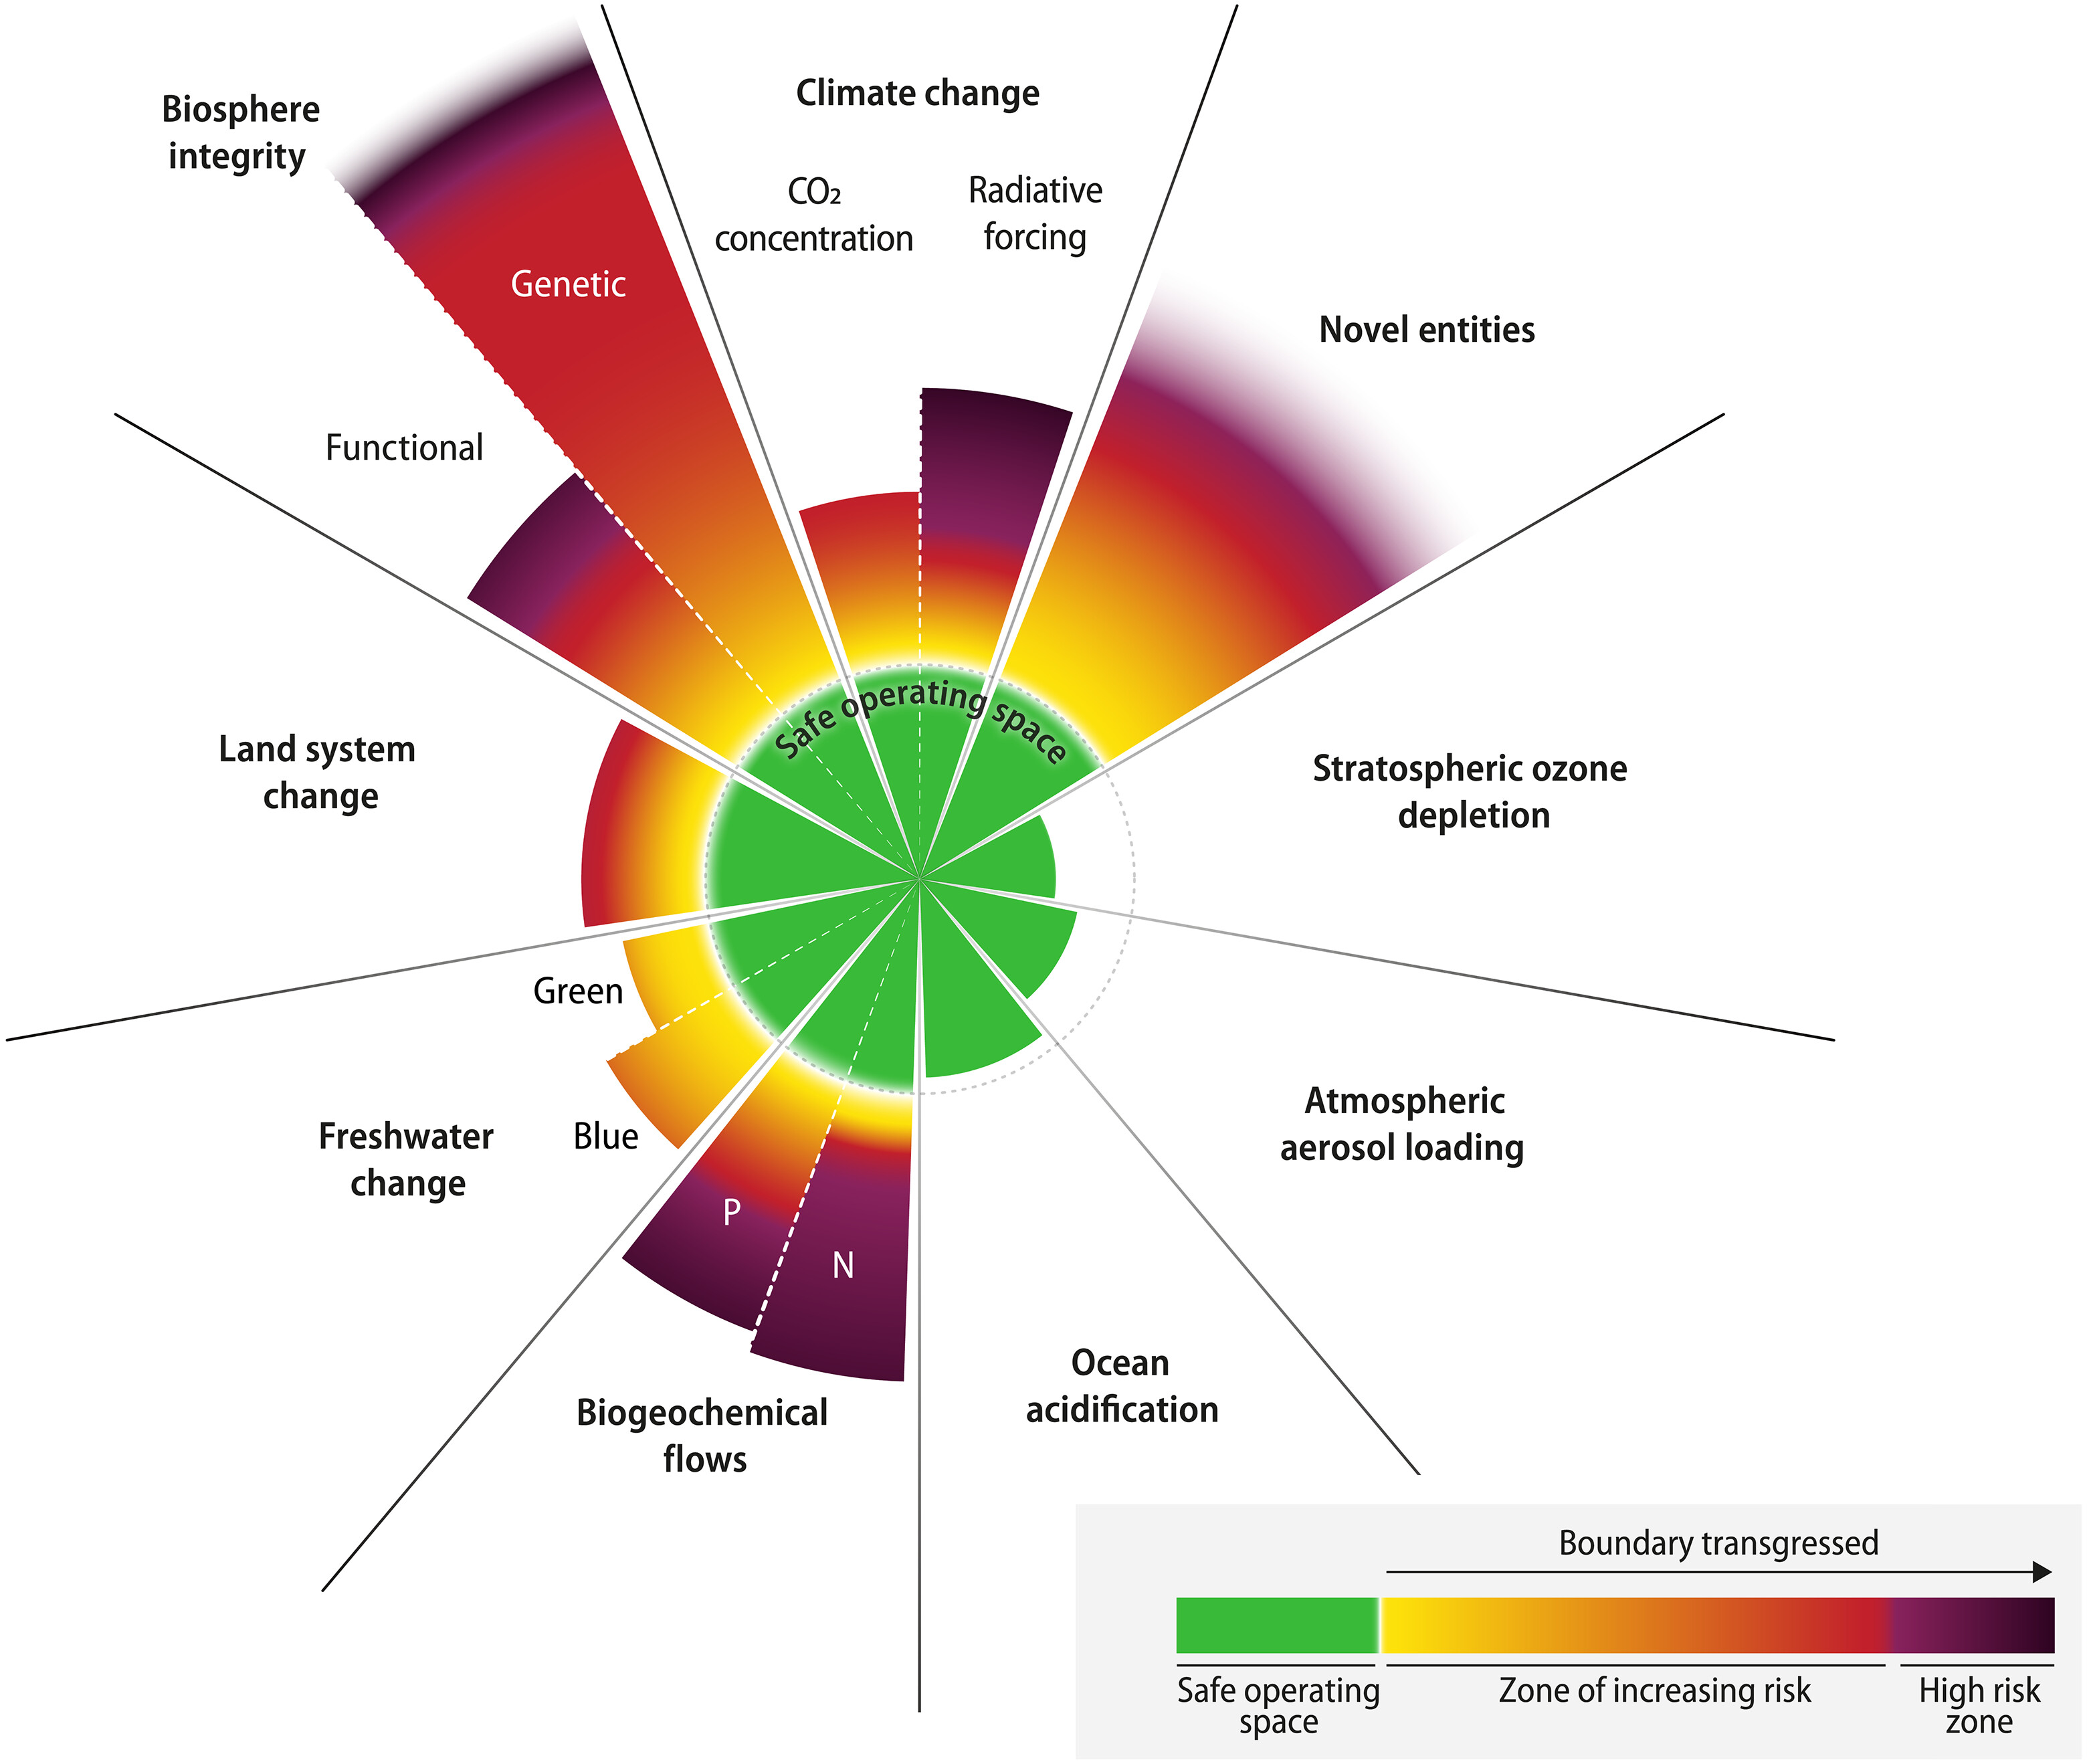
\includegraphics[width= .7\textwidth]{figures/intro/planetary_bounds.jpg}
	\caption{Current status of control variables for all nine planetary boundaries, from \cite{richardson_earth_2023}}
\end{figure}

Among these planetary limits, the integrity of the biosphere has gradually become of particular interest, along with its interaction with other limits, such as climate change, or novel entities (including pollution). Created in 2012, the Interdisciplinary Panel on Biodiversity and Ecosystem Services (IPBES) has been raising the alarm on the state of "Nature" globally. Its chair, Sir Robert Watson, put it clearly\footnote{See the \href{https://www.ipbes.net/news/Media-Release-Global-Assessment}{press release address of the 2019 report}}:
\begin{displayquote}
"\textit{The overwhelming evidence of the \cite{ipbes_2022_6417333} Global Assessment from a wide range of different fields of knowledge, presents an ominous picture [...]. The health of ecosystems on which we and other species depend is deterioriating more rapidly than ever. We are eroding the foundations of our economies, livelihoods, food security, health and quality of life worldwide}"
\end{displayquote}

"Nature" is a central concept in the IPBES framework \citep{ipbes_2022_6417333}:

\begin{displayquote}
\textit{Nature (also defined as living nature) [is] the nonhuman world, including coproduced features, with particular emphasis on living organisms, their diversity, their interactions among themselves, and with their abiotic environment. Within the framing of natural sciences, nature includes e.g. all dimensions of biodiversity, species, genotypes, populations, ecosystems, the biosphere, ecosystem functioning, communities, biomes, Earth life support's systems and their asosicated ecological, evolutionary, biogeochemical processes and biocultural diversity. Within the framework of economics, it includes categories such as biotic natural resources, natural capital, and natural assets. Within a wider context of social sciences and humanities and interdisciplinary environmental sciences, it is referred to with categories such as natural heritage, living environment, or the nonhuman. Within the context of other knowledge systems, it includes categories such as Mother Earth [...], Pachammama [...]}\\
\hspace*{\fill} \small{\cite{ipbes_2022_6417333}, p.14, see also \cite{DIAZ20151}}
\end{displayquote}

Nature, as defined in this approach, is a very large and complex object.
It is defined across ontological and epistemological differences (living and non-living e.g. matter), different types of interactions, at various scales (genotypes v. ecosystems), at different types of processes (biological v. ecological), and across different fields of inquiry (natural sciences v. social sciences). In this dissertation, I study more specifically "biodiversity", which focuses on the variability among living organisms. While it is itself an ambiguous concept, biodiversity tends to put the focus on living organisms, in relation to their material, biotic and abiotic environment (as opposed to the study of the non-living environment) and on its critical role among other components of the Earth system.

The \cite{ipbes_2022_6417333} report documents the drastic changes the biosphere is going through and considers these changes through an \textit{anthropocentric} lense, e.g. mediating the aforementioned changes through the multiple and diverse contributions that Nature and biodiversity bring to people. It stresses how disruption impacts human lives and highlights the role of anthropogenic (e.g. of human origin) drivers of the disruption of Nature and biodiversity. 
 
This reports sets different objectives to scientific research. The first objective is to explain the feedback mechanisms : how do human livelihoods impact biodiversity? In response, how does biodiversity impact human livelihoods? This objective involves understanding the causes and measuring the direct and indirect anthropogenic drivers of change in Nature and biodiversity on the one hand, and on the other hand understanding the channels and scales through which Nature and biodiversity contribute to human livelihoods, as well as measuring these contributions. Hence, studying the demise of nature, and the potential to remedy it calls for an integrated perspective, that joins natural sciences to social sciences, through frameworks such as social-ecological systems \citep{Ostrom2009}. 
\\
The second objective is to provide a framework to assess the desirability, the feasibility and means of implementation of collective pathways that would remedy the crisis nature is facing. In a way, it involves designing and implementing policy pathways towards sustainable futures, e.g. finding definite courses or methods of action selected from alternatives, at the individual, collective or governmental levels, to achieve future states of the world which remain in a safe operating space regarding planetary bounds \citep{rockstrom2009safe,steffen_2015_planetary}.

In this dissertation, I take on these two objectives using a framework stemming from economics and ecology. A first version of the research questions this thesis aims at solving is: 
\begin{enumerate}
\setlength{\itemsep}{0pt} % No space between items
\item What are the feedback relationships between biodiversity and antropogenic drivers of its decline? 
\item What underlying mechanisms must policy pathways tackle to remedy this demise?
\item  How can integrated economic and ecological approaches be used and refined to analyze inform and design policies? 
\end{enumerate}

In order to refine these questions, I first define the concept of biodiversity, through its natural and social sciences appraisals, and highlight ongoing trends in its demise.


\subsection*{Emergence and definition of biodiversity as an ecological concept}
\addcontentsline{toc}{section}{Emergence and definition of biodiversity as an ecological concept}

Biodiversity emerged as a concept in the 1980s, along with the emergence of "conservation biology", a branch of biology concerned with the protection of "biological diversity" \citep{soule_what_1985}, as a response to an acceleration in the loss of species, which have intrinsic value, e.g. should be protected for their own sake \citep{soule_conservation_1986}. 
The concept of biodiversity is therefore embedded in an ethical judgement and a call for action. In the wake of the 1992 Rio United Conference on Environment and Development, the Convention on Biological Diversity emerged as an international treaty to safeguard biodiversity. In doing so, it provided an internationally agreed upon definition:

\begin{displayquote}
"\textit{"Biological diversity" means the variability among living organisms from all sources including, inter alia, terrestrial, marine and other aquatic ecosystems and the ecological complexes of which they are part; this includes diversity within species, between species and of ecosystems.}"\\
\hspace*{\fill} \small{\href{https://www.cbd.int/convention/articles/default.shtml?a=cbd-02}{Article 2 of the Convention on Biological Diversity}}
\end{displayquote}

This definition highlights a key differentiating feature from other parts of Nature, e.g. the living nature of the objects of study. Compared to abiotic factors, biological diversity is characterized by intrinsic growth and reproduction rates (at the individual and population levels), and evolution (at the genetic, and species level). Additionally, these rates of change through time are commensurable with human experience, and most processes (e.g. reproduction, population collapse or recovery, genetic evolution) can be observed within a human lifetime as opposed to the geological temporal scale. 

As highlighted by \cite{mouysset_diversity_2023} and \cite{VanDyke2008}, the definition of biodiversity is difficult, as it recovers ethical, conceptual and measurement dimensions. Biodiversity can be viewed as "an intrinsic, value-ladden quality of natural systems that should be preserved for its own sake" \citep{VanDyke2008, mouysset_diversity_2023}, but it also refers to measurable features
% relevant to understanding genetic distribution, population levels, community structure (e.g assembly of interacting species in a given area), environmental processes, and ecosystem functions (e.g. the ecological processes performed by living organisms, such as carbon sequestration, nutrient recycling, water filtration etc). 

This definition implies different scales from a hierarchical perspective, at the genetic level, at the species, the community, and the ecosystem levels (defined as the interaction of communities and their abiotic environment). These levels imply different forms of measurement, including the distribution of genes, species abundance (e.g. the number of individuals in a population, at a given time and location), species richness (e.g. the number of different species, at a given time and location) within communities, among communities, and across larger scales (e.g. alpha, beta and gamma diversities.), as well as variations in the abiotic factors that form ecosystems, such as temperature, humidity, water quality, soil quality etc. 
It also comprises different types of diversity : structural diversity (for example, the layers of canopy in forests, the sex-ratio in animal populations), compositional diversity (the variety and abundance of species within a community), and functional diversity (variety of environmental processes performed by living organisms in a given area e.g. carbon sequestration, nutrient cycling or seed dispersal, see \cite{loreau_biodiversity_2002})

\begin{figure}
	\centering
	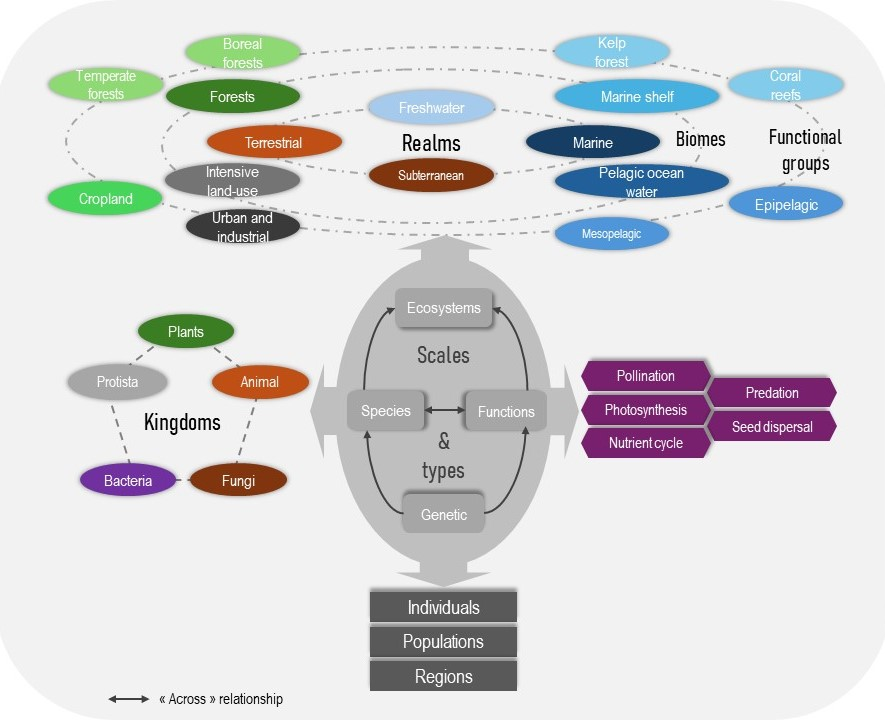
\includegraphics[width =.8\textwidth]{figures/intro/biodiv_illustration.jpg}
	\caption{Biodiversity : a multiform concept across scales and types}
	\label{fig:intro_biod}
\end{figure}

Compared to other subfields of biology,  \cite{mouysset_diversity_2023} highlights the difficulty of articulating the definition with common levels in scientific analysis e.g. genetic, taxonomic, and ecosystem, as biodiversity level can fall in between: " populations may be considered from a genetic and taxonomic perspective, or communities that fall between the taxonomic and ecosystem levels". Additionally, as structural and compositional diversity can be seen as the source of functional diversity, the different classes of diversity may be difficult to work with given their colinearity. 

The multiple dimensions of biodiversity highlight several of its critical features. First, it is impossible to measure biodiversity with a single indicator. The study of biodiversity requires multiple indicators to integrally assess the evolution of biodiversity, across scales and types of diversity. The emergence of the concept responds to a desire to protect biodiversity for its own, but also humanity's sake. 

\subsection*{Nature's Contributions to People: rationales for biodiversity conservation}
\addcontentsline{toc}{section}{Nature's Contributions to People: rationales for biodiversity conservation}

While originally descriptive, ecosystem functions have gradually been referred to from the human point of view (starting in the 1970s, see  \cite{hueting1969functions, schumacher1973small}) and how these functions served human societies, through the concept of \textit{ecosystem services} \citep{ehrlich1981extinction}, as a pedagogical tool to illustrate the consequences of biodiversity loss \citep{gomez_history_2010}.  In this respect, a value switch was operated from an intrinsic value towards an anthropocentric value (e.g. given by humans) standpoint \citep{mouysset_diversity_2023}. In more details, biodiversity features an instrumental value (e.g. serves to achieve a human end) and a relational value (e.g. the importance of desirable, meaningful, and often reciprocal relationships - beyond means to an end) : if biodiversity is to be preserved, it is because of the functions it performs that sustain and improve human life.

The concept gradually gained traction in academic research, and as \cite{Costanza1997} quantified the value of natural capital and ecosystem services, at a staggering 33 trilion \$USD, amounting to approximately 30\% of the 2020 World GDP, the concept reached the policy arena. In 2003, the Millenium Ecosystem Assessment \citep{MEA2005} placed ecosystem services at the center of the policy agenda : it emphasized an anthropocentric value of ecosystem services, but established a dependence of human societies on ecosystem services, and further, on the functioning of ecosystem. In this respect, the Millenium Ecosystem Assessment \cite{MEA2005} was a landmark in safeguarding biodiversity through a \textit{strong sustainability} paradigm (see box 1), and triggered the operationalization of the concept into policy at a large scale (which I will develop later on). The ecosystem services framework was divided into 4 categories, relating to the specific type of services contributing to "human wellbeing" : supporting services (e.g. services allowing for other ecosystem services to be present, including nutrient cycling and primary production) and regulating services ("benefits obtained from the regulation of ecosystem processes" e.g pollination, waste decomposition etc); cultural services ("the nonmaterial benefits people obtain from ecosystems through spiritual enrichment, cognitive development") and provisioning services ("all the products obtained from ecosystems"(\cite{MEA2005}, p.54)

\begin{figure}[h]
	\centering
	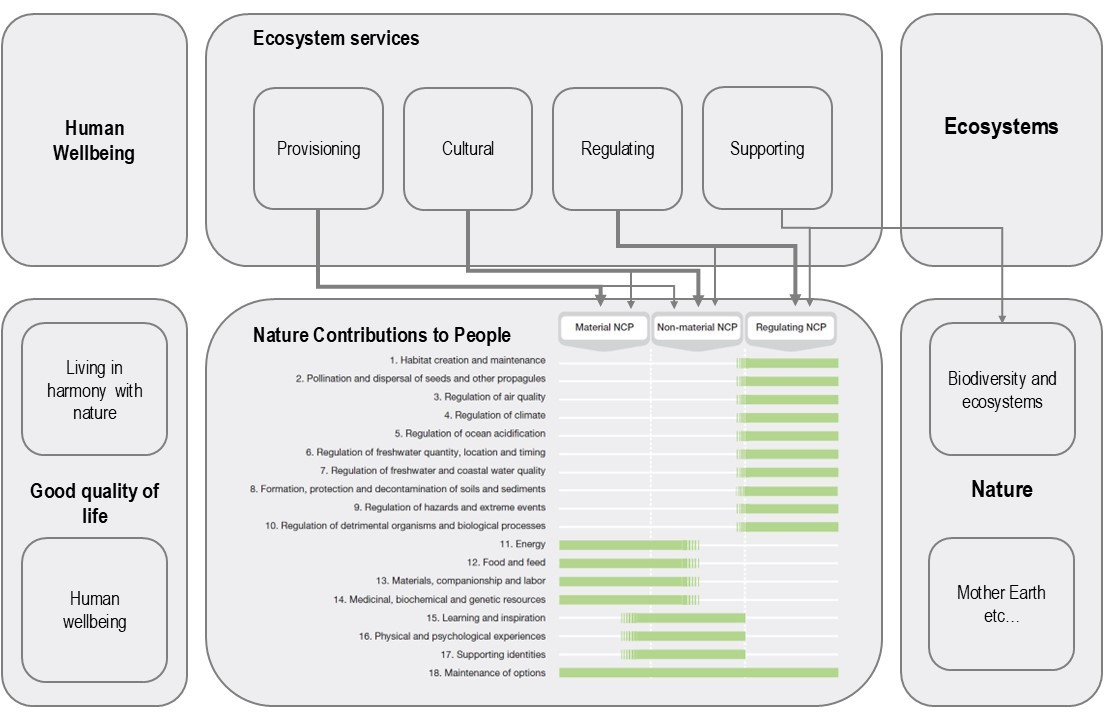
\includegraphics[width = \textwidth]{figures/intro/NCPs2.jpg}
	\caption{Description of the 18 Nature Contribution to People and the connection between the NCP framework \citep{ipbes_2022_6417333} and the Ecosystem Services Framework \citep{millennium2005ecosystems}}
	\subcaption*{Adapted from \cite{diaz_2018} and \cite{ipbes_2022_6417333}}
\end{figure}

Recently, the IPBES platform moved onto a new conceptual framework highlighting Nature Contributions to People (NCP) \citep{DIAZ20151}, defined as "all the contributions, positive and negative, of living nature [...] to people's quality of life \citep{diaz_2018}". This framework underpins 3 types of contributions to people: material contributions to people (flows from nature to people typically consumed to "operate a society or enterprise" (IPBES, p.16), non material contributions (eg. nature's effects on "subjective and psychologica aspects underpinning peoples quality of life) and regulating contributions (e.g. "functional and strcutrual aspects of organisms and ecosystems that modify the environmental conditions experienced by people and/or regulate the generation of material and non material contributions"). This framework highlights how Nature Contributions to People can be positive or negative, and depend on the spatial and temporal definition of the contribution, as a given entity can be at the same time the source of positive and negative contributions: for example, forests foster habitat, but also risk endangering people in the event of wildfires. Additionally, it provides a more encompassing view than ecosystem services, as it encompasses perspectives ranging from biodiversity as natural capital employed in an ecological production function (see \cite{polasky_integrating_2009} for a review), as well as perspectives where biodiversity has agency and is linked by reciprocal care obligations to humans \citep{descola}. 


\begin{tcolorbox}[breakable, 
colback=verylightgray, 
colframe=gray!75!black, 
title= {Box 1 - Weak v. Strong Sustainability},
%code={\singlespacing},
fontupper=\small]
\par % This \par ensures spacing before the text starts
\justifying % Start justified text

In 1987, the release of the Brundtland Report \citep{brundtland} provided a broad definition of sustainable development: 

\begin{displayquote}
\textit{"In essence, sustainable development is a process of change in which the exploitation of
resources, the direction of investments, the orientation of technological development; and institutional change are all in harmony and enhance both current and future potential to meet human needs and aspirations"}\\
\small{\cite{brundtland}, p.43}
\end{displayquote}

Implementing sustainable development remained an open question. In economics, a "weak sustainability perspective", pioneered by works of \cite{hartwick_intergenerational_1977} and \cite{solow_intergenerational_1986} on exhaustible resources, suggested that "maintaining a non-declining capital stock,which allegedly could be put into practice by investing in manufactured capital all the rents derived from the exploitation of non-renewable natural resources" \citep{gomez_history_2010}. In this approach, natural capital could be integrally substituted by human made capital. On the other hand, the "strong sustainability" approach advocates advocates for a complementarity, rather than substitutability of resources \citep{costanza_daly}, acknowledging the dependence of humans on ecosystems
\end{tcolorbox}

This first section highlights a multifaceted correspondence between the different components and dimensions of biodiversity and its contributions to people. Different scales and dimensions of biodiversity underpin NCPs, essential to human livelihood. The global decline of biodiversity threatens NCPs, calling for policy.

\subsection*{Decline in biodiversity : trends and drivers}
\addcontentsline{toc}{section}{Decline in biodiversity : trends and drivers}

Biodiversity metrics are declinning across all the scales of analysis. The structural conditions of ecosystems, the compositions of ecological communities and populations of species have experienced dramatic changes. The share of unchanged, protected wildlife habitat has plumetted on both land and sea \citep{watson_2016_catastrophic, jones_2018_location} to 23\% and 12\% of space, respectively. At the community level, the share of originally present biodiversity falls bellow 90\% across all biomes, \citep{Hill311787} and local communities are becoming more and more similar \citep{mckinney_1999_biotic}, driven by the increased extent of animal and plant non-alien invasive species, rising by 13\% per decade \citep{seebens_no_2017}. At the species level, to date, global species richness is threatened by a mass extinction, as the global rate of species extinction is at least ten times higher than the average rate over the past 10 million years and is accelerating \citep{barnosky_has_2011, ceballos_accelerated_2015}. On average, 25\% of species are currently threatened with global extinction across a wide range of plant and animal species, on land and at sea \citep{IUCN_redlist_2024}.  Habitat based methods \footnote{ The IUCN Redlist uses detailed accounts for species, in a bottom-up approach, to analyze the extinction risk of species. A top-down approach, relying on the evolution of available habitat and the species-area relationship, uses changes in land use to forecast the extinction of species in a more aggregate manner \citep{Diamond1972BiogeographicKE}}, \cite{Hoskins309377} find that hundreds of thousands of plant and animal species are threatened, and will repay the \textit{extinction debt} caused by anthropogenic changes to their habitats : only 92.1\% of terrestrial vertebrate species, 91.6\% of terrestiral invertebrates and 90.7\% of terrestrial plants have enough habitat to persist. These results suggest that around half a million terrestrial animal and plant species - including over 3000 vertebrates and over 40,000 plants - \textit{dead species walking}, doomed to become extinct, unless their habitats improve in time to prevent it \citep{ipbes_2022_6417333}.

%\begin{figure}[h]
%    \centering
%    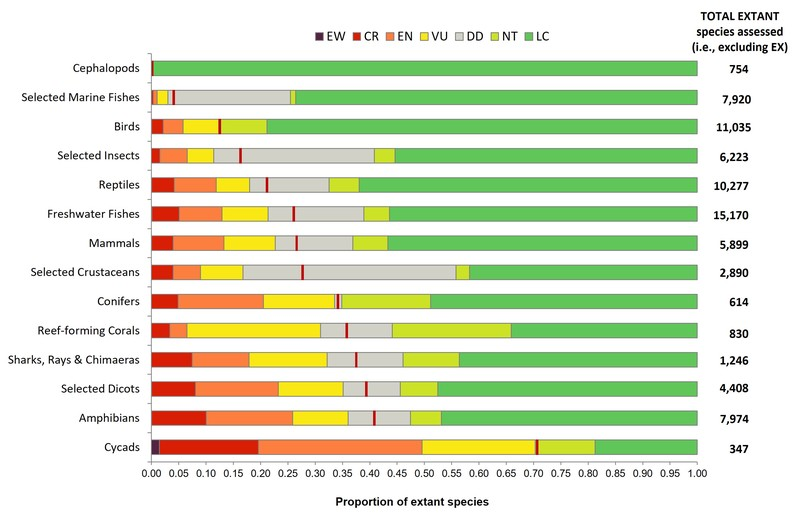
\includegraphics[width=0.8\linewidth]{figures/intro/IUCN_redlist}
%    \caption{The proportion of extant (i.e., excluding Extinct) species in \citet{IUCN_redlist_2024}}
%    \subcaption*{Assessed in each category for the more comprehensively assessed (i.e., at least 80\% of the group has been assessed) groups containing $\geq$ 150 species. Species are grouped into classes. The numbers to the right of each bar represent the total number of extant species assessed for each group. \textbf{EW} - Extinct in the Wild, \textbf{CR} - Critically Endangered,\textbf{ EN} - Endangered, \textbf{VU} - Vulnerable, \textbf{NT} - Near Threatened, \textbf{DD} - Data Deficient, \textbf{LC} - Least Concern.}
%    \label{fig:intro_iucn}
%\end{figure}

Drivers of biodiversity decline are of anthropogenic origin. They can be classified between \textit{direct} drivers, e.g. that directly flow form human actions, such as land use change, anthropogenic climate change, overexploitation, and \textit{indirect} drivers, that can be viewed as the root cause for direct drivers, such as  , changes in the value systems that underpin nature uses (\cite{ipbes_2022_6417333} p.55), demography (urbanization and migration), technology, economy (sectoral transitions, trade expansion) and governance (including risht systems for access to resources).

%The Essential Biodiversity Variables framework \citep{pereira_essential_2013} aggregates fine gridded spatial data into 
A synthesis of natural sciences performed by \cite{ipbes_2022_6417333} outlines the roles of principal drivers at the global scale and across realms (see figure \ref{fig:intro_impacts}).
It shows that land and sea use, reefering to the loss, fragmentation\footnote{Undoubtedly, habitat loss is the main driver of terrestrial biodiversity decline. The effects of fragmentation on biodiversity are highly debated. From a theoretical perspective, models have been developed to study the evolution of populations and communities through space and time, e.g. metapopulation and metacommunity models. Theoretical insights highlight that habitat fragmentation increase the extinction risk, and lower colonization probability, resulting in lower survival and diversity \citep{adler_persistence_1994,hill_habitat_1999, thompson_loss_2017}. At the community scale, increases in diversity among communities (e.g. beta diversity) can emerge from different species resource requirements and the larger spatial extent, hence encompassing more environmental heterogeneity, that results from fragmentation \citep{lasky_reserve_2013, chisholm_species_2018}. However, these effects dampen as habitat loss decreases.  
However, at the empirical level, the effect of fragmentation is highly debated. According to \cite{fahrig_ecological_2017}, there is no empirical evidence that a group of small habitat patches generally has lower evological value than large patches of the same total area. Evidence is however found to show that fragmentation does not reduce habitat connectivity, as functional connectivity is improved (e.g. species are in contact with more different resource patches, thus improving the overall functionning). The debate between \citep{fletcher_is_2018} and \citep{fahrig_habitat_2019} surrounds critics based on the ability of statistical models to encompass the effect of fragmentation when habitat loss is present \citep{ruffell_accounting_2016}. Moreover, it reflects the difficulty of landscape ecology, as different mechanisms across scales e.g. patch, landscape and study region, and measures, such as patch size, patch isolation (e.g. distance across patches) and distance to patch edge (e.g. distance to edge within the patch) interact with possible non-linear interactions.}
%
and degradation of wildlife habitat are responsible for 30\% of the impacts on biodiversity. The direct exploitation of wildlife, wild plants and trees represents 23\% of impacts. Climate change, through shifts in biogeographic conditions and changes in habit, impacts on species traits and genetic evolution represents 14\%, and pollution represents 14\% of impacts. Finally invasive alien species represent 11\%. These drivers have differenciated impacts across ecosystems and biomes \citep{ipbes_2022_6417333}. 

\begin{figure}[h]
	\centering
	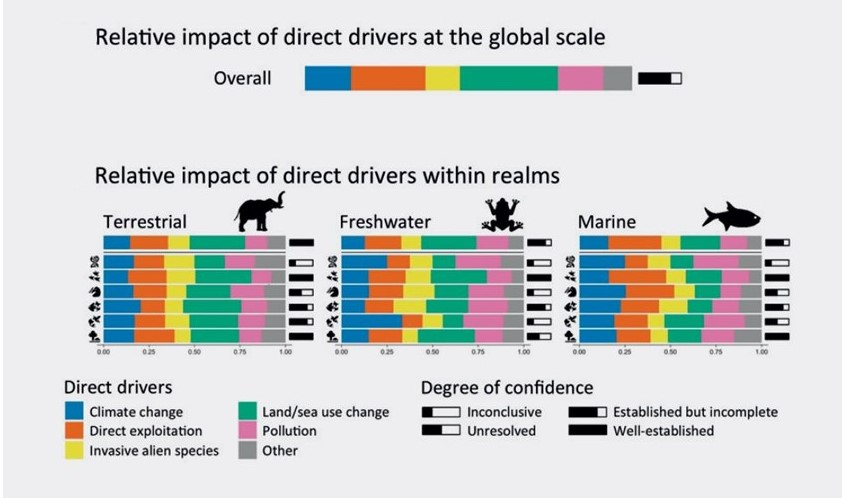
\includegraphics[width = .95 \textwidth]{figures/intro/intro_impactsfin.jpg}
	\caption{Aggregate and realms specific impacts of anthropogenic direct drivers of biodiversity decline adapted from \citep{ipbes_2022_6417333}}
\end{figure}


Land use change is the most important driver (30.5\%), driven by deforestation and agriculture, and direct exploitation follows next (21\%). Tropical and subtropical dry and humid forest host the greatest biological diversity. For example, they host the 10 hotspots with the greatest total number of vertebrates \citep{mittermeier_global_2011}. In such forests, habitat loss and degradation are the main drivers of reductions in species abundance and richness \citep{newbold_global_2014}. Legal and illegal selective logging destroy habitat \citep{hoare2022establishing,  bousfield_2023_large} and are combined with hunting and poaching of wildlife \citep{gallego_2020_combined}, generating between 60 and 180 billions  \$ USD of revenue \citep{gfi_2017}\footnote{Illegal wildlife trade represents between 5 and 23 billion \$USD, while illegal logging represents 52 to 157 billion \$USD}. Mediterranean forests, wooldlands and scrubs, covering 4 million km$^2$, are areas of exceptionally high diversity too \citep{Mooney2001, blondel_2010}. 

For marine species, overexploitation is the main driver (29\%) \citep{ipbes_2022_6417333}. With 90 million tons of capture  (and 141 billion \$ USD)  in 2020 \citep{fao_2022_state}, fisheries stock within biologically sustainable levels have decreased to 64.6\% in 2019, from 90\% in 1974\footnote{ In this calculation, all fishery stocks are equally counted, irrespective of their abundance or catch}, driven by overfishing in the Southeast Pacific and the Mediterranean and Black seas. Assessment of fisheries stock and catch management have been proved to improve livelihoods as well as fish stocks globally \citep{melnychuk_2017_fisheries, hilborn_2020_effective}. Nonetheless, illegal, unreported and unregulated (IUU) fishing is a threat to fisheries. Estimates from 15 years ago \citep{agnew_estimating_2009} estimated it represented between 11 and 26 million tonnes of fis with a value of 10 to 23 billion \$ USD. 
 
Additionally, anthropogenic climate change drives ecosystem disruptions on land \citep{burrell_anthropogenic_2020, conradi_reassessment_2024} and at sea \citep{gomes_marine_2024}, through changes in various channels including ecological suitability and foodweb disturbances. On land, for example, in medditeranean forests,wildfire frequency and severity are expected to increase with global warming \citep{Dupuy2019ClimateCI}, causing important direct and indirect costs to society including destruction of infrastructure and perturbations to economic activity \citep{wang_economic_2021}, smoke related health conditions \citep{burke_wildfire_2023, heft-neal_behavior_2023}, disrupting structural features of ecosystems \citep{Ayars2023} and threatening biological diversity \citep{Wintle2020}.
 
\subsection*{Challenges to remedying the drivers of decline}
\addcontentsline{toc}{section}{Challenges to remedying the drivers of decline}

The anthropogenic nature of the drivers of biodiversity decline suggest that anthropogenic actions can also remedy this decline, through policy design and implementation. This requires finding the relevant obstacles and challenges for each drivers and set a determinate courses of actions, at different organisational levels (individual, collective, state implemented or supranational governance).

Habitat loss and overexploitation present both common and differentiated challenges. A common identifiable cause is the large opportunity cost of preserving a species habitat, or existence, in the presence of other economic alternatives for land and time, as well as financial constraints. Additionally, habitat loss and overexploitation share a temporal dynamic aspect, where immediate actions have durable consequences, possibly irreversible.

Habitat loss and fragmentation in terrestrial ecosystems present specific challenges. Forests, for example, serve multiple uses (or NCPs) by various agents: loggers profit from timber, settlers clear land for agriculture, hikers seek pristine landscapes, and conservationists aim to restore natural cycles. Forests also hold spiritual and cultural value, creating conflicts among these uses. For instance, deforestation destroys both habitat and sacred land, while wildfire prevention can damage wildlife habitat. Species can also have mixed impacts; deer, for example, are valued at low densities but cause damage at higher densities \citep{putman_identifying_2011}. Climate change worsens habitat loss by altering habitat distribution and increasing threats like wildfires \citep{Dupuy2019ClimateCI,wasserman_climate_2023}\\
A second key feature to halt habitat fragmentation is considering the integral set of interdependencies, ecological spillovers and economic externalities that underlie the spatial dimension. The configuration of space, and species movement is at least partly the result of an economic decision. Maintaining habitat connectivity involves identifying patches and paths to be conserved or restored that contribute most to it, in the form of corridors, ecoducts or stepping stones \citep{Turner2005, Turner2011}. The value of patches and paths for connectivity is intrinsically linked to their surrounding : at the same geographic location, a patch has differential value for biodiversity habitat if it is connected to others, or if it is isolated (see box 3). When paths are beyond human control, patches have different importance based on their location, and when the location of patches is fixed, the extent of paths and their location is paramount.
\\
Third, as multiple actions and uses structure connected elements of ecosystems (e.g. different tracts of land, or different biodiversity scales), they trigger spatial spillovers e.g. consequences that go beyond their \textit{in situ} effects. When these spillovers are not taken into account by the agents that generate them, they can be called "dynamic spatial externalities" \citep{sanchirico_bioeconomics_1999, costello_optimal_2008, costello_private_2017}. As halting habitat loss and fragmentation involves conserving tracts of land, neighboring parties may very well benefit (or suffer) from more wildlife and ecosystem (dis-)services on their property, through time. These externalities can trigger specific problems of "race to the bottom" \citep{costello_private_2017} : when neighboring parties of a decision maker that undertakes conservation, or risk reduction, fail fail to reciprocate as they benefit from spillovers, a vicious circle of least action is triggered. Conversely, when ecological spillovers are positive, this may lead everybody to use a resource at unsustainable levels \citep{costello_optimal_2008}. Hence, habitat fragmentation and overexploitation are interrelated through spatial connectivity. 
\\
Fourth, improving habitat loss and fragmentation involves coordinating numerous actors towards increasing the area and connectivity of habitat, while taking into account the associated costs and benefits. In some cases, the financial constraints, the magnitude of costs associated with increased habitat connectivity and the difficulty of coordination warrant a public policy where a central planner undertakes the action \citep{Mouysset2012}, but studying decentralized mechanisms, where individuals undertake incentivized actions, are a worth investigating. 
	 
%\textbf{Peut être à bouger dans les politiquess}	 
%	 ; for pests\footnote{For example, the \href{https://www.nrcs.usda.gov/group/143/feral-swine-eradication-and-control-pilot-program}{Feral Swine Eradication and Control Pilot Program} in the US, helped landowners to eradicate feral swines, to restore ecosystems and to change the potential movement of feral swines through landscapes, with fences and traps}, local targeted incentives to control the population and dispersal can have far reaching consequences, if properly targeted. 
	 
	 
%	. As habitat is altered, so is the surrounding matrix, which can impede species movement \citep{eycott_meta-analysis_2012, kuefler_conflicting_2010} and alter evolution and selective regimes \citep{cheptou_adaptation_2017}.  
\clearpage
\begin{tcolorbox}[breakable, 
colback =verylightgray, 
colframe=gray!75!black,
title={Box 2 - Habitat Loss, Fragmentation and Connectivity},
%code={\singlespacing},
fontupper=\small]
\label{box:policy_frameworks_for_biodiv}


\par % This \par ensures spacing before the text starts
\justifying % Start justified text

Habitat loss refers to the loss of areas featuring suitable environmental conditions for species survival and development. At a constant habitat area, fragmentation refers to increases in the number of patches and decrease in the mean size area of each patches, as in figure \ref{fig:connectivity_intro}. \\
Landscape connectivity is defined in relation to fragmentation. It measures "the degree to which the landscape facilitates or impedes movement among resource patches" \citep{taylor_connectivity_1993}. 
It recovers a \textit{structural} dimension, which describes the physical arrangements across patch and a \textit{functional} dimension, which emphasizes the ability and realization of movements of individuals through the landscape.

 Aggregate connectivity measures take into account the role of differentiated patches and paths. In panel D of figure \ref{fig:connectivity_intro}, the circled patch plays an instrumental role in maintaining connectivity. Habitat patch 1 and 2 have the same number of connected patches. However, patch 1 is maintains the connection between the east and west habitat patches in the landscape, and is connected to highly connected patches. Removing habitat patches 1 and 2 would have larger consequences on habitat consequences than removing other identical size patches. Similarly, removing the dotted path (bottom left of panel D) would isolate patch 3, while removing the dashed path would not leave patch 4 isolated. Hence, paths and patches have different impacts on connectivity, depending on the surrounding patches and paths.
\\% Adds some space before the image
\begin{center}
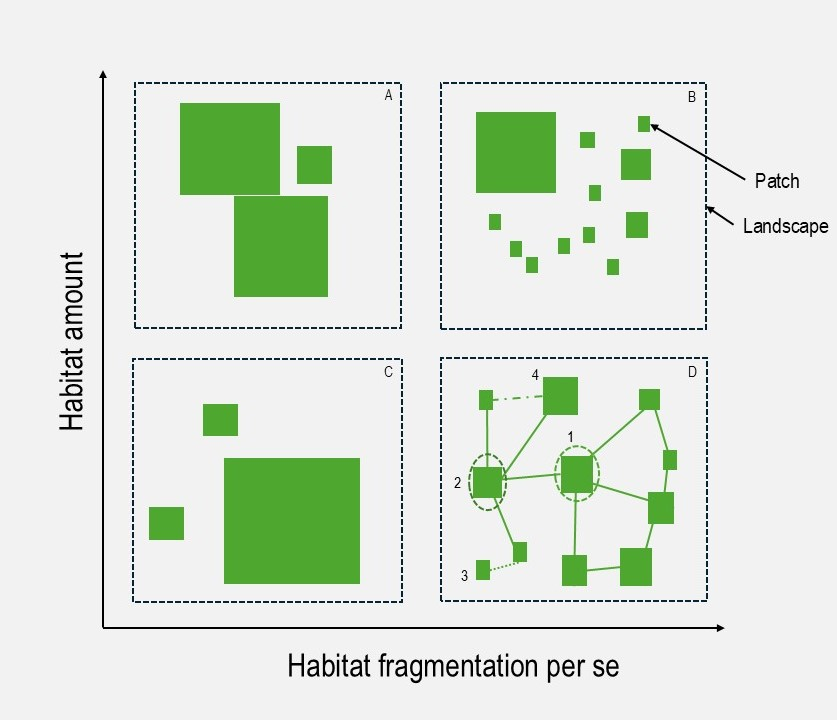
\includegraphics[width = .8\textwidth]{figures/intro/fragmentation.jpg}
\captionof{figure}{Illustration of the effects of habitat loss and fragmentation, adapted from \cite{fahrig_habitat_2019}, and of connectivity}
\label{fig:connectivity_intro}
\end{center}


\end{tcolorbox}

	Halting overexploitation requires understanding and addressing its motives. Overexploitation (or under control, for pests), results from an imbalance between the appropriation and incumbance of Nature's contributions to people (both positive and negative) and the socially desirable level and allocation of these contributions. 	
	The common nature of most natural resources \citep{Gordon1954, smith_models_1969} has long been identified as one of key reason for their demise: numerous events have shown a "race to the bottom", where the absence of secure property rights hastened the overharvest and decline of populations. It has long been the center of attention, and mechanisms to assign property rights have been studied extensively (\textbf{references}). However, while property rights may be assigned, they can be notoriously hard to enforce in areas where regal functions are challenged: \textit{de facto} rights are assigned and enforced. In this case, the common nature of the resource may not be the main concern: local market concentration forces may outweigh overexploitation forces, even in the presence of some of form of open access \citep{damania_economics_2007}. 
Around the world, wildlife poaching and trade typically originates from organised crime groups, and is associated with different criminal activities \citep{mozer_introduction_2023}.  In those cases, concentrated markets tend to emerge and characterize wildlife markets, as competition is hindered by violent organised crime groups. At one extreme, locally monopolistic markets structure for wildlife products may emerge, especially in the case of endemic species (e.g. native and restricted to an area).
They may  be the conservationists' bestfriend \citep{solow_resources_1974, hannesson_note_1983}, depending on specific, context dependent market and species characteristics, as a monopolist has an interest in restricting supply to increase prices, if consumers do not react too much (e.g. under limited demand elasticity). A vast range of  market structures \citep{damania_economics_2007, hannesson_effects_1985} sticking to real world situations have been studied. However, the full range of interactions between a species endemism, local power and harvest structure and access to final consumer markets require more analysis to clarify the impact of market structure.
	Other drivers of overexploitation can be found in the large expected benefits (relative to other local economic activity) some natural resources can bear, most of the time because of their rarity (e.g. absence of economically viable substitute), whether today or in the future \citep{Kremer2000}. While the effects of substituting man-made products to disrupted ecosystem services are starting to get empirically studied \citep{frank_economic_2024} and show how dreadful costs can be, the effect of introducing substitutes to illegally poached wildlife products can be an example of strong substitutability between natural and man-made assets \citep{chen_economics_2017}. As broader forces affect overexploitation, including poverty, it is clear that adressing overexploitation implies generalizing conclusion from the interplay of a single species with the institutional setting, how a  species' future interacts with the availability of substitutes, and how the distribution of revenues from sustainable harvests may foster a reasoned use of the resource. 
	
	A wide range of policies have been implemented at different organisational levels, to jointly or separately halt the identifed drivers of biodiversity decline on land and at sea, with varying degrees of success. 
 
\subsection*{Policies for remedying the decline}
\addcontentsline{toc}{section}{Policies for remedying the decline}
\par

Successive international policy frameworks have sought to halt biodiversity loss by addressing its drivers comprehensively. In 2022, the 15th conference of the UN Convention on Biological Diversity launched the \href{https://www.cbd.int/doc/c/e6d3/cd1d/daf663719a03902a9b116c34/cop-15-l-25-en.pdf}{Keunming Montreal Global Biodiversity Framework (GBF)}, replacing the Strategic Plan for Biodiversity 2011-2020 and the Aichi Targets. The GBF sets four global goals for 2050, with 23 measurable targets to halt biodiversity loss by 2030. These goals include maintaining ecosystem integrity and connectivity and preventing human-induced extinctions (Goal A), sustainably using biodiversity (Goal B), sharing conservation benefits and burdens equitably (Goals C and D)\footnote{See \href{https://www.cbd.int/doc/c/e6d3/cd1d/daf663719a03902a9b116c34/cop-15-l-25-en.pdf}{Section G. Kunming-Montreal Global Goals for 2050}}. \href{https://www.cbd.int/gbf/targets/5}{Targets} include restoring 30\% of degraded ecosystems, conserving 30\% of land and sea areas, and ensuring the sustainable use and management of wild species.



%\begin{tcolorbox}[breakable, 
%colback=verylightgray, 
%colframe=gray!75!black,
%title={Box 3 - The Convention on Biological Diversity and the Aichi Targets},
%code={\singlespacing},
%fontupper=\small]
%\label{box:policy_frameworks_for_biodiv}
%\par % This \par ensures spacing before the text starts
%\justifying % Start justified text

%In 2010, the Convention on Biological Diversity set its "Strategic Plan for Biodiversity 2011-2020", structured around the 20 Aichi Biodiversity Targets, spanning over 5 goals :

%\begin{itemize}
%\item Goal A : Address the underlying causes of biodiversity loss by mainstreaming biodiversity across government and society
%\item Goal B : Reduce the direct pressures on biodiversity and promote sustainable use
%\item Goal C : To improve the status of biodiversity by safeguarding ecosystems, species and genetic diversity
%\item Goal D : Enhance the benefits to all from biodiversity and ecosystem services
%\item Goal E : Enhance implementation through participatory planning, knowledge management and capacity building
%\end{itemize}

%In 2020, the Global Biodiversity Outlook 5 \citep{global_biodiversity_outlook} showed that none of the Aichi %Target were globally met, and only 6 targets were partially achieved, including the identification and eradication of invasive species on islands, the setting of 17\% of terrestrial and inland water areas and 10\% of coastal and marine areas as conservation areas, the implementation of policy instruments and effective national biodiversity strategy and planning, and the increase in financing biodiversity protection. 

%While several elements showed progress, the failure of the 2011-2020 Strategic Plan was patent. Measurable indicators to assess progress towards targets were missing. This was tackled with the new Global Biodiversity Framework that took over in 2020, although with severe limitations. According to critics \citep{maron_setting_2021}, the current framework also lacks ecological scale-specific indicators (for genes, species, ecosystems) and do not provide specific net outcome statements (such as the 1.5C degree target of the Paris Agreements) across areas, nor a clear implementation timeline. 

%Additionally, the 2011-2020 Strategic Plan failed as countries did not have to report on their progress, only declare their targets. The 2020 Global Biodiversity Framework has implemented follow-up measures : although it is not a legally binding frameworks, countries who have signed commit to demonstrating progress towards the targets and update their National Biodiversity Strategy and Action Plans (see section B.5 and section J of the \href{https://www.cbd.int/doc/decisions/cop-15/cop-15-dec-04-en.pdf}{GBF})
%\end{tcolorbox}
Other international treaties, such as the \href{https://cites.org/fra}{Convention on International Trade in Endangered Species (CITES)} established in 1973, regulate trade in endangered species to prevent illegal wildlife trade\footnote{CITES features 183 member parties (countries), it lists species across "appendices", with varying degree of protection of the species and restrictions limiting the trade in endangered species.\\
Appendix 1 : the most endangered species, threatened with extinction and prohibited international trade, except when the purpose of exports is not commercial\\
Appendix 2 : species that are not necessarily now threatened with extinction but that may become so unless trade is closely controlled\\
Apppendix 3 : species included at the request of a Party that already regulates trade in the species and that needs the cooperation of other countries to prevent unsustainable or illegal exploitation} and promote species survival. Despite its scope, CITES’ effectiveness is debated. Local enforcement \citep{HEID2023102784} and demand reduction campaigns \citep{macfarlane_reducing_2022, moorhouse_demand_2024} are critical, but trade bans can sometimes increase prices and poaching incentives \citep{hsiang_does_2016}. In some cases, conservation farming has succeeded by “flooding the market” \citep{gentry_looking_2019, phelps_framework_2014, tensen_under_2016}. Supply-side interventions have occasionally succeeded at reducing poaching and recovering wild populations – e.g., vicuña and spotted cat \citep{iucn_world_2000, sahley_biological_2007} – but they have also failed – e.g., green python, African elephant \citep{lyons_wildlife_2011, hsiang_does_2016}. Uncertainty around conservation outcomes from market-based approaches has led to continued reliance on trade bans and controls that are often ineffective at reducing poaching.

National and supranational policies have also been key. In the U.S., policies like  \href{https://www.fs.usda.gov/Internet/FSE_DOCUMENTS/fseprd645666.pdf}{Wilderness Act of 1964} created protected areas to preserve habitats. In the wake of the environmentalist movement of the 1960s and 1970s, landmark regulations aimed at protecting natural habitats, such as the \href{https://www.epa.gov/laws-regulations/summary-clean-water-act}{Clean Water Act of 1972} (ensuring sewage to limit the disruption of wildlife habitat), and specifically targeted towards species conservation with the \href{https://www.fws.gov/sites/default/files/documents/endangered-species-act-accessible.pdf}{Endangered Species Act of 1973}. Results of the Endangered Species Act are debated. While the impacts seem to be overall positive on species recovery, budget dedicated to listings are slim , and the associated costs are substantial and concentrated on private landowners while benefits are more broadly distributed \citep{brown_economics_1998, langpap_economics_2018}
%
Localized initiatives, such as the \href{https://y2y.net/}{Yellowstone Yukon Conservation Initiative} (1993), connect ecological areas across the U.S. and Canada,using private conservation and local policy making. 
%
In Europe, the Natura 2000 network\footnote{A system of protected areas, established in application of the European Union Birds Directive (1976) and Habitats Directive (1992), and formally in place starting the mid 2000s} has created the largest conservation area globally, covering 18\% of land and 9\% of marine regions in the EU, across 28,000 sites. In broad strokes, it delineates conservation areas of ecological interest where development and human activities are restricted. Its ambition stemmed from taking into account the scale of biodiversity processes rather than administrative boundaries to develop an interconnected network of conservation areas. The ecological and economic performances of such a network are substantial, as they generate spatial spillovers both in terms of economic and ecological performance \citep{cocco_relaxing_2023}.

Acknowledging that biodiversity habitat can be seen as a continuum between unsuitable and suitable conditions, mechanisms such as Payments for Ecosystem Services (PES) are leveraged to incentivize conservation on agricultural land. Taking into account the ecological spillovers of decreased spillovers, payments for ecosystem services with agglomeration bonuses, such that neighbors gain an additional marginal benefit when a new local participant implements conservation measures, can be efficient \citep{parkhurst2002agglomeration, bareille_agglomeration_2023}. Overall, the spatial consequences of decentralized policies has yet to be fully integrated in policy making.

Finally, some policies aim at mitigating the threats posed by climate change on ecosystems and species, by changing landscape connectivity. In mediterranean forests, where biodiversity is exceptionally high but wildfires are an ever growing threat \citep{Dupuy2019ClimateCI, wasserman_climate_2023}, fuel treatment operations\footnote{Mechanical thinning, prescribed burns, and sometimes, logging, have been leveraged to decrease the fuel load in risky areas and theoretically decrease the probability and severity of burns upon wildfire occurence. In numerous regions, such as conifer forests in California \citep{Vaillant2009, Kalies2016, low_shaded_2023}, eucalypt forests in South Western Australia \citep{burrows2013, boer_long-term_2009, Florec2020}, southern Europe \citep{Fernandes2013}, evidence shows that fuel treatments, can mitigate wildfire intensity and spread. Land management agencies have historically implemented these policies in Australia \citep{burrows2013}, Europe, and the United States (and are projected to ramp up, for example under the Infrastructure Investment and Jobs Act of 2021 in the US)} limit the occurence and severity of wildfires. Public policy is leveraged in the face of increasing risk, limited insurability and threats to biodiversity. For example, with limited insurability of homes in the wildland urban interface in California\footnote{For example, \href{https://www.washingtonpost.com/climate-environment/2024/08/29/california-insurance-wildfires-allstate/}{200,000 homeowners will see an increase in their insurance premium} by an average of 34.1\% from Allstate insurance in November 2024. In 2023, the FAIR plan, designed to be the insurer of last resort in California (state mandated but privately funded) saw a \href{https://www.cfpnet.com/key-statistics-data/}{38.3\% increase in its total exposure.}}, as well as the potential economy-wide human and non-human damages from wildfires \citep{wang_economic_2021, heft-neal_behavior_2023, Ayars2023} state-mandated and operated fuel treatment policies are of the essence. However, with increased budgets and improved spatial planning, these policies could achieve better performances in reducing risk while protecting biodiversity.\\
Decentralized policy mechanisms exist, such as mandates to create a defensible buffer around individual properties : in California, a 100-foot defensible around houses is mandated in State Responsibility Areas,and can translate in reduced insurance premia;  in France, in dedicated regions, the "obligation de débroussaillement" mandates fuel control operations in a 50m radius to "decrease the intensity of wildfires and limit their spread"
\footnote{Translated by the author - \href{https://www.legifrance.gouv.fr/codes/article_lc/LEGIARTI000047809197}{Article L131-10} of the Code Forestier} with fines reaching $5,000$ euros for failing to comply.


I focus on the analysis of the interplay between biodiversity and human actions, through the NCPs it provides and the anthropogenic drivers of its decline. As existing policies have had varying degrees of success in halting biodiversity decline, a framework for policy design is required. I use \textit{economics} to jointly analyze the causes of this decline and offer policy recommendations. 


\subsection*{Biodiversity as an economic object}
\addcontentsline{toc}{section}{Biodiversity as an economic object}

Biodiversity, through its different scales, has a longstanding history as an economic object : hunting, fishing, logging have always been instrumental in human livelihoods and became economic objects to be traded. A long tradition has analyzed the specific markets for so-called renewable resources, e.g. whose natural rate of regeneration is commensurable with human experience, as products with an established market price. In doing so, it only considered said resources through a particular ontological state : dead. Focusing on a single species, this approach was only able to elicit the part of the "use value" of species (see \cite{Krutilla1967} and in the modern NCP framework, the material NCPs associated with food and materials) and not the integral value of species \citep{Krutilla1967}. The notion of "use value" had to be broadened to encompass the direct and indirect contributions of species, through a variety of techniques, and put a monetary value on them. To put a price on biodiversity, a wealth of research has relied on market proxies. On the one hand, hedonic methods \citep{rosen_hedonic_1974} have used the variation in observed market prices for a variety of goods, such as real estate, related to the variation of environmental and biodiversity features, and have studied how these variations have been internalized in goods market prices. On the other hand, methods such as the travel cost method \citep{clawson_economics_1967, bhandari_willingness_2010} have relied on observed consumer behavior and expenditures to experience "Nature", such as wildlife seeing, to elicit the price people are willing to pay for biodiversity. When impossible to apply, for lack of proxy or data, other methods have relied on non-market valuation techniques \citep{carson_contingent_2012}. For example, in 1989, the tanker Exxon-Valdez spilled close to 42 million liters of oil in Alaska, in an ecologically sensitive area : marine populations were decimated\footnote{According to \href{https://darrp.noaa.gov/oil-spills/exxon-valdez}{the National Oceanic and Atmospheric Administration}, an estimated 250,000 seabirds were killed, 2,800 sea otters, 22 killer whales, billions of salmons were killed. Numerous species are not in recovery after 25 years}. In order to hold Exxon accountable, surveys were developped to assess the value of marine biodiversity, by surveying the willingness of people to pay for wildlife\citep{carson_contingent_1992, arrow_report_1993, carson_contingent_2003}, with controversed success \citep{Diamond94}. This strand of work pinnacled with \cite{Costanza1997}. In recent years, these approaches have been further developed by departing from direct monetary metrics, towards measuring the influence of species on other outcomes such as health \citep{frank_social_nodate,frank_economic_2024}. Overall, a variety of methods has been leveraged to extend the valuation of biodiversity at different scales, ranging from genetics to habitats, and encompassing functions \citep{bartkowski_capturing_2015}

With the recognition of its economic value, biodiversity indeed became an economic object, which can be subject to direct monetary valuation, although it raises critics. However, this is not sufficient for biodiveristy and its components to become an actual economic\textbf{s} object. While a definition of economics is made difficult with the recent extension of its objects and methods, it is overall concerned with the analysis of human behavior, at the individual and collective level, to manage scarce resources \citep{mankiw_principles_2011, bade_foundations_2002,backhouse_retrospectives_2009}.\\
Key elements in this defnition are \textit{management}, \textit{resource }and \textit{scarcity}. As management requires a commensurability of objects in terms of values (not necessarily with the same indicators, but a basis for rational comparison), it involves weighing opportunities pertaining to different allocations of a resource, as the available amounts are limited e.g. scarce. In the case of biodiversity, at all scales and across types, this implies considering a specific scarcity, as regeneration rates are commensurable with human experience, and potentially, depletion rates. From an epistemological standpoint, this implies considering the temporal dimension of the resource. Hence, while valuation techniques are a building block in making the economics of biodiversity, an explicit framework to consider the temporal dynamic of biodiversity and the consequences of different actions on its current and future state is paramount. To do so, economists use models : 

\begin{displayquote}
 "\textit{[...] a story with a specified structure. The structure is given by the logical and mathematical for of a set of postulates, the assumptions of the model. The structure forms an unninterpreted system [...]. The theorems that follow from the postulates tell us things about the structure that may not be apparent from an examination of the postulates alone. Although the term 'model' is often applied to a structure alone, we shall use it in another sense. In economists' use of models, there is always an element of interpretation: the model always tells a story}"\\
\hspace*{\fill} \small{\cite{GibbardVarian} p. 4}
\end{displayquote}

As such, models appear as mediators between theory and the real world \citep{morgan_models_2009}. \cite{varenne_epistemologie_2014} furthers this approach and labels models as facilitators, across multiple dimensions. A non-exhaustive typology of the roles models can play includes (i) a pedagogical role (facilitating communication), (ii) a predictive role (facilitating anticipation), (iii) a heuristic role (facilitating the explanation of a mechanism with a few simple interactions), (iv) prescriptive (facilitating the response to a given problem) and (iv) integrative (facilitating exchanges between disciplines). Models used in economics encompass these functions to guide the management and policy of biodiversity. 


\subsection*{Bioeconomic modeling for the study and management of biodiversity}
\addcontentsline{toc}{section}{Bioeconomic modeling for the study and management of biodiversity}

Bioeconomic models \citep{Gordon1954, smith_models_1969, clark_profit_1973} have emerged from joint efforts by economists and ecologists to manage resources accounting for the specific dynamics of biotic elements \citep{Parent_Mouysset_Missemer_Levrel_2024}. Bioeconomic models are analytical tools that jointly model the feedbacks between components of biodiversity in wild or weakly manageed ecosystems and economic activities, at different levels (e.g micro, mezzo and macro levels). 
Historically, the first bioeconomic models have emerged from population ecology and static economic analysis, to study the management of fisheries. The Gordon-Schaeffer model highlights the evolution of a fish population according to different harvest regimes, and aims at maximizing revenues in equilibrium. It distinguishes effort levels between those providing the maximum economic yield from those providing the maximum sustainable yield (e.g. resulting in the largest fish growth), yielding new policy perspectives: as the maximum sustainable yield effort is larger than the maximal economic yield, the policy target should be the former. Aiming for the maximum economic effort would therefore yield larger fish populations and promote economic efficiency. The original model was later extended to account for transitory dynamics and integrate elements from capital theory, focusing on the dynamic allocation of resources through time \citep{smith_models_1969, clark_profit_1973}. 

\begin{itemize}
\item Switch to land : other models focus on agricultural contexts and model the evolution of pests
\item Summary of first chapter:
\begin{itemize}
\item Bring MEY and MSY on land : the harvesting paradigm, swanson etc
\item Other approach : no longer monetize biodiversity and increase spatial granularity
\end{itemize}

\item Outline the evolution of bioeconomic modeling with economic models (e.g. taking into account risk and multiple players, as well as switching from pure optimality to more "positive" approaches) and ecological modeling
\item Gradual evolution of models to fulfill different functions of modeling or be different types of facilitators
\\
Box on ecological modeling : from population ecology to conservation and restoration ecology; change of scales, models integrate more and more spatial heterogeneity etc. 
\end{itemize}

\begin{tcolorbox}[breakable, 
colback=verylightgray, 
colframe=gray!75!black, 
title= {Box 3 - A brief overview of ecological modeling for biodiversity},
%code={\singlespacing},
fontupper=\small]
\par % This \par ensures spacing before the text starts
\justifying %
Ecology is a branch of biology that studies of the relationships between living organisms and their environment. 

While 


\end{tcolorbox}

\subsection*{Specific bioeconomic modeling challenges in the face of anthropogenic drivers}
\addcontentsline{toc}{section}{Specific bioeconomic modeling challenges in the face of anthropogenic drivers}

\begin{itemize}
\item Modelling challenges from the literature : 
\begin{itemize}
\item Integrate space in optimal management and focus on the role of space as an endogenous variable, not just spatial granularity
\item Take into account the full interplay of uncertainties : risk, uncertainty, how decision makers adapt etc. 
\item Operating a switch from population ecology to broader scale approaches that still integrate the dynamics of species, and not just static distributions with niches etc, such as landscape ecology and restoration ecology further
\item Integrate indigenous knowledge and perspecitves
\item Refine the study of intricate (to define more) market dynamics
\end{itemize}
\item Current challenges posed in relation with the challenges outlined in the conceptual part for remedy of overexploitation and habitat loss/fragmentation
\begin{itemize}
\item Integrating space in decision making : 
\begin{itemize}
\item deal with non convexity of objective function; 
\item Optimization on discrete landscapes : cannot use continuity
\item Dimensionality curse : dynamic programming fails, at least when performed brutely, so need to trade (i) temporal depth of planning, (ii) extent of space and (iii) complexitiy of ecological mechanisms. 
\item 
\end{itemize}
\item Refine the study of dynamics with heterogeneous and strategic players:
\begin{itemize}
\item Integrate more the roles of ecological and economic heterogeneity through land : limited scope for analytical tractability, need to resort to numerical methods
\item Interaction on a same market of different types of actors, with strategic responses : complicated choice variables in terms of game theory, as exploitation and decision over space are related; 
\end{itemize}
\item Need a variety of perspectives for models to be helpful for decision making : integrating both a positive approach (e.g. compare policy scenarios in a second best world) and a normative approach to guide policy. 
\end{itemize}
\end{itemize}

\subsection*{Research questions}
\addcontentsline{toc}{section}{Research questions}

\begin{itemize}
\item Remind the NCPs I'm focusing on :
\begin{itemize}
\item NCP1 - Habitat creation and maintenance : "the formation and continued production, by ecosystems, of ecological conditions necessary or favorable for living beings important to humans"
\item NCP10 - Regulation of organisms detrimental to humans : "regulation, by ecosystems or organisms, of pests, pathogens, predators, competitors, parasites and potentially harmful organisms"
\item NCP13 - Materials and assistance : "production of materials derived from organisms in cultivated or wild ecosystems and direct use of living organisms for decoration, transport, company and labour"
\end{itemize}
 
How can we adress these drivers jointly, as they share common and specific drivers
\item How can we improve bioeconomic mdodeling to improve policy design that focuses on space and market dynamics? 
\begin{itemize}
\item Can we modernize existing tools to adress pressing policy challenges, in the case of CITES
\item Can we bring new tools (graph theory for example) and perspectives to improve management of space overall, especially in the case of conflicting NCPs? 
\item How can we endogenize decisions over the management of space? 
\end{itemize}
\item Remind the scales of biodiversity : how can we integrate the various scales of biodiversity together, and take full advantage of advances in ecology? 
\end{itemize}

\section*{Dissertation outline}
\addcontentsline{toc}{section}{Dissertation outline}
\subsubsection*{Thematic divide of the dissertation}

\begin{table}[H]
\centering

\begin{tabular}{c|c|c}
Driver & Habitat loss, fragmentation& Overexploitation \\
       &  and connectivity   & / underharvest \\
\hline
Chapter 2      & \cellcolor{verylightgray}                    &                                \\
\hline
Chapter 3      & \cellcolor{verylightgray}                    & \cellcolor{verylightgray}      \\
\hline
Chapter 4      &                                              & \cellcolor{verylightgray}   \\   
\hline
\end{tabular}
\end{table}


\subsubsection*{Adressing different scale of biodiversity}


\begin{table}[H]
\centering

\begin{tabular}{c|c|c|c}
Driver &  Biodiversity level & Ecology perspective  & Unit of analysis \\
\hline
Chapter 2      &  Community         &             Landscape ecology                   & Spatial \\
\hline
Chapter 3      &  Population        &  Population ecology   \\
               &                    & and landscape ecology & individuals (biomass stock \\
			   & 				   &  metapopulations  &  and spatial flow) \\
\hline
Chapter 4      &      Population    & Population ecology  & individuals (stock)   \\   
\hline
\end{tabular}
\end{table}

\subsubsection*{Using different model functions and focusing on different methodological challenges}

Explain the data v. theory divide
\begin{table}[H]
\centering

\begin{tabular}{c|c|c}
Driver &  Decision prism  & Model use   \\
\hline
Chapter 2      &  Social planner         &   Prescrptive and pedagogical   \\
\hline
Chapter 3      &  Social planner and decentralized &  Illustrative, pedagogical  \\
\hline
Chapter 4      &      Second best    & Prescriptive and? \\   
\hline
\end{tabular}
\end{table}


\begin{table}[H]
\centering

\begin{tabular}{|c|c|c|}
Driver & \textbf{Space} & \textbf{dynamics}\\
\hline
Chapter 2      &            &                 \\
\hline
Chapter 3      &           &        \\
			  &                     &   \\
\hline
Chapter 4      &          &   \\   
\hline
\end{tabular}
\end{table}

%% Global biodiversity decline : why should we care?

%% Conceptual challenges




	%{\footnotesize
	%\printbibliography[title={References}]
	%}
	%\end{refsection}
	\cleardoublepage
	%	
%%%%%%%%%%%%%%%%%%%%%%%%%%%%%%%%%%%%%%%%%%%%%%%%%%%%%%%%%%%%%%%%%%%%
%%%%%%%%%%%%%%%%%%%%%%% CHAPTER REVIEW %%%%%%%%%%%%%%%%%%%%%%%%%%%%%	
%%%%%%%%%%%%%%%%%%%%%%%%%%%%%%%%%%%%%%%%%%%%%%%%%%%%%%%%%%%%%%%%%%%%
	\renewcommand{\thesection}{\arabic{section}}
	\renewcommand{\thesubsection}{\arabic{subsection}}
	\counterwithout{figure}{section}
	\counterwithout{table}{section}
	\renewcommand{\thefigure}{1.\arabic{figure}}
	\renewcommand{\thetable}{1.\arabic{table}}	
	\renewcommand{\theequation}{1.\arabic{equation}}
	\chapter{Bioeconomic models for terrestrial social ecological system management : a review}
\label{chapter1}

\textit{This article \href{https://sim-jean.github.io/files/research/jean_mouysset2022.pdf}{was published} in the International Review of Environmental and Resource Economics with Lauriane Mouysset. Data and code are publicly available - DOI 10.1561/101.00000131}
	%\clearpage
	%\begin{appendices}
	%	\counterwithout{figure}{section}
%		\counterwithout{table}{section}
%		\setcounter{figure}{0}
%		\setcounter{table}{0}
%		\setcounter{equation}{0}
%		\numberwithin{equation}{section}
%		\renewcommand{\thesection}{\Alph{section}}
%		\renewcommand{\thesubsection}{\Alph{subsection}}
%		\renewcommand{\thefigure}{1.\Alph{figure}}
%		\renewcommand{\thetable}{1.\Alph{table}}
%		\section{Appendix}

\onehalfspacing


\subsection{Article selection equation on SCOPUS}
\label{appendix:SCOPUS}
In order to select articles, we performed a research on SCOPUS using the following query : \\\\

TITLE-ABS-KEY ( biodiversity  AND  ( ecological-economic  OR  bio-economic  OR  economic )  AND  modeling )  AND  ( LIMIT-TO ( SUBJAREA ,  "ENVI" )  OR  LIMIT-TO ( SUBJAREA ,  "AGRI" )  OR  LIMIT-TO ( SUBJAREA ,  "SOCI" )  OR  LIMIT-TO ( SUBJAREA ,  "EART" )  OR  LIMIT-TO ( SUBJAREA ,  "ECON" )  OR  LIMIT-TO ( SUBJAREA ,  "ENER" )  OR  LIMIT-TO ( SUBJAREA ,  "ENGI" )  OR  LIMIT-TO ( SUBJAREA ,  "COMP" )  OR  LIMIT-TO ( SUBJAREA ,  "MATH" )  OR  LIMIT-TO ( SUBJAREA ,  "DECI" )  OR  LIMIT-TO ( SUBJAREA ,  "BIOC" )  OR  LIMIT-TO ( SUBJAREA ,  "MULT" )  OR  LIMIT-TO ( SUBJAREA ,  "BUSI" )  OR  LIMIT-TO ( SUBJAREA ,  "ARTS" ) ) 
\\\\
TITLE-ABS-KEY (bioeconomic AND modeling) LIMIT-TO ( SUBJAREA ,  "ENVI" )  OR  LIMIT-TO ( SUBJAREA ,  "AGRI" )  OR  LIMIT-TO ( SUBJAREA ,  "SOCI" )  OR  LIMIT-TO ( SUBJAREA ,  "EART" )  OR  LIMIT-TO ( SUBJAREA ,  "ECON" )  OR  LIMIT-TO ( SUBJAREA ,  "ENER" )  OR  LIMIT-TO ( SUBJAREA ,  "ENGI" )  OR  LIMIT-TO ( SUBJAREA ,  "COMP" )  OR  LIMIT-TO ( SUBJAREA ,  "MATH" )  OR  LIMIT-TO ( SUBJAREA ,  "DECI" )  OR  LIMIT-TO ( SUBJAREA ,  "BIOC" )  OR  LIMIT-TO ( SUBJAREA ,  "MULT" )  OR  LIMIT-TO ( SUBJAREA ,  "BUSI" )  OR  LIMIT-TO ( SUBJAREA ,  "ARTS" ) ) 
\\\\
TITLE-ABS-KEY (bioeconomic AND model) LIMIT-TO ( SUBJAREA ,  "ENVI" )  OR  LIMIT-TO ( SUBJAREA ,  "AGRI" )  OR  LIMIT-TO ( SUBJAREA ,  "SOCI" )  OR  LIMIT-TO ( SUBJAREA ,  "EART" )  OR  LIMIT-TO ( SUBJAREA ,  "ECON" )  OR  LIMIT-TO ( SUBJAREA ,  "ENER" )  OR  LIMIT-TO ( SUBJAREA ,  "ENGI" )  OR  LIMIT-TO ( SUBJAREA ,  "COMP" )  OR  LIMIT-TO ( SUBJAREA ,  "MATH" )  OR  LIMIT-TO ( SUBJAREA ,  "DECI" )  OR  LIMIT-TO ( SUBJAREA ,  "BIOC" )  OR  LIMIT-TO ( SUBJAREA ,  "MULT" )  OR  LIMIT-TO ( SUBJAREA ,  "BUSI" )  OR  LIMIT-TO ( SUBJAREA ,  "ARTS" ) ) 
\subsection{Lexical groups}
\label{appendix:lexical_groups}

\textbf{Agriculture : }  agriculture, agricultural, crop, rangeland, livestock, forage, fallow, farmland, grassland, oats, agri, farmers, grazing, crop, livestock, farming, wheat, crops, farm, cropping, rangeland, grazing, stocking, alfalfa, wheat, agro, crofting, pastures, ranchers, range,  grasslands 
\\\\
\textbf{Forest :} Trees, stand, tree, forest, forestry,  basal, spruce, 
even-aged, uneven-aged,  forests, timber, diameter, wood, pine, faustmann,
volume, reforestation, rotation, rotational, acacia,forested, lichen
\\\\
\textbf{Invasive species :} 
 Invasive species,  invasive,  rabies,  invasion,  invasivespecies,  invader,  coevolution, non-endemic,  nis,  eradication,  pest,  mountainpinebeetle,  weevil, disease, gypsymoth, weevil, oats,  weed, herbicide,  invader,  rabies, pathogens,  invasivespecies, indigenous,  barrier,  infestation,  alien,  beaver, calvescens,  eradicate, host, resistance, infestations,  pesticide, pests,  invasions, weed, weeds ,  pest, nonindigenous, pathogen,  invaders,  spartinaalterniflora,  spartina, beetle, endemic, emeraldashborer, beetles, avena, rodent, serratedtussock, tuberculosis, miconiacalvescens, vaccine, insects, spread, vector-borne, epidemiology, quarantine, trap 
 \\\\
 \textbf{Endangered/remarkable species : }Endangered species, remarkable, trophy, tiger, endangeredspecies, warbler, moose, illegal, threatened, threats, endangered, elephants, butterfly, wildlife, game, poachers, wolf, reindeer, poaching, wolves, elephant, bushmeat, ivory, black, hunt, canislupus, hunters, bear, serengeti, tigers, deer, rhino, extinction, endangered 
 \\\\
 \textbf{Policy : }
 Policy, subsidy, tax, tradable, subsidies, instruments, policy, policies, payments, taxes, market, markets, incentives, payment, permits, taxes, incentive, funding, budget, budgets, conflict, conflicts, bonus, planner, taxation, property, market-based, contracts, interventions, intervention, strategy, propertyrights, taxsubsidy
 \\\\
 \textbf{Risk : }risk, uncertainty, insurance, markov, option, resilience, stochastic, probabilities, uncertain
 \\\\
 \textbf{Conservation : }
 conservation, park, reserve, sites, restoration, planning, conservationplanning
 \\\\
 \textbf{Harvesting : }harvesting, harvests, harvest, hunting

\clearpage
\subsection{Supplementary tables}
\label{appendix:graph}

\begin{table}[H]
\resizebox{.8\textwidth}{!}{%
    \centering
    \begin{tabular}{|c|c|c|c|}
    \hline \hline 
    & & & \\
       & \textbf{\textit{Biodiversity measure}}  & \textcolor{gray}{\textbf{\textit{Proxy measure}}} & \textbf{\textit{Biodiversity state variable}}  \\
    & & & \\
    \cline{2-4} \noalign{\vskip\doublerulesep
         \vskip-\arrayrulewidth} \cline{2-4}
    & & & \\
         & Per se & \textcolor{gray}{No - per se} & Population  \\
		 & Proxy  & \textcolor{gray}{Habitat}       & Species  \\
 \multirow{6}{7em}{\textbf{Biodiversity characterization}}  & & \textcolor{gray}{Economic activity }& Community (species \& population) \\
& & \textcolor{gray}{Conservation budget } & Not specified  \\
& & \textcolor{gray}{Not specified} & \\


& & & \\
    \cline{2-4} \noalign{\vskip\doublerulesep
         \vskip-\arrayrulewidth} \cline{2-4}
    & & & \\
    
    
   & \textcolor{gray}{\textbf{\textit{Biological diversity}}} &\textbf{\textit{Biodiversity contribution level}} & \\
    & & & \\
     \cline{2-3} \noalign{\vskip\doublerulesep
         \vskip-\arrayrulewidth} \cline{2-3}
    & & & \\
    &  \textcolor{gray}{Functional}  & Single species& \\
    &  \textcolor{gray}{Genetic} & Multiple species & \\
    &  \textcolor{gray}{Functional \& genetic} & Unknown & \\

   & & & \\
\hline \hline \hline
& & & \\
\multirow{5}{7em}{\textbf{Ecological specifications}} &   \textbf{\textit{Dynamics}} & \textbf{\textit{Spatiality}} & \textbf{\textit{Uncertainty}} \\
& & & \\
\cline{2-4} \noalign{\vskip\doublerulesep
         \vskip-\arrayrulewidth} \cline{2-4}
& & &\\
& Pop. dyn. & Explicit  & Stochastic \\
 &  Other  &   Implicit & Deterministic  \\
& & Absent &\\
& & & \\
\hline \hline \hline
& & & \\
\multirow{5}{7em}{\textbf{Bioeconomic linkage specifications}} & \textbf{\textit{Biodiversity monetarization}} &  \textbf{\textit{Bioeconomic problem}} &\textcolor{gray}{\textbf{\textit{Biodiversity stake}}} \\
& & & \\
\cline{2-4} \noalign{\vskip\doublerulesep
         \vskip-\arrayrulewidth} \cline{2-4}
& & &\\
&  Yes & Cost-benefit analysis & \textcolor{gray}{Constraint } \\
& No  &  \multirow{2}{8em}{Cost-effectiveness analysis} &\textcolor{gray}{Objective}   \\
& & &\textcolor{gray}{Other}  \\
& & & \\
 
\hline \hline \hline
& & & \\
\multirow{5}{7em}{\textbf{Economic specifications}}& \textbf{\textit{Dynamics}} &  \textbf{\textit{Spatiality}} & \textbf{\textit{Uncertainty}}\\
& & & \\
\cline{2-4} \noalign{\vskip\doublerulesep
         \vskip-\arrayrulewidth} \cline{2-4}
& & & \\
& Static &  Explicit  &  Stochastic \\
& Dynamic &  Implicit  & Deterministic \\
& &  Absent  & \\
& & & \\

\hline \hline \hline
& & & \\
\multirow{5}{7em}{\textbf{General \\characteristics}}& \textbf{\textit{Solving method}} &\textbf{\textit{Data anchorage}} & \textcolor{gray}{\textbf{ \textit{Model use}}} \\
& & & \\
\cline{2-4} \noalign{\vskip\doublerulesep
         \vskip-\arrayrulewidth} \cline{2-4}
& & & \\
&  Closed form & Theoretical  & \textcolor{gray}{Normative }\\
&  Numerical solution & Empirical  & \textcolor{gray}{Descriptive} \\
& Both  & Both  &   \\
& & &\\
   \cline{2-4} \noalign{\vskip\doublerulesep
         \vskip-\arrayrulewidth} \cline{2-4}
& & & \\
&\textbf{\textit{Equilibrium}} & & \\
& & & \\
   \cline{2-2} \noalign{\vskip\doublerulesep
         \vskip-\arrayrulewidth} \cline{2-2}
& & & \\         
&  General & & \\
&  Partial & & \\
& & & \\
\hline \hline
    \end{tabular}
}
\caption{List of the methodological criteria and their related items used to perform the methodology-based cartography. In grey stand the criteria which have been excluded after the sensitivity analysis of the MCA.} 
\label{tab:database_methodo}
\end{table}

\clearpage
%\newgeometry{left=0.2cm, right=0.5cm, top=0.2cm,bottom=1cm}
\begin{table}[H]
\centering
\resizebox{\textwidth}{!}{%
\begin{tabular}{@{\extracolsep{1pt}} cccc} 
\\[-1.8ex]\hline 
\hline \\[-1.8ex] 
\textbf{\textit{Economic journals}} & \textbf{\textit{Count}}(60\%) & \textbf{\textit{Ecology journals}} &\textbf{ \textit{Count}}(26\%) \\ 
\hline \hline \\[-1.8ex] 
Ecological Economics & 44 & Ecological Modelling & 15 \\ 
American Journal of Agricultural Economics & 19 & Biological Conservation & 11 \\ 
Journal of Environmental Economics and Management & 19 & Ecological Applications & 11 \\ 
Environmental and Resource Economics & 15 & Canadian Journal of Forest Research & 6 \\ 
Resource and Energy Economics & 15 & Journal of Applied Ecology & 6 \\ 
Land Economics & 11 & Conservation Biology & 4 \\ 
Environment and Development Economics & 6 & Forest Science & 4 \\ 
Journal of Bioeconomics & 6 & Diversity and Distributions & 3 \\ 
Journal of Environmental Management & 6 & Forest Ecology and Management & 3 \\ 
Agricultural Economics & 4 & Biological Invasions & 2 \\ 
Review of Agricultural Economics & 4 & Conservation Letters & 2 \\ 
Australian Journal of Agricultural Economics & 3 & Ecology Letters & 2 \\ 
Journal of Economics & 3 & Biodiversity and Conservation & 1 \\ 
Journal of Forest Economics & 3 & Commonwealth Forestry Research & 1 \\ 
Agricultural and Resource Economics Review & 2 & Ecological Indicators & 1 \\ 
American Economic Review & 2 & Ecology and Society & 1 \\ 
European Review of Agricultural Economics & 2 & Environmental Entomology & 1 \\ 
Journal of Economic Theory & 2 & European Journal of Forest Research & 1 \\ 
Canadian Journal of Economics & 1 & Journal for Nature Conservation & 1 \\ 
Computational Economics & 1 & Journal of Economic Entomology & 1 \\ 
Econometrica & 1 & Journal of Forestry Research & 1 \\ 
Economic Inquiry & 1 & Journal of Theoretical Biology & 1 \\ 
Economic Theory & 1 & New Forests & 1 \\ 
Journal of African Economies & 1 & Silva Fennica & 1 \\ 
Journal of Agricultural and Applied Economics & 1 & Theoretical Population Biology & 1 \\ 
Journal of Agricultural and Resource Economics & 1 & Wildlife Biology & 1 \\ 
Journal of Agricultural Economics & 1 &  &  \\ 
Journal of Economic Dynamics \& Control & 1 &  &  \\ 
\cline{3-4} \noalign{\vskip\doublerulesep
         \vskip-\arrayrulewidth} \cline{3-4}\\[-1.8ex] 
Kiel Working Papers & 1 & \textbf{\textit{Sustainability science journals}} & \textbf{\textit{Count}} (10\%) \\ 
\\[-1.8ex]  \cline{3-4} \noalign{\vskip\doublerulesep
         \vskip-\arrayrulewidth} \cline{3-4}\\[-1.8ex]
Management Science & 1 &  &  \\ 
MPRA Papers & 1 & Natural Resource Modeling & 10 \\ 
MPRA Working Papers & 1 & Agricultural Systems & 3 \\ 
Oxford Economic Papers & 1 & Environmental Modeling and Software & 2 \\ 
& &  Environmental Modeling and Assessment & 2\\
Review of marketing and Agricultural Economics & 1 & PNAS & 2 \\ 
RFF Discussion papers & 1 & \multirow{2}{20em}{Australian Journal of Experimental Agriculture} & 1 \\ 
& & & \\
Social Choice and Welfare & 1 & \multirow{2}{20em}{Central European Journal of Operations Research} & 1 \\ 
& & & \\
Socio-Economic Planning Sciences & 1 & Climatic Change & 1 \\ 
Spatial Economic Analysis & 1 & EcoHealth & 1 \\ 
\multirow{2}{20em}{The Australian Journal of Agricultural and Resource Economics} & 1 & Ecosystem Services & 1 \\ 
\\
The B.E. Journal of Economic Analysis and Policy & 1 & Journal of Biological Dynamics & 1 \\ 
The Journal of Political Economy & 1 & Journal of Environment Management & 1 \\ 
Western Journal of Agricultural Economics & 1 & Land Use Policy & 1 \\ 
 &  & Nature & 1 \\ 
 \cline{1-2} \noalign{\vskip\doublerulesep
         \vskip-\arrayrulewidth} \cline{1-2}\\[-1.8ex] 
\textbf{\textit{Applied Mathematics journals}} & \textbf{\textit{Count}} (4\%) & Non Linear Analysis & 1 \\[+1.2ex] 
\cline{1-2} \noalign{\vskip\doublerulesep
         \vskip-\arrayrulewidth} \cline{1-2}\\ 
Journal of Mathematical Analysis and Applications & 2 & Operations Research & 1 \\ 
Journal of Mathematical Biology & 2  & PLoS One & 1 \\ 
Applied Mathematics Letters & 1& Proceedings of the Royal Society & 1 \\ 
Biometrics & 1 & Regional Environmental Change & 1 \\ 
Bulletin of Mathematical Biology & 1 & Science & 1 \\ 
Computers and Mathematics with Applications & 1 &  &  \\ 
Journal of Optimisation Theory and Applications & 1 &  &  \\ 
Mathematical Biosciences & 1 &  &  \\ 
Mathematical Biosciences and Engineering & 1 &  &  \\ 
Mathematical Models and Methods in Applied Science & 1 &  &  \\ 
\hline \hline\\[-1.8ex] 
\end{tabular} 
}
\label{tab:journal_disci} 
\caption{Journal distributions among disciplines}
\end{table}


\subsection{Supplementary figures}

\begin{figure}[h]
\centering
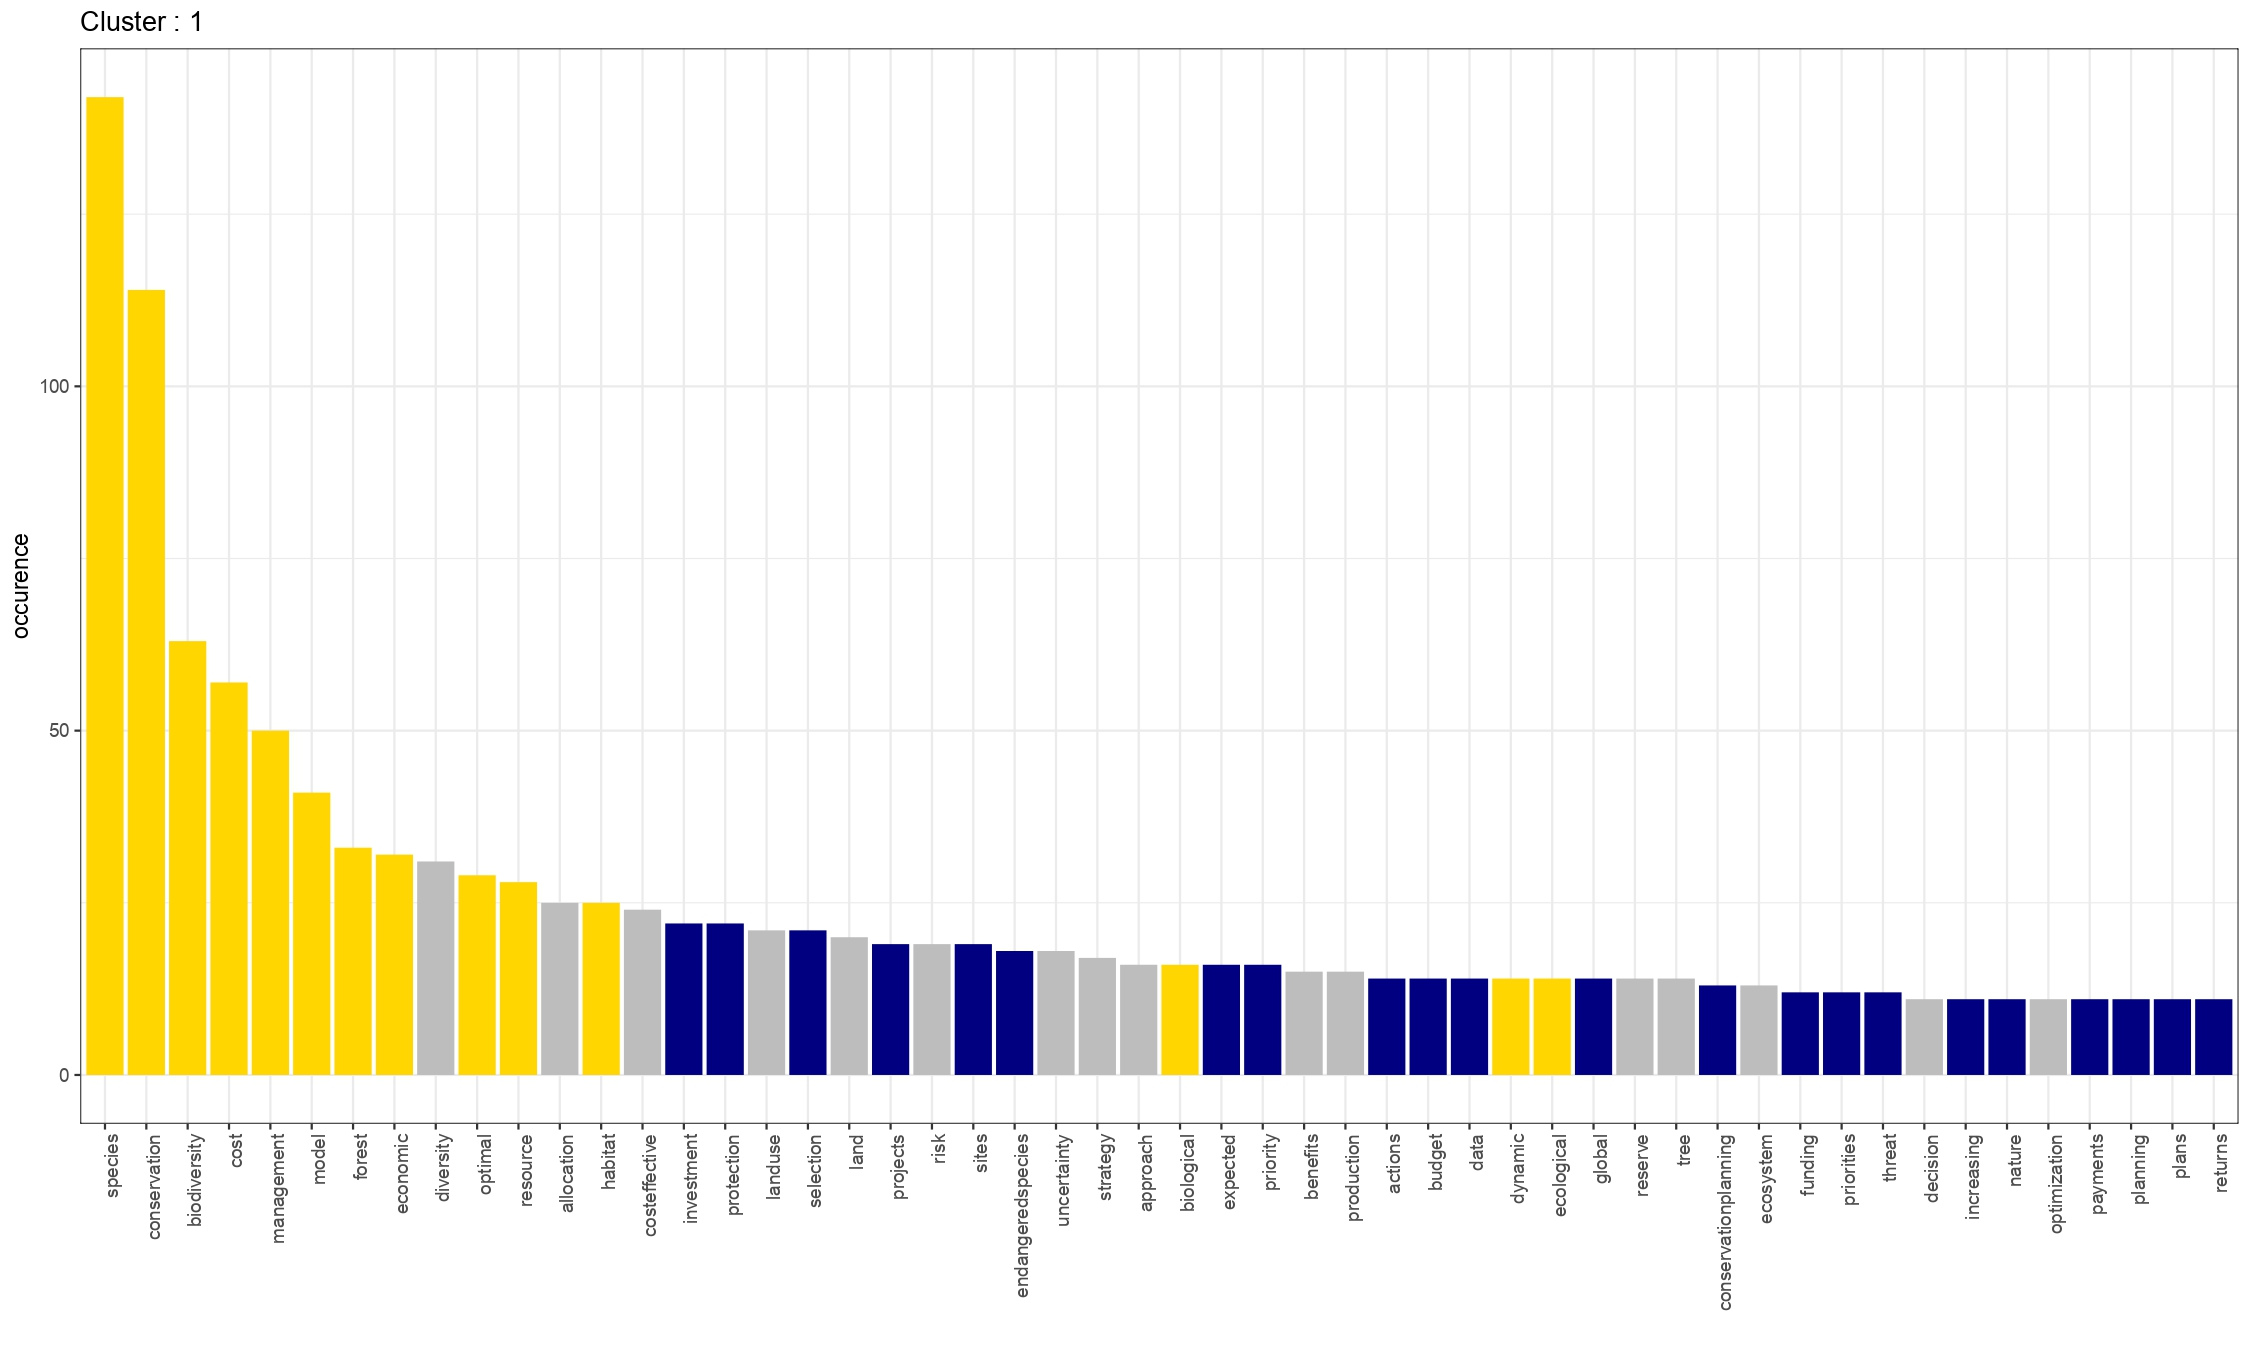
\includegraphics[width = .8\textwidth]{figures/review/occurence_kmodes_new_1_n50_common.png}\\
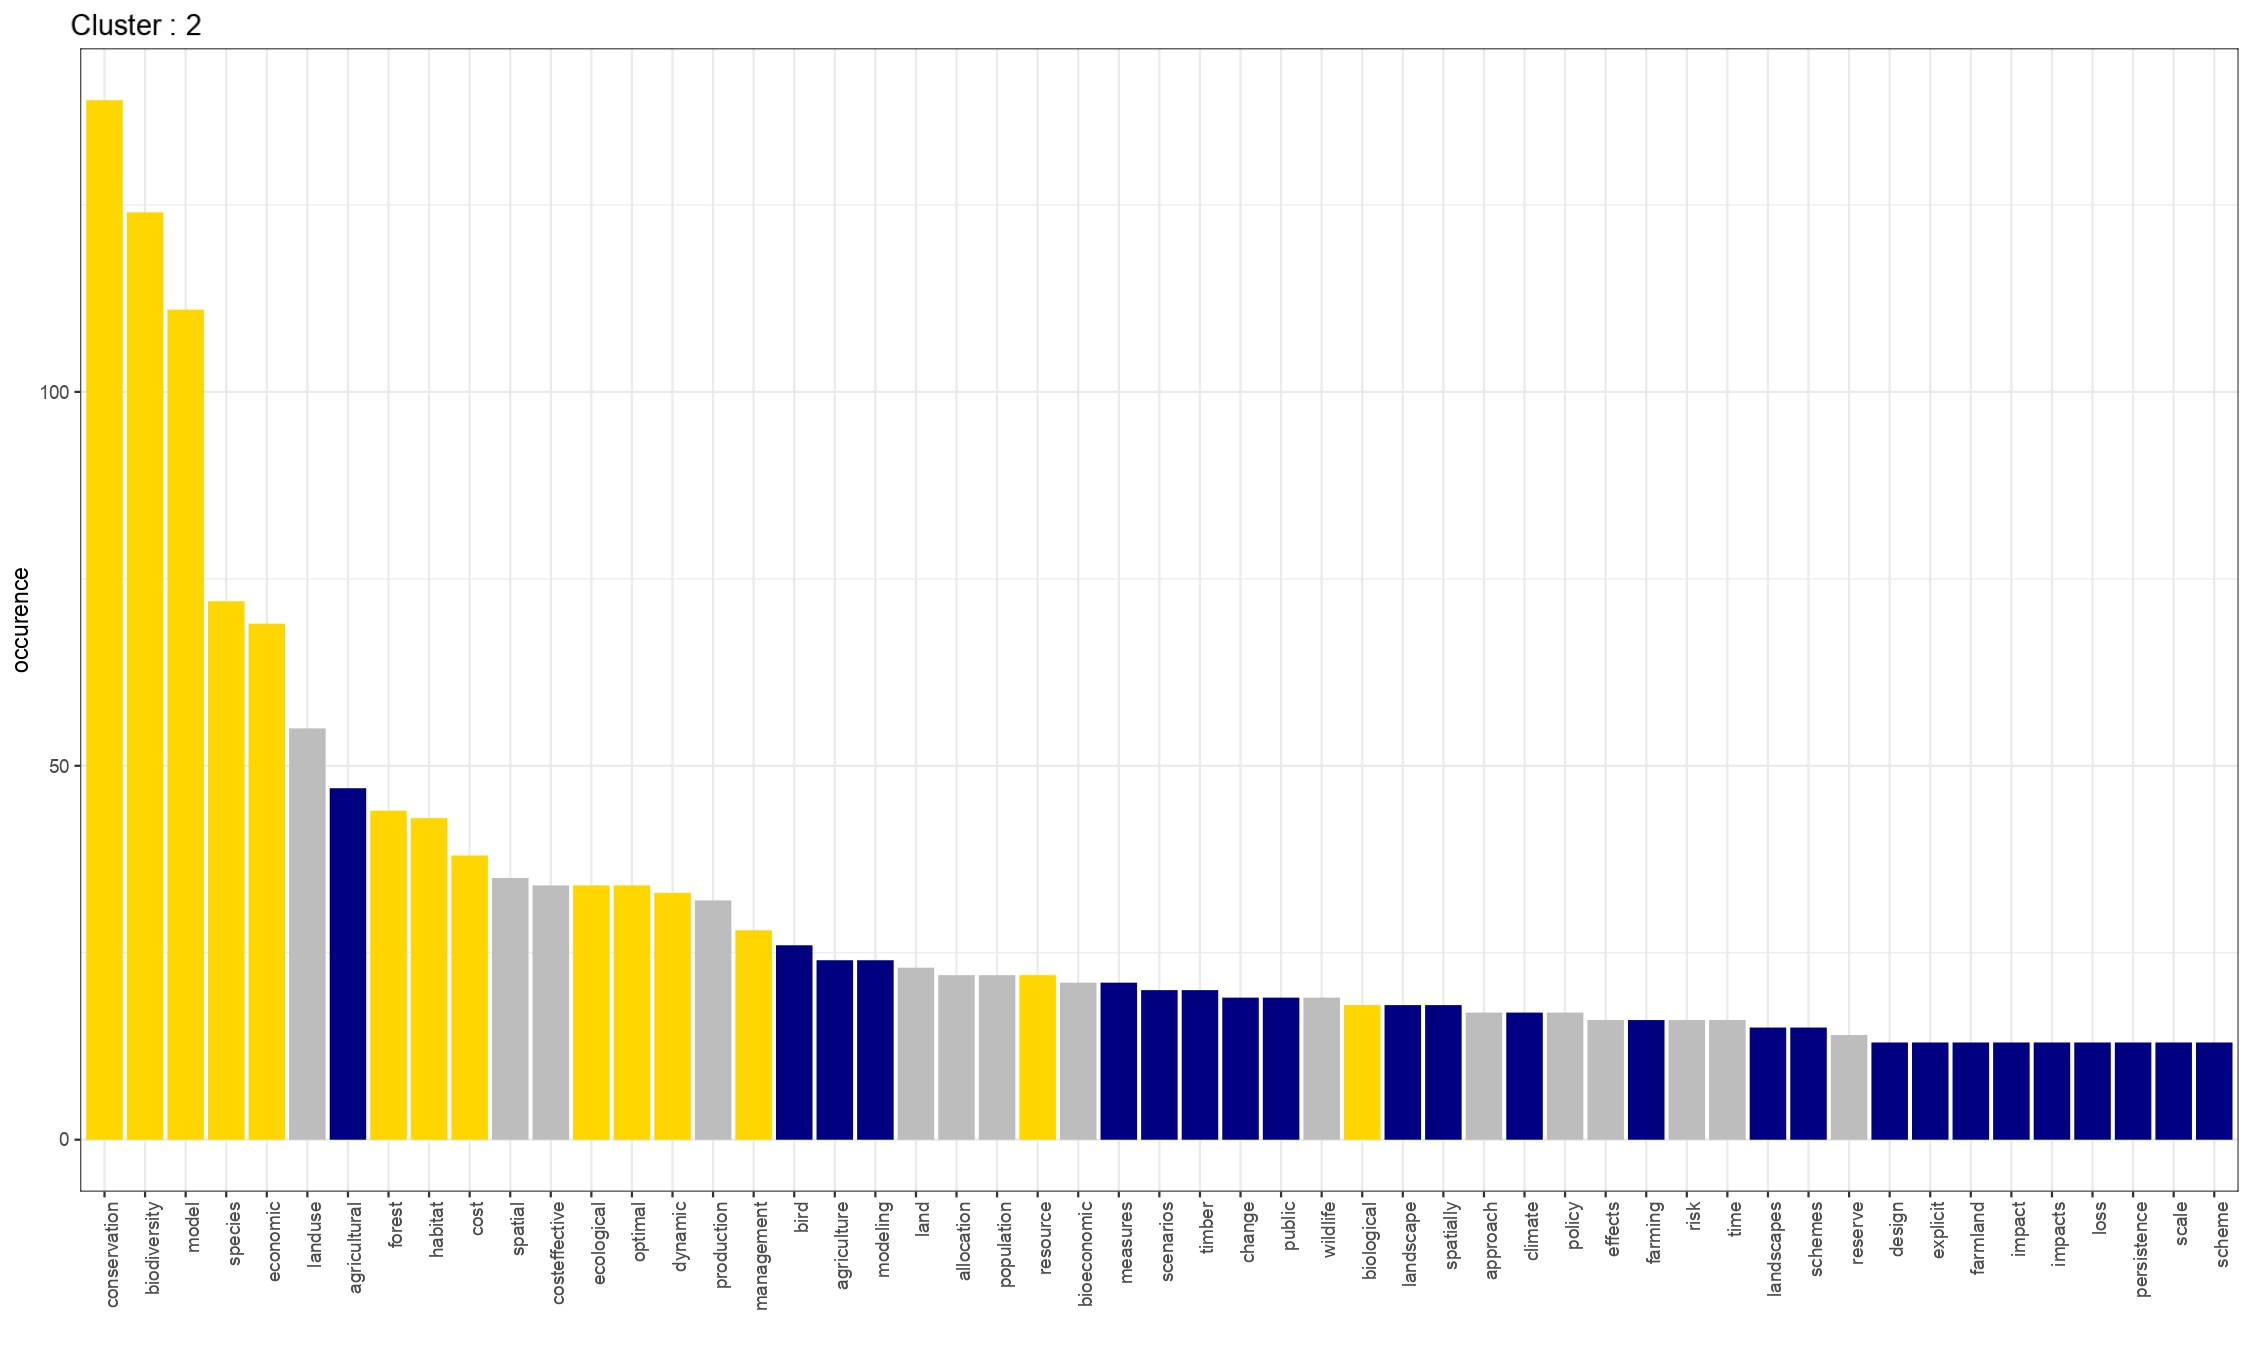
\includegraphics[width = .8\textwidth]{figures/review/occurence_kmodes_new_2_n50_common.png}
\caption{ Distribution profiles of the 50 words the more frequent for methodology-based groups 1 and 2}
\subcaption*{In yellow stand the words in common among the 4 profiles. On the opposite in blue stand the words specific to a profile}
\label{fig:words-profile-1}
\end{figure}

\begin{figure}[h]
\centering
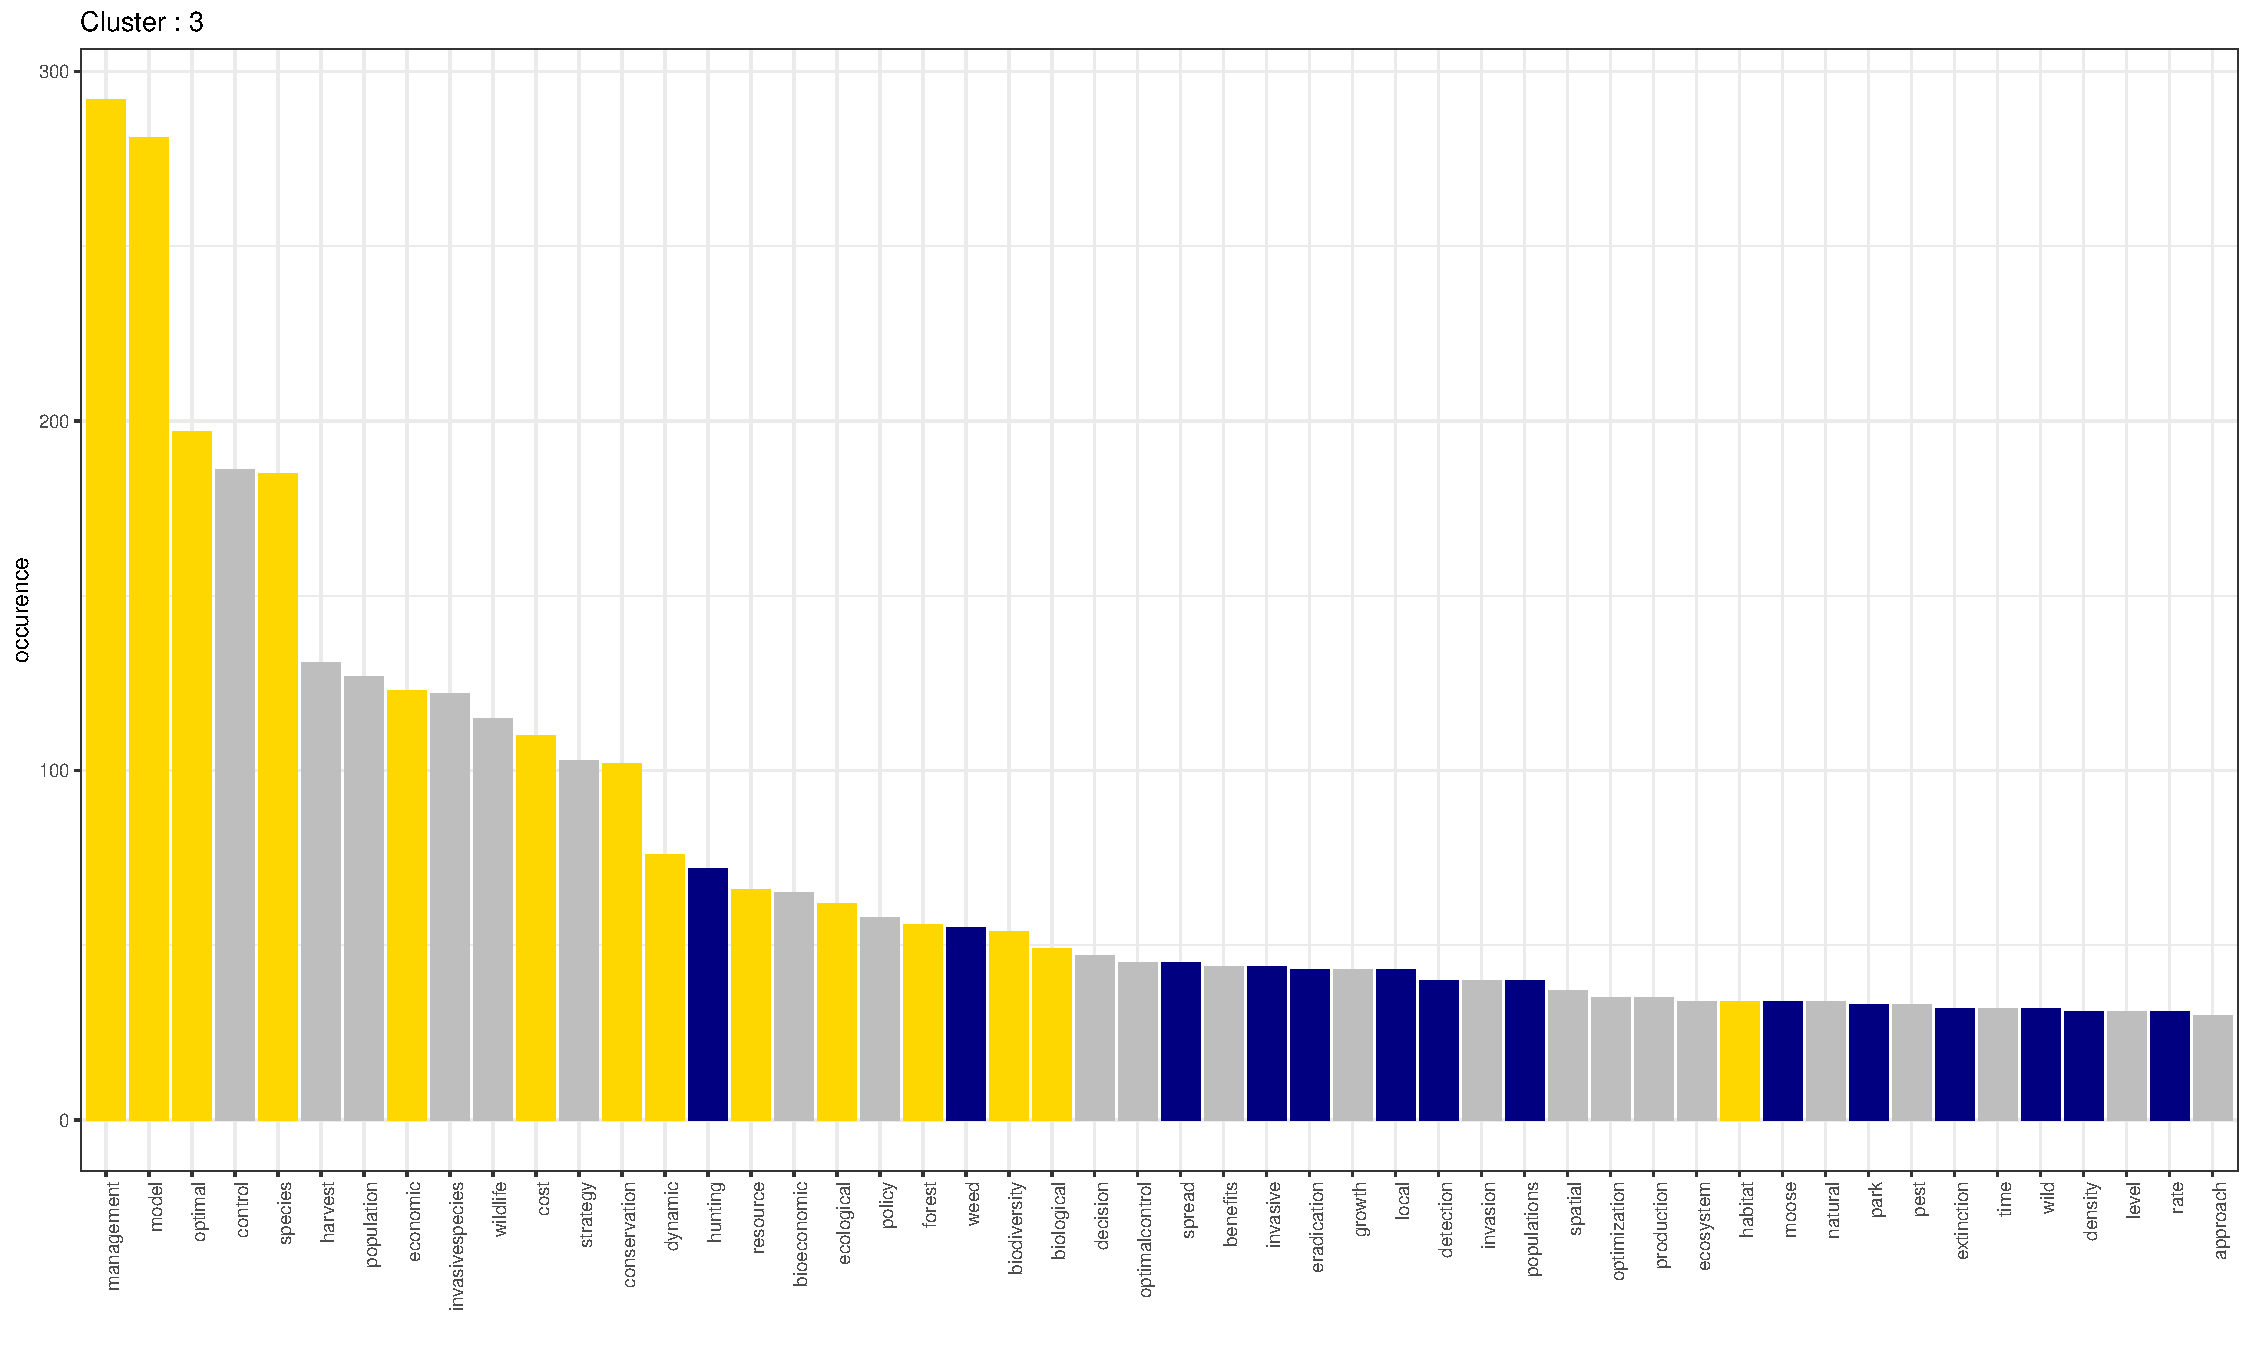
\includegraphics[width = .8\textwidth]{figures/review/occurence_kmodes_3_n50_common.pdf}\\
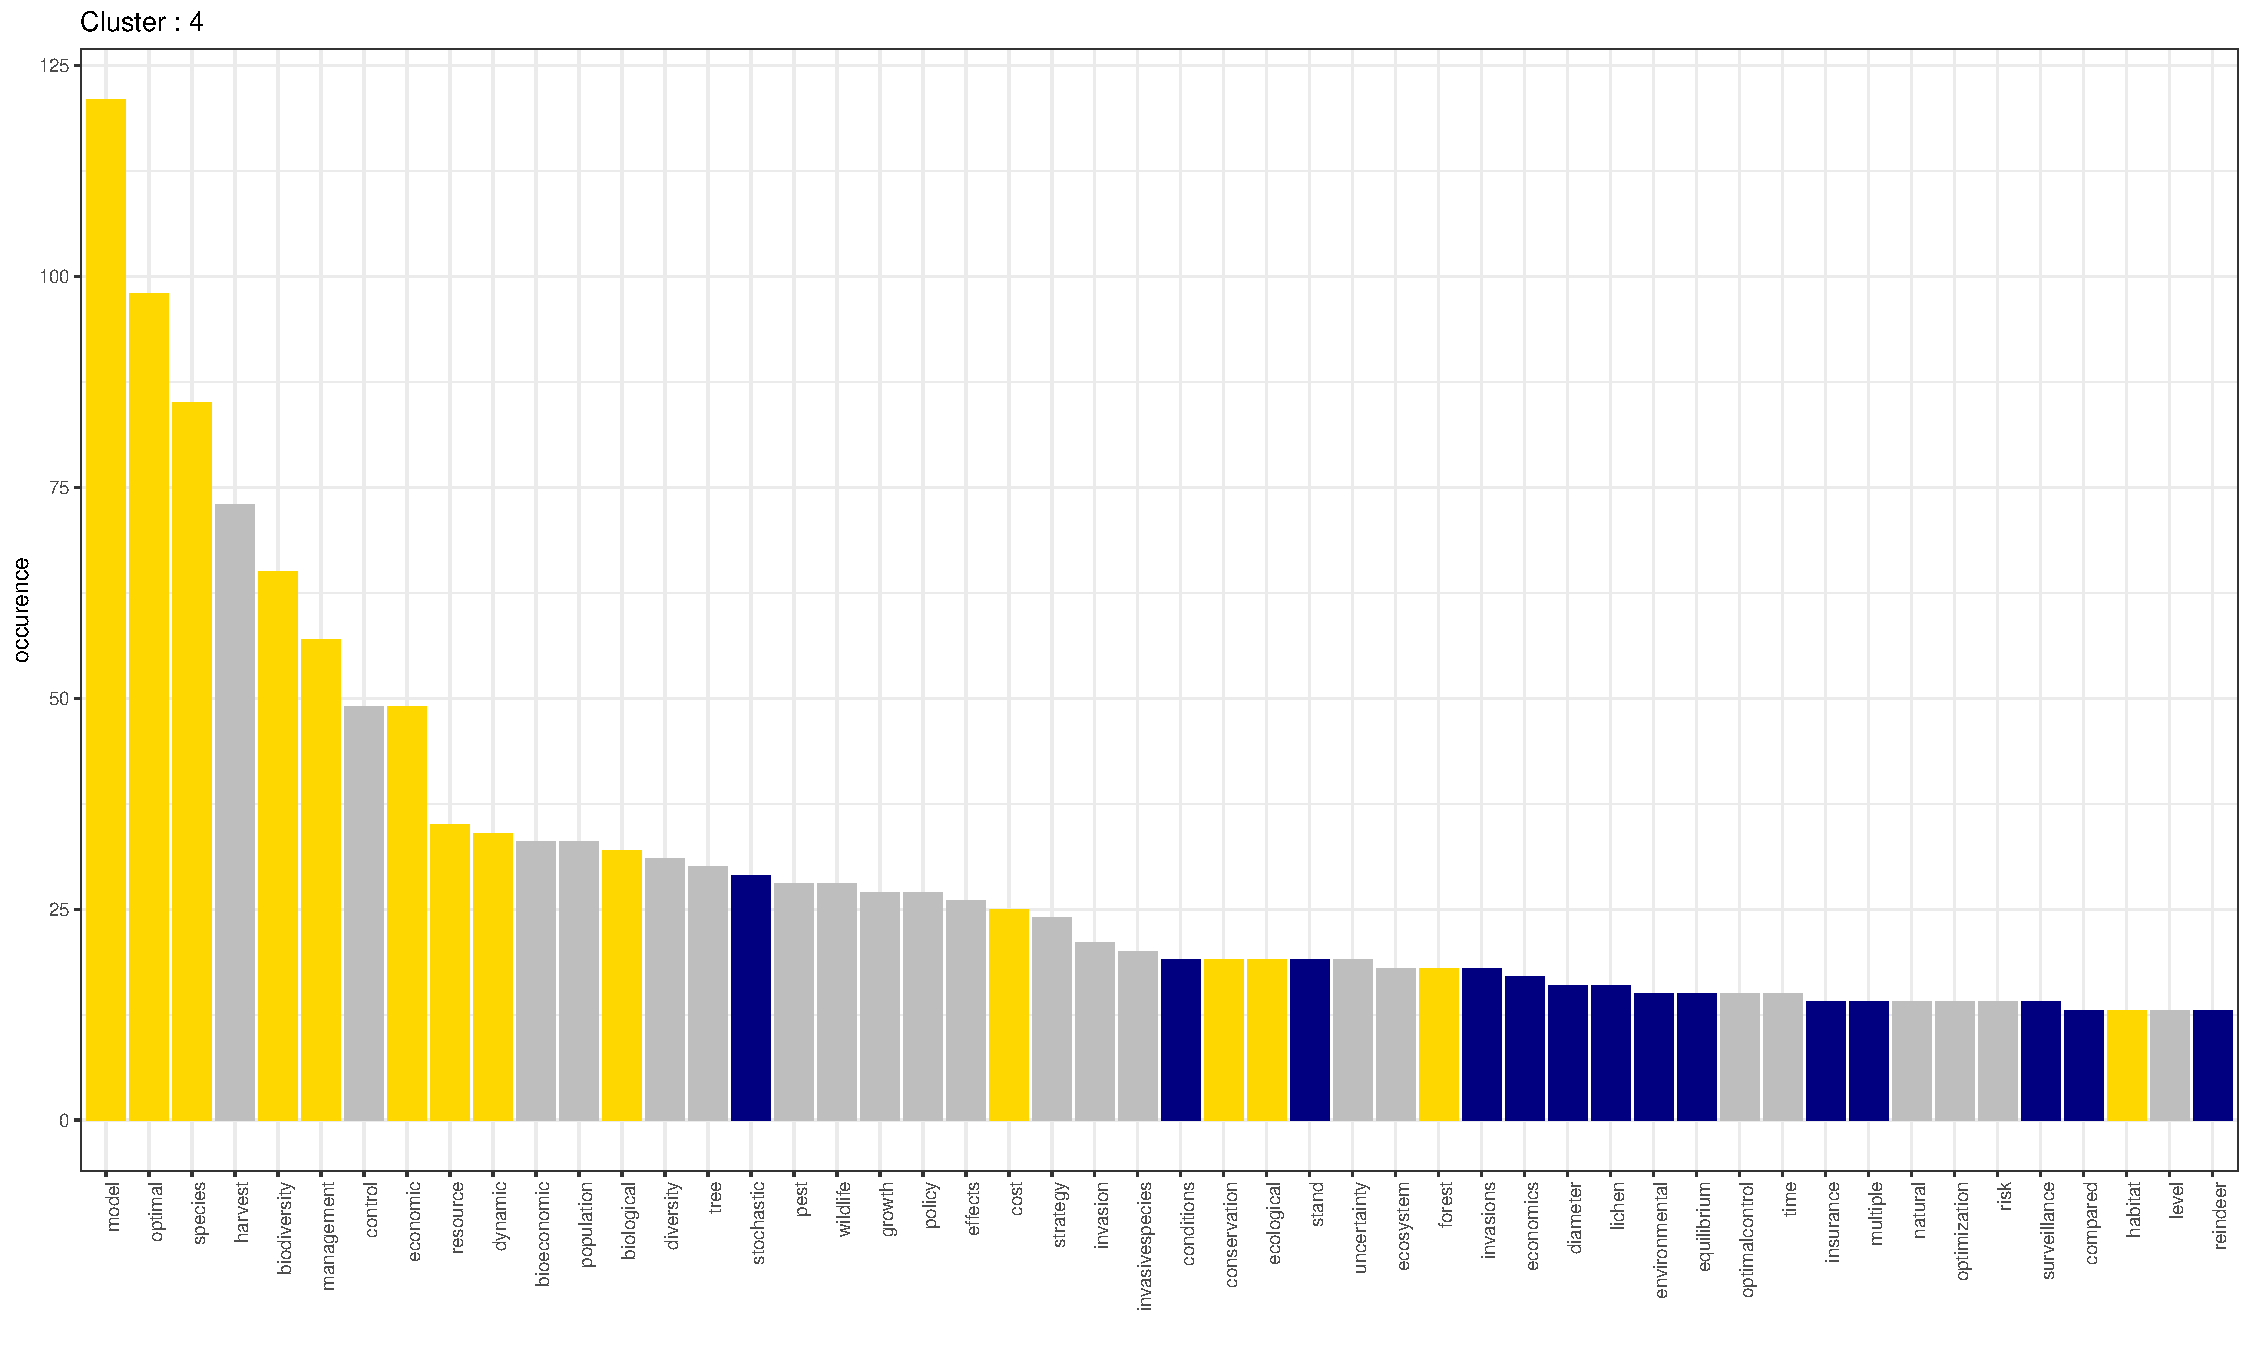
\includegraphics[width = .8\textwidth]{figures/review/occurence_kmodes_4_n50_common.pdf}\\
\caption{Distribution profiles of the 50 words the more frequent for methodology-based groups 3 and 4}
\subcaption*{In yellow stand the words in common among the 4 profiles. On the opposite in blue stand the words specific to a profile}
\label{fig:words-profile-2} 
\end{figure}

\begin{figure}[h]
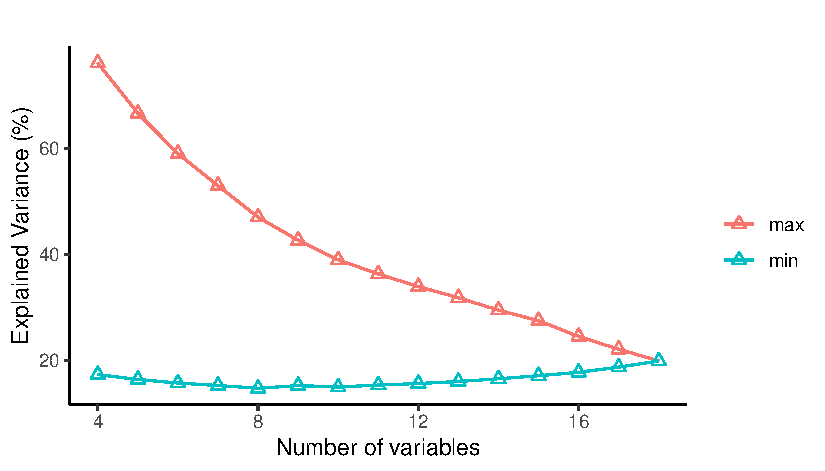
\includegraphics[width=.8\textwidth]{figures/review/variables_variance_enveloppe.pdf}
\caption{\label{fig:nb-crit-methodo} Explained variance function of the number of methodological criteria used in the MCA.}
\end{figure}

\begin{figure}[h]
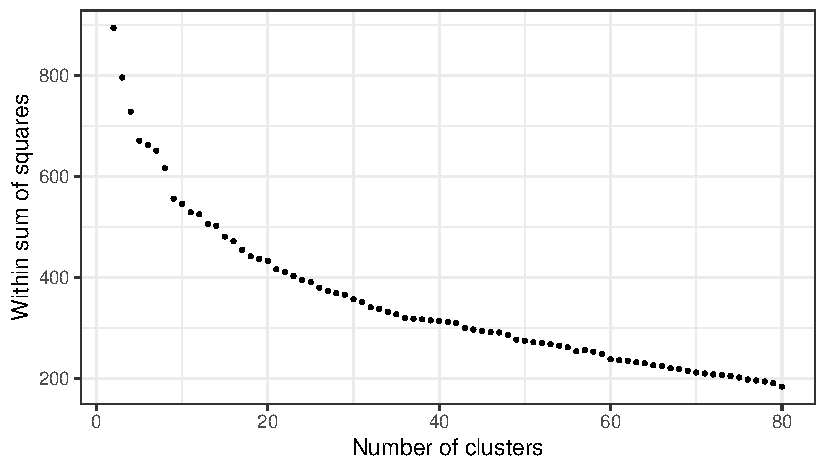
\includegraphics[width=.8\textwidth]{figures/review/kmodes_elbow.pdf}
\caption{\label{fig:cost-function} Cost function of the K-modes.}
\end{figure}

\begin{figure}[h]
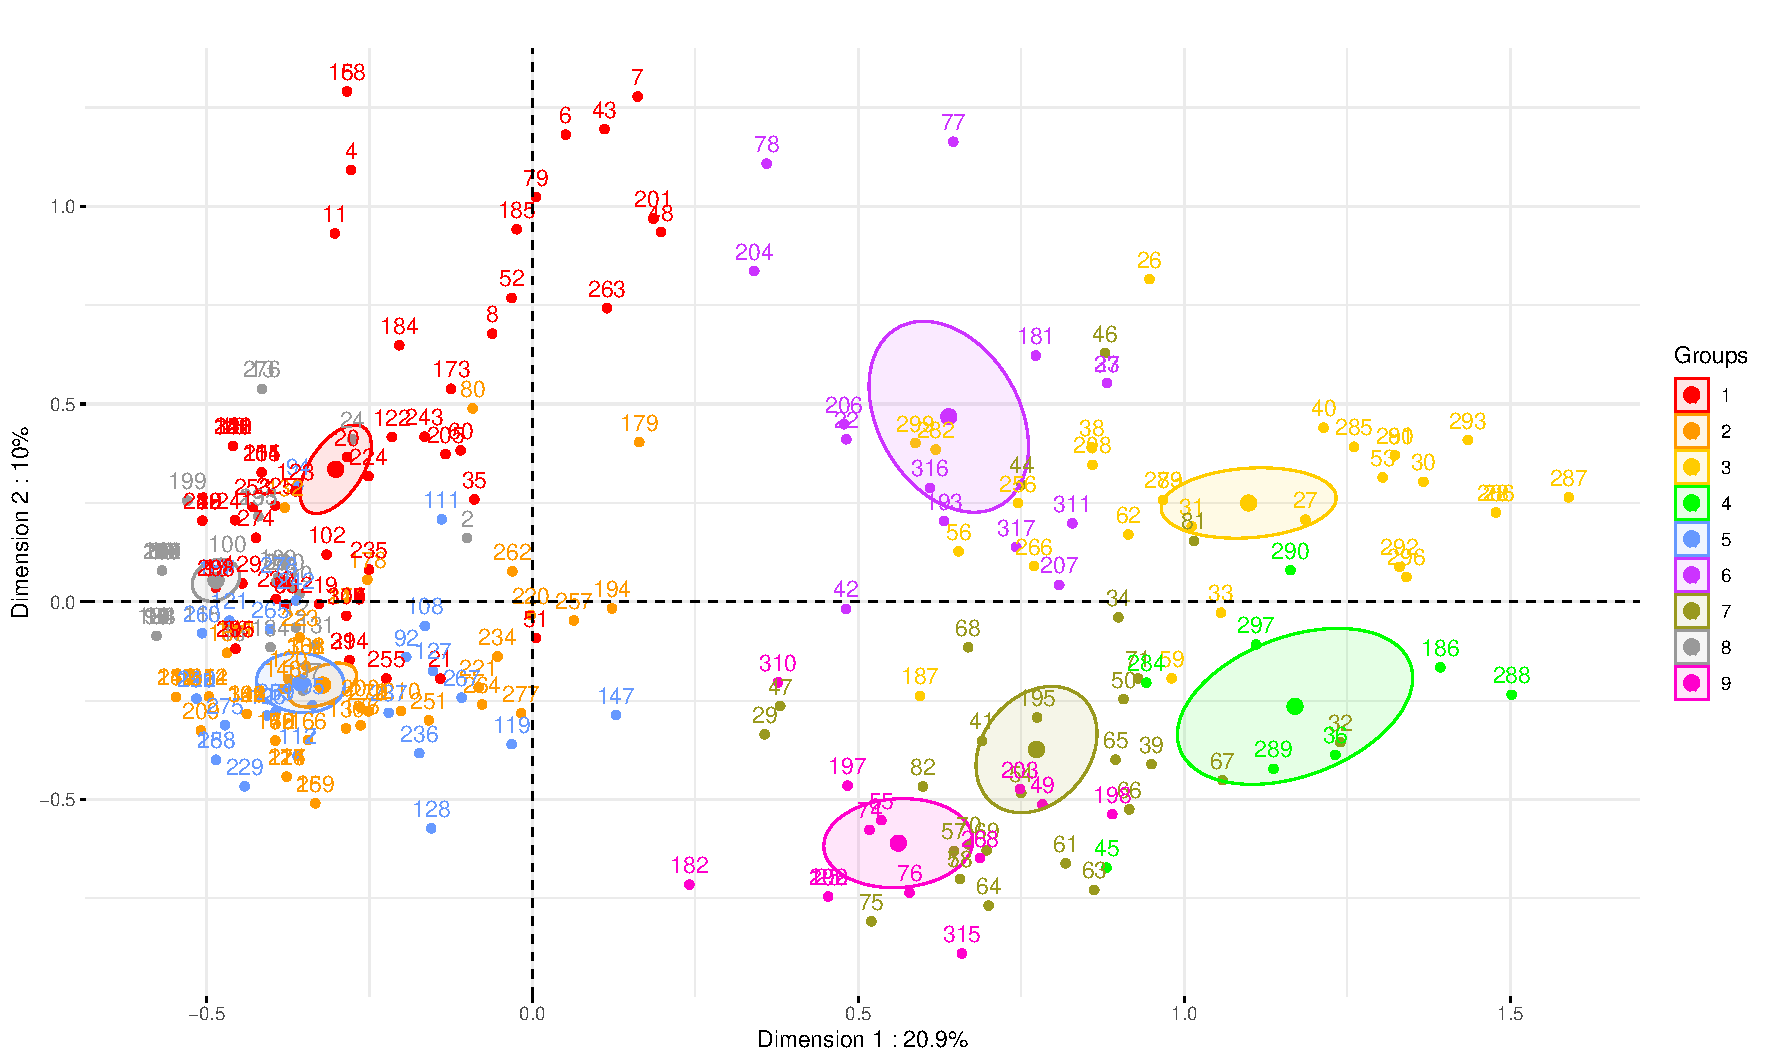
\includegraphics[width=.8\textwidth]{figures/review/mca_ind_automated_kmodes9.pdf}
\caption{\label{fig:MCA-9groups} Multiple Correspondence Analysis (MCA) running on 12 methodological criteria and 9 groups.}
\end{figure}
%	\end{appendices}		%
	\newpage
	\thispagestyle{empty}
%%%%%%%%%%%%%%%%%%%%%%%%%%%%%%%%%%%%%%%%%%%%%%%%%%%%%%%%%%%%%%%%%%%%
	%\part{Managing space and movement in terrestrial landscapes}
	% Maybe 1 page?
%%%%%%%%%%%%%%%%%%%%%%%%%%%%%%%%%%%%%%%%%%%%%%%%%%%%%%%%%%%%%%%%%%%%
	%
%%%%%%%%%%%%%%%%%%%%%%%%%%%%%%%%%%%%%%%%%%%%%%%%%%%%%%%%%%%%%%%%%%%%
%%%%%%%%%%%%%%%%%%% CHAPTER CONNECTIVITY %%%%%%%%%%%%%%%%%%%%%%%%%%%	
%%%%%%%%%%%%%%%%%%%%%%%%%%%%%%%%%%%%%%%%%%%%%%%%%%%%%%%%%%%%%%%%%%%%
	\renewcommand{\thesection}{\arabic{section}}
	\renewcommand{\thesubsection}{\arabic{subsection}}
	\setcounter{figure}{0}
	\setcounter{equation}{0}
	\counterwithout{figure}{section}
	\counterwithout{table}{section}
	\renewcommand{\thefigure}{2.\arabic{figure}}
	\renewcommand{\thetable}{2.\arabic{table}}
	\renewcommand{\theequation}{2.\arabic{equation}}
	\chapter{The wildfire-habitat connectivity dilemma: a graph theoretical approach to landscape management}

\begin{center}
\textbf{Abstract}\par
    \vspace*{.2cm}
    \noindent
    \begin{minipage}{0.9\textwidth}
	\singlespacing
\textbf{Background:} Fuel treatment operations help to mitigate the spread and severity of wildfires in numerous ecosystems. As they aim at fragmenting the fire landscape, they also fragment wildlife habitat. This poses a dilemma for land managers, in the form of a trade-off between lowering wildfire patch connectivity and maintaining wildlife habitat connectivity. Previous studies have investigated the spatial allocation of fuel treatments over time, mostly without specific care devoted to biodiversity, in a variety of case studies. However, they lack generality and an interpretative framework. We use dynamic programming and graph theory on every possible theoretical landscape configuration to gain a general understanding of the allocation of treatments over space and time and the corresponding landscape properties with various habitat connectivity targets. 
 
\textbf{Results:} Our results show that all initial landscapes converge to steady-state landscape cycles. Moreover, we show that there exist optimal trajectories that significantly reduce wildfire risk while safeguarding habitat connectivity. As the policy budget increases, more risk reduction is achieved, albeit with a decreasing marginal efficiency, and more steady-state cycles emerge. As habitat targets increase, increasing the budget is of no effect, and risk increases, while the number of steady-state cycles decreases. Landscapes are less risky, more fragmented, and diverse when the budget is large and biodiversity targets are low, while they are more compact and less diverse when the opposite is true. Treatment allocation follows graph centrality measures, and central cells are treated first. When the budget increases, fewer central cells (i.e. edge \textbf{patches}) are treated as well. When biodiversity targets increase, central cells are no longer treated as they decrease habitat connectivity. Treatment is reshuffled to the edges of the landscape.


 \textbf{Conclusion:} Computational experiments generalize existing results. Using graph theory, general insights can be gained, and help managers faced with multiple objectives in forested landscapes. From a policy perspective, in the face of climate change, increasing treatment budgets should be a priority to avoid increasing damages. A key guideline is treating a variety of seral stages to create landscape diversity, mitigate risk and guarantee the connectivity of wildlife habitat. 
\\
\textbf{Keywords : }Fuel treatment, connectivity, wildfire risk, wildlife habitat, spatial optimization, graph theory
\end{minipage}
\end{center}

\vfill
\newpage
\section*{To do}

\subsection*{Analysis}
\begin{itemize}
\item Run sample analysis for successive optimization
\item Compare outcomes
\begin{itemize}
\item Compare FPPs
\item Compare locations of treatments : centrality, degree etc
\item Compare landscapes characteristics
\end{itemize}
\item Need to think of the 5 period optimization v. the 3 age structure. 
\end{itemize}
\subsection*{Purpose of the paper}
\begin{itemize}
\item Launch all of the analysis : impossible for dynamic optimization
\item We do a subsample of 300 landscapes for real dynamic optimization: can generalize the findings 
\item We compare and find the general rules in a probabilistic sense
\item Then we find globally applicable rules of treatment allocation
\item Then we test them on large scale landscapes (100x100) and we test with different strategies: 
\begin{itemize}
\item Treat only old cells
\item Treat only young cells
\item Treat central cells
\item Treat a lot now, and less in the future (e.g. shift the budget towards today)
\end{itemize}
\end{itemize}

\subsection*{Rewriting}
\begin{itemize}
\item Justify why this is an economics problem
\begin{itemize}
\item We look at the social planner solution, and not the decentralized problem, because of the spatial, stochastic externality : space creates an interdependence and stochastic nature tends to cause underprotection.
\item Public ownership of land
\item Budget constraint
\item Scale 
\end{itemize}
\item Need to reinforce the widlfire risk/biodiversity relationship : 
\begin{itemize}
\item Redo literature review to link the two
\item Show clear examples with graphs
\end{itemize}
\item Need to reinforce our contribution in terms of what the problem is, and how our analysis is innovative : 
\begin{itemize}
\item Dynamic MILP : we do 5 periods : how do they relate to real life and how can we justify it? 
\item The former point implies the curse of dimensionality
\item In terms of graphs : we do not really do it in terms of coding, but we do it
\item NP hardness etc
\item Compare with existing literature, including the ones from the reviewers : network flow, or corridor : this is a single species view, or a hotspot to hotspot view, we do offer a view for multi level, multi functional biological diversity, not just the hotspots. THe question of the scale of movement of considered species is of course key. We adopt a broader view?
\item Need to write the model in a better way : fuck \textit{Fire Ecology}. 
\end{itemize}

\end{itemize}

\clearpage

\onehalfspacing
%%% Manuscript
\section{Introduction}
% Motivation : why should we care about wildfires? 
\hspace*{1.5em}Hazardous and intense wildfires destroy forest cover\footnote{From 2001 to 2023, forest loss attributed to wildfires amounted to 138 million hectares (roughly 33\% of the surface of the European Union) \citep{tyukavina_global_2022}}, threaten forest resilience and can cause ecosystem shifts, ranging from changes in forest structure to changes towards non-forest ecosystems \citep{coop_wildfire-driven_2020}. 
Additionally, intense wildfires cause human damages, in the form of direct asset losses: in 2018, wildfires in California have caused \$ 27 billion \citep{wang_economic_2021}. Indirect costs are also of concern, especially related to wildfire smoke : increases in PM 2.5 concentrations have important health impacts \citep{burke_wildfire_2023, heft-neal_behavior_2023}, smoke directly affects recreation values in the US, amounting to \$USD 2.3 billion in welfare losses \citep{Gellman}. Aside from directly measurable costs, wildfires also cause dramatic impacts on biodiversity across taxa \citep{Wintle2020}, through direct population losses and durable habitat disruption \citep{Ayars2023}.
%
\\
\hspace*{1.5em}In a business as usual scenario in terms of forest management, wildland-urban interface expansion and climate change, these direct and indirect costs and damages to both humans and non-humans are expected to increase drastically.
%
\\
Decades of wildfire suppression have created a ``wildfire deficit'', which increases the probability, extent and severity of wildfires in the western United States \citep{kreider_fire_2024}. European forests are not adapted to climate change induced wildfire risks \citep{Khabarov2014ForestFA}, in terms of species composition and use of fuel management operations. Mechanical thinning, prescribed burns, and sometimes, logging, have been leveraged to decrease the fuel load in risky areas and theoretically decrease the probability and severity of burns upon wildfire occurence\footnote{The efficiency of these measures depends on environmental and terrain variables. For example, prescribed burns are efficient every 1-4 years in reducing risk and severity only in the case of non-extreme weather conditions, and when the terrain ruggedness is limited \citep{bradstock_1998}}. In numerous regions, such as conifer forests in California \citep{Vaillant2009, Kalies2016, low_shaded_2023}, eucalypt forests in South Western Australia \citep{burrows2013, boer_long-term_2009, Florec2020}, southern Europe \citep{Fernandes2013}, evidence shows that fuel treatments, can mitigate wildfire intensity and spread. Land management agencies have historically implemented these policies in Australia \citep{burrows2013}, Europe, and the United States (and are projected to ramp up, for example under the Infrastructure Investment and Jobs Act of 2021 in the US). While potentially useful, the use of these treatments is still hindered by numerous obstacles \citep{miller_barriers_2020} and remains insufficient \textbf{ref}\footnote{However, recent bills have been passed in the US (Infrastructure Investment and Jobs Act of 2021) and California to ramp up the use of prescribed burns - such as \href{https://wildfiretaskforce.org/about/expenditure-plan/}{the bugdget act of 2022}, committing \$2.8 billion to the Governor’s Wildfire and Forest Resilience Action Plan - and limiting liabilities in the case of wildfire escape (see \href{https://openstates.org/ca/bills/20212022/SB332/}{California Senate Bill SB-332}) on private land.}. 
Additionally, the extension of wildland-urban interfaces (WUI) increases the extent of potential damages as well as ignition probabilities \citep{radeloff_rapid_2018}.
\\
As global warming affects water supply and fuel moisture \citep{jolly_climate-induced_2015, Abatzoglou, ruffault_extreme_2018}, it is projected to increase the frequency, severity, and magnitude of wildfires \citep{Dupuy2019ClimateCI, wasserman_climate_2023}. Recent wildfire events in California (since 2018), in Australia (2019-2020), and in Europe (France, Portugal, Greece in 2022) have epitomized these trends. 
%
Moreover, wildfires and climate change are endogeneously linked in a positive feedback loop : large wildfires are of importance in the face of climate change; as they release large amounts of greenhouse gases ($1.7GtC$ per year on average between 2003 and 2022) and reduce the extent of terrestrial carbon sinks \citep{zheng_record-high_2023, friedlingstein_2023}. \\
\hspace*{1.5em}In the face of a growing threat to human assets and biological diversity, increasing the efficiency of fuel treatments to manage multiple objectives is paramount. A decision framework that accounts for wildfire processes and biological diversity drivers is paramount to deliver policy recommendations that simultaneously achieve widlfire damage reduction and protect biological diversity \citep{driscoll_resolving_2010}. Among the decision levers, the extent and location of treatments are key variables. 
%
\\
By changing the structure of the landscape, fuel management operations may reduce the risk and associated damages of wildfires. Treatments achieve larger risk reduction when located close to the values at risk instead of being dispersed across the landscape \citep{ager_modeling_2007, Williams2017,Florec2020}. However, they also affect the structure of biodiversity habitat, notably, its structural connectivity \citep{Taylor93}. Maintaining habitat connectivity, through wildlife corridors, landscape links, and ecoducts \citep{Turner2005, Turner2011}, is instrumental in mitigating the biodiversity crisis. Species richness and diversity are intimately linked to landscape connectivity \citep{Olds2012, tian_assessing_2017, velazquez_structural_2019} and are necessary to maintain ecosystems in the future. Fragmentation, conditional on habitat surface being constant, may enhance biodiversity \citep{tischendorf_usage_2000, hu_effects_2012, may_geometry_2019}. However, it is often accompanied with habitat loss, detrimental to biodiversity \citep{fahrig_effects_2003}. The use of fuel management operations alters the structure of the landscape e.g. both habitat and matrix\footnote{e.g. land use or cover, or environmental conditions that differ from eitehr species' habitat or reference natural conditions \citep{fletcher_prominent_2024}}, in terms of temporal and spatial variation in landscape configuration and composition. As habitat is altered, so is the surrounding matrix, which can impede species movement \citep{eycott_meta-analysis_2012, kuefler_conflicting_2010} and alter evolution and selective regimes \citep{cheptou_adaptation_2017}.\\
The impact of fuel treatments on biodiversity remains a debated topic. 
Evidence suggests that maintaining a variety of vegetation types and ages on a patchy landscape maintains a 'fire mosaic' \citep{Sitters2015} (e.g. landscape level variations in habitat types that provide habitat to an ecological community) or that fuel treatment can be beneficial to wildlife \citep{saab_short-term_2022, loeb_bats_2021} and even restore local populations \citep{Templeton2011}. On the other hand, treating at too high a frequency may be detrimental to biodiversity \citep{bradshaw2018}, as vegetation with extensive juvenile period may disappear, and fauna that rely on them as well\footnote{For example, in Australia, species such as \textit{Banksia baueri}, \textit{B. nutans} and B. \textit{baxteri} would disappear, threatening tammar wallabies, quokas and honey possums \citep{bradshaw2018}}, or high frequency treatment favors the invasion of fire tolerant, fire-enhanced weed species \citep{vanWilgen_fire_2013}. 
%
\\
Hence, fragmenting the wildfire risk poses significant threats to biodiversity in forest landscapes. Nonetheless, there may exist a range of spatial allocation patterns that take into account the location of protected species and can reduce threats to both assets and biodiversity \citep{ager_modeling_2007, king_relative_2008, rachmawati_fuel_2018}. 
\\
\hspace*{1.5em}Eventually, wildfire risk and potential damages pose a significant challenge in terms of policy-making. As wildfire risks and potential damages are spatially heterogeneous, and as wildfires spread, they create a large spatial externality. Indeed, individual risk reduction is hampered by the influence of neighbors on individual risk, which results in the under provision of risk reduction \citep{SHAFRAN2008488, costello_private_2007}. Additionally, in a risky (e.g. stochastic) context, risk aversion may bolster this phenomenon when financial insurance is limited \citep{ehrlich_market_1972}\footnote{This is particularly the case in California, where repeated fire episodes have pushed insurers to \href{https://calmatters.org/economy/2024/05/california-insurance-mitigation/}{spike contract premiums}, or \href{https://www.nbclosangeles.com/news/california-wildfires/state-farm-california-los-angeles-homeowners-insurance-policy/3383583/}{to not renew contracts}- non renewal rates went from 11\% in 2018 to 13\% in 2021}. Finally, the magnitude of potential damages \citep{costello_private_2017} as well as the large information requirements for efficient fuel treatment planning warrant a collective approach.
\\
\hspace*{1.5em}In this context, we study the spatial patterns of treatment allocation that diminish potential damages from wildfires in where fire spread is governed by patch connectivity, while safeguarding biodiversity habitat connectivity, from a central decision maker perspective.  
\\
\hspace*{1.5em}A substantial literature has applied optimization techniques to tackle the spatial allocation of fuel treatments. Analytical \citep{finney_design_2001}, simulation-based \citep{finney_computational_2007, rytwinski_simulation-optimization_2010} or mixed-integer programming techniques \citep{wei_optimization_2008} have solved the allocation of treatments in a static framework. Given the dynamic nature of fuel growth, studies based on mixed-integer dynamic programming \citep{wei_optimization_2008, minas_spatial_2014, rachmawati_model_2015, rachmawati_optimisation_2016} have studied the temporal and spatial allocation of fuel treatments on real and simulated landscapes. While they solve the spatial treatment allocation problem in forests, these articles fail to acknowledge the multiple uses and objectives land planners have to consider, such as habitat conservation. Several articles have devoted their attention to the spatial allocation of treatments while conserving habitat, and investigated the trade-offs between risk reduction and biodiversity conservation, using spatial heuristics \citep{calkin_modeling_2005, lehmkuhl_seeing_2007} and linear programming \citep{Williams2017, rachmawati_fuel_2018}.\\
Most of the existing literature focuses on case studies and lacks a general interpretative framework to generalize its results. Graph theory offers a toolbox suited to analyze the properties of connected cells or patches of land with varying characteristics, and has extensively been applied in landscape ecology \citep{urban_landscape_2001, minor_graph-theory_2008, rayfield_multipurpose_2016}. \cite{conrad_wildlife_2012} and \cite{jafari_new_2013} use a specific graph theory algorithm - a network-flow model - to find the optimal subgraph of corridors connecting habitat areas. Their approach optimally connects patches of habitat spread across the landscape for a given species, in a reserve-network design problem fashion. Our approach adopts a more holistic perspective, as it emphasises the degree of connectedness between habitat cells, thus allowing for a multi-species and multi-scale perspective, instead of a corridor for a single species.  
\\
Recent research focusing on the allocation of fuel treatments has leveraged tools from graph theory \citep{matsypura_wildfire_2018, pais_downstream_2021}. Reconciling habitat and wildfire risk mitigation using graph theory is a recent research endeavor \citep{rachmawati_fuel_2018, yemshanov_exploring_2022} and has focused on specific case studies. 
\\\\
\hspace*{1.5em} In this article, we focus on the dynamic and spatial dimensions of the problem (thus abstracting from the stochastic components) and leverage graph theory to study the general patterns of treatment allocation emerging from a multi-objective, dynamic, and integer landscape management problem, governed by connectivity. \\
To do so, we first compare the optimal allocation of treatments using repeated static optimization and heuristic dynamic programming on a 5 period horizon on representative subsamples of small scale landscapes with an exhaustive range of habitat connectivity constraint. We show that for realistic biodiversity habitat constraint levels, the constraint imposed on the evolution of the forest results in similar structures for repeated myopic and dynamic optimization. Therefore, we analyse the treatment allocation and landscape structures emerging in the long run using repeated myopic optimization for all the possible initial landscape configurations, in a graph theoretical framework. We explicit the trade-off between risk reduction and biodiversity habitat, in the form of a production possibility frontier (PPF). We characterize the landscapes using a range of ecological indicators and find general mechanisms and guiding principles applicable to a broad class of settings, to guide decision-makers and foster new efficient multi-objective graph theory algorithms. Finally, we test our predictions from a small scale landscape to simulated realistic large scale landscapes (10,000 cells)  with varying composition and spatial autocorrelation, and compare them with different intuitive policy recommendations. 
\\
Our contributions are several. First, we provide a spatial framework to understand the trade-offs between wildfire risk reduction and biodiversity conservation. Second, we leverage the constraints imposed on a dynamic spatial system to show that repeated optimization performs relatively well compared to dynamic programming. Third, using graph theory, we derive general principles regarding the spatial characteristics of landscapes and treatments from an exhaustive set of theoretical landscapes to guide policymakers as well as future research in heuristics to reconcile conflicting land-based phenomenons.
%Eventually, we characterize the risk and biodiversity profiles consistent with a changing climate, where windows of opportunity are shorter and costs of treatment larger, and the associated spatialized treatments. 
\\
This article is structured as follows : section \ref{section:methods} explains our methods, section \ref{sec:results} explains our results, and section \ref{section:discussion} discusses our results and concludes. 

\section{Methods}
\label{section:methods}
\subsection{Model description}

%\subsection{Context}
We consider landscapes represented by a regular grid of $n\times n$ standardized area cells in period $t$ by $\mathbf{A}_t$ with a forest seral stage succession module. 
%We denote by $\mathbf{A}_t$ the matrix of standardized area cells in the theoretical landscape of dimension $n\times n$ (hereafter referred to as being of size$=n$) in period $t$. 
Each cell $a_{ijt} \in \mathbf{A}_t$ with $\{i,j\} \in \{1, ...,n\}^2$, at time $t$ is characterized by a successional stage: \textit{juvenile}, \textit{adolescent}, or \textit{mature}, which translates into 3 numerical age classes ranging from 0 to 2. 
Each transitionary seral stage has the same duration\footnote{For example, in Australia, \cite{mccoll_gausden_pathways_2019} use quasi evenly spaced age classes for heathland, tall-mixed, foothills, forby and wet vegetation types (see table 1); on the other hand, in coniferous forests in Western US (Washington and Oregon),\cite{thomas_wildlife_1979} developed a successional stage description for wildlife habitat management, \href{https://www.fs.usda.gov/Internet/FSE_DOCUMENTS/stelprdb5413728.pdf}{still used by the USDA}. 40 year transitional classes can be made grouping \textit{grass-forb, shrub-seedling and pole-sapling} together and \textit{young}. \textit{Maturity} is reached at 80 until 159 years old, where it mutates into \textit{old-growth}}, hence at each time step, it changes stage until it is in the \textit{mature} stage, where it remains (eq \ref{eq:fuel_dyn})

We use a stylized representation of the link between vegetation age, habitat, and wildfire risk (figure \ref{fig:illustration}). \\
First, we assume a cell offers suitable wildlife habitat once it is \textit{adolescent} (eq. \ref{eq:mature}). Second, a cell can turn at critical risk of wildfire during a normal hot season when its successional stage is \textit{mature} (eq. \ref{eq:high_fuel}). We assume an Olsen-type model of flammability, where age class is the main predictor of flammability \citep{Olson1963,mccarthy_theoretical_2001,mccoll_gausden_pathways_2019}. A cell remains at high risk as long as it is in the \textit{mature} age class. \\
Finally, we consider fuel treatment to be a binary decision e.g. treatment is absent or present and there is no extensive margin, hence a treatment binary variable $x_{ijt}\in\{0,1\}$ represents the treatment status in cell $a_{ij}$ a time $t$. The decision maker first observes the transition to the next successional stage, then decides upon treatment.
Treatment can happen at any successional stage : whether at an \textit{adolescent} stage, in anticipation of a cell becoming \textit{mature} and turning at \textit{high risk} in the next period, or as an immediate strategy upon becoming \textit{mature} and thus, \textit{high risk}.
Upon treatment, a cell successional stage is reset to \textit{juvenile} (eq. \ref{eq:fuel_dyn}). Figure \ref{fig:illustration} illustrates the dynamics of the model.

Given a patch $a_{ijt}$ and treatment status $x_{ijt}$ in period $t$, equation \ref{eq:fuel_dyn} summarises the successional dynamics, and equations \ref{eq:high_connectivity},\ref{eq:high_fuel} summarize the link between successional stage, habitat, and high risk: $\forall t, \forall \{i,j\} \in \{1,..., n\}^2$

%\begin{minipage}{0.45\textwidth}
   \begin{align}
a_{ijt+1} &= \max \large((a_{ijt} + 1)(1-x_{ijt}); 2 \large)
\label{eq:fuel_dyn}\\
Habitat\left(a_{ijt}\right) &= \begin{cases}
        1 &\text{ if } a_{ijt} \geq 1\\
        0 &\text{ otherwise }
    \end{cases}
\label{eq:mature}\\
Risk\left(a_{ijt}\right) &= \begin{cases}
1 &\text{ if }a_{ijt}\geq 2\\
0 &\text{ otherwise}
    \end{cases}
\label{eq:high_fuel}
\end{align}
%\end{minipage}%
\hfill
\begin{figure}
    \centering
    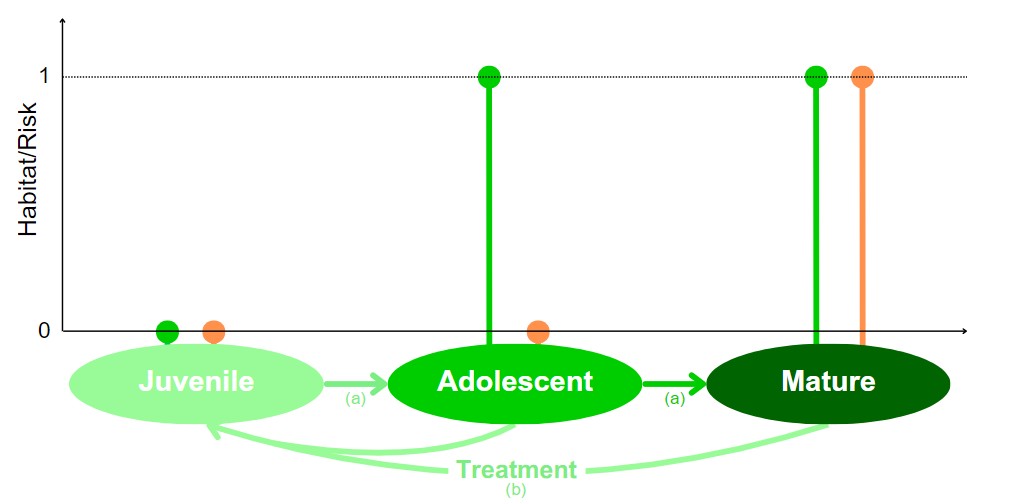
\includegraphics[width = .6\textwidth]{figures/wildland/Juvenile.png}
    \caption{Illustration of the successional stages and the link between successional stage, habitat and wildfire risk using a discretized Olson-type relationship}
    \subcaption*{At the bottom, the dynamics of the model are illustrated. First, successional stages transition (step (a)), then treatment is applied (step (b)). At the top, the link between successional stage, habitat and high risk. In green, a \textit{habitat} variables turns to $1$ when a cell is \textit{adolescent}, and in orange, a \textit{high risk} dummy turns to $1$ when a cell turns \textit{mature}} 
    \label{fig:illustration}
\end{figure}
%\end{minipage}%


%\subsection{Theoretical model}

We use a network structure to apprehend the landscapes. From the matrix $\mathbf{A}_t$, we form two graphs:  $\mathcal{B}_t = (V_{\mathcal{B}_t}, E_{\mathcal{B}_t})$, the graph of suitable habitat cells and $\mathcal{F}_t = (V_{\mathcal{F}_t}, E_{\mathcal{F}_t})$, the graph of high risk cells. First, the vertices of each graphs are the suitable habitat cells e.g $
V_{\mathcal{B}_t} = \{(i,j)$ such that $Habitat(a_{ijt})=1\}$ and the high risk cells, respectively e.g. $V_{\mathcal{F}_t} = \{(i,j)$ such that $Risk(a_{ijt})=1\}$.\\
Second, vertices are connected if they are within a Moore (or 8-cell) neighborhood of each other and share the same status. Therefore, notice that $\mathcal{F}_t\subset \mathcal{B}_t$. Figure \ref{fig:graph_overlap} illustrate the mechanism from the landscape in matrix form $\mathbf{A}_t$ with age classes ranging from 0 to 2, to graphs $\mathcal{B}_t$ and $\mathcal{F}_t$.

We use this 8-cell neighborhood for evaluating biodiversity habitat and wildfire risk within a common a spatial framework, using the same adjacency properties. 
Regarding biodiversity, we focus on general characteristics related to landscape structural connectivity rather than functional connectivity, as we are agnostic about effective species \citep{Fahrig2011}. We assume that species are able to disperse from one patch to another, and that habitat quality is uniformly distributed conditional on habitat being available.\\
We consider the wildfire risk through the lens of potential spread, influenced by fuel, wind direction and terrain. We abstract from wind patterns and terrain, to focus on fuel connectivity\footnote{Note that our framwork is amenable to prevailing wind patterns and terrain ruggedness, as the graph adjacency matrix can change from a Moore adjacency to any pattern influenced by environmental features}. Consistent with the literature (see \cite{Peterson_2009}, \cite{pais_cell2fire_2021, gonzalez-olabarria_fire_2023}), a wildfire can spread in any direction, conditional on neighbor cells with high risk. 

\begin{figure}
    \centering
    %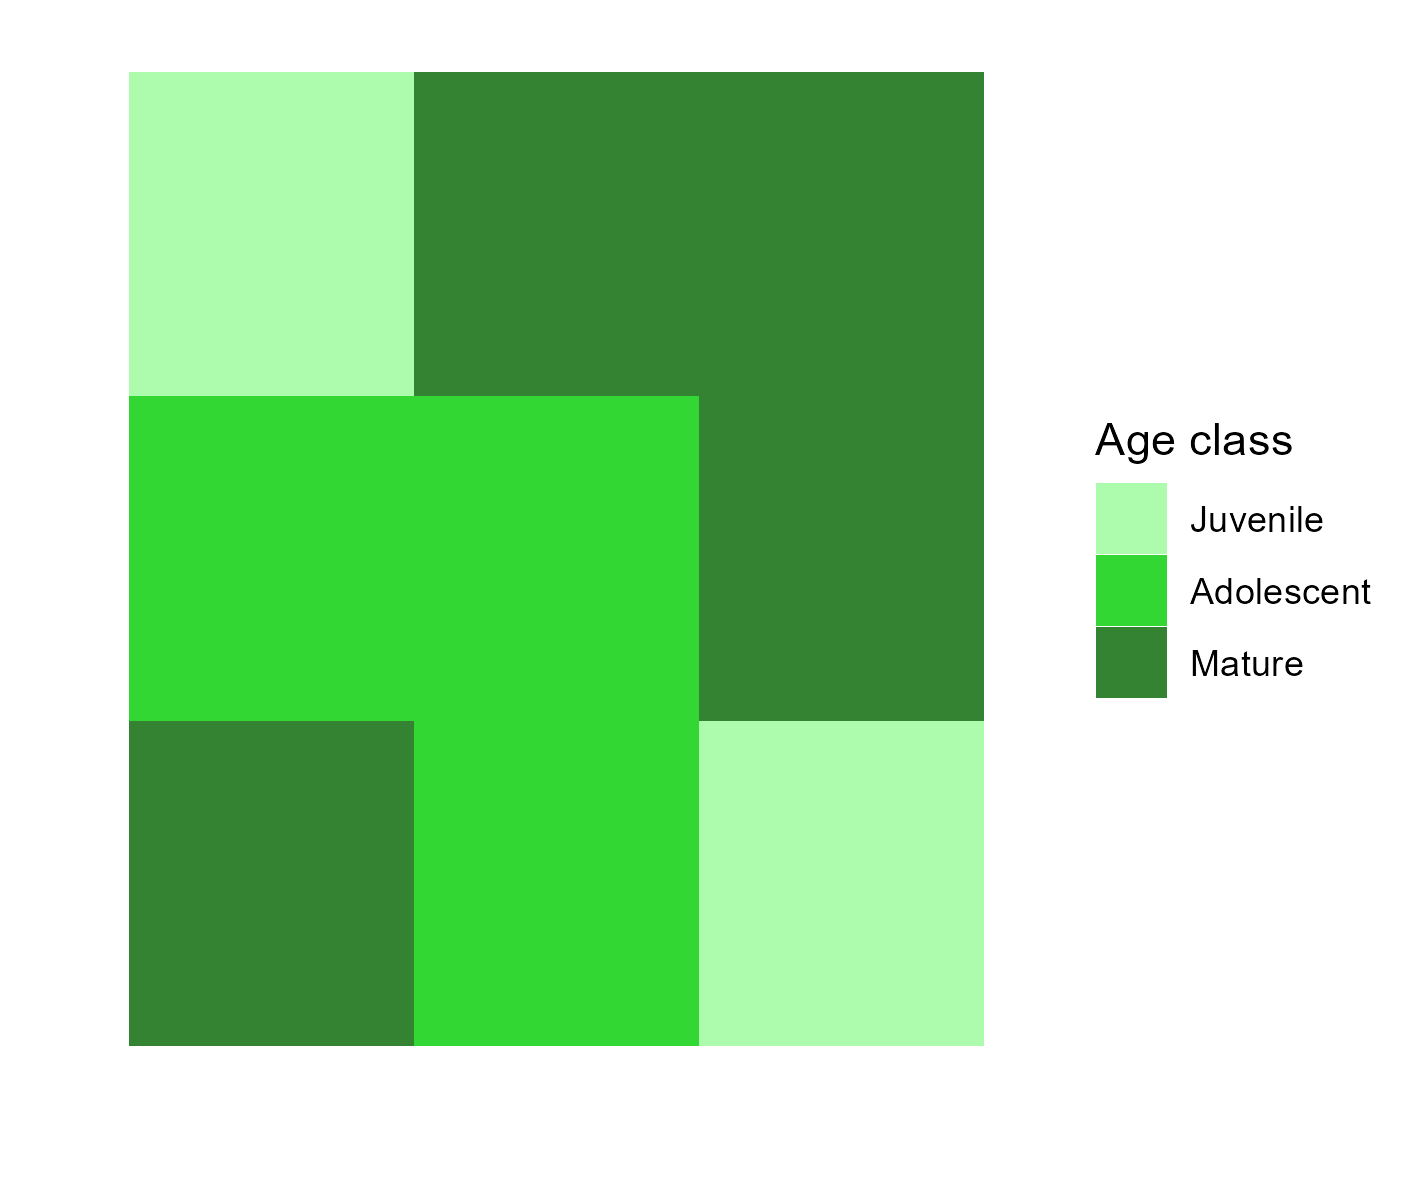
\includegraphics[width = .28\textwidth]{figures/wildland/illustration_from_raster.png}\\
    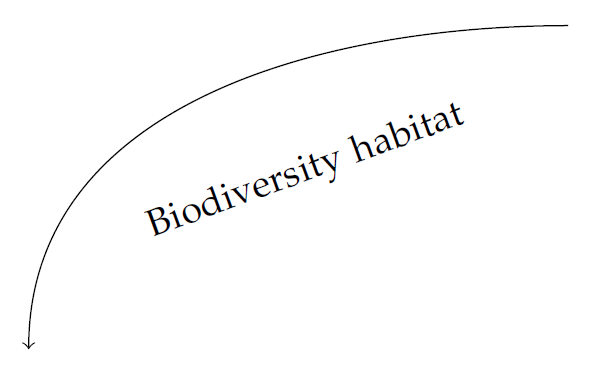
\includegraphics[width = 0.2\textwidth]{figures/wildland/arrow_biod2.PNG}
    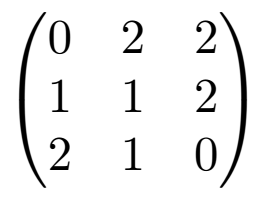
\includegraphics[width = 0.18\textwidth]{figures/wildland/land3.PNG}
    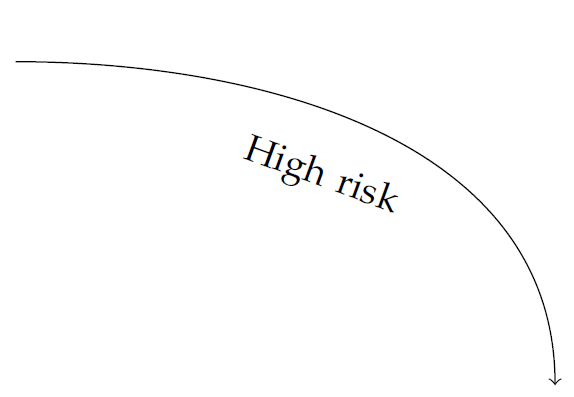
\includegraphics[width = 0.2\textwidth]{figures/wildland/arrow_fuel2.PNG}
    \\
    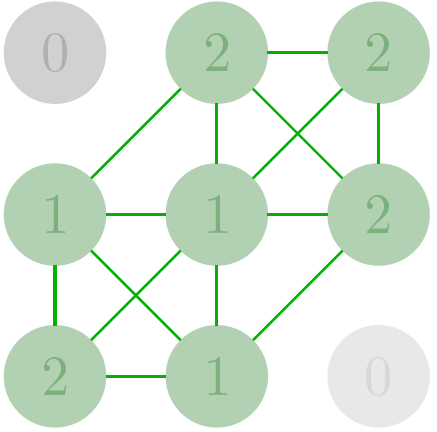
\includegraphics[width=0.2\textwidth]{figures/wildland/biodiv_3.PNG} \hspace*{4cm}
    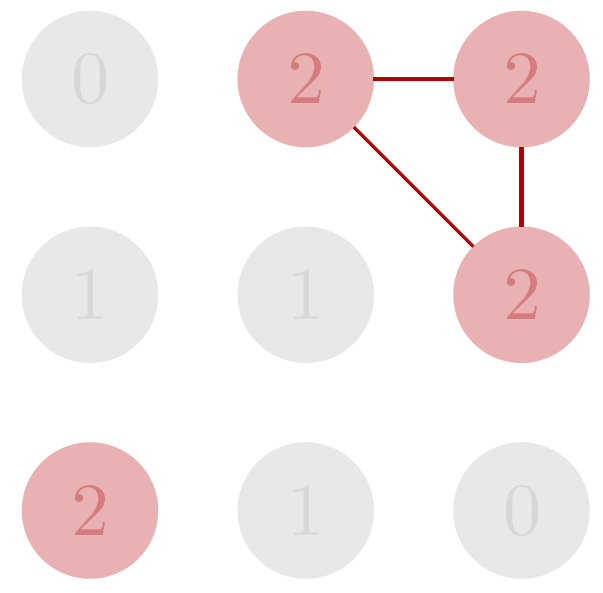
\includegraphics[width=0.2\textwidth]{figures/wildland/fire_3.PNG}\\
    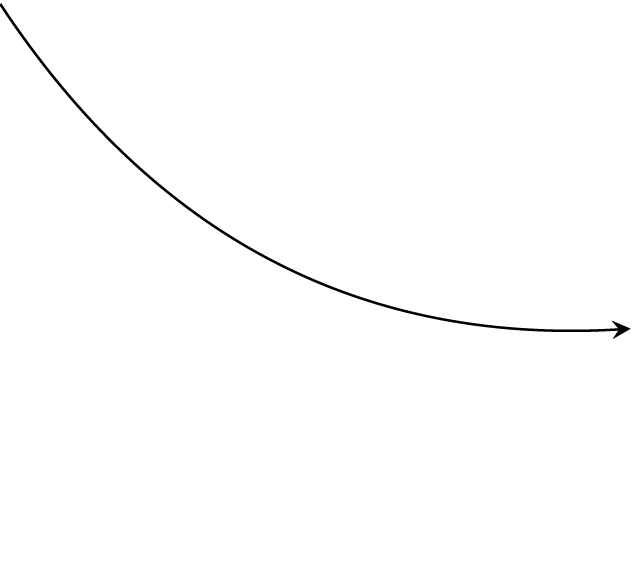
\includegraphics[width=0.18\textwidth]{figures/wildland/arrow_right.PNG}
    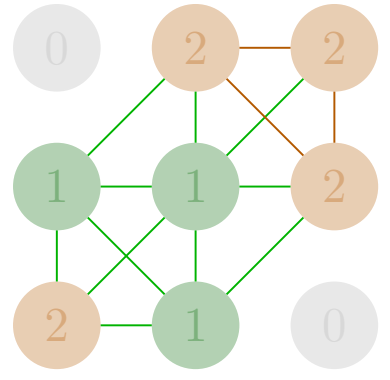
\includegraphics[width = 0.2\textwidth]{figures/wildland/graphe_feu_biod_33.PNG}
 	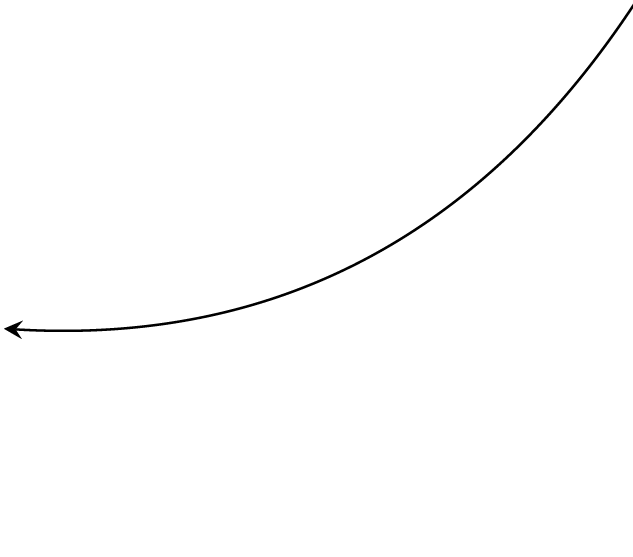
\includegraphics[width=0.18\textwidth]{figures/wildland/back_left.PNG}
    \caption{Illustration of the suitable habitat and high risk graphs for $n=3$}
    \subcaption*{The first layer is the values from a raster $\mathbf{A}_t$ of age classes in a forest landscape. It is turned into two different graphs. \\
In the left graph, the green vertices are $V_{\mathcal{B}_t}$ and support biodiversity habitat, while on the right graph, red vertices are $V_{\mathcal{F}_t}$ display high risk. Green and red links are respectively $E_{\mathcal{B}_t}$ and $E_{\mathcal{F}_t}$ \\
The high risk graph has two components (top right corner with 3 nodes, and bottom left corner with 1 node), while the biodiversity habitat graph only has one. \\
Cells for which the value is 0 are not considered as nodes for both graphs, and are thus not connected to the rest of the graphs. 
\\
In the final lansdcape, because $\mathcal{F}_t\subset \mathcal{B}_t$, the landscape  where orange cells are high fuel load and also support biodiversity habitat (e.g. $a_{ijt} \in V_{\mathcal{B}_t} \cap V_{\mathcal{F}_t}$)}
    \label{fig:graph_overlap}
\end{figure}

To assess the connectivity of $\mathcal{F}_t$ and $\mathcal{B}_t$, we use a global connectivity indicator. As connectivity can be measured in numerous ways in graph theory, we use this metric as is satisfies criteria pertaining to its evolution when vertices and edges are removed \citep{pascual-hortal_comparison_2006} when using graph theory applied to landscape ecology. Additionally, it offers a reformulation of the metric used in previous work closedly related to ours \citep{minas_spatial_2014, rachmawati_optimisation_2016} (see appendix \ref{sec:connectivity} for a demonstration). We define the global connectivity index of a given graph $\mathcal{G} = (\mathcal{V}, \mathcal{E})$ as\footnote{With $card$ being the cardinal operator in set theory and denotes the number of elements in a set}:
\begin{equation}
H(\mathcal{G}) = card(V) + 2card(E)
\label{eq:high_connectivity}
\end{equation} 
Let a \textit{patch} be a collection of connected cells of suitable wildlife habitat.
This indicator considers that a habitat cell is connected to itself (i.e, within a habitat patch, there is no barrier) and whether it is connected to other cells.  
It implies lower connectivity when the distance between habitat cells increases, attains its maximum value when a single habitat patch covers the whole landscape, indicates lower connectivity as the habitat is progressively more fragmented, considers negative the loss of a connected or isolated cell, and detects as more important the loss of bigger patch, and less important steppingstone cells or patches. 
\\
Our global connectivity indicator is similar to the notion of \textit{energy of a graph} \citep{gutman_energy_2001}, which can be understood as a measure of connectedness (highly connected graphs tend to have high energy) for graphs. However, we differ from \cite{gutman_energy_2001} by including self-loops as habitat cells and patches are connected to themselves. Our formulation of $H$ reframes a quadratic form from the adjacency matrix of a graph grid structure (appendix \ref{sec:connectivity}). The adjacency matrix displays interaction among nodes that are neither purely constructive or destructive, as some combinations of active neighboring nodes will add to global connectivity, while other combinations may substract global connectivity. In all the landscape sizes we used, eigenvalues of the adjacency matrix were both positive and negative, leading to indefiniteness (see figure \ref{fig:eigenvalues}). Therefore, $H$ is not globally convex nor concave. 
\\
%and The vertices of $\mathcal{B}_t$ are cells that are at suitable habitat status (e.g. $Habitat(a_{it})=1$ and high risk status (e.g. $Risk(a_{it})=1$) and suitable habitat status
%
%We transform $A_t$ the set of cells constituting the landscape into graphs $G_t$ whose vertices $V_t$ (or nodes) are the cells in the landscape, and edges $E_t$ represent the connections between cells. We partition the landscape in two graphs, $G_{B_t}$ and $G_{F_t}$, each describing the network of mature habitat and risky patches (see fig. 1 for a representation). Landscape ecology has long used numerous, theoretically grounded indicators to analyze landscapes 
%
%\citep{urban_landscape_2001,minor_graph-theory_2008}. We use a global connectivity indicator that satisfies \cite{pascual-hortal_comparison_2006} criteria, grounded in graph theory, that offer a reformulation of \cite{rachmawati_optimisation_2016} (see Appendix \ref{sec:connectivity}). 
%Figure reference : \ref{fig:graph_overlap}
%
%We define cells to be connected if (i) they are within an 8-cell neighborhood and (ii) share the same status e.g. for a cell $i$, if cell $j$ is an 8-cell neighborhood (should we define it?)
%
%We define the global connectivity index of habitat and risky patches in landscape $A(t)$ as:
%
%This indicator considers that a habitat patch is connected to itself (i.e, within a habitat patch, there is no barrier) and whether it is connected to other patches.  
%It implies lower connectivity when the distance between patches increases, attains its maximum value when a single habitat patch covers the whole landscape, indicates lower connectivity as the habitat is progressively more fragmented, considers negative the loss of a connected or isolated patch, and detects as more important the loss of bigger patches, of key and less important steppingstone patches.
%
%We use a connectivity matrix to evaluate the ladnscape such that ...
%\textit{note that the framework is robust to changing the dispersal abilities. For example, one could think of (i) changing the dispersal abilities and (2) increase the size of the landscape to run applied stuff and (3) finding metrics to prioritize over species with different dispersal abilities. \textbf{This is a good discussion point : next work should include a variety of dispersal abilities and contributions to functional diversity to really dig deeper in this issue. }}
%\\\\

\subsection{Social planner decision : the high-risk /connectivity dilemma}
\subsubsection{Dynamic decision problem}
A social planner tries to minimize the global connectivity index of the high risk graph, using fuel treatments (eq. \ref{eq:objective}). However, when implementing treatment, a cell's successional stage is reset to \textit{juvenile}, thus destroying biodiversity habitat. In coherence with real world applications, the social planner is faced with a temporal budget constraint (e.g. the sum of treatments $\sum_{ij}x_{ijt}$ must be lower or equal to the $Budget$ - eq. \ref{const:budget}) as well as an ecological constraint, in terms of biodiversity habitat connectivity (e.g. the global connectivity of biodiversity habitat $H(\mathcal{B}_t)$ must be larger than constraint $Biod$ - eq. \ref{constr:biod}). Both the ecological and budget constraint need to be satisfied in each period.
\\
For the sake of the analysis, we focus on two layers of complexity : time and space. We do not include a stochastic component related to wildfire risk e.g. we adopt a deterministic framework where the value at risk (global connectivity of risky cells) is weighed against the loss in biodiversity habitat connectivity. Additionally, we consider a homogeneous distribution of treatment costs across the landscape e.g. cost of treatment in each cell through time is $1$. We come back to this assumption in the discussion. Monetary benefits are also homogenously distributed across the landscape, and normalized to 1. Note that there is, however, heterogeneous returns to treating across the landscape : some cells will contribute more than other to global connectivity. Finally, given that the planning horizon is finite, we do not discount future high risk connectivity scores and assume each period is equally important in decision making.

The optimization problem is : 

\begin{align}
    \min_{ \{\{x_{ijt}\}_{(i,j)}\}_{t=1}^T} & \left[ \sum_{t=1}^T H(\mathcal{F}_t)\right] \label{eq:objective}\\
\text{Such that: } & \notag \\
\mathbf{A}_0 &\text{ given} \label{eq:init_cond}\\
\forall t \in \{1, ..., T\} : & \notag \\
H(\mathcal{B}_t)&\geq Biod,\text{  }\label{constr:biod}\\
\text{ and }\forall (i,j) \in \{1,...,n\}   :& \notag \\
a_{ijt+1}& = \min((a_{ijt+1}(1-x_{ijt});2), \label{const:dyn}\\
 \sum_{i,j} x_{ijt} & \leq Budget,\text{  } \label{const:budget}\\
x_{ijt}&\in \{0,1\}\label{const:control}
\end{align}

\begin{table}[h]
\centering
\onehalfspacing
\begin{tabular}{|c|c|}
\hline
Notation & Concept \\
\hline \hline
$\mathbf{A}_t$ & Landscape matrix representing successional stage at time $t$ \\
$a_{ijt}$ & Cell $(i,j)$ of landscape with value $\in \{0,1,2\}$\\ 
$x_{ijt}$ & Treatment status $\in\{0,1\}$ of cell $(i,j)$ at time $t$ \\
$H$ & Global connectivity measure\\
$\mathcal{F}_t = (V_{\mathcal{F}_t}, E_{\mathcal{F}_t})$ & Graph of high risk cells\\
$\mathcal{B}_t = (V_{\mathcal{B}_t}, E_{\mathcal{B}_t})$ & Graph of suitable habit cells\\
\hline \hline
$Biod \in \{0,...,\max H(\mathcal{B})\}$ & Level of habitat global connectivity constraint\\
$Budget \in \{1,2,3,4\}$ & Level of the budget constraint\\
$n \in \{3,4,100\}$ & Size of the lansdcape\\
$c = 3$ & Number of age classes \\
$T \in \{5,10\} $ & Planning horizon\\
\hline 
\end{tabular}
\caption{Summary of model variables and functions}
\end{table}
%There are several reasons for this choice. First, the complexity of our problem is increasing in space and time, and in the number of initial conditions, as interpolation in a spatial setting is difficult given the behavior of our objective function. 
As common in the literature, we can express the budget as a share of land being treated ranging from 10\% to 33\% of the surface area (when $n=3$) and 5 to 25\% of the surface area (when $n=4$). These values encompass historical and projected policies in Australia \citep{burrows2013}, the United States \citep{GAO2019} and Southern Europe \citep{Fernandes2013}.
\\
Additionally, we solve the problem for a range of possible habitat connectivity values, ranging from $0$ to the maximum possible habitat connectivity for each landscape size $n$.

\subsubsection{Non-convexity and dimensionality curse}
Our problem can be classified as a \textit{critical node detection problem}, i.e, a problem of locating the vertices that best degrade our global connectivity metric $H(\mathcal{F}_t)$ \citep{ARULSELVAN20092193}. Problems of the critical node class are computationally difficult (e.g. NP - Hard) in a single graph \citep{ARULSELVAN20092193, matsypura_wildfire_2018}. Efficient heuristics to find near-optimal solutions exist and leverage perturbations around local solutions \citep{ARULSELVAN20092193, Zhou2017}. Compared to the canonical \textit{critical node detection} problem, our problem features a non-convex objective function, a budget constraint, and a constraint on habitat connectivity, which imposes a constraint on the supergraph of high risk cells. Given our constraints, the behavior of the global connectivity measure $H$, standard optimization techniques cannot be applied, and heuristics are required. \\
%We solve the dynamic, integer program of the landscape manager
In dynamic problems, a standard technique is dynamic programming \citep{Bellman}. Dynamic programming provides a temporal decomposition of the initial problem defined over $T$ periods, into $T$ recursive problems, as it relies on the 'optimality principle'\footnote{"An optimal policy has the property that whatever the initial state and initial decision are, the remaining decisions must constitute an optimal policy with regard to the state resulting from the first decision". (See \cite{Bellman}, Chap. III.3., p.83)"}. A value function $V$, mapping each possible state of the world e.g. $\mathbf{A}_t$ to the optimal value of the objective function along the planning horizon, is iterated upon to find the optimal policies $x_{ijt}^*(\mathbf{A}_t)$, i.e, the sequence of optimal treatments, and the optimal states $\mathbf{A}_t^*(\mathbf{A}_0)$ resulting from the optimal policies and the initial conditions.
However, it is impractical in our case. Our problem suffers a \textit{dimensionality curse} \citep{Bellman}. There are $3^{n^2}$ values for the state variables \footnote{Given that the landscape $\mathbf{A}$ is of size $n\times n$, and that each element of $a_{ij}$ can take $c=3$ values, there are $3^{n^2}$ landcape configurations possible} in each period and the specific nature of our objective function $H$, the habitat connectivity and budget constraints make interpolation of a value function impossible \footnote{As a matter of fact, with a large number of state variables e.g. a high-dimensional state space, methods such as adaptive sparse grids can be used towith smooth, continuous objective functions \citep{brumm_adaptive_2017} to circumvent the dimensionality curse. The fact that the input space is an $n^2$-dimensional binary Cartesian product and that $H$ is not globally convex hinder the use of such tools.}.
%To manage the expected damages resulting from wildfires, the land planner can decide to undertake specific treatments, in the form of a combination of controlled burns and/or mechanical thinnings. Upon treatment, we assume that vegetation age in the cell is reset to 'absent': the wildfire risk vanishes, but so does the habitat and its connection to surrounding cells. Given the tension between maintaining habitat and reducing wildfire risk, the land planner aims to minimize a deterministic measure of connectivity of the high fuel loads in the landscape while maintaining a given level of biodiversity habitat connectivity under a budget constraint, over a planning horizon of length $T$. 
%For the sake of the analysis, we focus on two layers of complexity over time and space: global connectivity of high risk and biodiversity habitat. We do not consider stochastic wildfire behavior\textbf{point on risk and expected utility? } , heterogeneity in the economic costs or benefits (i.e, homogeneous treatment costs and no patch-specific asset to protect). The framework is however amenable to such a prioritization. We also assume that the budget cannot be banked, and has to be utilized in each period, consistent with operational rules. Moreover, as the budget is constrained in each period, the measure of risk is bounded and the planning horizon is finite, we rule out discounting and assume each generation matters as much to the social planner. 
%We abstract from decision-making in a risky environment, as it has been extensively described in economics and decision theory \citep{Mouysset2013}. Moreover, we mimic the role of risk aversion by varying the level of habitat connectivity constraint the decision maker chooses. 
%If ignition is a binary process in each period, the probability of which is independent of the high-risk graph properties, our model can be viewed as minimizing an upper bound of the expected losses from wildfires (see appendix).


\subsection{Solution method and computational experiments}

Three key features of our problem hint that a dynamic (e.g. that optimizes the objective function over the whole planning horizon) and a repeated myopic solution (e.g. which optimizes the objective function in each period)  should be similar. The dynamics occur before the decision is made, therefore the decision maker has full knowledge about the state of the system. The dynamics are simplified and have relatively little depth, as we limit ourselves to 3 age classes. Finally, our intertemporal objective function is additively separable.

Our solution methods resorts to two key ingredients : optimization heuristics, and comparison between the dynamic and repeated myopic problem. \\
First, we circumvent the non-convexity of the global connectivity metric and the high dimension of the state space by using a genetic algorithm \citep{holland_adaptation_1975} (implemented in \textsf{R} with package \textit{GA} \citep{GA_2017}) for 300 randomly generated landscapes, with population size of $200$ and $250$ iterations. Genetic algorithms are especially suited for high dimensional, combinatorial search spaces\footnote{Here, the control variable is a $Tn^2 = 5n^2$ binary variable} and fare better than a brute force approach, or other heuristics (Particle Swarm Optimization or Simulated Annealing). 
\\
Then, we compare the performance of a 5-period objective function to a 5 period repetition of a static objective function. We trade the completeness of dynamic programming for a more manageable approach, where we compare these approaches for $696$ and $884$ randomly drawn landscapes of size $n \in \{3,4\}$. We sample the landscapes according to the distribution of possible landscapes (see figure \ref{fig:appendix_distribution}). As landscapes with large numbers of \textit{juvenile} and \textit{adolescent} cells are overrepresented, we impose that underrepresented possible landscapes are included at least 2 times in our sample, to disentangle composition (e.g. number of cells of each successional stage) from configuration (location of cells) effects.

 We focus $T=5$ planning horizon for several reasons. First, as the dynamic of our ecological processes comprises 3 stages, using a 5-period horizon allows for each cell to grow from its original stage to \textit{mature}, be treated, and revert to its original stage, e.g. allows for a full successional cycle to be performed. Second, a 5-period horizon corresponds to a long policy horizon, ranging from 25 years to 200 years \citep{mccoll_gausden_pathways_2019, thomas_wildlife_1979}.
Third, for our approach to be useful for policy making given that we abstract from stochastic modifications to the environment (e.g. occurence of wildfire, spread of invasive species increasing flamability at a given age etc), policies need to be forward looking with enough temporal depth to be relevant and be reevaluated with potentially new initial conditions resulting from environmental perturbations.\\
Next, we increase the size of our sample with repeated static optimization and temporal depth, to encompass all the possible landscape configurations for landscape size $n \in \{3, 4\}$, over the whole range of possible values for the biodiversity habitat constraint, over $T=10$ years. 
Of all the $3^{n^2}$ initial landscapes combinations possible, we only keep landscapes that are unique up to a permutation\footnote{That is to say, landscape $\mathbf{A}_0$ is included in the set of initial conditions $\mathcal{I}$ if and only if for any element $\mathbf{A'}_0$ in $\mathcal{I}$, $\mathbf{A}_0$ is not a permutation (eg can be obtained through rotations or symmetries) of $\mathbf{A'}_0$}. This results in a sharp reduction of landscapes to consider, from $19,683$ initial conditions to $2861$ unique initial landscapes for $n=3$, and from $43,046,721$ initial to $5,398,082$ unique initial landscapes for $n=4$. We focus on exact optimal solutions for all the initial conditions of these small-scale landscapes and implement our own solution algorithm in Python 3.9.13 and R 4.3.3\footnote{Data and code are \href{https://github.com/sim-jean/Landscape_connectivity_dilemma}{publicly available}}.
\\
Third, we increase the landscape size to $n=100$, for a sample of 20 large scale (10,000 cells) landscapes with varying compositions and autocorrelation using two-dimensional fractional Brownian motions  (table \ref{tab:composition_nlm} summarizes their characteristics and figure \ref{fig:ex_nlm} illustrates 6 of them). We use neutral landscape models \citep{caswell_community_1976, gardner_neutral_2007} and implement them in \textsf{R} \citep{sciaini_nlmr_2018}. Neutral landscape models were designed in theoretical landscape ecology to develop spatial ecology indicators and ``evaluate the effects of landscape structure on ecological processes'' \citep{with_neutral_1997}. Even though they are designed as null models to compare with real landscapes, after ecological processes have shaped them, they provide a useful basis for scaling our analysis. We solve the repeated myopic optimization problem on these 20 landscapes over $T=10$ periods.\\
%
%
%\subsubsection{Non-convexity and dimensionality curse}
%Our problem can be classified as a \textit{critical node detection problem}, i.e, a problem of locating the vertices that best degrade our global connectivity metric $H(\mathcal{F}_t)$ \citep{ARULSELVAN20092193}. Problems of the critical node class are computationally difficult (e.g. NP - Hard) in a single graph \citep{ARULSELVAN20092193, matsypura_wildfire_2018}. Efficient heuristics to find near-optimal solutions exist and leverage perturbations around local solutions \citep{ARULSELVAN20092193, Zhou2017}. Compared to the canonical \textit{critical node detection} problem, our problem features non-convex objective function, a budget constraint, and a constraint on habitat connectivity, which imposes a constraint on the supergraph of high risk cells. Given our constraints, the behavior of the global connectivity measure $H$, standard optimization techniques cannot be applied. \\
%We solve the dynamic, integer program of the landscape manager
%In dynamic problems, a standard technique is dynamic programming. Dynamic programming provides a temporal decomposition of the initial problem defined over $T$ periods, into $T$ recursive problems, as it relies on the 'optimality principle'\footnote{"An optimal policy has the property that whatever the initial state and initial decision are, the remaining decisions must constitute an optimal policy with regard to the state resulting from the first decision". (See \cite{Bellman}, Chap. III.3., p.83)"}. A value function $V$, mapping each possible state of the world e.g. $\mathbf{A}_t$ to its objective function value, is iterated upon to find the optimal policies $x_{ijt}^*(\mathbf{A}_t)$, i.e, the sequence of optimal controlled burns, and the optimal states $\mathbf{A}_t^*(\mathbf{A}_0)$ resulting from the optimal policies and the initial conditions.
%However, it is impractical in our case. As a matter of fact, our problem suffers a \textit{dimensionality curse} \citep{Bellman}. There are $3^{n^2}$ possible combinations\footnote{Given that the landscape $\mathbf{A}$ is of size $n\times n$, and that each element of $a_{ij}$ can take $c=3$ values, there are $3^{n^2}$ landcape configurations possible} in each period and the specific nature of our objective function $H$, the habitat connectivity and budget constraints make interpolation of a value function impossible \footnote{As a matter of fact, even with a large number of state variables e.g. a high-dimensional state space, adaptive sparse grids can be used with smooth, continuous objective functions \citep{brumm_adaptive_2017}. The fact that the input space is an $n^2$-dimensional binary Cartesian product and that $H$ is not globally convex hinder the use of such tools.}. 
%
%Nonetheless, three key features of our problem hint that dynamic and repeated myopic solutions should be similar. The dynamics occur before the decision is made, therefore the decision maker has full knowledge about the state of the system. The dynamics are simplified and have relatively little depth, as we limit ourselves to 3 age classes. Finally, our intertemporal objective function is additively separable.
%
%
%
%\subsubsection{Dynamic v. repeated myopic solutions}
% 
%To circumvent this issue, we adopt a three-fold approach. \\
%First, we trade the completeness of dynamic programming (e.g. solution of the problem for the entire domain of the state variable $\mathbf{A}$) for a manageable piecemeal approach, where we solve the complex 5-period combinatorial problem with a genetic algorithm \citep{holland_adaptation_1975} (implemented in \textsf{R} with package \textit{GA} \citep{GA_2017}) for 300 randomly generated landscapes, with population size of $200$ and $250$ iterations. Genetic algorithms are especially suited for high dimensional, combinatorial search spaces\footnote{Here, the control variable is a $Tn^2 = 5n^2$ binary variable} and fare better than a brute force approach, or other heuristics (Particle Swarm Optimization or Simulated Annealing). 
%
%Three key features of our problem hint that dynamic and repeated myopic solutions should be similar. The dynamics occur before the decision is made, therefore the decision maker has full knowledge about the state of the system. The dynamics are simplified and have relatively little depth, as we limit ourselves to 3 age classes. Finally, our intertemporal objective function is additively separable.
%Hence, we compare the performance of the 5 period, genetic algorithm approach to a repeated static optimization procedure, for landscapes of size $n\in\{3,4\}$. While this size appears simplifying, it encapsulates the main mechanisms displayed in similar models \citep{rachmawati_optimisation_2016, rachmawati_fuel_2018}. Based on these results, we increase the planning horizon to
%\\
%\textbf{Comment est ce qu'on dit ici qu'on accroit peut être l'horizon?}
%Second, we perform a repeated static optimization on all the possible landscape configurations for landscape size $n \in \{3, 4\}$, over all the whole range of possible values for the biodiversity habitat constraint, over 5 years. This approach sacrifices the dynamics of our problem but allows us to scan the entire state space to gain insights.
%Of all the $3^{n^2}$ initial landscapes combinations possible, we only keep landscapes that are unique up to a permutation\footnote{That is to say, landscape $\mathbf{A}_0$ is included in the set of initial conditions $\mathcal{I}$ if and only if for any element $\mathbf{A'}_0$ in $\mathcal{I}$, $\mathbf{A}_0$ is not a permutation (eg can be obtained through rotations or symmetries) of $\mathbf{A'}_0$}. This results in a sharp reduction of landscapes to consider, from $19,683$ initial conditions to $2861$ unique initial landscapes for $n=3$, and from $43,046,721$ initial to $5,398,082$ unique initial landscapes for $n=4$. We focus on exact optimal solutions for all the initial conditions of these small-scale landscapes and implement our own solution algorithm in Python 3.9.13 and R 4.3.3\footnote{Data and code are \href{https://github.com/sim-jean/Landscape_connectivity_dilemma}{publicly available}}.
%\\
%Third, we simulate 20 large scale (10,000 cells) landscapes with varying compositions and autocorrelation using two-dimensional fractional Brownian motions  (table \ref{tab:composition_nlm} summarizes their characteristics and figure \ref{fig:ex_nlm} illustrates 6 of them). We use neutral landscape models \citep{caswell_community_1976, gardner_neutral_2007} and implement them in \textsf{R} \citep{sciaini_nlmr_2018}. Neutral landscape models were designed in theoretical landscape ecology to develop spatial ecology indicators and ``evaluate the effects of landscape structure on ecological processes'' \citep{with_neutral_1997}. Even though they are designed as null models to compare with real landscapes, after ecological processes have shaped them, they provide a useful basis for scaling our analysis. We solve the repeated myopic optimization problem on these 20 landscapes.
%
%using dynamic programming. Dynamic programming provides a temporal decomposition of the initial problem defined over $T$ periods, into $T$ recursive problems, as it relies on the 'optimality principle'\footnote{"An optimal policy has the property that whatever the initial state and initial decision are, the remaining decisions must constitute an optimal policy with regard to the state resulting from the first decision". (See \cite{Bellman}, Chap. III.3., p.83)"}.  The outputs of the method are both the optimal policies $x_j^*(t,A)$, i.e, the sequence of optimal controlled burns, and the optimal states $A_j^*(t,A_0)$ resulting from the optimal policies and the initial conditions. Moreover, we solve a repeated myopic optimization procedure, where in each time step, the decision maker minimizes the current global connectivity measure of high risk cells, under constraints \ref{eq:init_cond}-\ref{const:control}. In the dynamic problem, the biodiversity habitat and budget constraints gradually restrict the solution space, and limit the extent to which system dynamics (e.g the appraisal of long terms successional stages across the landscape) may impact optimal solutions. We compare the repeated myopic solution to the dynamic solution.
%
%\subsubsection{Circumventing non-convexity and dimensionality curse}
%
%Our problem can be classified as a \textit{critical node detection problem}, i.e, a problem of locating the vertices that best degrade our global connectivity metric $H(\mathcal{F}_t)$ \citep{ARULSELVAN20092193}. Problems of the critical node class are computationally difficult (e.g. NP - Hard) in a single graph \citep{ARULSELVAN20092193, matsypura_wildfire_2018}. Efficient heuristics to find near-optimal solutions exist and leverage perturbations around local solutions \citep{ARULSELVAN20092193, Zhou2017}. Our problem is a constrained, integer optimization problem with a non-convex objective function,
%that constrains not only the set of nodes to be removed but also metrics relative to a larger graph structure e.g. the supergraph of high risk cells, biodiversity habitat. Given the behavior of the global connectivity measure $H$, standard optimization techniques cannot be applied. \\
%Additionally, the complexity of our combinatorial problem increases with landscape size $n$, the number of vegetation age classes $c$, and time $T$ i.e. features a \textit{dimensionality curse} \citep{Bellman}: there are $c^{n^2}$ eg. $3^{n^2}$ initial landscape configurations possible, and given an initial landscape, there are $n^2 \times T$ possible treatment allocations to be considered. 
%To circumvent these issues, we use a genetic algorithm \citep{holland_adaptation_1975} (implemented in \textsf{R} with package \textit{GA} \citep{GA_2017}). Compared to other heuristics, such as Particle Swarm Optimization or Simulated Annealing, genetic algorithms fare better on high dimension, combinatorial search spaces. With small scale landscapes (e.g. $n\in \{3,4\}$), we use a population size of $100$ individuals with $250$ iterations which guarantees that the heuristic converges to a near optimal solution.
%
%Moreover, as the objective function is neither globally convex nor concave, and the structure of the optimization problem is constrained, we required large test populations for our genetic algorithm to avoid getting stuck in local minima.  es.
%
%\subsubsection{Small and large scale repeated myopic optimization}
%
%We limit ourselves to studying the initial conditions in landscapes of size $n=3$ and $4$. While this formulation appears simplifying, it encapsulates the main mechanisms displayed in similar models \citep{rachmawati_optimisation_2016, rachmawati_fuel_2018}.\\
%First, we solve the dynamic problem and repeated static problem for 300 randomly selected initial landscapes.
%Then, we focus on all the possible landscape combinations of size $n \in \{3,4\}$ using repeated myopic optimization, over all the whole range of possible values for the biodiversity habitat constraint, over 5 years. \\
%Of all the $3^{n^2}$ initial landscapes combinations possible, we only keep landscapes that are unique up to a permutation\footnote{That is to say, landscape $\mathbf{A}_0$ is included in the set of initial conditions $\mathcal{I}$ if and only if for any element $\mathbf{A'}_0$ in $\mathcal{I}$, $\mathbf{A}_0$ is not a permutation (eg can be obtained through rotations or symmetries) of $\mathbf{A'}_0$}. This results in a sharp reduction of landscapes to consider, from $19,683$ initial conditions to $2861$ unique initial landscapes for $n=3$, and from $43,046,721$ initial to $5,398,082$ unique initial landscapes for $n=4$. We focus on exact optimal solutions for all the initial conditions of these small-scale landscapes and implement our own solution algorithm in Python 3.9.13 and R 4.3.3\footnote{Data and code are \href{https://github.com/sim-jean/Landscape_connectivity_dilemma}{publicly available}}.
%
%
%
%Finally, we simulate 20 large scale (10,000 cells) landscapes with varying compositions and autocorrelation using two-dimensional fractional Brownian motions  (table \ref{tab:composition_nlm} summarizes their characteristics and figure \ref{fig:ex_nlm} illustrates 6 of them). We use neutral landscape models \citep{caswell_community_1976, gardner_neutral_2007} and implement them in \textsf{R} \citep{sciaini_nlmr_2018}. Neutral landscape models were designed in theoretical landscape ecology to develop spatial ecology indicators and ``evaluate the effects of landscape structure on ecological processes'' \citep{with_neutral_1997}. Even though they are designed as null models to compare with real landscapes, after ecological processes have shaped them, they provide a useful basis for scaling our analysis. We solve the repeated myopic optimization problem on these 20 landscapes.
%
%
\subsection{Lanscape indicators}
\label{section:indicators}
To characterize the managed landscapes, we mobilize several indicators from landscape ecology and graph theory (see appendix \ref{sec:appendix_wildland__indicators}).

First, we account for the high risk and habitat surfaces in the landscape by measuring the number of vertices in each graph.
Second, to assess landscape connectivity and fragmentation as well as landscape diversity\footnote{In the context of fire prone ecosystems, the notion of ``fire mosaics'' \citep{bradstock_which_2005} conveys the idea that fire causes variations in successional stages through space thus providing different types of habitat for biodiversity and improving biodiversity}, we use our global connectivity metric $H$ (eq. \ref{eq:high_connectivity}), as well as the \textit{number of components}\footnote{A \textit{component $\mathcal{C}_t$} of graph $\mathcal{G}_t$ is a maximally connected subgraph of $\mathcal{G}_t$ that is not part of any larger connected subgraph. A component is \textit{connected} (for all two vertices $(u,v) \in V_{\mathcal{C}}$, there exists a path in $\mathcal{C}_t$ that connects them) and $\mathcal{C}_t$ being a subgraph of $\mathcal{G}_t$, it is \textit{maximal} if there is no other connected subgraph $\mathcal{C'}$ of $\mathcal{G}_t$ such that $\mathcal{C}_t$ is a proper subgraph of $\mathcal{C'}_t$. Figure \ref{fig:graph_overlap} illustrates this concepts in both the habitat and high risk graphs resp. $\mathcal{B}_t$ and $\mathcal{F}_t$}.
To specifically assess landscape diversity, we use the Simpson index \citep{simpson_measurement_1949} on successional stages stages (eq. \ref{eq:simpson})\footnote{Similar results can be found with the Shannon index \citep{Shannon1949}. To avoid issues related to degenerate values and logarithms, we focus on the Simpson index.}. 
However, the Simpson index does not account for the diversity of spatial patterns: a checkered landscape with two seral stages would be as diverse as a landscape with two large patches for each seral stage, according to the Simpson index. Therefore, we use the landscape shape index (eq. \ref{eq:LSI}), a normalized ratio between the perimeter of biodiversity habitat and its area \citep{patton_diversity_1975, McGarigal_1995}.
%\begin{equation}
%LSI = \frac{perimeter(\mathcal{G}_t)}{4n} \text{ such that }\mathcal{G}_t \in \{\mathcal{B}_t,\mathcal{F}_t\}
%\end{equation}
To disentangle the correlated effects of perimeter and area that affect the landscape shape index, we use a successional stage heterogeneity index, that averages the probability that, for each cell, neighbors in the 4 cardinal directions share the same successional stage (eq. \ref{eq:lth_index}). The index ranges between 0, when the successional stage is the same across the whole landscape, to 1, in a checkered landscape. The index assesses whether the landscape is a mosaic \citep{bradstock_which_2005}, and if it displays structural diversity, conducive to diverse communities and functional diversity. 

\section{Results}
\label{section:results}
\begin{itemize}
\item Need to rethink the argument in terms of steady states
\\
$\Rightarrow$ We no longer can use this argument because we sacrificed the duration
\item We want to characterize the long term trajectories with $T=5$?
\item What can we do?
\end{itemize}
\subsection{Steady states}
Our simulations show that 100\% of the initial landscapes converge in finite time towards a steady state solution, that minimizes wildfire risk while satisfying budgetary and habitat connectivity requirements. Steady states are landscape cycles with finite periods. Analyzing the steady-state cycles (and the unique landscapes that form them) drastically reduces the set of landscapes to analyze: they represent 2\% (resp. $0.001\%$) of the initial landscapes of size $n=3$ (resp. $n=4$). Our model highlights the convergence of landscapes towards types that can be managed to deliver several objectives. As landscape size increases, the number of steady state landscape cycles increases, but the power of convergence increases as well (e.g. ratio between initial configurations and effective steady state landscapes): from 19 683 initial landscapes when $n=3$, 51 steady states emerge and from 43 046 721 initial landscapes when $n=4$, at most 95 diverse steady-state landscapes emerge. Focusing on steady states makes all the more sense as landscape size increases. 

Eventually, figure \ref{fig:distrib_cycles} shows that conditional on data availability on every patch, the more the decision maker wants to conserve biodiversity, the fewer steady-state landscapes she has to consider. An increase in the habitat requirement reduces the room for maneuver. Indeed, budget acts as a complexifying factor: the larger the budget (relative to costs), the larger the set of steady-states to consider. 
%Our results show that habitat connectivity can be an objective and serve as an information cost-saving strategy. Data on the status of land patches gets cheaper to acquire with remote-sensing strategies, and random environmental factors can perturb optimal trajectories.
Aiming for relatively large habitat connectivity reduces the set of viable strategies to be considered and can more efficiently guide policy. 

\subsection{Wildfire risk reduction and habitat connectivity in steady state landscapes}

Figure \ref{fig:frontier} shows the wildfire risk reductions and habitat requirements normalized by their respective maximum values for landscapes of size $n=3$ and $4$. The maximum value for both risk and habitat corresponds to a landscape covered in 'old' vegetation, which we take to be the counterfactual. 
Randomly assigned treatments do generate risk reductions but are not cost nor habitat-efficient. Following our spatial optimization procedure, it is clear that implementing fuel treatment reduces wildfire risk while supporting biodiversity habitat. Figure \ref{fig:frontier} shows that these two objectives come as a trade-off, albeit moderate: indeed, increasing habitat requirements increases the remaining risk, but there are combinations that can satisfy large habitat connectivity and risk reductions. 
Budget is a key factor in risk reduction, as it relaxes the trade-off between the two objectives: increasing the budget reduces the wildfire risk while maintaining a range of biodiversity constraints. When habitat constraints are large, however, the marginal effect of budget is limited, and a larger remaining risk needs to be accepted. For example, with a budget of 25\% of land to be treated (with landscape size $n=4$), and no habitat constraint, risk can be reduced up to 80\% compared to the counterfactual scenario. However, when the habitat constraint is at 60\%, only 70\% of risk reduction can be achieved. Moreover, this risk reduction can be achieved with a lower budget. Conversely, as the costs of treatment increase, for a stable budget, the remaining risk increases sharply, and factoring in habitat requirements in the decision-making is not necessary for targets below 80\%. 
%\textbf{Pas sur de ça, un peu gros peut être?} Our results suggest that in the face of climate change if treatment costs increase, focusing on reducing wildfire risk should be a priority and would accommodate wildlife habitat. 
%\textbf{Point sur l'importance de la spatialisation? i.e, meilleur score vs random? ou focus sur un seral stage?}

\subsection{Properties of steady state landscapes: surface, fragmentation, and diversity}
Figure \ref{fig:cycles_3_4} displays, for each class, the most frequent steady-state cycle for landscapes of size $3$ and $4$ for each biodiversity target. 
%Figures \ref{fig:indicators_1} and \ref{fig:indicators_2} show the indicators (detailed in section \ref{section:indicators}) averaged over all the steady-state landscape cycles. 
Figure \ref{fig:indicators_1} shows the indicators relative to the surface and components of the high-risk graph and figure \ref{fig:indicators_2} shows the indicators related to diversity, both for landscapes of size $n=3$ and $4$, averaged over all the steady-state landscape cycles. 


Previous results show that budget increases risk reduction, conditional on habitat connectivity constraint being low. Focusing on zones $A$ and $A'$ of the panels of figure \ref{fig:indicators_1} shows that risk reduction primarily comes from a reduced surface (panels \ref{fig:indicator_surface3} and \ref{fig:indicator_surface4}), and an increase in the number of components, i.e, disconnected high-risk patches (panels \ref{fig:indicator_component3} and \ref{fig:indicator_component4}). Overall, the high-risk area is reduced and the number of components increases, thus resulting in smaller largest high-risk component area (panels e and f). As more connected habitat area needs to be protected, the high-risk surface increases (fig. \ref{fig:cycles_3_4} panels \ref{fig:indicator_surface3} and \ref{fig:indicator_surface4}) and the number of high-risk components drastically reduces. The landscapes collapse to the same dominant structure (fig. \ref{fig:cycles_3_4}), where the high-risk area is (almost) maximal and there is one large, well-connected component.  Overall, landscapes are riskier but also feature larger, better-connected biodiversity habitat. For large budgets (e.g. $3$ and $4$), these effects are non-trivial: the number of components (weakly) increases first, small components either disappear or increase in size (see figure \ref{fig:cycles_3_4} for budget $4$ in panels $A', B'$ and $C'$), risky patches are reallocated to connect separated components before the high-risk surface increases. 

Landscape diversity unambiguously increases with the budget (panels \ref{fig:indicator_simpson3},\ref{fig:indicator_simpson4}, sections $A$ and $A'$). As more units are treated, the evenness of seral stages increases in the landscapes. When the habitat objective is low, the spatial diversity of landscapes increases with the budget (panels \ref{fig:indicator_LSI3}, \ref{fig:indicator_LSI4}): even though the relative area of habitat decreases with the budget, the shape of habitat is more irregular, and the landscape is more of a mosaic. In this context, cells with a 'young' seral stage act as stepping stones and corridors between high-risk habitat patches. When habitat objectives increase, diversity collapses both quantitatively and qualitatively (fig. \ref{fig:indicators_2}). The Simpson index collapses from panels $A$ (resp. $A'$) to $G$ (resp. $F'$), as land types gradually homogenize (see fig. \ref{fig:cycles_3_4} for an illustration) across all budgets. Moreover, landscapes form less of a mosaic, and are more clumpy, as displayed by the LSI and Land type heterogeneity index. Overall, for large habitat targets, landscapes tend to homogenize and to be better connected, although less quantitatively and qualitatively diverse. 

Results are consistent across landscape sizes while they display more variability for size $n=3$, as border effects play a larger role. 
%\begin{enumerate}
%    \item Budget
%    \begin{itemize}
%        \item When budget is large, we have seen that risk is low(er). How?
%        \item The overall area is lower when budget is large  : more cells are being treated. 
%        \item Moreover, the number of disconnected subgraphs tends to increase, as the budget increases : the wildfire risk is fragmented and spread on the landscape (unless the budget is large enough that only 1 small component remains in the landscape for case 3)
%        \item Moreover, the size of at risk components decreases with budget. 
%        \item \textbf{Need to find the angle for diversity} : diversity increases with budget, as more patches can be treated (simpson and shanon). From a spatial perspective, for a lax requirement, it also increases diversity, where diverse patch are well connected to the rest of the lansdcape. It is a well connected diversity because the LSI is large. 
%    \end{itemize}
%    \item Habitat constraint 
%    \begin{itemize}
%        \item As biodiversity connectivity requirements increase, the risky area increases, and the number of components tends to decrease : more habitat patches need to be connected. 
%        \item Interestingly, there is a trade-off between : adding 1 patch (vertex) to a component such that it is not connected with the rest of the graph, or not adding one, but such that it connects components. 
%        \item \textbf{Framing here} : diversity tends to decrease with biodiversity requirement, both quantitatively and qualitatively
%        \begin{enumerate}
%            \item Find story for the lower budget above the larger for LSI : more area in lower budget, so maybe that's overall better. 
%            \item Fit a discussion point : our metric focuses on a single species, and we show that id functional diversity needs to be accounted for, then single species habitat is not the right metric
%        \end{enumerate}
%    \end{itemize}

%\end{enumerate}


\subsection{Spatial allocation of optimal management at the steady-state landscape cycle}
Figures \ref{fig:treatments_number3} and \ref{fig:treatments_number4} display the number of fuel treatments in the steady-state cycles, for various budgets and habitat connectivity constraints. 
Treatment allocation follows the evolution of the high-risk area (fig \ref{fig:indicator_surface3} and \ref{fig:indicator_surface4}): the larger the budget, the larger the treated area, the budget constraint is always satiated. However, when biodiversity targets increase, the budget constraint is no longer satiated.

Figures \ref{fig:treatments_pattern3} and \ref{fig:treatments_pattern4} display the average spatial location of treatments in the steady state cycles. The darker the cell, the higher the frequency of treatment. First, not all cells are equally treated. For low levels of biodiversity constraint, panels $A$ and $A'$ of figures \ref{fig:treatments_pattern3} and \ref{fig:treatments_pattern4} show that central cells are primarily treated, and when the budget increases, cells on the edges get treated, while corner cells are never treated. In the context of critical node detection, when the ecological requirements are low, the high-risk graph is primarily considered, and nodes with the most cost-efficient risk reduction, i.e, with the largest degree are targeted. Once the most connected cells are treated, lower-degree cells get treated. 

When habitat constraints increase, several effects come at play. Not only does the number of treatments decrease, but the spatial allocation also changes. For example, in panels $A$ and $B$ for budgets $3$ and $4$, panels $C$ and $D$ for budget $2$ and panels $E$ and $F$ for budget $1$ in figure \ref{fig:treatments_pattern3}, the number of treatment remains the same but is spatially reallocated to lower degree nodes. Treatments are spatially reallocated before being reduced. In this context, as the relative weight of the habitat graph increases, treating the most cost-efficient risk-reducing nodes also degrades habitat connectivity. Therefore, as habitat targets increase, edge and corner (e.g. low degree nodes) are being treated and habitat connectivity is maintained.


%\renewcommand{\arraystretch}{2}
%\begin{table}[h]
%   \centering
%   \resizebox{.7\textwidth}{!}{
%    \begin{tabular}{|c|c|c|c|}
%    \hline \hline
%         & \textbf{Habitat target} & \textbf{Low} & \textbf{Large} \\
%    \hline
%     \textbf{Budget}    &  \textit{Number of treatments} & \multicolumn{2}{c|}{\textit{Decreasing}}\\
%    \hline
%   \textbf{Low} & \multirow{3}{*}{\textit{Increasing}} & Most central nodes   & Edges and corners\\
%   \cline{3-4} \cline{1-1}  
%     \textbf{Large} & & Most central nodes  & Less central nodes,\\ 
%      & & and lower degree nodes &  edges and corners\\
%     \hline \hline
%    \end{tabular}}
%    \caption{Spatial treatment allocation in landscapes $n=3,4$}
%    \label{tab:synth_treatments}
%\end{table}


\section{Discussion}
\label{section:discussion}

\subsection{Confirmation and generalization of existing results}
Our analysis of the exhaustive set of initial conditions for small-scale landscapes confirms existing results in the literature. We argue that they bring robust evidence and complement the existing literature to derive general conclusions. 

Our model encompasses 3 seral stages and 1 composite vegetation type and proves the convergence of every initial condition to a steady state cycle, irrespective of the initial configuration. We extend \cite{minas_spatial_2014} that find convergence patterns for \textit{homogeneous} landscapes only, i.e, landscapes where the initial vegetation age is uniformly distributed.  We show that in the event of environmental perturbations that do not disrupt ecosystem dynamics, an appropriate policy can recover the previous equilibrium risk and habitat.
We hypothesize that as long as the risk/ seral-stage relationship reaches a plateau for every vegetation type on the landscape, convergence should be observed.

Our results display a concave production possibility frontier (PPF) between wildfire risk reduction and habitat connectivity, consistent with PFF literature \citep{arthaud_methodology_1996,calkin_modeling_2005}. Our results also confirm that trading one objective for the other is not as efficient as increasing the policy budget to reconcile objectives. We show that increasing the policy budget nonetheless has diminishing returns for risk reduction, as highlighted by \cite{wei_optimization_2008, yemshanov_detecting_2021} and \cite{pais_cell2fire_2021}. 

Our study yields clear results in terms of landscape ecology, leveraging concepts from landscape ecology, and highlighting the spatial mechanisms underlying the shape of PPF. We show that treatment allocation targets the most central nodes first and then focuses on less connected nodes (e.g cells closer to the border of the landscape) when habitat goals are low. In doing so, we do find general treatment allocation principles where previous studies on larger landscapes could not \citep{minas_spatial_2014, rachmawati_optimisation_2016}, generalize smaller scale \citep{konoshima_spatial-endogenous_2008} and case study specific \citep{yemshanov_detecting_2021, pais_downstream_2021} results.

%In \cite{minas_spatial_2014}, the authors advocate that general patterns are difficult to identify with larger landscapes and more heterogeneous distributions of initial vegetation age. Nonetheless, conditional on the location of potential treatments, it is clear that the allocation first targets central cells, and then focuses on cells closer to the edges of the landscape. In \cite{rachmawati_optimisation_2016}, treatments are allocated in priority to the center of the landscape, and as fewer treatment zones are available, to the edges of the landscape. 
%In articles further from our set-up, which do not leverage graph theoretic tools, we find consistent results. 
%For example, in \cite{konoshima_spatial-endogenous_2008}, the authors look at a theoretical forest comprised of hexagonal stands, where wildfire risk decreases with age but the value of timber increases with age. The land planner has to choose if, or when, to harvest, and if or when to treat the stands. As this framework is symmetric to ours, they achieve comparable results on smaller landscapes. Indeed, as the value at loss increases, treatments focus management units with large spread rates, on the center unit, and to cells in the middle of what could connect wildfire components. In articles explicitly leveraging graph theory, such as in \cite{matsypura_wildfire_2018}, they show that using degree optimization yields the largest reduction in wildfires, and that conditional on being treatable, the treatments are allocated to the largest degree nodes. These results are consistent with other studies such as \cite{yemshanov_detecting_2021} or \cite{pais_downstream_2021}. 
Leveraging a dynamic integer programming, graph theoretic framework on small-scale landscapes, we show that cell-level metrics help formalize and understand the drivers of treatment allocation and rationalize existing results. Furthermore, we show that while prioritization approaches based on a graph theoretic framing fare very well in an unrestricted set-up, including biodiversity habitat targets augments the problem's complexity. We generalize case studies \citep{yemshanov_exploring_2022} and show less central high-risk nodes need to be targeted to achieve risk reduction and safeguard biodiversity habitat.

\subsection{Caveats and methodological perspectives}
\label{section:caveats}
Our analysis tackles the exhaustive set of landscapes of size $n=3$ and $4$. 
Our approach allows us to study the steady-state patterns emerging from any initial condition, replicates existing results in larger landscapes, and sheds light on the mechanisms underlying the wildland dilemma. Increasing landscape size is incompatible with this approach, as we would run into a dimensionality curse \citep{Bellman}. To conserve our exhaustive approach, different proof mechanisms would be required.
Nonetheless, if landscape size is of the essence for actual policy recommendation, so are other layers of information such as habitat quality, treatment costs, and values at risk heterogeneity. These other layers would reduce the computational burden, and we believe our results, targeting the most cost-efficient, risk-reducing, and habitat-conserving strategies, would still apply. 

In our model, we use a simple relationship to characterize the link between the seral stage, habitat formation for a single species, and wildfire risk and severity. This choice is motivated by the existence of a lower bound for a fire return interval and drives our ability to adopt our exhaustive approach. Increasing the number of seral stages would help to complexify the relationships governing habitat formation and wildfire risk and severity: in some ecosystems, wildfire risk and severity may be higher for young vegetation than for older and may not be linear \citep{Taylor2014}. On the other hand, some species may require old-growth forests to survive, not 'young' forests, and old-growth forests may also be more fire-resilient \citep{lesmeister_northern_2021}.
As the number of seral stage augments, convergence towards steady-state landscape cycles would take longer, but we hypothesize it would still occur. Moreover, as long as wildfire risk and habitat quality are in conflict, a trade-off would govern treatment allocation. Multiple seral stages may be targeted for fuel treatment, depending on their location and properties, but we claim the general mechanism would still apply: in a graph weighted for different risk and habitat properties, centrality and connectivity would still guide treatment allocation. 

We implicitly assume that focusing on a given species' habitat would also provide habitat for a variety of species and be conducive to functional diversity. However, this does not imply that all species would benefit from maintaining a given habitat type \citep{saab_short-term_2022}. Moreover, the lack of structural diversity may cause the trophic web of the targeted species to collapse. Therefore, management objectives should include structural diversity. In this case, landscapes could not satisfy extreme habitat connectivity targets and diversity targets. For intermediate goals, however, we claim that treatment allocation would still aim at fragmenting the landscape, and node centrality and connectivity would still govern allocation. 

Eventually, we chose to abstract from a stochastic ignition process affecting the landscape. As a thought experiment, imagine a Bernoulli-distributed, high-risk area independent probability of ignition in each period. If part of the landscape ignites, all that remains is the unburnt habitat, while if not, all habitat remains. A decision-maker faced with maximizing the expected payoff in this scenario would solve the reciprocal of our problem. On the one hand, she has to ensure that the high-risk cells in the landscape are not 'too' connected, to maximize the remaining habitat in the event of a wildfire. On the other hand, she wants to maximize connectivity for wildlife when there is no wildfire. As a result, the trade-off she faces, and the resulting spatial allocation of treatment would be the same. The stochastic nature of ignition may change the steady state cycles, but convergence would not be impossible. If the probability of wildfire increases, she focuses more on maintaining a 'young' seral stage over the landscape. In this setting, increasing the probability of ignition would act as a decrease in our habitat target as well as an increase in the budget available for policy. With our model, we are able to disentangle these two effects and understand how each constraint would play. We claim we match with actual policy, where the budget is not fully endogenously determined.

%Our analysis tackles the exhaustive set of landscapes of size $n=3$ and $4$. 
%Our approach allows us to study the steady state patterns emerging from any initial condition, replicates existing results in larger landscapes, and sheds light on the mechanisms underlying the wildland dilemma. Increasing landscape size is incompatible with this approach, as we would run into a dimensionality curse \citep{Bellman}. Different proof mechanisms, more probabilistic could be leveraged. Our algorithm tested all possible configurations to find the optimal successions.  Sequential prioritization algorithms such as (pure) critical node detection \citep{Abatzoglou} based on the degrees of nodes in the high fuel load graph do not work anymore when biodiversity requirements are included. They tend to get stuck in locally optimal solutions but fail to find globally optimal solutions, as they do not account for the reshuffling of optimal treatments towards lower degree nodes. 
%reprendre ici
%In the literature, various algorithms have been deployed (including Tabu \citep{glover_heuristics_1977}, see \cite{bettinger_using_1997} or ScatterSearch \citep{glover_heuristics_1977}, see \citep{rytwinski_simulation-optimization_2010}) such as genetic methods, simulated annealing \citep{calkin_modeling_2005}, exact mixed integer programming \citep{minas_spatial_2014}, myopic heuristics for dynamic settings \citep{rachmawati_model_2015}, critical node detection heuristics \citep{Abatzoglou}, bayesian networks \citep{Penman2014} to tackle this issue and have gradually improved the investigation of this complex problem.  We believe that our findings can be leveraged to improve on existing heuristics for multi-objective spatial optimization to guide optimal solution search.

%Our model displays a simplified vegetation growth model, with only 3 seral stages for a single vegetation type. Nonetheless, we do not assume that risk or habitat is linearly determined by age. Our model can be seen as a binary depiction of vegetation reaching the lower bound of the fire return interval, assuming this lower bound is larger than the minimal vegetation for wildlife habitat. This hypothesis is admittedly strong and drives our ability to adopt our exhaustive approach and our results regarding the convergence toward steady-state cycles. Nonetheless, we hypothesize that increasing the number of seral stages would still lead to convergence patterns, albeit more numerous. A fruitful avenue for future research would be to include several vegetation types (as in \cite{rachmawati_optimisation_2016}) and focus on the relationship between species, vegetation age, and fire risk, in the context of climate change. Eventually, we assume treatment to annihilate risk locally. As pointed out by \cite{matsypura_wildfire_2018}, this may not be the case. We believe our simplified model still encapsulates general findings, applicable to form a theory of fuel treatments at the landscape scale. 

%Our model focuses on one habitat type, deemed as mature to host a wide array of species sharing the same requirements. However, landscape diversity is instrumental in supporting diverse species within a landscape, thereby supporting functional diversity \citep{Florec2020}. When targeting biodiversity requirements, our model results in homogeneous landscapes, which may turn out to be counterproductive. Associating a diversity measure with habitat connectivity targets may be a priority for further research. 

%Our model did consider connectivity in an 8-cell neighborhood, without considering other determinants, such as topology and wind patterns for wildfire spread, or habitat quality for biodiversity habitat. Our framework is amenable to them, as the adjacency matrix characterizing both graphs is amenable to weighting. 
%%%%%%%%%%%%

%Contrary to a lot of the recent literature, our set-up is fully deterministic. While other studies focus on the interaction between probabilities of ignition and spread across the landscape, we focus on the worst-case scenario where any ignition would result in a total spread. Identifying the most at-risk nodes in a probabilistic framework would improve the cost efficiency of the policies, and would be of greater help to actual land planners. Once again, the general results derived in our analysis would still apply.

%\begin{itemize}
%    \item Irrespective of the indicator, as long as it's graph theoretic, our framework works. And results may be able to be generalized if indicators are well correlated with our indicator, which should be following \cite{pascual-hortal_comparison_2006}\\
%    Single v. multiple species diversity.
%    \item Size problem 
%    \item Relevance of simple framework
%    \item Non linear wildfire risk \& seral stage thing
%    \item Local minimum problem, how our approach overcomes that and how it could be generalizable to other algorithms?
%\textbf{Careful not to overdo the algorithm thing}

%\end{itemize}

\subsection{Conclusion and policy relevance}
While there is a \textit{dilemma} for land managers between lowering wildfire risk and severity and maintaining species habitat connectivity, reconciling the two objectives is not a dead end. This is an important result for land planners as biodiversity habitat targets are gradually included in policy agendas (for example, the recent pledge by the participants to the Conference of Parties on Biodiversity in Montreal to preserve 30\% of land and oceans by 2030 for biodiversity\footnote{See Target 2 in the \href{https://www.cbd.int/article/cop15-cbd-press-release-final-19dec2022 }{Keunming-Montreal Global Diversity Framework, 2022}}). It shows that if policymakers can commit to a given budget over time, these biodiversity targets can be reached and a management cycle that minimizes wildfire risk can be implemented in wildlands. Moreover, as steady-state cycles are reached, the uncertainty over future land uses is resolved while achieving policy goals.

In the face of climate change, treatment costs are expected to increase \citep{Kupfer2020}. The decreasing marginal efficiency of budget to reduce risk highlights that as climate change increases the costs of treatments, risk, and damages will increase at an increasing rate, unless the budget is changed accordingly.

Our analysis shows that budget should be determined by factoring a careful, \textit{ex-ante} analysis of treatment costs, the policy maker's risk aversion towards a measure of wildfire risk and severity, and ecological preferences.  Indeed, low budget-to-cost ratios are incompatible with high risk and severity aversions and/or large ecological requirements.

As wildfires and biodiversity habitat destruction are challenges in the face of global warming, finding policy guidance tools is of the essence. Many studies focus on specific case studies or limited ranges of potential initial conditions. We develop a simplified ecological model of habitat and wildfire connectivity to guide policymakers in the form of general principles. Reducing wildfire risk and accommodating wildlife habitat is possible with carefully designed policies, where budget plays a key role. However, it is impossible to achieve drastic risk reduction without harming biodiversity habitat. General principles of treatment allocation in the landscape are derived, and the concepts of graph theory provide an operational toolbox to understand the underlying mechanisms. Landscape \textbf{patches} that display high wildfire risk seral stages and are well connected to other \textbf{patches} should be treated first. When habitat targets are included, tackling lower-risk \textbf{patches} is of the essence to maintain habitat connectivity. 

%\subsection{Conclusion}
%As wildfires and biodiversity habitat destruction are challenges in the face of global warming, finding policy guidance tools is of the essence. As many studies focus on specific case studies or limited ranges of potential initial conditions, we develop a simplified ecological model of habitat and wildfire connectivity to guide policymakers in the form of general principles. Reducing wildfire risk and accommodating wildlife habitat is possible with carefully designed policies, where budget plays a key role. However, it is impossible to achieve drastic risk reduction without harming biodiversity habitat. General principles of treatment allocation in the landscape are derived, and the concepts of graph theory provide an operational toolbox to understand the underlying mechanisms. Landscape patches that display high wildfire risk seral stages and are well connected to other patches should be treated first. When habitat targets are included, tackling lower-risk patches is of the essence to maintain habitat connectivity. 

%This framework, albeit simplifying, acknowledges the multiple functions and services that landscapes provide. It can be used to investigate other spatial issues where risk and policy objectives hinge on connectivity. Examples include spatial quarantine locations in economic networks, or where to primarily locate security resources in an information network to enhance network resilience.
Our article summarizes and generalizes how policies should be implemented, both in terms of budgets and spatial allocation, to protect and enhance ecosystem health.

\section{Declaration}
\subsection*{Acknowledgments}
%\textbf{A enlever pour soumission}
This research was conducted while SJ was on leave at the Environmental Markets Lab, UC Santa Barbara. We acknowledge support from the Center for Scientific Computing from the CNSI, MRL: an NSF MRSEC (DMR-1720256) and NSF CNS- 1725797, at UC Santa Barbara. Moreover, the authors are grateful to the editor and 2 anonymous referees, as well as participants to the Columbia Interdisciplinary PhD Workshop in Sustainable Development and the BINGO group at CIRED for their valuable comments. 

\subsection*{Data availability}
Given its size, steady-state cycle data is available upon request from the authors. Code for replication is available at \url{https://github.com/sim-jean/Landscape_connectivity_dilemma}

\subsection*{Author affiliation}
CIRED, Ecole des Ponts, AgroParisTech, EHESS, CIRAD, CNRS, Université Paris-Saclay, Nogent-sur-Marne, France
\subsection*{Competing interests}
The authors declare no conflict of interest.

\subsection*{Contribution}
LM and SJ designed the study, SJ ran the computational experiment, SJ and LM analyzed the results and wrote the manuscript.

\newpage

\renewcommand{\thesection}{\Alph{section}}
\setcounter{section}{0}
\renewcommand{\thesubsection}{\Alph{subsection}}



	\clearpage
%	\begin{appendices}
%		\counterwithout{figure}{section}
%		\counterwithout{table}{section}
%		\setcounter{figure}{0}
%		\setcounter{equation}{0}
%		\numberwithin{equation}{section}
%		\renewcommand{\thesection}{\Alph{section}}
%		\renewcommand{\thesubsection}{\Alph{subsection}}
%		\renewcommand{\thefigure}{2.\Alph{figure}}
%		\renewcommand{\thetable}{2.\Alph{table}}
%		\section{Appendix}
\subsection{Theoretical model}
\label{sec:appendix_wildland__theoretical}
\subsubsection{Vegetation dynamics}
In cell $i$ at time $t$, vegetation ages $A_i(t)$ evolves according to the following :
\begin{equation}
    A_i(t+1) = (A_i(t) + 1)(1-x_i(t)), t\in \{0,1,..., T\}, \forall i \in C
\label{eq:fuel_dyn}
\end{equation}
Where $x_i(t)\in \{0,1\}$ is a binary variable, representing the treatment status of cell $i$ at time $t$. Correspondingly, the age vector across the landscape is $A(t)=\{A_i(t)\}_{i\in C}$.

\subsubsection{Mature habitat and risky patch designation}
Cell $i$ is labeled 'mature' to host wildlife in year $t$ as:
\begin{equation}
    Mature_i\left(A(t)\right) = \begin{cases}
        1 &\text{ if } A_i(t) \geq m\\
        0 &\text{ otherwise }
    \end{cases}
\label{eq:mature}
\end{equation}
Where $m$ is the 'mature' threshold. Correspondingly, the vector of mature cells across the landscape is $Mature\left(A(t)\right)=\{Mature_i\left(A(t)\right)\}_{i\in C}$

Similarly, cell $i$ is labeled as 'high fuel load' in year $t$ as:
\begin{equation}
    High_i\left(A(t)\right) = \begin{cases}
1 &\text{ if } A_i(t)\geq d\\
0 &\text{ otherwise}
    \end{cases}
\label{eq:high_fuel}
\end{equation}
Where $d$ is the 'high fuel load' threshold. Correspondingly, the vector of high fuel load cells across the landscape is $High\left(A(t)\right)=\{High_i\left(A(t)\right)\}_{i\in C}$

We assume that the maturity threshold is crossed before the high risk threshold, i.e $m<d$.

\subsubsection{Global connectivity index and graph theory}
\label{sec:connectivity}
Let a grided landscape of size $n$, where for each cell $a_i$ in the set of cells $A$ in the landscape, one defines $\Phi_i$ the set of cells connected to cell $i$ (i.e, cells share the same status and can only be in the 8-direction direct neighborhood). Moreover, let $Q_{ij}$ be a binary variable such that $Q_{ij}=1$ if cells $a_i$ and $a_j$ are connected, $0$ otherwise. \cite{minas_spatial_2014} define the following connectivity metric over a landscape: 

\begin{equation}
    \sum_{i \in C}\sum_{j \in \Phi_i}Q_{ij}
    \label{eq:obj_minas}
\end{equation}


Now view the landscape as a graph $G$, with vertices $V$ and edges $E$ such that $G(V,E)$. For the proof, assume that $Y$ is a binary vector such that $Y_i=1$ if cell $i$ is 'high risk' and $0$ otherwise, and that we focus on the 'high risk' graph on the landscape. The argument is identical in the case of mature habitat. 

In graph theory, an adjacency matrix $\mathcal{K}$ for an undirected graph is a binary, symmetric, square matrix of dimension $card(V)^2$ where $k_{ij}=1$ if vertices $i$ and $j$ are connected, $0$ otherwise. In our context, it is clear that $k_{ij}=Q_{ij}$. Equation \ref{eq:obj_minas} can be reformulated as : 
\begin{align*}
    Y' \mathcal{K} Y = \sum_j\left( Y_j \sum_i Y_i k_{ij}\right)
           &= \sum_j\left( Y_j \left( Y_j k_{jj} + \sum_{i \neq j}Y_i k_{ij}\right)\right) \\
\end{align*}
Given the symmetric nature of $\mathcal{K}$, $\forall i \neq j$, $k_{ij}=k_{ji}$. Each cell is connected to itself so $k_{jj}=1$ .$Y_i\in\{0,1\}$ i.e $Y_i^2 \in \{0,1\}$:
\begin{align*}
    Y'\mathcal{K} Y & =\sum_j \left(Y_j^2 + \sum_{i\neq j}Y_i Y_j k_{ij}\right)\\ 
          & = \sum_j Y_j + 2 \sum_{j<i} \left(\sum_{i \neq j }Y_j Y_i a_{ij}\right)
\end{align*}

The first sum is the number of cells either 'mature' or 'high risk', i.e, the cardinal of the nodes of the 'high risk' graph e.g $card(V)$. In the second sum, $\sum_{i \neq j} Y_j Y_i a_{ij}$ is the number of connections of cell $i$ to cell $j$, as the product $Y_i Y_j a_{ij}=1$ if and only if cell $i$ and $j$ share the same status ($Y_i = Y_j$) and are in the 8-cell neighborhood ($a_{ij}=1)$. By definition, the sum of the number of connections of each cell to other cells is $card(E)$. Hence, for a set of cells $C$, reformulated in terms of graph theory : 
\begin{equation}
        \sum_{i \in C}\sum_{j \in \Phi_i}Q_{ij} = card(V) + 2 card(E)
\end{equation}

\subsubsection{Dynamic programming equation}

The Bellman equation links current and future payoffs in a recurring fashion.
\begin{equation}
    V(t,A)= \min_{x\in\{0,1\}^{n^2}} \left(H(A) + V(t+1, A_t+1)\right)
\end{equation}
subject to constraints (\ref{const:dyn}), (\ref{const:budget}), (\ref{constr:biod}) and (\ref{const:control}). 

We use backward induction given by the final value $ V(T, A) = H(A)$ to dynamically solve the program. 

%\subsubsection{Decision-making under uncertainty and constrained optimization}

%Let $A_t$ be represented by its habitat graph $G_B = (V_B, E_B)$, and its high-risk graph $G_E = (V_F, E_F)$. Let $G_{\Tilde{B}} = (V_{\Tilde{B}}, E_{\Tilde{B}})$ be the graph of the remaining habitat, such that : 
%\begin{align*}
%    V_{\tilde{B}} &= V_B \setminus V_F\\
%    E_{\tilde{B}} &= E_{B} \setminus ( E_{F} \cup E_{B\cap F})
%\end{align*}
%Where $E_{B \cap F}$ is the set of vertices connecting nodes from the habitat graph to the high-risk graph. Let $A'$ be the corresponding land vector such that if $a_i =2$ before fire, then $a'_i=0$ after fire. Eventually, assume that ignition follows a Bernoulli process and is independent of the landscape's measured properties such that $\mathcal{I} \sim \mathcal{B}(p)$.\\

%In the case fire ignites in period $t$, habitat burns and connectivity is degraded, and the payoff is $H_B(A'_t) = card(V_{\Tilde{B}}) + 2card(E_{\Tilde{B}})$. On the other hand, if fire does not ignite, the payoff is $H_B(A)$. The expected payoff is :
%$$E=p H_B(A'_t) + (1-p) H_B(A_t)$$
%Given that $E_{B\cap F} \neq \emptyset$, notice that :
%\begin{align*}
%    H_B(A'_t) &= card(V_{\Tilde{B}}) + 2card(E_{\Tilde{B}})\\
%    & = card(V_B\setminus V_F) + 2card\left(E_B \setminus (E_F \cup E_{B\cap F})\right)\\
%    & = card(V_B) - card(V_F) + 2 card(E_B) - 2 card(E_F) - 2 card (E_{B\cap F})\\
%    & = H_B(A_t)-H_F(A_t) - 2 card(E_{B\cap F})\\
%    & \leq H_B(A_t) - H_F(A_t)
%\end{align*}
%Hence : 
%\begin{align*}
%   & E \leq E' = p(H_B(A_t) - H_F(A_t)) + (1-p) H_B(A_t) \\
%    \Rightarrow & E \leq  H_B(A_t) - pH_F(A_t) \\
%    \Rightarrow &  - E \geq p H_F(A_t) - H_B(A_t)
%\end{align*}

%\textbf{Clarify the expected damage thing, it's unclear as of now. }
%Myabe say that if $E'>E$ and we minimize $-E'$ we do something lower than E? Minimize a lower bound of expected utility? Unclear with the minus sign...
\subsection{Landscape indicators}
\label{sec:appendix_wildland__indicators}

\paragraph{Area}
We use the number of vertices (nodes) for both subgraphs and take into account cell dimensions: 
\begin{equation}
    Area(G_i) =card(V_i) \text{ for } i\in\{B,F\}
    \label{eq:area}
\end{equation}

\paragraph{Number of components}

\begin{equation}
    \# components_i = card(\text{Maximal connected subgraphs of } G_i \text{ for } i \in \{B,F\})
    \label{eq:components}
\end{equation}



\paragraph{Simpson diversity index:}

let $p_i$ be the proportion of land type $i$ in the landscape. The Simpson diversity index is : 
\begin{equation}
    SIDI = 1 - \sum_i p_i^2
    \label{eq:simpson}
\end{equation}

\paragraph{Landscape shape index:}
following \cite{McGarigal_1995}, the adapted LSI index from \cite{patton_diversity_1975} in a raster landscape is:
\begin{equation}
    LSI = \frac{0.25\times perimeter(G)}{n}
    \label{eq:LSI}
\end{equation}
Where $perimeter(G)$ is the perimeter of the cells comprised in the graph as vertices.

\paragraph{Land Type Heterogeneity Index:} let $d_{ij}$ be a binary variable such that $d_{ij}=1$ if patch $i$ and $j$ share the same land type. Define $\mathcal{J}$ as the set of neighbors in 4 directions (north, south, east, west) of cell $i$\footnote{The set $\mathcal{J}_i$ varies with cell $i$ to account for edge effects}.
The land type heterogeneity index is : 
\begin{equation}
    LTH = \frac{1}{N}\sum_{i=1}^N\left( \frac{\sum_{j \in \mathcal{J}_i} d_{ij}}{card(\mathcal{J}_i)}\right)
\end{equation}
\label{eq:lth_index}


\clearpage

\section{Figures}





\begin{figure}[H]
    \centering
    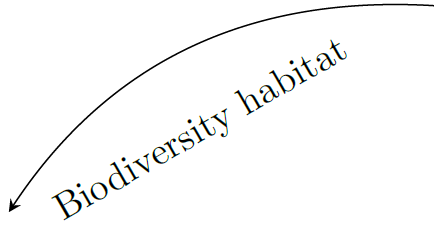
\includegraphics[width = 0.18\textwidth]{figures/wildland/arrow_biod.PNG}
    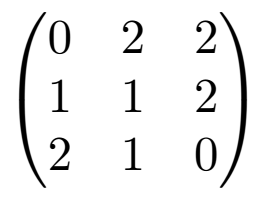
\includegraphics[width = 0.18\textwidth]{figures/wildland/land3.PNG}
    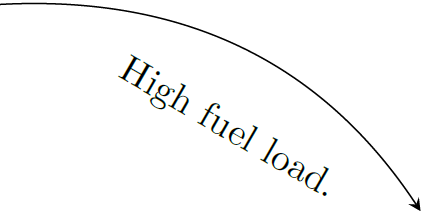
\includegraphics[width = 0.18\textwidth]{figures/wildland/arrow_fuel.PNG}
    \\
    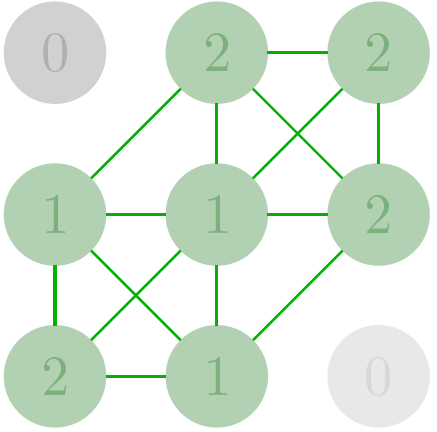
\includegraphics[width=0.2\textwidth]{figures/wildland/biodiv_3.PNG} \hspace*{4cm}
    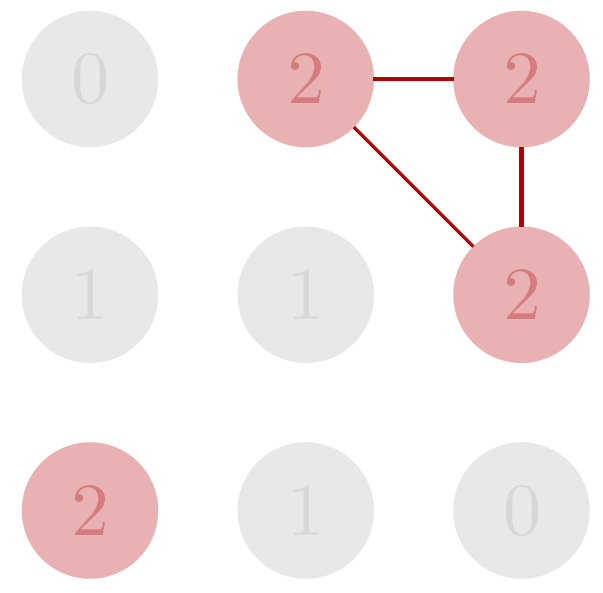
\includegraphics[width=0.2\textwidth]{figures/wildland/fire_3.PNG}\\
    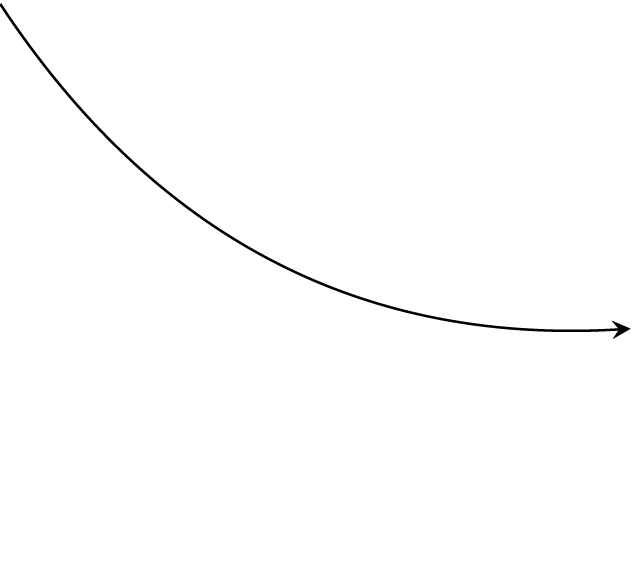
\includegraphics[width=0.18\textwidth]{figures/wildland/arrow_right.PNG}
    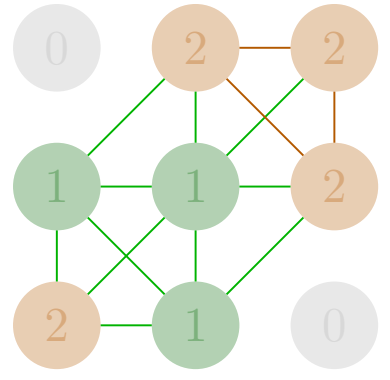
\includegraphics[width = 0.2\textwidth]{figures/wildland/graphe_feu_biod_33.PNG}
 	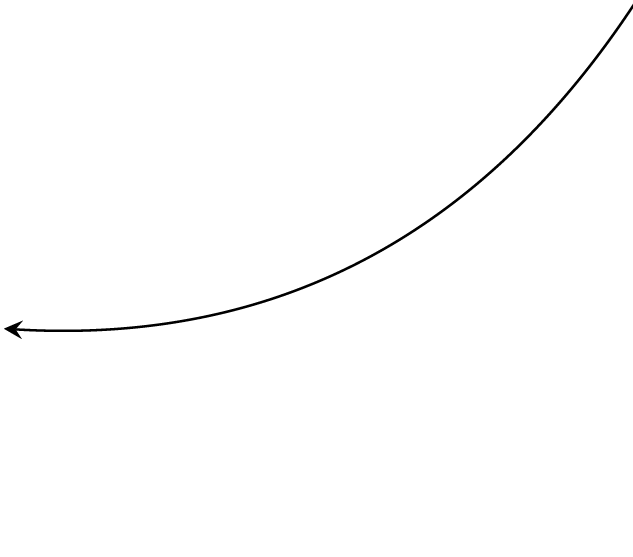
\includegraphics[width=0.18\textwidth]{figures/wildland/back_left.PNG}
    \caption{Illustration of the habitat and fuel graphs for $n=3$}
    \subcaption*{\hspace*{0.5cm}In this graph, green cells support biodiversity habitat only, while red cells display high risk. 
\\
    \hspace*{0.5cm}The high risk graph has two components (top right corner with 3 nodes, and bottom left corner with 1 node), while the biodiversity habitat graph only has one.
\\
    \hspace*{0.5cm}Cells for which the value is 0 are not considered as nodes for both graphs, and are thus not connected to the rest of the graphs. In the end, because high fuel load cells also support biodiversity habitat, the landscape can be represented as the overlap between the two graphs, where orange cells are high fuel load and also support biodiversity habitat.}

    \label{fig:graph_overlap}
\end{figure}

\newpage
\begin{figure}[H]
    \centering
    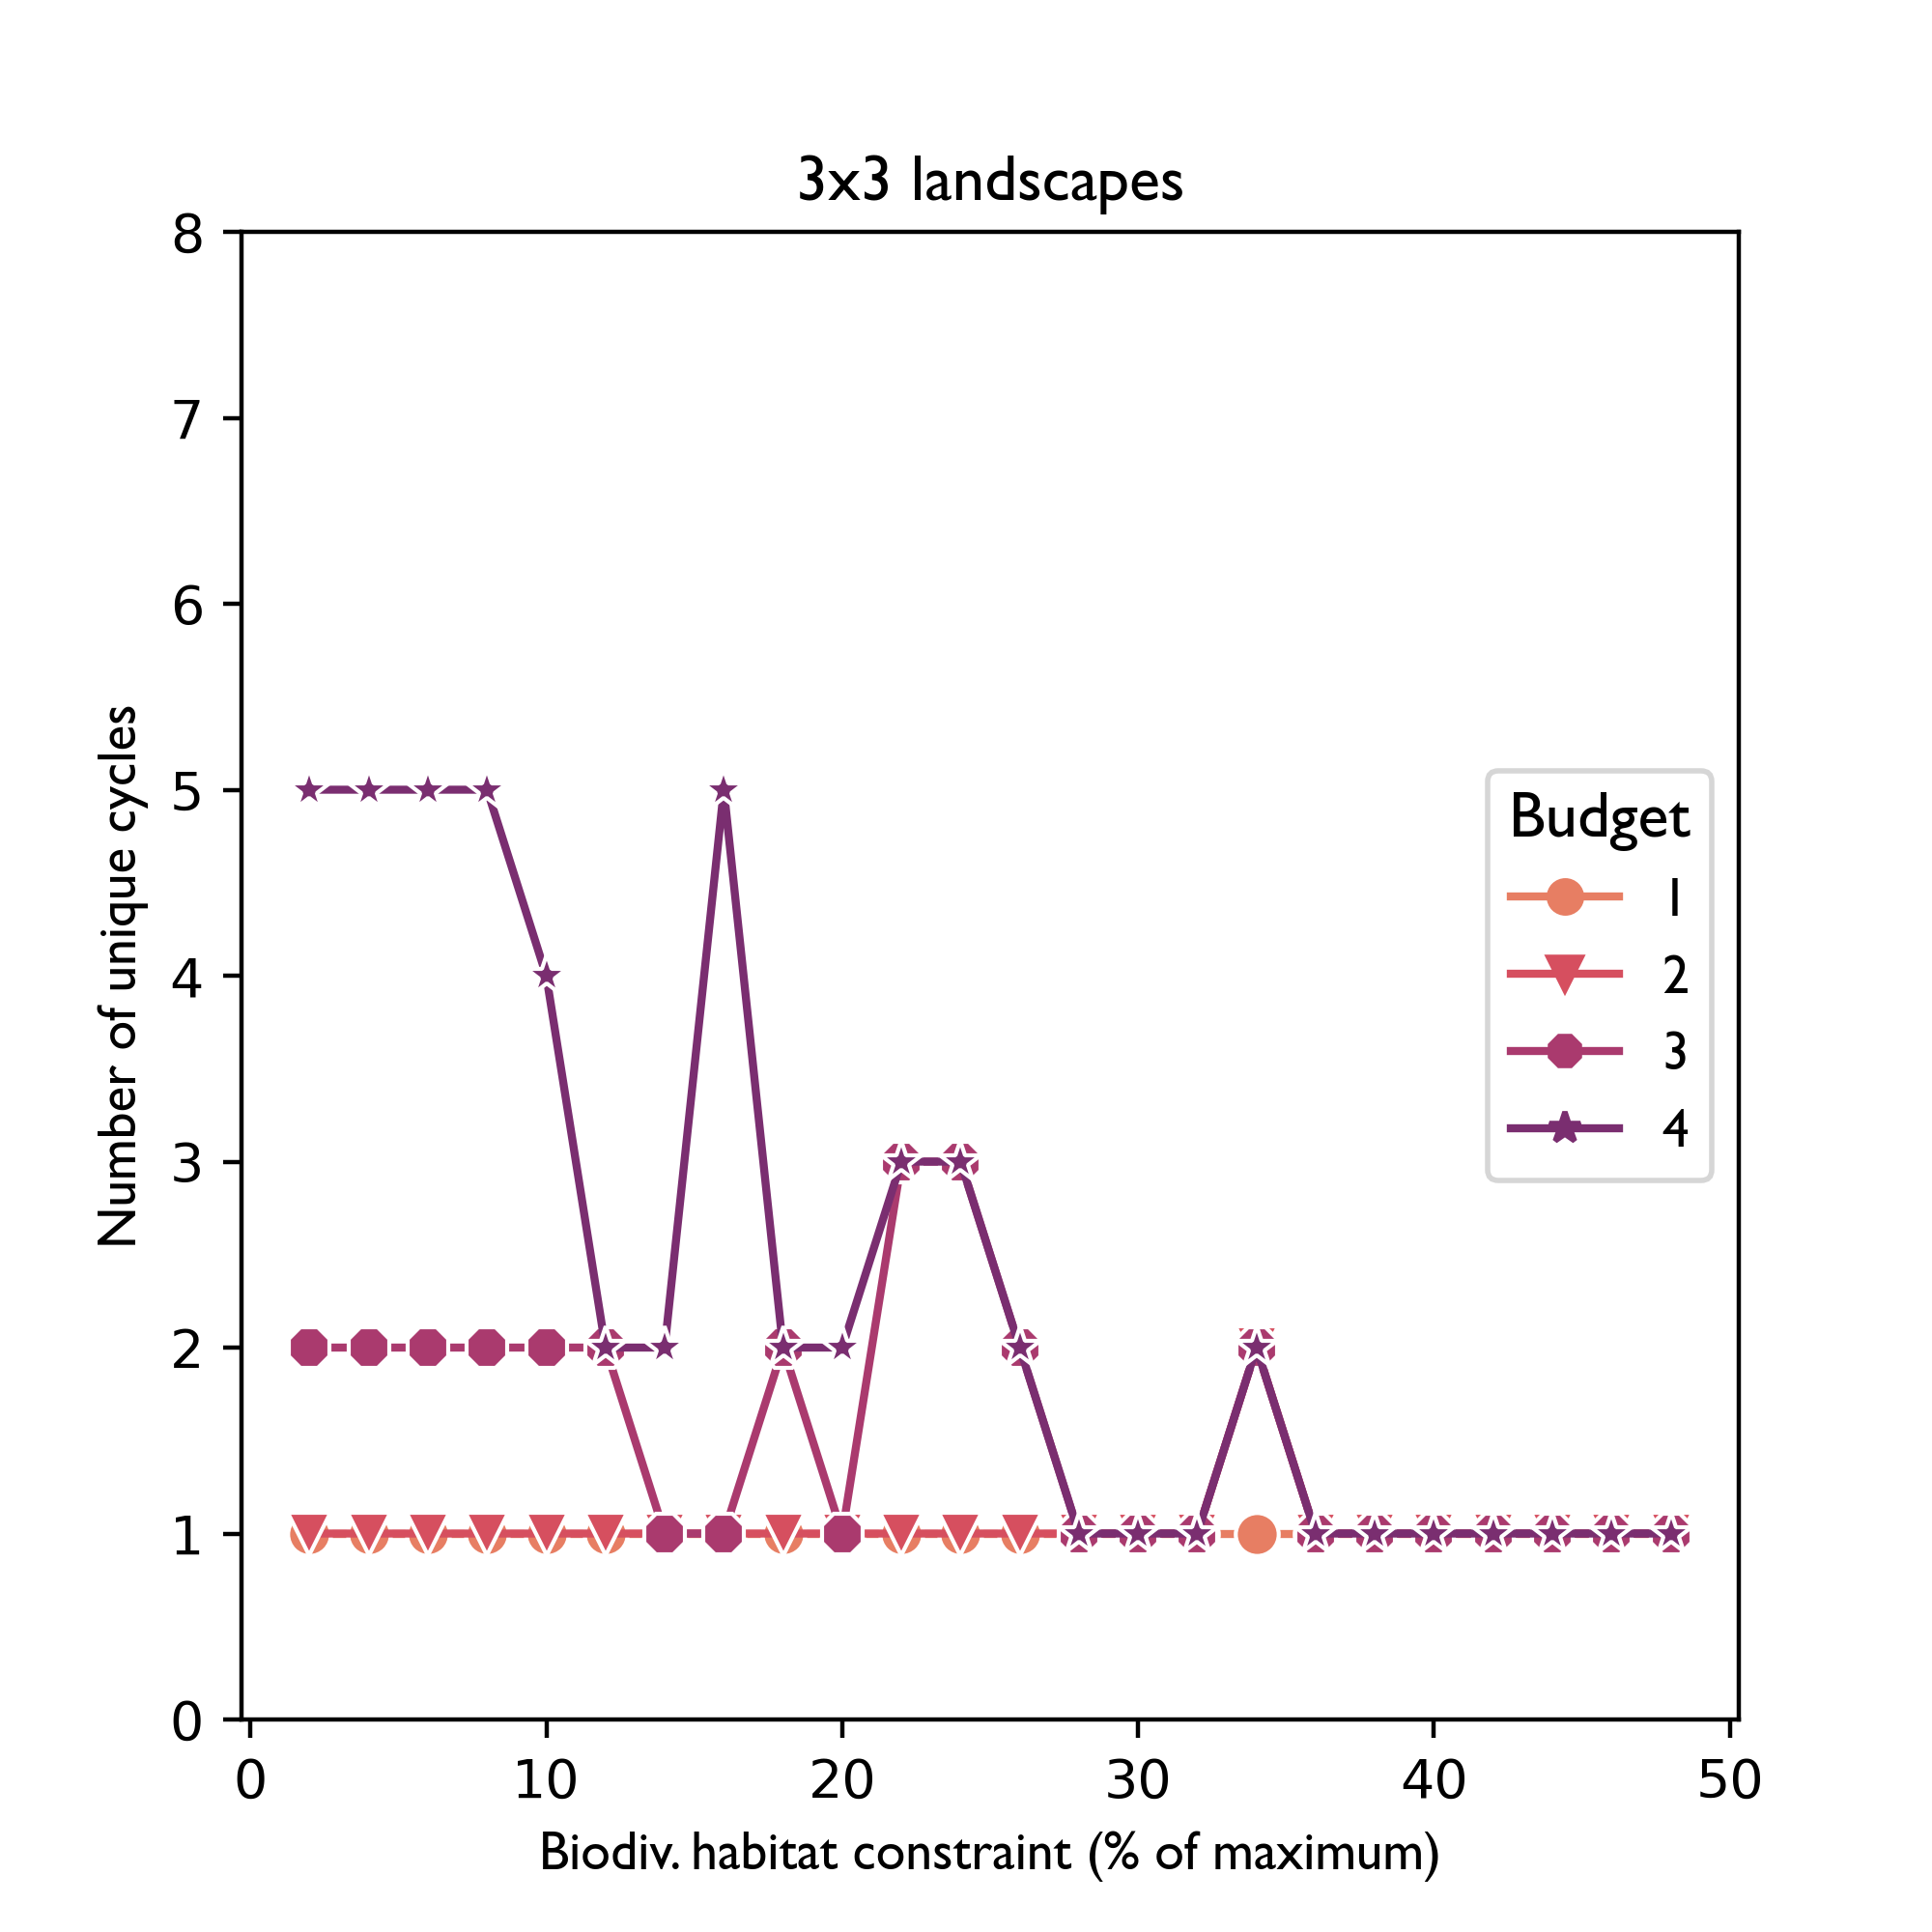
\includegraphics[width = 0.45\textwidth]{figures/wildland/number_cycles3.png}
    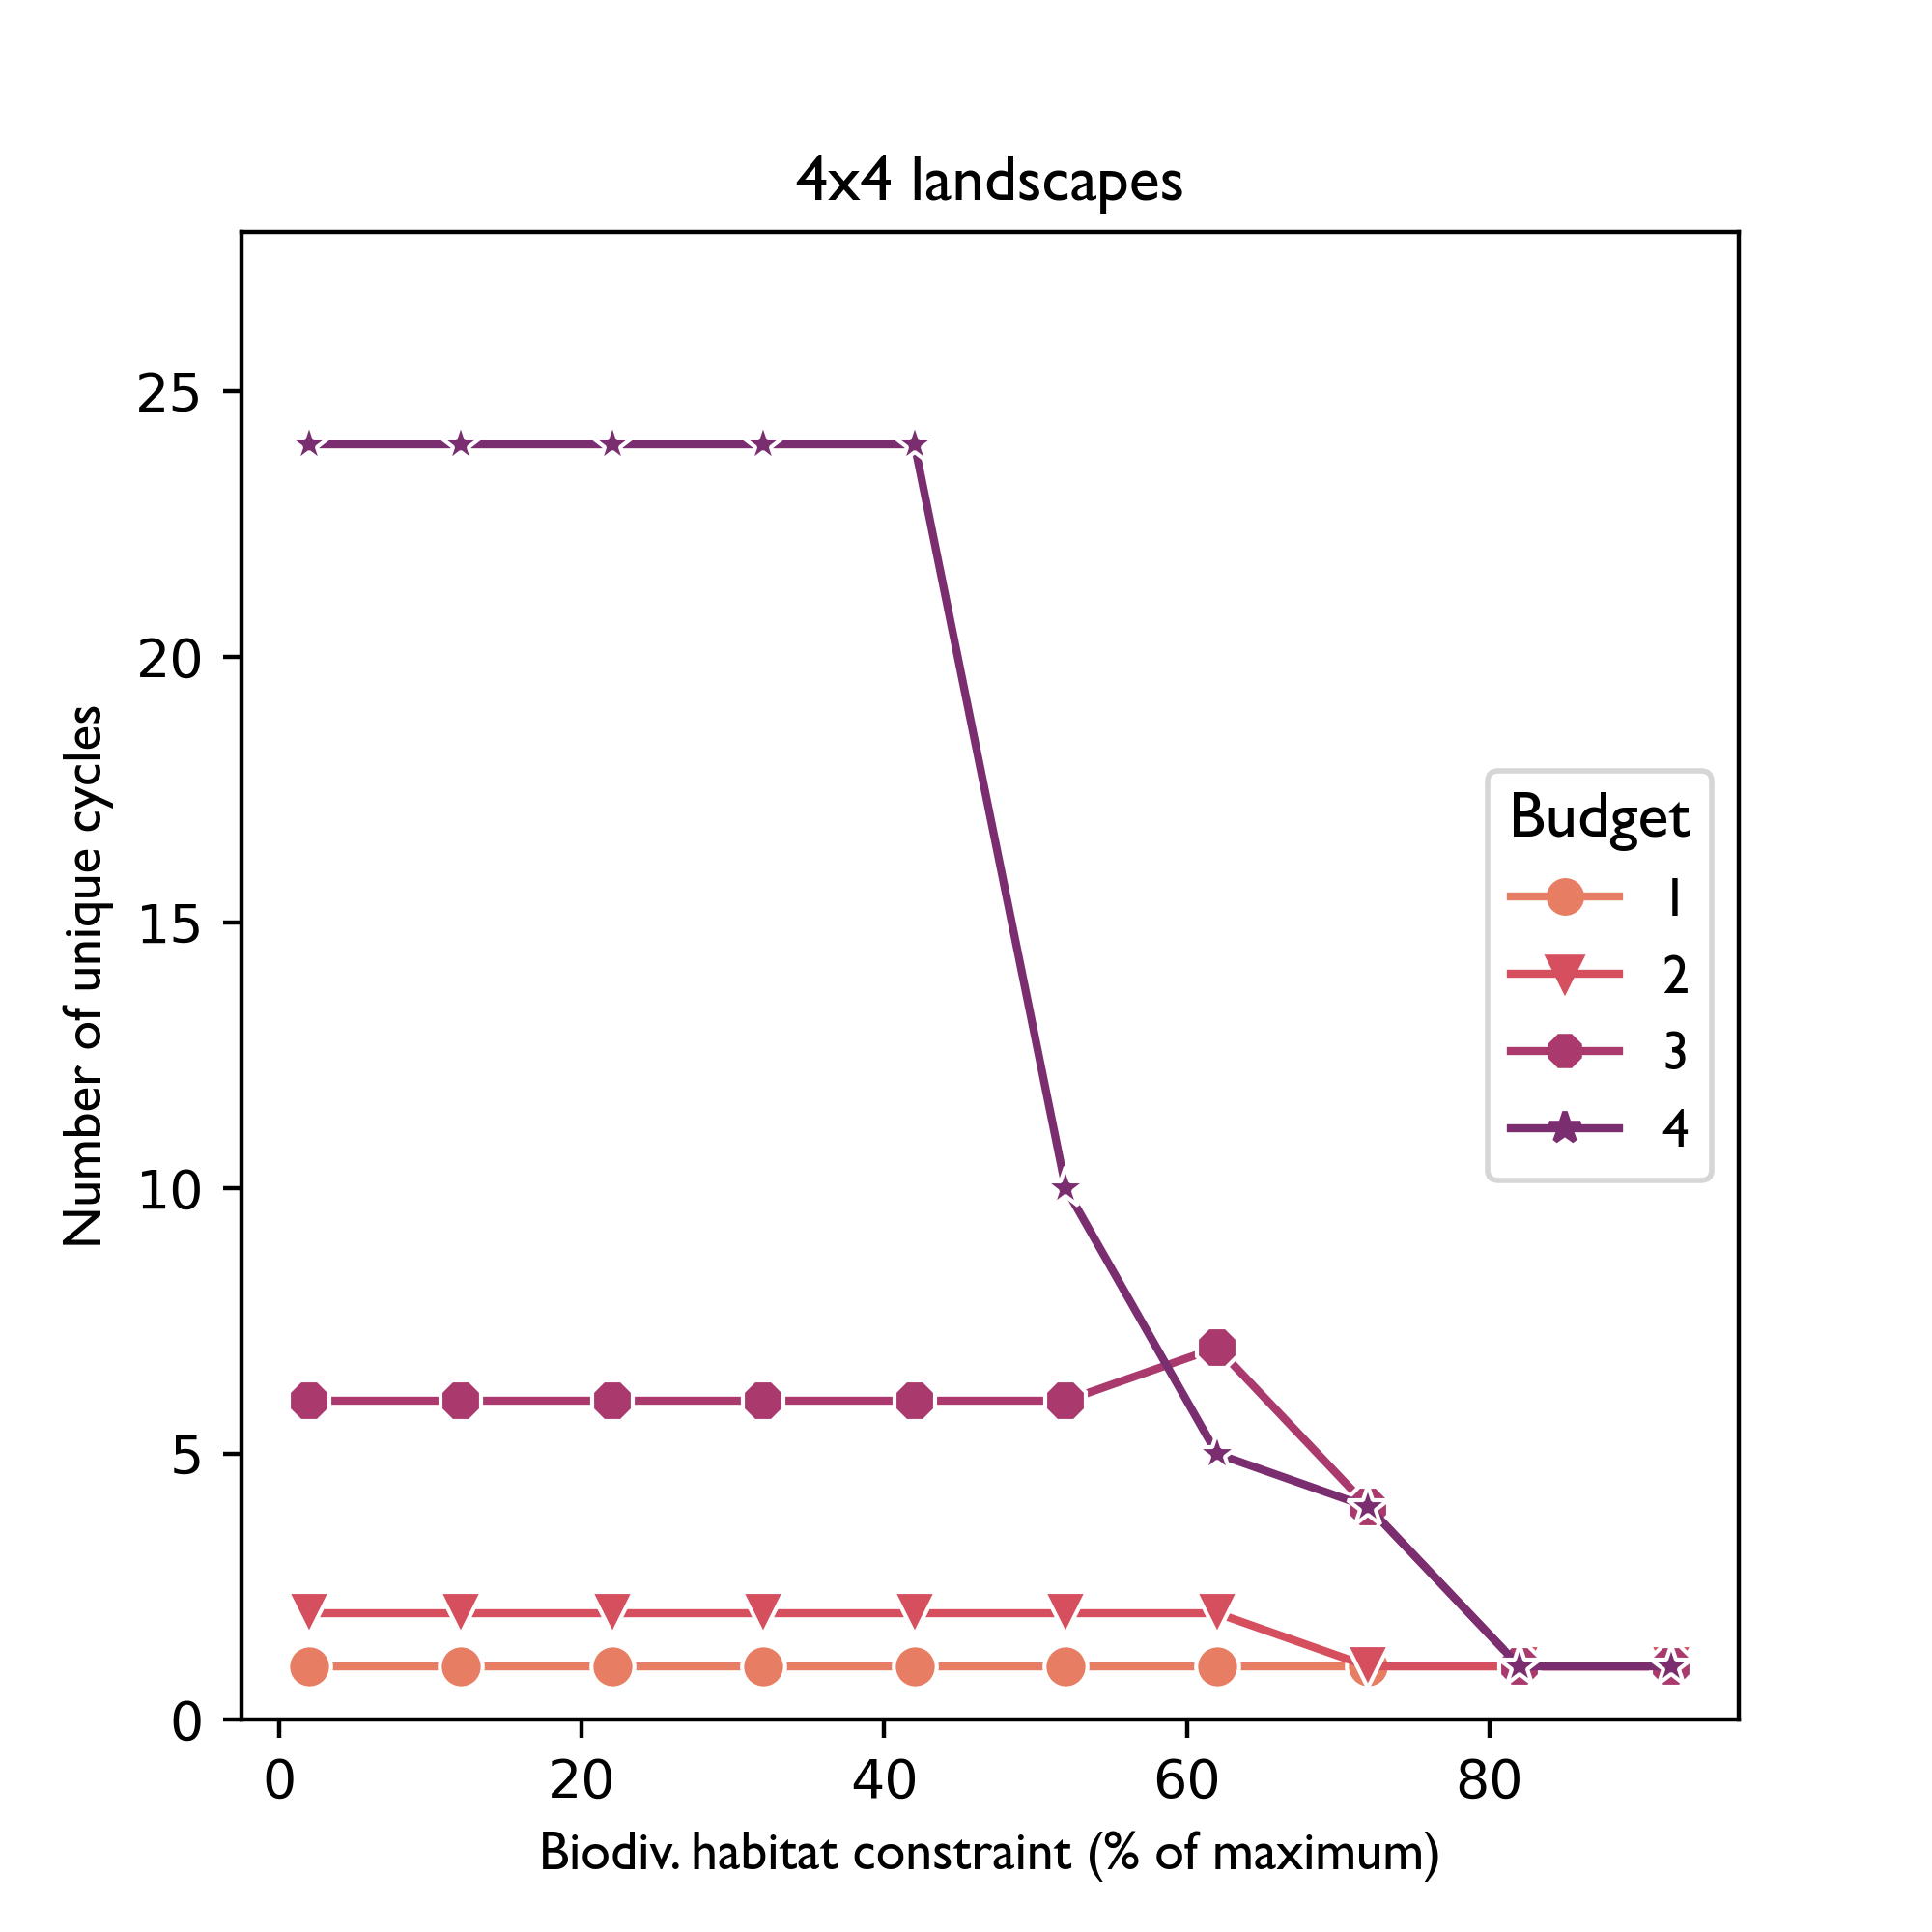
\includegraphics[width = 0.45\textwidth]{figures/wildland/number_cycles4.png}
    \caption{Number of cycles as a function of biodiversity habitat and budget}
    \label{fig:distrib_cycles}
\end{figure}
\newpage
\begin{figure}[h]
    \centering
    \includegraphics[width=0.5\textwidth]{figures/wildland/tradeoff3.png}\hfill
    \includegraphics[width=0.5\textwidth]{figures/wildland/tradeoff4.png}
    \\[\smallskipamount]
    \caption{Production possibility frontier between constraint (as a \% of maximum biodiversity sustainable in landscape) and wildfire risk for various budgets, and landscape size}
    \label{fig:frontier}
\end{figure}
\newpage

% Landscapes 
\begin{figure}[H]
    \centering
    \includegraphics[width=0.40\textwidth, height=9cm]{figures/wildland/landscapes3.png}
    \includegraphics[width=0.45\textwidth, height=10cm]{figures/wildland/landscapes4.png}
    \caption{Most represented cycles for each biodiversity constraint level, for various budget and landscapes $3 \times 3$, and $4\times 4$ (95\% CI shaded)}
    \label{fig:cycles_3_4}
\end{figure}
\newpage

\begin{figure}[H]
     \centering
     \begin{subfigure}[b]{0.4\textwidth}
         \centering
         \includegraphics[width=.98\textwidth]{figures/wildland/risky_surface3.png}
         \caption{}
         \label{fig:indicator_surface3}
     \end{subfigure}
     \begin{subfigure}[b]{0.4\textwidth}
         \centering
         \includegraphics[width=\textwidth]{figures/wildland/risky_surface4.png}
         \caption{}
         \label{fig:indicator_surface4}
     \end{subfigure}
     \hfill
     \begin{subfigure}[b]{0.4\textwidth}
         \centering
         \includegraphics[width=\textwidth]{figures/wildland/risky_components3.png}
         \caption{}
         \label{fig:indicator_component3}
     \end{subfigure}
     \begin{subfigure}[b]{0.4\textwidth}
         \centering
         \includegraphics[width=.98\textwidth]{figures/wildland/risky_component4.png}
         \caption{}
         \label{fig:indicator_component4}
     \end{subfigure}
     \hfill
          \begin{subfigure}[b]{0.4\textwidth}
         \centering
         \includegraphics[width=.98\textwidth]{figures/wildland/max_component_area3.png}
         \caption{}
         \label{fig:indicator_component3}
     \end{subfigure}
     \begin{subfigure}[b]{0.4\textwidth}
         \centering
         \includegraphics[width=\textwidth]{figures/wildland/max_component_area4.png}
         \caption{}
         \label{fig:indicator_component4}
     \end{subfigure}
        \caption{Assessment: surface, components of high-risk graph (95\% CI shaded)}
        \label{fig:indicators_1}
\end{figure}
\newpage

%\begin{figure}[H]
%    \centering
%    \includegraphics[width=0.45\textwidth]{squelette_draft/graphs_manuscript/risky_surface3.png} 
%    \includegraphics[width=0.45\textwidth]{squelette_draft/graphs_manuscript/risky_surface4.png}\\
%    \includegraphics[width=0.45\textwidth]{squelette_draft/graphs_manuscript/risky_components3.png}
%    \includegraphics[width=0.45\textwidth]{squelette_draft/graphs_manuscript/risky_component4.png}\\
%    \includegraphics[width=0.45\textwidth]{squelette_draft/graphs_manuscript/max_component_area3.png} 
%    \includegraphics[width=0.45\textwidth]{squelette_draft/graphs_manuscript/max_component_area4.png} 
%    \caption{Assessment indicators: surface and components of high-risk graph}
%    \label{fig:indicators_1}
%\end{figure}

\begin{figure}[H]
     \centering
     \begin{subfigure}[b]{0.4\textwidth}
         \centering
         \includegraphics[width=\textwidth]{figures/wildland/simpson_index3.png}
         \caption{}
         \label{fig:indicator_simpson3}
     \end{subfigure}
    \begin{subfigure}[b]{0.4\textwidth}
         \centering
         \includegraphics[width=.985\textwidth]{figures/wildland/simpson_index4.png}
         \caption{}
         \label{fig:indicator_simpson4}
    \end{subfigure}
    \hfill
     \begin{subfigure}[b]{0.4\textwidth}
         \centering
         \includegraphics[width=\textwidth]{figures/wildland/LSI_biod3.png}
         \caption{}
         \label{fig:indicator_LSI3}
     \end{subfigure}
     \begin{subfigure}[b]{0.4\textwidth}
         \centering
         \includegraphics[width=.985\textwidth]{figures/wildland/LSI_biod4.png}
         \caption{}
         \label{fig:indicator_LSI4}
     \end{subfigure}    
    \hfill
    \begin{subfigure}[b]{0.4\textwidth}
         \centering
         \includegraphics[width=\textwidth]{figures/wildland/diversity_index3.png}
         \caption{}
         \label{fig:indicator_diversity3}
     \end{subfigure}
    \begin{subfigure}[b]{0.4\textwidth}
         \centering
         \includegraphics[width=0.955\textwidth]{figures/wildland/diversity_index4.png}
         \caption{}
         \label{fig:indicator_diversity4}
    \end{subfigure}
        \caption{Assessment: diversity (95\% CI shaded)}
        \label{fig:indicators_2}
\end{figure}
\newpage


% Treatments 
\begin{figure}[H]
     \centering
     \begin{subfigure}[b]{0.48\textwidth}
         \centering
         \includegraphics[width=\textwidth]{figures/wildland/number_treatments3.png}
         \caption{}
         \label{fig:treatments_number3}
     \end{subfigure}
    \begin{subfigure}[b]{0.48\textwidth}
         \centering
         \includegraphics[width=\textwidth]{figures/wildland/number_treatments4.png}
         \caption{}
         \label{fig:treatments_number4}
    \end{subfigure}
    \hfill
     \begin{subfigure}[b]{0.44\textwidth}
         \centering
         \includegraphics[width=\textwidth]{figures/wildland/treatments3.png}
         \caption{}
         \label{fig:treatments_pattern3}
     \end{subfigure}
     \begin{subfigure}[b]{0.44\textwidth}
         \centering
         \includegraphics[width=\textwidth]{figures/wildland/treatments4.png}
         \caption{}
         \label{fig:treatments_pattern4}
     \end{subfigure}    
        \caption{Treatment allocation : number, location}
        \label{fig:treatments}
\end{figure}
%	\end{appendices}	
	

%%%%%%%%%%%%%%%%%%%%%%%%%%%%%%%%%%%%%%%%%%%%%%%%%%%%%%%%%%%%%%%%%%%%
%%%%%%%%%%%%%%%%%%%%%% CHAPTER FENCES %%%%%%%%%%%%%%%%%%%%%%%%%%%%%%
%%%%%%%%%%%%%%%%%%%%%%%%%%%%%%%%%%%%%%%%%%%%%%%%%%%%%%%%%%%%%%%%%%%%
	\renewcommand{\thesection}{\arabic{section}}
	\renewcommand{\thesubsection}{\arabic{subsection}}
	\setcounter{figure}{0}
	\setcounter{equation}{0}
	\counterwithout{figure}{section}
	\counterwithout{table}{section}
	\renewcommand{\thefigure}{3.\arabic{figure}}
	\renewcommand{\thetable}{3.\arabic{table}}	
	\renewcommand{\theequation}{3.\arabic{equation}}

	\chapter{Fences - The economics of connectivity in spatial renewable resources}
%\footnote{I am grateful to Lauriane Mouysset and Christopher Costello, Martin Quaas, Giorgio Fabbri, Francesco Ricci, Valentin Cocco, Jérôme Pivard, Lucas Vivier, Romain Fillon, Alexandre Adrian (from Platt Vineyard),  as well as seminar participants at BINGO, the 2024 FAERE PhD Workshop, 2024 Parisian PhD Seminar in Environmental Economics for their helpful comments.}}
\interfootnotelinepenalty=100

%To fragment or thin : 


\begin{minipage}{0.9\textwidth}
\singlespace
%This article discusses the complex interplay between ecological conservation and economic activities within spatially distributed networks. Renewable ressources, such as game, and invasive species on land can be managed through their stock, and landscape connectivity. This article examines how overharvesting (or under in the case of an invasive species) and habitat fragmentation can be jointly managed. Spatial connectivity can be managed to solve the tragedy of the commons and lead to efficient harvest as property rights are secured. Nonetheless, fragmenting habitat can be detrimental, and a trade-off emerges between efficient harvesting and optimal fencing. This article examines the optimal management of spatially distributed, endogenously connected renewables. In a setting where economic and biological conditions are heterogeneous and positively correlated, efficient management leverages a spatial arbitrage opportunity, promotes habitat connectivity, and optimizes welfare. With negative correlations, efficient management implies not changing what Nature has done, and harvest rules need to be enforced for welfare maximization. On the other hand, I look at the dynamic game that emerges when players can choose their harvest level and how their land connects to others. I show, under mild conditions, that the non-cooperative equilibrium results in fragmented habitat but halts overexploitation. In some cases, it can result in optimal management, depending on the underlying heterogeneous economic and biological conditions. Moreover, observed ecosystem dynamics can be partly rationalized through economic factors. For instance, observed sink-source dynamics may reflect heterogeneous biological productivities, and environmental features, but also heterogeneous returns to species in non-cooperative equilibria. 
%Finally, I  examine which policies should be implemented in a second-best framing, where connectivity or harvesting policies can be implemented, and rank policy options across heterogenous landscapes. 
%This article contributes to the literature on optimal renewable management and brings the fishery literature back on land, as connectivity can be managed. It contributes to the dynamic network formation games literature in the context of a renewable resource. I emphasize the need for policies that consider the interconnectedness of ecological systems and the different margins of economic activities that impact them, aiming for sustainable management practices that ensure both ecological integrity and economic viability.
%It explores how optimal resource management changes with endogenous connectivity. Moreover, as connectivity can be changed, the extent of spatial externalities can be limited. This article highlights conditions where solving the spatial externality is the first best scenario instead of leveraging what Nature has rightfully done. 

This article examines the management of spatially distributed renewable resources—specifically wildlife and infectious diseases—through the lens of economic and spatial analysis. I focus on "bads" like invasive species and diseases, which cause economic and ecological harm, and utilize population control and fencing as central  mechanisms. I analyze how fencing influences resource flow and connectivity. On the one hand, in the presence of ecological and economic heterogeneities, fencing can be used to leverage spatial artbitrage opportunities. On the other hand, while promoted as a tool to incentivize the internalization of costs associated with ``bads", they may undo what Nature has rightfully done. In this sense, while fencing may be welfare improving in a setting with initially poor connectivity, an uncoordinated use of fencing, although welfare improving, is not welfare maximizing. The study develops a theoretical model that integrates aspects of stock and patch connectivity management and explores both cooperative and non-cooperative management strategies. The findings indicate that optimal management often requires a nuanced understanding of the spatial dynamics and economic costs associated with different control strategies. We present a series of propositions that characterize the conditions under which fencing and resource control strategies can be optimized, including the interaction effects of exclusionary and trap effects. This article contributes to the literature by highlighting the role of spatial heterogeneity in the management of renewable resources and providing insights into the formulation of more effective environmental policies, as it analyzes how to design policies on a subset of the landscape, to maximize economic and ecological benefits. \\\\
\textit{JEL codes :} Q20, Q24, R12\\
\textbf{Keywords :} spatial resource management, invasive species; fencing and control strategies; optimal management; non-cooperative equilibrium; second-best policy.
\end{minipage}

\clearpage
\onehalfspacing
\section{Introduction}
% Motivation paragraph
%In the 1600s, the Ma'ohi,  the Indigenous People of the Society Islands in French Polynesia \citep{oliver2019} built vast fish traps, using organic fences, stakes, and poles. On the island of Huahine, stones set vertically, forming V-shaped enclosures trapped schools of fish coming down to sea, from a shallow salt water lake. Fish were pulled towards the sea with the tides, and became trapped in basins. Fish were then harvested using nets in the shallow lake. Managing the fish stock for the community amounted to more than harvesting.  Trapping, thus reducing the extent of fish school mobility, was instrumental\footnote{Modern applications, such as fish fences on Pacific islands, are detrimental to seascape connectivity, and destroy the sea bed, see \cite{exton_artisanal_2019}}.

In the Middle Ages in Europe, wildlife fencing primarily served to enclose aristocratic hunting reserves, such as deer parks or chases, where game like deer, boar, and rabbits were kept for the elite. These enclosures, often protected by wooden or stone barriers called \textit{pales}, not only preserved game but also safeguarded nearby farmland from wildlife incursions. However, these enclosures contributed to social tensions, as peasants were prohibited from hunting within them, and wandering game often damaged crops. A notable example is the \href{https://www.nationaltrust.org.uk/visit/hampshire/new-forest-northern-commons/the-history-of-the-new-forest}{New Forest} in England, established by William the Conqueror in 1079, where fencing symbolized the legal and social privileges of the nobility \citep{rackham_history_1987}. 

Centuries later in the US, populations of white tailed deers have skyrocketted to an estimated 36 million, with exceptionally high densities in the South East \citep{hanberry_regaining_2020}. At high densities, deer populations threaten the regeneration of forests as they influence species composition and abundance through browsing, hence damaging people's properties \citep{hanberry_does_2019}. Moreover, risks of zoonosis and epidemics increase with large populations. While large scale culling policies have been implemented, landowners have increasingly resorted to other methods, such as repellents, or fencing. Eight-foot or higher woven-wire fences have been used to protect agricultural land such as orchards or vineyards as well as private homes, to limit the damage done by growing deer populations \citep{caslick_economic_1979}.

Eventually, during the COVID 19 pandemic between 2019 and 2023, international airports and ports were shutdown, and extensive lockdown policies were implemented worldwide. By avoiding contact between infected and non-infected people, these policies aimed at slowing the spread of the pandemic\footnote{In a given population, where succesive infections are possible, lockdown policies aim at diminishing the basic reproduction number $\mathcal{R}_0$, which measure ``expected number of infections generated by a single and (typical) infected individual during their entire infection period'' see \cite{saldana_modeling_2022} for a primer SIR modeling applied to COVID 19}, while managing the extent of the economic losses associated with frozen national and international economies. 

These three examples display cases of management of spatially distributed renewable biological entity, species or virus, a renewable resource, either good or bad in time. Indeed, deer populations and pandemics grow through time, depending on the size of the population and location specific characteristics. Moreover, they move through land, jurisdictions and countries. These examples highlight that the management of spatially distributed renewable resources, whether goods or bads, involves at least two layers : managing the population, and how it moves through space. Indeed, culling and hunting deer population, and curing patients act as population management measures, repellents and fences keep the deers away (or within) and lockdowns avoid virus spread from infected to non infected people. Finally, in all cases, policies aimed at managing the movement of the resource are more efficient in one way than the other : wildlife exclusion fencing often have doors to let animals escape, and to a certain extent, people were prohibited from entering a country more than leaving one during the COVID 19 pandemic. 

These examples highlight the necessity to encompass both population and connectivity management when analyzing spatially distributed renewable resources, as they raise a number of challenges. 
First, the decentralized management of spatially distributed renewable resources is made difficult by the spatial externality they generate. Deer are an example of species whose status depend on people's preferences and assets. When communities compete for mobile deer, they anticipate part of the herd to migrate to other communities, and tend to overharvest, as they do not have secure property right over the whole resource through time \citep{kaffine_unitization_2010}. When deer are bads, free riding on neighbor's culling may deters people to cull the population to efficient levels \citep{costello_private_2017}. In this sense, patch connectivity, in a non cooperative setting, generates inefficiencies. As a consequence, fences appear as welfare improving, as they diminish patch connectivity and therefore contribute to solving the spatial externality. If a deer herd no longer migrates, communities would tend to harvest it in a more sustainable way. If on a given property, deer have no chance of re-entering, then one may undertake efficient culling measures. However, from a welfare perspective, fencing may undo what nature has rightfully done. Considering spatial heterogeneity in marginal returns to harvesting or culling, and biological productivity, a resource may flow naturally flow to where it is best managed. In this case, although fencing can solve the spatial externality and promote efficient resource use, it would not maximize welfare. Second,  spatially distributed renewable resources live on intricate institutional maps, between private and public land and sea. As a result, optimal harvesting and fencing may be difficult to decentralize. Hence, figuring the second best policy mix to best manage spatially distributed renewables is a challenge. \\
In this article, I focus on the management of ``bads", e.g. species that cause economic damages. This includes rodents, feral pigs, deer, or predators in areas where native species prey are threatened. I develop a theoretical model \textit{à la }\cite{costello_private_2017}, to understand the interplay between stock and patch connectivity management. Species are controled, grow and disperse through space, according to immutable environmental factors and expenditures that change connectivity, e.g. fences. Fences have two effects : they keep the bad out (\textit{exclusionary} effect), and they keep the bad in (\textit{trap} effect). In what follows, I assume the exclusionary effect dominates the trap effect. In most cases, exclusionary fencing keeps predators, or damaging species out, while allowing entrapped animals to leave the area\footnote{This can be viewed as an ecological version of inward and outward multilateral resistance terms \citep{anderson_gravity_2003}}. I analyze how the changes in local fencing patterns have local and spillover effects, and can be seen as changing multilateral resistance terms in an ecological context, and show how they affect each patch, under various management regimes. 
This approach can be viewed as an application of the spatial trade literature to ecological networks. For example, \cite{donaldson_railroads_2016} shows that railroads have a global effect, as they change the ``market access" of each county, accounting that local changes in ``market access" have spillover effects onto other counties. More generally, to understand the general equilibrium effect of domestic policies on international trade patterns, the use of a structural gravity model is inevitable (e.g. `the new quantitative trade model' e.g. \cite{arkolakis_new_2012}). However, the gravity equation fails at identifying the impact of country specific determinants of trade flows, e.g. multilateral resistance terms \citep{anderson_gravity_2003}.
% Case study with bads and deers
% The second best problem in a world with public land and private land

My contributions in this article are several. First, I characterize the value of dispersal in settings with exogenous dispersal. I outline the conditions under which connectivity changes the value of managing a spatially distributed public bad. In doing so, I outline the opportunity to consider the management of connectivity as a policy option to minimize aggregate damage, and that unless prohibitively costly, it is likely that decentralized decisions affect connectivity patterns.
Second, I study the optimal policy mix between stock and dispersal rate management. When costs of control are heterogeneous, the sole owner leverages the spatial arbitrage opportunity, and when fences only have an exclusionary effect, the sole owner redirects the population stock to where it's controled at the cheapest cost. In doing so, she reduces the population in more expensive patches further than when connectivity cannot be managed. Allowing for resource redispatch, she controls more of the species. When fencing has both an exclusionary and trap effect, cost heterogeneity does not suffice to redirect the resource. If biological productivity is larger in relatively costlier patches, trapping them can increase the aggregate cost of the invasive species. Therefore, depending on the structure of dispersal and how fencing affects it, fencing occurs when biological productivities and control costs are inversely correlated. 

Second, I characterize the non cooperative equilibrium in harvesting and fencing. When fencing only displays an exclusionary effect, and fencing is costless, every patch owner fences to the maximum. In doing so, they isolate their patch from the rest of the landscape, and control as if they were isolated from other patches. While this results in a more efficient level of control than in the case of uncontrolled spatial dependence, this is not welfare maximizing : as a matter of fact, the non cooperative equilibrium, while solving the spatial externality, does not leverage the spatial arbitrage opportunity provided by heterogenous costs of controling and biological productivities. When fencing displays (unequal) exclusionary and trap effects, best response functions are non monotonous. In this case, increasing fencing is not always optimal, and the Nash equilibrium results in suboptimal fencing, although closer to the optimal solution.



\section{Related literature}
\label{sec:related_literature}

There is a vast literature that investigates the optimal control, eradication and detection of invasive species (see \cite{epanchin-niell_economics_2017} for a review of the economics of prevention, detection and control of invasive species through space). A much scarcer one looks at the spatial nature of the management of public bads and/or invasive species. These literature can be classified into 3 strands : trade, economic epidomiology and resource economics with different types of approaches to connectivity, space, and population dynamics. 

Approaches from the trade literature consider the trade policy tools to avoid the introduction of alien invasive species. For example, \cite{olson_dynamic_2010} study the optimal use of sanitary and phytosanitary standards to prevent the introduction of pests through international trade. As pest and disease grow and spread over time their introduction has to be prevented. In a dynamic model, with non linear costs of trade restrictions, they investigate when full protection is efficient, and how prevention and control efforts need to be balanced. 

The economic epidemiology literature uses different versions of the Susceptible Infected Recovered model \citep{sir_model}, where the evolution of each subpopulation forms a system of ordinary differential equations depending on epidemiological parameters, such as the infection or recovery rate. Such models have been refined to encompass more compartments of the subpopulation, including spatial approaches (for the spread of crop disease using a mean-field approximation, see \citep{forster_optimizing_2007}), or age groups to guide policy during the COVID 19 pandemic \citep{gollier2020cost, acemoglu_optimal_2021}. In these models, different rates of spread among subpopulations are possible and can be accomplished with differentiated lockdown policies. Notably,  \cite{fenichel_economic_2013} studies the impact of social distancing and the impact of undifferentiated policies and include an endogenous component to the transmission rate, dependent on age specific characteristics and utility maximizing behavior, thus paving the way to analyze the endogeneity of disease spread and the role of economic incentives.

In the invasive species literature, early approaches such as \cite{huffaker_optimal_1992}, \cite{bhat_controlling_1996} analyze various management regimes (cooperative, isolated, and coordinated) to deal with the presence of beavers on private land. Using a framework stemming from metapopulation theory, they describe movement as a density dependent process, where relative densities dictate migration (an adaptation of Fick's Law of diffusion), which is, funny enough, an adaptation of Stenseth's ``\textit{social fence}'' hypothesis \cite{stenseth_social_1988}. Optimal stock management needs to account for the migratory effects associated with population levels. With this analysis, \cite{huffaker_optimal_1992} and \cite{bhat_controlling_1996} limit themselves to two patches, for analytical and computational tractability. In this framework, fences are not really described, although dispersal is an endogenous process. A different approach, viewing space as a continuum, has considered options to halt the progression of an invasive species, using barreer zones, to ultimately slow the rate of spread \cite{sharov_bioeconomics_1998}. While theoretically appealing, this approach may not be suited for operational concerns, whereby optimization on a continuum space is difficult, especially in various directions. \\
In the wake of \cite{brown_metapopulation_1997}, \cite{bulte_metapopulation_1999}, \cite{sanchirico_bioeconomics_1999} numerous models with spatially explicit metapopulation dynamics have been introduced, and soon became applied to the management of spatially distributed pests. For example, \cite{blackwood_cost-effective_2010} develop a linear quadratic framework to study the control of an invasive plant species. Taking advantage of the stock independent nature of dispersion patterns and of the linear quadratic structure, the authors solve the control and prevention problem at a large spatial scale. In more recent work, \cite{costello_private_2017} develop a large scale model of public bads, characterized by exogenous dispersal, stock-independent, and analyze the potential for eradication in a connected landscape. In doing so, they analyze the effects of varying connectivity parameters, without acknowledging for the potentially endogenous nature of dispersal. A  wealth of papers, in the wake of \cite{sanchirico_bioeconomics_1999}, several papers \citep{albers_invasive_2010, ambec_regulation_2012} have investigated the use of policies to halt the spread of invasive species, including mandatory refuges, albeit uniform. While these articles view dispersal as a characteristic that can be influenced, they do not consider the optimal management, or lack thereof, of dispersal. Several article acknowledge the endgeneity of dispersal, such as \cite{janmaat_sharing_2005}, who highlights the role of dispersal in a fishery, and other parameters, to assess the extent of the tragedy of the commons. Interestingly, in that article, Janmaat states that `` \textit{until ‘fences’ are available to contain the ‘wandering’ offspring, management zones would have to be large. This would minimize the spillover, bringing the incentives of the ‘owner’ into line with maximizing the total returngenerated by the resource}". \cite{horan_wildlife_2008} study conservation payments for various risk reducing ecological investments can be used to affect wildlife conservation and disease risk. In this article, they study how payments for ecosystem services affect habitat provision and connectivity for the Andean deer, to protect them from disease carried by livestock. The analysis focuses on the temporal dynamics of the number of patches in different ecological states, adopting an SIR-like structure (i.e. share of states occupied by susceptible livestock or wildlife etc) from \cite{mccallum_disease_2002}. The article does not study geographic, spatial patterns of habitat provision, but studies the provision of habitat in depth, and acknowledges the endogenous nature of habitat connectivity. In a more recent article, \cite{Wilen2012} study the optimal management of an invasive species on a gridded landscape where species dispersal follows a cellular automaton : habitat patches are either occupied or not, and spread can be stopped using containment. The main idea of the present article resembles the approach in \cite{Wilen2012}, but explicitly considers the dynamics of species, and extends the approach to non cooperative setings. Finally, \cite{bode_interior_2013} study the optimal use of interior fences (e.g. fraction the landscape into disconnected, equally sized patches) to reduce the costs of control of an invasive alien species on an island. While this approach is similar to the one developed in this article, it does not feature explicit spatial dynamics and ecological networks. 
In the current article, I build on these frameworks by using a discretized, raster-type landscape, with metapopulation dispersal across patches. Instead of analyzing how policies should adapt to dispersal, and I analyze how policies can shape dispersal and the decentralized, non cooperative equilibrium resulting from control and fencing decisions. 

%\begin{itemize}
%\item Burnett, 2008
%\item Costello and Quérou 2017
%\item Bhat and Huffaker 1996 - Controlling transboundary wildlife damage: modeling under alternative management scenarios

%\item Epanchin Niell \& Wilen 
%\item Blackwood et al 2010
%\item Broadly speaking, the literature on network games provides interesting insights highlighting that players’ behaviors
%are influenced by those around them (Jackson and Zenou, 2014)
%\item Olson and Roy, 2002
%\item Janmaat + check de la base
%\item Managing Urban Deer, Rondeau
%\item Gender-Based Harvesting in Wildlife Disease Management
%\item Jointly determined ecological-economic tradeoffs in wildlife disease management 
%\item Optimal harvesting of a plant-herbivore system : lichen and reindeer in Finland
%\item A note on the economics of bioinvasions
%\item An age-structured bio-economic model of invasive species management: insights and strategies for optimal control
%\item Invasive species management in a spatially heterogeneous world : effects of uniform policies
%\item Spatial management of Wildlife Disease
%\item Bioeconomics of managing the spread of exotic pest species with barrier zones
%\item Spatial Management of Invasive Species: Pathways and Policy Options
%\item Optimizing spatial and dynamic population based  control strategies for invading forest pests
%\item On Prevention and Control of an Uncertain Biological Invasion
%\item THE ECONOMICS OF CONTROLLING A STOCHASTIC BIOLOGICAL INVASION
%\item Metapopulation dynamics and stochastic bioeconomic modeling
%\item The economics of managing infectious wildlife disease 
%\item Bioeconomic management of invasive vector-borne diseases
%\item OPTIMAL TRAPPING STRATEGIES FOR DIFFUSING NUISANCE-BEAVER POPULATIONS
%\item Optimizing the Use of Barrier Zones to Slow the Spread of Gypsy Moth (Lepidoptera: Lymantriidae) in North America
%\item Application of distributed parameter control in wildlife damage management
%\item Optimal Control of Vaccine Distribution in a Rabies metapopulation model
%\item Pest as a common property resource : a case study of alfalfa weevil control
%\item Pests: Sustained Harvest versus Eradication
%\item Spatial Dynamics of Optimal Management in Bioeconomic Systems
%\end{itemize}


%Coordination of action through stock management but also maybe with fences etc. 

\section{A dynamic spatial model of renewable bads management : fencing and controlling}
\label{sec:model}

This model is adapted from \cite{costello_private_2017}. It conserves the main features and includes an endogenous determination of landscape connectivity. For this version, I simplify the set-up to two players to investigate the value of connectivity.  

\subsection{Spatial ecology}
Assume $2$ patches indexed $i\in \{A, B\}$ with a renewable resource. In a given period, the resource stock $X_{it}$ is controled by an amount $h_{it}$, and grows according to the remaining stock (or escapement), defined as $e_{it} = X_{it} - h_{it}$, such that the pre-dispersion population in patch $i$ in $t+1$ is $g_i(e_{it})$ such that $g(0)=0$, $g_i'(e_{it})\geq0, g_i''(e_{it}) \leq 0$, allowing for local extinction and recolonization. Moreover, after the resource grows, it disperses through space (see fig. \ref{fig:timing} for a summary of the model timing). This is consistent with metapopulation models \citep{sanchirico_bioeconomics_1999, bulte_metapopulation_1999}, although in a discretized timeframe \citep{costello_private_2017}. For now, I  assume that dispersal depends exclusively on exogenous, immutable environmental characteristics. Density effects on dispersal rates are not considered in this model, to disentangle the effect of control decisions from fencing decisions on optimal management. Following \cite{costello_private_2017}, dispersal rates from patch $i$ to $j$ is given by $d_{ij} \in [0,1]$. As we study a closed system, when the resource does not disperse, it remains in patch $i$ such that $d_{ii} = 1 - d_{ij}$. Therefore, in each period, a flow $d_{ij}g_i(e_{it})$ leaves patch $i$ \textbf{to} patch $j$ and a flow $d_{ji}g_j(e_{jt})$ leaves \textbf{from} patch $j$ to patch $i$. \\
In conclusion, the patch specific population dynamics are given by : 
\begin{align}
X_{it+1} &=  d_{ji} g_j(e_{jt}) + \left(1 - d_{ij}\right)g_i(e_{it}) \nonumber \\
& = g_i(e_{it}) + \left( d_{ji} g_j(e_{jt}) - d_{ij} g_i(e_{it}) \right)
\end{align}

The first term denotes the population growth in patch $i$, and the second term in parenthesis denotes the net immigration from patch $j$ to patch $i$. In terms of notations, $\mathbf{D}$ refers to the matrix of dispersal rates.

\subsection{Spatial economy}

The presence of bads is costly in each patch via two channels, modeled as in \cite{costello_private_2017}. First, the presence of bads implies property specific control expenditures. The larger the population, the lower the marginal cost of control: controling the first unit at large population levels is cheaper than when the population is small. Marginal control costs feature a stock effect, where the marginal cost of control $c_i(s)$ is decreasing with stock size, $c'_i(s)<0$. The total cost of controlling down to residual stock $e_{it}$ is $\int_{e_{it}}^{X_{it}}c_i(s)ds$. 

Additionally, the presence of the residual stock causes heterogeneous marginal damages (for example, deer cause more damages to orchards and managed forests  than to meadows) $k_i(s)$, which increase with stock size $k'_i(s)>0$, resulting in convex damages. The total damages caused by the residual stock is $\int_{0}^{e_{it}}k_i(s)ds$.

The total cost in each patch $i$ and period $t$ is : 

\begin{equation}
C_i(e_{it}, X_{it}) = \int_{e_{it}}^{X_{it}}c_i(s)ds + \int_{0}^{e_{it}}k_i(s)ds
\end{equation}

The patch-period specific cost depends on current patch specific decisions, as well as past decisions by other agents, which influence the stock of bad in patch $i$ at the beginning of period $t$. Finally, for ease of notation, variables in bold font are in vector form, e.g. $\mathbf{X}_t = (X_{At}, X_{Bt})$.

\section{The value of connectivity}

In this section, I first illustrate the value of changing connectivity patterns, and how fences can change them. To do so, I solve for the social planner of the model following \citep{costello_private_2017} and illustrate how the value function changes with connectivity parameters. 

\subsection{Optimal residual stock in a connected world without fences}
Before introducing the optimal determination of $f_{At}$ and $f_{Bt}$, I focus on the case where $f_{At} = f_{Bt} = 0$, to illustrate the effects of changing the connectivity patterns \textit{ex-nihilo}.  Following \cite{costello_private_2017}, the social planner aims to minimize the aggregate intertemporal welfare in patches $A$ and $B$. Her program is : 
\begin{align}
\min_{\{\mathbf{e}_t\}_{t=0}^\infty}& \sum_{t=0}^\infty \delta^t \left(\sum_i C_i(e_{it}, X_{it}) \right) \nonumber  \\
\forall i& \in \{A, B\}: \nonumber  \\\
& X_{it+1} = g_i(e_{it}) + (d_{ji}g_j(e_{jt} - d_{ij}g_i(e_{it}))
\end{align}

The Bellman equation can be written as:

\begin{align}
V(\mathbf{X}_t) & = \min_{\mathbf{e}_t} \left( \sum_i C_i(e_{it}, X_{it}) + \delta V(\mathbf{X}_{t+1}) \right) \nonumber  \\
& = \min_{\mathbf{e}_t} \left( \sum_i C_i(e_{it}, X_{it})\right. + \nonumber \\
 &\delta V\large( g_{A}(e_{At}) + (d_{BA}g_B(e_{Bt}) - d_{AB}g_A(e_{At});\nonumber \\
& \left. g_{B}(e_{Bt}) + (d_{AB}g_A(e_{At}) - d_{BA}g_B(e_{Bt})\large)\right)
\end{align}

Following proposition 5 of \cite{costello_private_2017}, the optimal residual stock is given by :
\begin{proposition}
The sole owner optimal control strategy has residual stocks $\bar{\mathbf{e}}_{t}>0$ characterized as follows : 
\begin{equation}
k_i(e^*_{it}) = c_i(e^*_{it}) - \delta \sum_jc_j(x_{jt+1})d_{ij}g'(e^*_{it})
\label{eq:foc_costello}
\end{equation}
As long as $k_i(0)  - (1 - \delta (1 - d_{ij}g_i'(0))c_i(0) + \delta g'_i(0) d_{ij} c_j(0)<0$, otherwise $e^*_{it}=0$. 
\label{proposition:interior_costello}
\end{proposition}

As shown in \cite{costello_private_2017}, this defines a state-independent solution, where $\bar{\mathbf{e}}_t$ does not depend on $\mathbf{X}_t$ (a version of the proof is given in appendix). For an interior solution, the current marginal damage must equal the marginal cost of control, net of the future costs of control imposed by controling one more unit of the bad. However, if the marginal damages are sufficiently low, or the dynamic costs expected to rise sharply, then the optimal solution is eradication. As such, in a disconnected world, local eradication and interior solutions can coexist. 

A key question is to what extent are optimal residual stocks changing with given connectivity patterns. Optimal residual stock adapts to changes in dispersal in non trivial ways. As the social planner aims at keeping dynamic marginal costs balanced across patches, she has to change her optimal residual stocks when dispersal changes to account for differences in marginal costs. 
First, consider a world with homogeneous marginal control costs (i.e. where the difference only comes from the stock level, but costs are identical for a given population level) and growth. Consider any level of dispersal from $B$ to $A$ and low levels of dispersal from $A$ to $B$.  An increase in dispersal from $A$ to $B$ mechanically reduces the population in the next period in $A$, thus giving room to control more and lower residual stock in $A$, to reduce the aggregate costs. This is possible as the population level remains substantial, thus keeping the marginal cost of control relatively low. For example, if 5\% of a deer herd migrates to a neighboring patch (and 95\% remains), the additional 1\% dispersion allows to control more, as damages are reduced, and the size of the herd is still substantial enough, such that it is not difficult to cull the population by one more unit. 
\\
At larger levels of dispersal from $A$ to $B$, an increase in dispersal has a different effect. As the level of pest is already low, the marginal control cost of the remaining units is large. Hence, while the dispersal lowers the future population, and potentially its cost, maintaining a given level of residual stock comes at a very expensive cost. To continue with the deer example, if dispersal increases from 90\% to 95\%, continuing to cull the population at the same level becomes very expensive, as it is difficult to find the remaining individuals. Hence, residual stock is reduced, to use the low marginal level cost and variation in $B$ and avoid an overburden in $A$.\\

Second, consider the effect of a marginal increase in inward dispersion (i.e. change in $d_{BA}$). At low levels of outward dispersion (e.g. $d_{AB} = .1$), the population in $A$ is already large. Any increase in the future population level in $A$ comes at a substantial cost, and to maintain equal costs across the landscape, the social planner sends some of the bad back by reducing residual stock in $A$. Now, at larger levels of outward dispersal (e.g. $d_{AB} = .7$), the same mechanism applies for low increases in ingoing dispersal $d_{AB}$. However, the response changes, as here, more pest flow from $A$ to $B$. In doing so, the cost in $B$ is increased : to reduce the aggregate cost, residual stock in $A$ must decrease. Proposition \ref{prop:escapement_variation} establishes these effects. 
\begin{proposition}
\label{prop:escapement_variation}
In the case where optimal residual stock is interior (i.e. $\forall i e^*_{it}>0$) :
\begin{itemize}
\item $\frac{\partial e_{it}}{\partial d_{ij}}$ is non monotonous (decreasing and increasing)
\item $\frac{\partial e_{it}}{\partial d_{ji}}$ can be non-monotonous, and when monotonous, can be increasing or decreasing depending on the level of $d_{ji}$
\end{itemize}
\end{proposition}
Finally, these effect depend on the fact that different stocks have different costs. With heterogeneous linear marginal costs, residual stock react in a monotonous way to changes in dispersal to balance the change in aggregate costs. With homogeneous non-linear marginal costs, different levels of population cause different control costs, even though they are on the same curve. Absent some sort of heterogeneity, there is no change in optimal residual stock, as the dynamic marginal control costs are equal across patches, and heterogeneous levels may only arise from differences in marginal damages and growth patterns across patches
%\footnote{Indeed, with homogeneous linear marginal costs $c$, eq. \ref{eq:foc_costello} can be rewritten as : 
%\begin{equation}
%c - k_i(e_{it}) = c\delta g_i'(e_{it})
%\end{equation}
%The optimal escapement thus defined is independent of dispersal parameters.}.\\
%
Finally, changes in connectivity patterns can break interior solutions and foster either eradication, or residual stock is limited by the stock and no control is undertaken (i.e. $e_{it}=X_{it}$). In this case, the optimal solution in proposition \ref{proposition:interior_costello} no longer holds and the optimal residual population depends on the population in $t$, $X_{it}$. In the case of source-sink dynamics, i.e. when patch $A$ retains a lot of the its population, while the population from patch $B$ leaves almost integrally to $A$, control is not undertaken in $B$ : the marginal cost of control is too important. More control is undertaken in $A$, and the aggregate stock decreases. 

\subsection{Analytical value of marginal dispersal changes}

The value function, in turn, can be rewritten taking into account the dispersal matrix $\mathbf{D}$ as : 

\begin{equation*}
V(\mathbf{X}_0, \mathbf{D}) = \sum_{i \in \{A,B\}}\left( \int_{0}^{e^*_{it}} k_i(s) ds + \int_{e^*_{it}}^{X_{it}} c_i(s)\right) + \delta V(X^*_{1})
\end{equation*}

Using this formulation, one can identify the effect of a change in connectivity. For example, the value of a change in connectivity (through a change in dispersal from $A$ to $B$, see Appendix ) : 
\begin{align}
\frac{\partial V(\mathbf{X}_0, \mathbf{D})}{\partial d_{AB}} = & g'_A(e_{At}^*)(c_B(X_{At+1}^*) - c_A(X_{Bt+1}^*)) + \nonumber \\
& \frac{\partial e_{At}^*}{\partial d_{AB}} \left(g_A'(e_{At}^*) (c_A(X_{At+1}^*)(1- d_{AB}) + d_{AB} c_B(X_{Bt+1}^*\right)+ \nonumber \\
& \frac{\partial e_{Bt}^*}{\partial d_{AB}}\left(g'_B(e_{Bt}) (c_A(X_{At+1}^*) d_{BA} + (1- d_{BA})c_B(X_{Bt+1}^*)\right) \label{eq:variation_of_value_function}
\end{align}
Welfare changes through direct and indirect effects of changes in dispersal patterns. The first line measures the direct effect of a change in dispersal from $A$ to $B$, as the stock grows in $A$ and travels from $A$ to $B$, thus incurring marginal control costs in $B$ rather than in $A$. The second and third lines measure the adaptation of the optimal residual stock to changes in dispersal. As highlighted above, the effect of a change in dispersal has ambiguous effects on optimal residual stock. The effect of a change in dispersal on welfare depends on how optimal residual stock change in both patches. The changes in optimal residual stock cause a change in growths in each patch. In patch $A$, the marginal unit of bad $g'A(e_{At}^*)$ remains for $(1-d_{AB})$\% in patch $A$ and causes control costs $c_A(X_{At+1}^*)$, while $d_{AB}$\% moves to $B$ and causes control costs $c_B(X_{Bt+1}^*)$ there. \\
Depending on the initial dispersal pattern $\mathbf{D}$, changes in connectivity patterns have intricate effects, as the reaction of optimal escapement is non-monotonous. Welfare changes with connectivity in the presence of heterogeneous, stock-dependent marginal costs of control, as spatial arbitrage opportunities exist. As the impact of marginal changes in connectivity patterns can be both positive and negative, optimal connectivity exists, depending on the nature of marginal damages, marginal costs and growth. 
Using these variations, one can compute the global effect of a change in connectivity patterns. However, this is beyond analytical tractability. Hence, I move onto a numerical illustration. 

\subsection{Numerical illustration}

I specify the problem using functional forms to illustrate the value of connectivity. Table \ref{table:functions_and_parameters} lists the functional forms as well as the associated parameterization. I use a linear quadratic damage function, an inverse marginal cost function, and a logarithmic growth function, with calibrated parameters, to ensure the emergence of an interior solution. Figure \ref{fig:illustration_functions} illustrates these functions. 

\begin{table}[h!]
\centering
\begin{tabular}{|c|c|c|c|}
\hline
\textbf{Function} & \textbf{} & \textbf{$A$} & \textbf{$B$} \\ \hline
\multirow{2}{*}{Marginal Cost} & \multirow{2}{*}{$mc_i(x) = \frac{\gamma_i}{1+ k_ix_i}$} & $\gamma_A = 10$ & $\gamma_B = 10$ \\ 
 &  & $k_A = 4$ & $k_B = 4$ \\ \hline\hline
\multirow{3}{*}{Marginal Damage} & \multirow{3}{*}{$md_i(x) = md_0 + md_1 x_i^2$} & $md_{1A} = 2$ & $md_{1B} = 2$ \\ 
 &  & $md_{0A} = 2$ & $md_{0B} = 2$ \\ 
 &  &  &  \\ \hline\hline
\multirow{2}{*}{Growth Function} & \multirow{2}{*}{$g_i(x) = a_i \times \log(1+b_i x)$} & $a_A = 0.95$ & $a_B = 0.95$ \\ 
 &  & $b_A = 1$ & $b_B = 1$ \\ \hline\hline
\multirow{1}{*}{Initial Stock} & \multirow{1}{*}{} & $X_{A0} = 1$ & $X_{B0} = 1$ \\ \hline\hline
\multirow{1}{*}{Planning Parameters} & \multirow{1}{*}{} & $\delta = 0.95$ &  \\ 
\multirow{1}{*}{Planning Parameters} & \multirow{1}{*}{} & $T = 50$ & \\ \hline
\end{tabular}
\caption{Parameter Definitions for model illustration}
\label{table:functions_and_parameters}
\end{table}

Using the implicit solution defined in proposition \ref{proposition:interior_costello}, I solve the model over $T=50$ periods, using the full range of $d_{AB}$ and $d_{BA}$.

\subsubsection{Optimal residual stock and dispersal}

Figure \ref{fig:figure1} displays the optimal levels of residual stock and the subsequent population levels through time, across quartiles of the value function. Results are symmetric. For lower values of the value function, optimal residual stock is relatively low in both patches, and increases as the value function increases gradually. The spread between residual stocks narrows as dispersal parameters become more symmetric. The dispersal patterns allow for more control in the case of sink-source dynamics, thus lowering the value function. 

\begin{figure}[H]
        \centering
        \includegraphics[width=\textwidth]{figures/fences/escapement_Baseline.jpg}
        \caption{Optimal stock and residual stock levels across patches for quartiles of the value function}
        \label{fig:figure1}
\end{figure}

Figure \ref{fig:escapement_derivative_interior} shows the variations in residual stock for interior and corner solutions. For low values of dispersal from $A$ to $B$, residual stock in $A$ decreases, but increases after $d_{AB}>.5$. Variations depend on the relative magnitude of $d_{AB}$ and $d_{BA}$, and display the non linear trends highlighted in proposition \ref{prop:escapement_variation}. Finally, figure \ref{fig:escapement_derivative_overall} shows the evolution of optimal residual stock, constrained by low stock levels in respective patches. 


\subsubsection{Value and connectivity}

The mechanisms highlighted above are illustrated in the surface map of the value function across $d_{AB}$ and $d_{BA}$. For sink-source dynamics (top right and bottom left corners), the dispersal patterns allow to control more of the population, resulting in lower population through time and lower damages. As dispersal patterns are more symmetric, the optimal intertemporal costs tend to increase. Ultimately, although the numerical values only serve an illustrative purpose, they show a stark result: if connectivity is manageable at limited costs, leveraging spatial arbitrage opportunities can increase welfare by almost 40\%. 

\begin{figure}[H]
	\centering
	\includegraphics[width=.8\textwidth]{figures/fences/heat_map_values_Baseline.jpg}
	\caption{Intertemporal costs of mobile public bad depending on landscape connectivity patterns}
\end{figure}



\section{Introducing fences}
\subsection{Definition and properties}
\label{sec:subsection_fences_definition}
As there is value to manage connectivity, connectivity measures are likely being implemented, unless they are prohibitively costly. In this part of the model, dispersal rates between patches depends on directional fencing expenditures in both patches, with $d_{ijt+1} \equiv d_{ijt+1}(f_{it}, f_{it})$, where $f_{it}$ measures the amount of fencing in patch $i$ in direction of patch $j$, as a percentage rate of maximal fencing, such that $F=\{f_{it} + f_{it} \leq 2\}$.  The rate of inward dispersion of invasive species from $i$ to $j$, $d_{ijt+1}(f_{it},f_{it})$ decreases with $f_{jt}$. I call this the "exclusionary effect": fences keep nuisances out of $j$. When fencing in $i$ at $f_{it}$, the outward dispersion of invasive species from $i$ to $j$ decreases as well, as species get trapped in $i$. This effect is the "trap effect" : fences trap the nuisance in. However, in most cases of exclusionary fencing, the exclusionary effect dominates the trap effect, allowing for trapped animals to escape. Fencing reduces the inward dispersion from $i$ to $j$ at a decreasing rate, whether it is undertaken in patch $i$ or $j$. The rate of patch retention $d_{iit+1}$ is the remainder after dispersions from $i$ to $j$. When no fencing is undertaken, the dispersal rate remains at a rate determined by immutable environmental factors (landscape discontinuities, mountains, terrain ruggedness etc), such that $d_{ijt+1}(0,0) = m_{ij}$. When the maximal amount of fencing is undertaken, dispersal drops to $n_{ij}$. 
Dispersal rates are ultimately affected by immutable environmental factors (landscape discontinuities such as roads, rivers, moutains; altitude and terrain ruggedness etc).
\begin{equation}
\begin{aligned}
d_{ijt+1} : F \to [n_{ij},m_{ij}] \subset [0,1] \\
\underbrace{\frac{\partial d_{jit+1}}{\partial f_{it}}}_{\text{Exclusionary effect}} \leq \underbrace{\frac{\partial d_{ijt+1}}{\partial f_{it}}}_{\text{Trap effect}} \leq 0\\
 d_{ijt+1}(f_{it}, f_{it}) + d_{iit+1} =1
\end{aligned}
\label{eq:dispersal_with_fences}
\end{equation}
As such, fences have public good features: whether $A$ or $B$ fences, both the inbound and outbound dispersal are affected, while only pf them pays the price.

In practice, for numerical simulations, I adapt dispersal rates from metapopulation theory using a negative exponential dispersal kernel \citep{hanski_estimating_2000, MOILANEN2004533}. Fencing acts as increasing the distance between patches, and conversely, as reducing the mean dispersal distance of a species in a given patch : 
\begin{equation}
d_{ijt+1}(f_{it},f_{jt}) = \exp(-\theta( f_{jit} + \beta_i f_{ijt})\times (m_{ij} - n_{ij}) + n_{ij}
\end{equation}
Where $\theta$ is a scaling parameter, and $\beta_i$ measures the relative effect of fences in $i$ compared to fences in $j$ to reduce $d_{ijt+1}$. Figure \ref{fig:dispersal_illustration} illustrates dispersal between $A$ and $B$ with asymetric bounds to dispersal (i.e. $m_{ij} \neq m_{ji}$ and $n_{ij} \neq n_{ji}$). 

\begin{figure}[H]
	\centering
	\includegraphics[width=.6\textwidth]{figures/fences/illustration_dispersal.jpg}
	\caption{Dispersal depending on fencing decision in $A$ and $B$ with asymetric bounds and cross efficiencies}
	\subcaption*{On the left panel, $\beta_A=.8$ describes a situation where the trap effect dominates, while on the right panel, $\beta_A = 1.2$ displays a situation where the exclusionary effect dominates}
	\label{fig:dispersal_illustration}
\end{figure}

Fences change dispersal in a specific way, as they only diminish connectivity \textit{between} patches, and increase self retention. In the case where patches have the same bounds to dispersal ($n_{AB} = n_{BA}$ and $m_{AB} = m_{BA}$), fencing is not in the interest of the social planner : 
dispersal remains symmetric, and the value function does not vary along the symmetry axis between $d_{AB}$ and $d_{BA}$. Indeed, when fencing retains as much population in as it does keep out, the net effect on the next period population is null. As fences come to a certain cost, it always outweighs inexistant benefits. However, when bounds to dispersal are asymmetric, fencing can have a positive effect on welfare. As dispersal is decreased to asymetric inferior bounds, the population stock across patches changes asymetrically as well. In doing so, one can leverage the spatial arbitrage opportunity associated with asymetric dispersal and non-homogenous nonlinear costs, as well as different marginal damages. 


\begin{figure}[htbp]
    \centering
    \begin{subfigure}{0.45\textwidth}
        \centering
        \includegraphics[width=\textwidth]{figures/fences/heatmap_with_symmetric_dispersal_large.jpg}
        \caption{Inefficient changes in connectivity with symmetric natural bounds}
        \label{fig:figure1}
    \end{subfigure}
    \hfill
    \begin{subfigure}{0.45\textwidth}
        \centering
        \includegraphics[width=\textwidth]{figures/fences/heatmap_with_asymmetric_dispersal.jpg}
        \caption{Efficient changes in connectivity with asymmetric natural bounds}
        \label{fig:figure2}
    \end{subfigure}
    \caption{Efficient and inefficient changes in landscape connectivity}
    \label{fig:overall}
\end{figure}

\subsection{Spatial ecology and economy with fences}

With fences, the spatial ecology of the problem is modified as follows, with $d_{ijt+1}(f_{it}, f_{it})$ defined as in equation \ref{eq:dispersal_with_fences}: 

\begin{align}
X_{it+1} &=  d_{jit+1}(f_{it}, f_{it}) g_j(e_{jt}) + \left(1 - d_{ijt+1}(f_{it}, f_{it})\right)g_i(e_{it}) \nonumber \\
& = g_i(e_{it}) + \left( d_{jit+1}(f_{it}, f_{it}) g_j(e_{jt}) - d_{ij}(f_{it}, f_{it}) g_i(e_{it}) \right)
\end{align}

Fences are expressed as a percentage of the maximal rate of fencing doable. Anecodtal evidence suggests that fencing costs increase in a convex way: marginally reducing the passage of species or viruses can be done at a low costs, while more efficient devices can reach large costs\footnote{Methods range from scent and taste-based repellents, that need to be reapplied frequently and cost 15-50\$ per gallon, to electric fencing (at 3-5\$ a foot), and landscape modifications such as gullies and dams (ranging from 500 to 5,000\$ per work), and finally, regular human presence. In the case of viruses, strategies range from wearing surgical masks to partial and complete lockdowns, with different economic costs. \cite{gollier2020cost, acemoglu_optimal_2021} analyze the costs of different lockdown strategies with multigroup SIR models, in the context of COVID 19. They focus on age-specific disease spread rates, which is akin to considering spatially differentiated spread rates. They show that efficient, targeted lockdown strategies are paramount as their costs are convex.}. For the sake of simplicity, I nonetheless restrict the analysis to linear costs, such that the current payoff is modified. The total cost in each patch $i$ and period $t$ is : 
\begin{equation}
C_i(e_{it}, X_{it}, f_{it}^1, ..., f_{it}) = \int_{e_{it}}^{X_{it}}c_i(s)ds + \int_{0}^{e_{it}}k_i(s)ds  +  \kappa_i f_{it}
\end{equation}


















%\section{A spatially disconnected world}
%
%
%\subsection{Optimal fencing and controling}
%\label{sec:optimal_management}
%Assume a sole owner has to manage patches $1$ to $N$. She can decide how much to control in each patch, as well as to what degree patches are connected to minimize the total cost of the public bad, through time.  Her aim is to equalize the dynamic marginal costs of pest through space and time. 
%
%Her objective is to minimize the present value of aggregate costs across patches over time:
%
%\textbf{write the optimization program}
%
%The Bellman equation is :
%\begin{equation}
%V(X_{1t}, ..., X_{Nt}) = \min_{\forall i \{e_{it}, \{f_{it}\}_{j\neq i}\}} \sum_{i = 1}^N C_i(e_{it}, X_{it}, f_{it}^1, ..., f_{it}) + \delta V(X_{1-t+1}, ... X_{Nt+1})
%\label{eq:bellman}
%\end{equation}

%As a benchmark, we characterize the optimal control of the species in each patch, if each patch is isolated and dispersal cannot be managed (or at prohibitive costs) by the social planner (e.g.$\forall i,j$, $m_{ij}=n_{ij}=0$, thus $d_{ijt+1}(f_{it}, f_{it}) = 0$). As in \cite{costello_private_2017}, the first order conditions for an interior solution are : 

%\begin{proposition}
%\label{proposition:benchmark_no_space}
%If $\forall i,j$, $m_{ij}=n_{ij}=0$, then, $\forall i,j$ and $\forall t$ : 
%	\begin{align}
%		f_{it} &= 0\\
%	\end{align}
%	And : 
%	\begin{align}
%	\bar{e}_{it} > 0 &\iff k_i(\bar{e}_{it}) = c_i(\bar{e}_{it}) -  \delta g_i'(\bar{e}_{it})c_i(X_{it+1})\\
%	\bar{e}_{it} = 0 &\iff k_i(0) - c_i(0) \delta g_i'(0)c_i(0)>0
%		\label{eq:control_no_space}
%	\end{align}
%	
%\end{proposition}
%
%This result is expressed in \cite{costello_private_2017} in proposition 5 and 6. In a spatially disconnected world, the sole-owner controls the efficient amount in each patch. For an interior solution, the current marginal damage must equal the marginal cost of control, net of the future costs of control imposed by controling one more unit of the bad. However, if the marginal damages are sufficiently low, or the dynamic costs expected to rise sharply, then the optimal solution is eradication. As such, in a disconnected world, local eradication and interior solutions can coexist. Additionally, as connectivity cannot be managed, the marginal benefits of any fence are null, hence there is no fence. 
%Proposition \ref{proposition:benchmark_no_space} establishes that fact. 

%\subsection{Non cooperative equilibrium}

%\textbf{Establish the correspondence in the decentralized case. }
%In this case, each patch owner optimally controls the patch specific population, accounting for a dynamic stock effect : as the population is treated at a lower level, marginal growth is important and lowers the future cost of effort. 

\section{A world with endogenous connectivity and population}

\subsection{Socially optimal management: conditions for interior solutions}

When dispersal can be managed (i.e. $n_{AB}\neq m_{AB}$ and/or $n_{BA}\neq m_{AB}$), the sole owner decides both the levels of fencing and residual stock. Proposition \ref{proposition:optimal_sole_owner} establishes the conditions under which both interior fencing and residual stock exist:

\begin{proposition}
\label{proposition:optimal_sole_owner}
Interior optimal residual stock in each patch $i$ is such that : 
\begin{equation}
k_i(e_{it}) = c_i(e_{it}) - \delta g'_i(e_{it})\left[c_i(X_{it+1}) + d_{ijt+1}(f_{it}, f_{it})c_j(X_{jt+1}) - c_i(X_{it+1})) \right]
\label{eq:optimal_harvest}
\end{equation}

And optimal fencing in patch $i$ towards patch $j$ is : 
\begin{equation}
\kappa_i = \delta\left(\frac{\partial d_{ij+1}}{\partial f_{it}} g_i(e_{it}) - \frac{\partial d_{jit+1}}{\partial f_{it}}g_j(e_{jt})\right) \big(c_i(X_{it+1}) - c_j(X_{jt+1})\big)
\label{eq:optimal_fencing}
\end{equation}
Additionally, interior fencing and control are state-independent i.e. solutions do not depend on $\mathbf{X}_t$ (see proof in appendix \ref{appendix:proof_stock_independence_foc}).
\end{proposition}

 The optimal residual stock in patch $i$ is such that the current marginal damage caused by letting the marginal unit matches the corresponding control cost, mitigated by the discounted global cost effect, as in \cite{costello_private_2017} (refered to as the \textit{dynamic marginal cost effect}). When a marginal unit of bad is controlled, marginal damage $k_i(e_{it})$ are not incurred in patch $i$. This marginal damage has to equal the current period cost of controling $c_i(e_{it})$, and the discounted next period cost. A marginal unit of bad will grow according to $g_i'(e_{it})$, and disperse through space. A portion $d_{iit+1} = 1 - \sum_{j\neq i}d_{ijt+1}(f_{it}, f_{it})$ remains in the patch (and sets the marginal cost of control at $c_i(X_{it+1})$, while a fraction goes in each connected patch $j$, incurring a decrease in marginal control costs of $c_j(X_{jt+1})$. The extent of control thus depends on the current marginal damages and costs, and the spatial dynamic component. If dispersal to neighbors is \textit{naturally} large, and the marginal cost of control tends to be lower in these patches, residual stock increases, leveraging a spatial arbitrage opportunity.

Interior fencing is a novel result. In a given patch, the sole owner fences such that the current marginal cost of fencing equals the discounted marginal benefits of fencing. These benefits emerge from the use of a spatial arbitrage opportunity. Positive fencing occurs in $i$ if the \textit{exclusionary} effect of fencing (i.e. the marginal population that remains in $j$ following an increase in fencing in $i$) outweighs the \textit{trap} effect (i.e. the marginal population that remains in $i$ following an increase in fencing in $i$), and the marginal cost of control are larger in $i$ than in $j$. Positive fencing in $i$ can also emerge if the \textit{trap} effect dominates the \textit{exclusionary}, but control costs are larger in $j$ than in $i$. To further characterize the optimal management, I restrict the analysis to the case of constant marginal costs of control. In the next subsections, I disentangle the effects of the trap and exclusion effects with constant marginal costs of control.


\subsubsection{No fencing in the absence of spatial arbitrage opportunity}

The spatial arbitrage opportunity arises from the difference in control costs across space and for different stock levels. In that case, the absence of control cost heterogeneity implies no fencing : redirecting the resource flow has no interest, since there is no additional cost reduction to be expected. Although patches are connected, there is no heterogeneity to leverage. As a consequence, the optimal control rule is independent of dispersal. 
 In this case, the discounted future cost of controlling the increased stock in patch $i$ equal the current costs net of damages. Moreover, the optimal control does not depend on spatial dispersal, as the cost of control are homogenous, and depends only on patch specific characteristics. In this specific homogeneous linear case, the equilibrium collapses to the disconnected optimal control strategy defined in proposition \ref{proposition:homogeneous_cost}.

\begin{proposition}
\label{proposition:homogeneous_cost}
With linear homogeneous control costs (e.g. $\forall i$, $c_i(s) = c$), or no spatial dispersal (i.e. $d_{ii} = 0$ and $d_{jj}=0$), optimal management consists in no fencing $\forall i, j$, $f_{it} = 0$ and optimal residual stock is implicitly defined by:
$$
		c \delta g_i'(e_{it}) = c - k_i(e_{it}) 
$$
See proof in appendix \ref{appendix:proof_absence_fencing}
\end{proposition} 


\subsubsection{Optimal management with heterogeneous costs and exclusionary fencing}
\label{sec:optimal_exclusionary}

Assume control costs are heterogeneous, such that $c_A> c_B$. In this case, there is a potential to levy a spatial arbitrage opportunity : if the stock were more directed towards patch $B$, larger levels of control could be undertaken with the same budget (or equivalently, the same amount of aggregate control could be undertaken at a lower cost). 
In this example, I assume fencing only has an exclusionary effect. In real life, exclusionary fencing is a common practice in conservation. For example, the Kilauea Point National Wildlife Refuge in Hawaii has implemented a predator exclusion fence to protect native seebirds from mammalian predatiors\footnote{The 11,200 foot fence protects 168 hectares of wildlfe habitat and even includes underground skirt and curved hood to avoid climbing over or digging under, see \url{https://www.fws.gov/story/2023-08/pacifics-largest-predator-exclusion-fence}}. I focus on the case where exclusionary fences allow the population of predators to escape\footnote{In this case, the fencing technology can be seen as akin to an electrical resistance}.\\
In patch $A$, if fencing only has an \textit{exclusionary effect} and no \textit{trap} effect, fencing keeps the stock from $B$ out, while allowing the stock from $A$ to escape. Upon fencing, the sole owner gains clear marginal benefits, as the stock that used to flow from $B$ to $A$ no longer does, and the stock can still flow from $A$ to $B$, reducing the total cost. In this case,  the sole owner has an interest in reshaping how the stock moves through space, and thus, to reshape the spatial externality, such that resources flow to patch $B$.\\

\begin{proposition}
\label{prop:exclusion_optimal}
With heterogeneous, constant marginal cost of fencing such that $c_A>c_B$, $[n_{ij},m_{ij}] \subset ]0,1[$ and fencing only displays an exclusionary effect i.e. : 
\begin{align*}
& d_{ijt+1}(f_{it},f_{jt}) = d_{ijt+1}(f_{jt})\\
& \frac{\partial d_{ijt+1}}{\partial f_{jt}}<0
\end{align*}
The optimal allocation is : 

\begin{align}
\kappa_A &= \delta(c_A - c_B)\left|\frac{\partial d_{BAt+1}}{\partial f_{At}}(f_{At}^*, 0) \right|\\
f_{Bt}& = 0\\
k(e_{At}) &= c_A - \delta g_A'(e_{At})\large(c_A (1-d_{ABt+1}(0)) + c_B d_{ABt+1}(0))\large)\\
%
k(e_{Bt}) &= c_B - \delta g_B'(e_{Bt})\large(c_B (1-d_{BAt+1}(f_{At}^*)) + c_A d_{BAt+1}(f_{At}^*)\large)
\end{align}
\end{proposition}
Proposition \ref{prop:exclusion_optimal} shows that when spatial arbitrage opportunities are not exhaustable, the sole owner fences only in $A$ to avoid inward dispersal from $B$, while it does not change how much $B$ receives inward dispersion, as any dispersion from $A$ to $B$ is welfare improving. The response of optimal residual stock to changes in dispersal depends on the second order conditions of the problem\footnote{As a matter of fact : 
\begin{equation}
\frac{\partial e_{Bt}}{\partial f_{At}} = \frac{\kappa_A}{SOC_B}\delta g'(e_{it})
\end{equation}
Where $SOC_B = k_B'(e_{Bt}) + \delta g''_B(e_{Bt})((1 - d_{BAt+1}(f_{At}^*))c_{B} + d_{BAt+1}(f_{At}^*)c_A)$ is the second order condition of the problem with respect to $e_{Bt}$. As I do not fully analyze the second order conditions, it is impossible to substantiate claims further. However, notice that is negative when the increase in the marginal damage is lower than the increase in dynamic costs, and positive otherwise. As conditions for a global minimum differ with multivariate objective functions, this is a possibility to investigate further}.

%Eradication occurs in patch $A$ if 
%\begin{equation}
%k_A(0) - c_A + \delta g_A'(0)[(1-d_{ABt+1}(f_{At}^*,0)) c_A + d_{ABt+1}(f_{At}^*,0)c_B) >0
%\end{equation}
%And : 
%\begin{align*}
%\forall t>1, \text{ }e_{At} &= 0 \\
%k_B(e_{Bt}) &= c_B - \delta g_B'(e_{Bt})\large(c_B (1-d_{BAt+1}(0,f_{At}^*)) + c_A d_{BAt+1}(f_{At}^*,0)\large)
%\end{align*}
%Additionally, if fencing is free and connectivity can integrally be managed (i.e. $n_{ij} = 0$ and $m_{ij}=1$ $\forall i \in \{A, B\}$), damages are homogeneous ($k_A() = k_B() = k()$) then : 
%\begin{align*}
%f_{At} &= 1 \\
%f_{Bt} &= 0 \\
%\Rightarrow & d_{ABt+1} = 1 \text{ and } d_{BA} = 0\\
%\forall t>1, \text{ }e_{At} &= 0 \\
%k_B(e_{Bt}) &= c_B - \delta g_B'(e_{Bt})c_B
%\end{align*}
%\end{proposition}
%\subsubsection{Free fencing} 
Assume now that fencing only has a trap effect. For example, small scale fencing has long been used in the US to manage feral pigs populations, where animals get entrapped, but more can come in\footnote{see \url{https://www.aphis.usda.gov/sites/default/files/managing-feral-pigs.pdf}}. In patch $A$, if fencing only has a \textit{trap effect} and no \textit{exclusionary} effect, fences keep the stock inside of $A$, while they do not reduce the inward dispersion from patch $B$. As costs of control are smaller in $B$ than in $A$, a sole owner would benefit from keeping the population in $B$ where it is cheaper to control, and let the population from $A$ get trapped in $B$. The mechanism described here is \textit{in fine} symmetrical to the \textit{exclusionary} case, but fences are located in $B$.

%The sole owner can choose management to equate returns across space. When there is a spatial dependence, and connectivity is fixed by natural parameters, patches with high marginal costs of control, control less than in the no-dependence case. Symmetrically, patches with low marginal costs of control control less when they are not connected, as they can benefit from the dynamic marginal cost effect with population inflow from other patches. When the extent of connectivity can be managed (e.g. $n_{ij}>0$ and $0< m_{ij}\leq 1$), fencing arises in high control cost patches, and is kept at the minimal level in low control cost patches. In doing so, escapement decreases in high cost patches, and increases in low cost patches. 

%\begin{proposition}
%	If fences are free and only have an exclusionary effect, fences and control are substitutes
%	\\
%	see proof in appendix \ref{sec:appendix_proof7}.
%\end{proposition}


\subsubsection{Optimal management when fencing displays exclusionary and trap effects}

In most cases, fences has a both an \textit{exclusionary} and \textit{trap} effect, e.g. fencing reduces the inward dispersion from other patches to a given patch $A$, and reduces the outward population dispersion from patch $A$ to other patches. Following equation \ref{eq:optimal_fencing}, two effects are at play. First, fencing still results from a spatial arbitrage opportunity, from the spatial heterogeneity in marginal control costs. Second, the interplay between the \textit{exclusionary} effect and the \textit{trap} effect is key for fencing to be welfare improving, and biological productivity becomes important to decide where to locate the fences. In the case of patch $A$, optimal fencing arises if more of the pest population is kept out than in, while optimal fencing in $B$ arises if more of the population is kept in than out.

\begin{proposition}
\label{proposition:optimal_fencing_both_effects}
	When fencing has both an exclusionary effect and trap effect, with (i) heterogeneous costs of control, (ii) homogeneous cost of fencing, (iii) identical dispersal and (iv) the exclusionary effect dominates he trap effect, fencing occurs in patch $i$ if: 
	\begin{enumerate}
	\item $c_i>c_j$ and the exclusionary effect dominates the trap effect for some values of $e_{it}, e_{jt}, f_{it}$ : 
	\begin{equation}
	\frac{\kappa}{c_i - c_j} + \left|\frac{\partial d_{ijt+1}}{\partial f_{it}}\right|g_i(e_{it}) < \left|\frac{\partial d_{jit+1}}{\partial f_{it}}\right|g_j(e_{jt})
	\label{eq:optimal_fencing_both_effects_ci}
	\end{equation}
	\item $c_i<c_j$ and the trap effect dominates the exclusionary effect for some values of $e_{it}, e_{jt}, f_{it}$: 
		\begin{equation}
	\frac{\kappa}{c_j - c_i} + \left|\frac{\partial d_{ijt+1}}{\partial f_{it}}\right|g_i(e_{it}) > \left|\frac{\partial d_{jit+1}}{\partial f_{it}}\right|g_j(e_{jt})
	\end{equation}
	\item If fencing occurs in patch $i$, it does not occur in patch $j$
	\end{enumerate}
	
See proof in appendix \ref{appendix:heterogenous_cost_trap_exclusion}
%\textbf{Characterize the corresponding optimal levels}
\end{proposition}

Proposition \ref{proposition:optimal_fencing_both_effects} states that fencing in patches $A$ depends on control cost, biological productivity heterogeneity, and the relative effects of fencing. When fences keep as much out as they keep in, biological productivity must be such that benefits from fencing still emerge due to initially large population levels and heterogeneous constant marginal costs of control. Contrary to the case of variable marginal control costs, heterogeneity in the bounds of dipsersal, and thus on the effects of fences, does not provide any spatial arbitrage opportunity alone. \\
With heterogeneous costs of control, this result shows that fencing is optimal (at least temporarily and partially) to isolate a patch with a large growth : this result concurs with \cite{Wilen2012} who find isolation to be a welfare improving strategy (in a different modeling system, with spatially explicit cellular automata). In real life, temporary quarantine is applied at small scales (for example within a cattle) and larger scales (such as the country scale during epidemics such as the foot and mouth disease in 2001 in the UK).  When fences play more of an exclusionary than trap effect, a naive argument would call for fencing in $A$ as long as the rate at which fencing decreases inward dispersion from $B$ is larger than the rate at which fencing increases self retention in $B$. However, population levels matter. Indeed, if population growth is sufficiently high in $A$, the self retained population in $A$ may be very large, even though the rate of self retention increases at a slower pace than the rate of inward dispersion from $B$ decreases.  Finally, with homogeneous growth, fencing in $A$ is incompatible with fencing in $B$.\\

To conclude, in the presence of spatial heterogeneity in control costs, optimal management leverages a spatial arbitrage opportunity. Dispersal rates are modified to take advantage and redirect pest populations where they are least costly. However, if in a patch, biological growth and control costs are larger than in the other patch, fencing may not be optimal, as the retained population causes additional burden as it tries to avoid more population inward dispersion from the cheap, low growth patch.

% Proposition \ref{proposition:biological_heterogeneity_optimal} establishes the effect of biological heterogeneity for management. 

%\begin{proposition}
%\label{proposition:biological_heterogeneity_optimal}
%	Establish previous claim : if biological productivity in patch $i$ is such that 
%	\begin{equation*}
%	\min_s g_i(s) > \max_s \frac{\frac{\partial d_{jit+1}}{\partial f_{it}}}{\frac{\partial d_{ijt+1}}{\partial f_{it}}}g_j(s)
%	\end{equation*}
%the spatial cost heterogeneity is not enough to warrant fencing, as biological productivity is so large that the trap effect always dominates. \\
%Further characterize that with the correlation between cost function and growth. 
%\end{proposition}

%Finally, when control costs are stock dependent, the spatial arbitrage opportunity can be exhausted when either costs of control are equalized across patches, or when the exclusionary effect equals the trap effect. In the former case, the result on optimal escapement remains unclear, while in the second case, it has been characterized to replicate the disconnected equilibrium. 

\subsection{Non cooperative equilibrium}

I now turn to the analysis of the non cooperative equilibrium, where each patch owner determines their optimal level of control and fences in each period. Two effects are at play. First, the spatial externality is not internalized in a non cooperative equilibrium : the costs borne by neighboring patches are not internalized, hence resulting in under control, as highlighted in \cite{costello_private_2017}. Second, the equilibrium provision of fences will depend on their properties, whether they are only exclusionary or also display a trap effect. Fences allow to resolve the spatial dependency on other players, i.e. they solve the spatial externality. However, they also feature public good properties, as fencing in $A$ not only reduces the outward dispersion from $B$ to $A$, but also the inward dispersion from $A$ to $B$.
Each patch owner in $A$ and $B$ aims to minimize the present value cost subject to choices in residual stock and fences: 
\begin{equation}
V_{it}(\mathbf{X}_t) = \min_{e_{it},f_{it}}\left(\int_{0}^{e_{it}}k_i(s)ds+\int_{e_{it}}^{X_{it}} + \kappa_i f_{it} + \delta V_{it+1}(\mathbf{X}_{t+1}) \right)
\end{equation}

In what follows, I use Markov Perfect Nash Equilibrium as a solution concept. The residual stock and fencing rules from an MPNE if given information about the population levels in $t$, they are optimal rules for subsequent periods. 
In line with the previous part, I assume linear costs of control. In the case of an interior equilibrium, residual stock and fencing by each player is characterized by : 
\begin{proposition}
The interior equilibrium is characterized by residual stock and fencing levels in patch $i$ given by : 
\begin{align}
k_i(\bar{e}_{it}) & = c_i\big( 1 - \delta g_i'(\bar{e}_{it})(1 - d_{ijt+1}(\bar{f}_{jt},\bar{f}_{it}))\big)\\
\kappa_i 	& = \delta c_i\left(\frac{\partial d_{ijt+1}}{\partial \bar{f}_{it}}g_i(\bar{e}_{it}) - \frac{\partial d_{jit+1}}{\partial \bar{f}_{it}}g_j(\bar{e}_{jt}) \right)
\end{align}
See proof in appendix \ref{appendix:interior_mpne}
\end{proposition}

In this case, each landowner does not internalize the costs she's causing the other, hence this results in under residual stock in the case of interior solutions. Second, the fencing strategy of each owner only depends on their costs, and not on the cost differential. The optimal fencing strategy is determined such that the marginal cost of fencing ($\kappa_i$) equals the discounted marginal benefits of fencing i.e. the cost of the marginal change in net dispersion flow following a change in fencing in $A$.\\
To gain further intuition, assume a fully homogeneous world : control costs and fencing costs are homogeneous ($c_A = c_B = c$ and $\kappa_A = \kappa_B = \kappa$), the effect of fencing on the outward dispersal flow are identical, and the effect of fencing on the inward dispersal flow are identical (i.e. $\frac{\partial d_{ABt+1}}{\partial f_{At}} = \frac{\partial d_{BAt+1}}{\partial f_{Bt}}$ and $\frac{\partial d_{ABt+1}}{\partial f_{Bt}} =\frac{\partial d_{BAt+1}}{\partial f_{At}}$).

\subsubsection{Homogeneous costs, growth and damages.}

To gain intuition, assume fencing only displays an exclusionary effect i.e. $\frac{\partial d_{ijt+1}}{\partial f_{it}}=0$. This example is in many ways simplifying (especially as marginal costs of control are assumed linear), but captures essential intuition. For example, during the COVID pandemic, from March to June 2020, the European Union issued \href{https://www.consilium.europa.eu/media/47592/st_9208_2020_init_en.pdf}{temporary restrictions} on non-essential travel \textit{into} the EU, along with other states such as the \href{https://www.dhs.gov/archive/news/2020/10/19/fact-sheet-dhs-measures-border-limit-further-spread-coronavirus}{United States}.
In this case, a race to the bottom in terms of connectivity arises, as fences do not feature public good properties. As each player builds more fences, it increases the share of pest remaining in the neighboring patch. In doing so, it increases the dynamic costs and damages inflicted on the neighbor. Every player has an interest in fencing up to the point where the the cost of increasing fencing equals the avoided cost from decreasing the inward dispersion flow. No player has an interest to deviate from this strategy: if player $A$ fences below the individual marginally efficient level, player $B$ does not decrease her fences, and more population flows from $B$ to $A$, resulting in lower costs and damages for $B$. Hence, the equilibrium is a situation where both players overfence compared to the optimum  and undercontrols. \\
In the limiting case where dispersal can be completely shut down (for example, if the marginal cost of fencing $\kappa$ is low compared to damages) such that $d_{ijt+1} = d_{jit+1} = 0$, individual residual stock is optimal, as shown in proposition \ref{proposition:homogeneous_cost}. However, the fencing level is suboptimal. 

\begin{proposition}
With (i) constant homogeneous marginal cost of control, (ii) homogeneous costs of fencing, (iii) homogeneous growth and marginal damage and (iv) homogeneous exclusionary fencing, the non cooperative equilibrium is : 
\begin{align}
k(\bar{e}_{it}) &= c(1 - \delta g'(\bar{e}_{it})(1 - d_{ijt+1}(\bar{f}_{jt}))\\
\kappa & = c \left|\frac{\partial d}{\partial f_i}\right| g_j(\bar{e}_{jt})
\end{align}
Under direct application of the first order conditions
\end{proposition}

Now, assume fencing displays a both exclusionary and trap effects. Assume the exclusionary effect dominates the trap effect, such that $\left|\frac{\partial d_{ijt+1}}{\partial f_{jt}}\right| > \left|\frac{\partial d_{ijt+1}}{\partial f_{it}}\right|$ and $\frac{\partial d_{ijt+1}}{\partial fjt} = \beta_j(f_{jt})\frac{\partial d_{ijt+1}}{\partial f_{it}}$ with $\beta_j(f_{jt})\geq 1$. In the case of constant marginal costs of control, \cite{costello_private_2017} show that the equilibrium residual stock in each patch increases with inward and outward dispersal rates. As the exclusionary effect dominates, increases in fencing in each patch decrease inward dispersal more than outward dispersal. Additionally, residual stocks decreases. Hence, each player has an incentive to increase fencing to decrease the inward dispersal flow, and no interest in deviating, as the exclusionary effect dominates : upon deviation, residual stock in the neighboring patch increases, and the inward dispersal share increases, causing additional costs and damages.
In the case of interior solutions, the non cooperative equilibrium results in suboptimal fencing, as fencing is undertaken in two patches. As a result, the interior non-cooperative equilibrium is inefficient. 

\begin{proposition}
When the exclusionary effect of fencing always dominates the trap effect, the decentralized equilibrium is given by : 
\begin{align}
k(\bar{e}_{it}) &= c(1 - \delta g'(\bar{e}_{it})(1 - d_{ij}(\bar{f}_{jt}))\\
\kappa_i  & = \delta c_i\left|\frac{\partial d_{ijt+1}}{\partial f_{it}}\right|(\beta_i(\bar{f}_{it})g_j(\bar{e}_{jt}) - g_i(\bar{e}_{it}))
\end{align}
Hence,  $\bar{f}_{it}>0$, $\bar{f}_{jt}>0$ and $\bar{e}_{it}\neq e^*_{it}$
\end{proposition}

If the exclusionary effect and the trap effect are identical and homogeneous across patches, in the decentralized equilibrium, no fencing is undertaken, as it reduces the individual welfare : upon fencing, each player incurs cost $\kappa$ while not changing the inbound or outbound rate of dispersal. In this case, the equilibrium is identical to the equilibrium extensively analyzed in \citep{costello_private_2017}.


\section{Discussion and conclusion}

In this article, I show that connectivity patterns play an important part in the intertemporal costs and damages associated with spatially distributed bads, with variable marginal costs of control. When dispersal patterns change, the optimal residual population in each patch has non-monotonous responses, as variable marginal costs of control may increase disportionately for low stock values. On the other hand, even at low marginal control costs, large increases in inward dispersal flows may cause large increases in control costs. In the end, changes in dispersal have ambiguous effects, and patterns closer to source-sink relationships are more cost efficient. \\
Second, I introduce fences, that modify the patterns of spatial connectivity. If control costs are homogeneous, or dispersal is prohibitively costly to change, there is no interest in modifying dispersal, as there is no spatial arbitrage opportunity to leverage. In the case of cost heterogeneity and homogeneous biological productivity, optimal connectivity management redirects the bads towards where they are cheapest managed. However, with heterogeneous growth, or initial population, optimal connectivity management changes connectivity patterns only if costs and growth are inversely correlated through space : in the case of large growth and costs, fencing may not be optimal, as the cost burdens can be spread through space. I then turn to the study of non-cooperative equilibria, with constant marginal costs of control. I show that in the case of exclusionary fencing, the equilibrium results in suboptimal connectivity degradation, although it fosters large levels of control in each patch, and solves the tragedy of the commons. However, in doing so, spatial arbitrage opportunities are left untapped. 

The comparison between the optimal and non cooperative equilibria rests on several simplifications. First, the analysis is built on the case of interior solutions, and little care is yet devoted to the analysis of corner solutions. As eradication is favored with larger spatial independence, the analysis of the switch towards eradication in both the optimal and decentralized equilibrium lacks to fully compare the two, and is left for future work. The existing comparison nonetheless provide important insights on the management of population and connectivity, in a spatially explicit framework. \\
Second, the analysis rests on the assumption of constant marginal costs of control, while the original analysis of this model rests on the hypothesis of stock dependent marginal costs of control. In doing so, I avoided to consider the elasticity of control costs, which guide the evolution of optimal and decentralized residual stocks and fences, in a non monotonous fashion. While variable costs refine the analysis, the conceptual insights based on spatial arbitrage opportunity remain, in the absence of cost heterogeneity among patches.  \\
Third, this model does not consider density dependence in dispersal patterns, which allows interior solutions to be state independent. I chose to focus on the interplay of human decisions on connectivity and population management and disentangle their relative effects rather than focusing on the evolution of population alone. I believe this structure of migration may be useful for situations where densities in each patch remain small, such that agglomeration effects of the population are too low to force migration outside of patches. 

Additionally, the model developed here is not fully characterized. Overall, the effects of heterogeneity have not yet been integrated in the framework. Examples of analysis that relate the correlation of the distributions of control costs and biological productivities show that heterogeneity among patches plays an important role in the optimal management of populations and connectivity, in the case of interior solutions. This effect may be bolstered in the case of (partially corner solutions), to study how fencing promotes eradication, under what conditions does temporary fencing foster long term benefits. 

I have identified four avenues of future research. First, the current two patch structure leaves global connectivity concerns difficult to study. Indeed, as this article is concerned with endogenous ecological-economic network formation, the small scale of the analysis precludes me from deriving interesting network scale results \citep{bode_using_2008}, especially in the case of original invasion and optimal response of neighboring patches. . This opens the second research avenues, which involves characterizing the effects of heterogeneity on optimal network formation and population management, as well as on the decentralized equilibrium, contributing to the literature on network formation games \citep{griffith_continuous_2022} in the context of renewable resources. As the effects of heterogeneity matter on small and large scale, I plan on analyzing the policy mix that can be implemented to reconcile the optimum and the non cooperative equilibrium. 
Intuition show that while implementing the first best policy mix, which reshuffles resources to the most cost effective patch is always best, it is not always achievable in practice. Analyzing the second best allocation is important. When a policy maker can only choose 1 instrument, i.e. either population or connectivity control, it is unclear which should be favored, and how the choice of this instrument depends on the heterogeneity of the costs, damages, growth and initial populations across the landscape. The fourth research avenue implies factoring in risk in the ecological dynamics : invasions are stochastics, and risk aversion may increase a tendency towards fencing. It is unclear how the optimal allocation of resources accounts for this effect. 

\section*{Acknowledgements}
I am grateful to Christopher Costello, Lauriane Mouysset, Martin Quaas, Laurent Lamy, Romain Fillon, Dimitri Goldztejn and Alexandre Adrian at Platt Vineyard as well as to seminar participants at the Parisian PhD Seminar in Environmental Economics (PPSEE), at the FAERE Doctoral Workshop (USMB, Annecy), at the Biodiversity Economics Research Group Seminar at iDiv (Leipzig), and at CIRED for their valuable comments.


\clearpage
\counterwithout{figure}{section}
\counterwithout{table}{section}
\setcounter{figure}{0}
\setcounter{table}{0}
\setcounter{equation}{0}
\numberwithin{equation}{section}
\renewcommand{\thesection}{\Alph{section}}
\renewcommand{\thesubsection}{\Alph{subsection}}
\renewcommand{\thefigure}{2.\Alph{figure}}
\renewcommand{\thetable}{2.\Alph{table}}



\phantomsection
\addcontentsline{toc}{section}{Appendix}
\section*{Appendix}  % Use section* for no numbering
\renewcommand\theequation{A.\arabic{equation}} % Prefix equation numbers with A
\setcounter{equation}{0}
\label{sec:appendix}

\subsection{Model timing}

\begin{figure}[H]
  \centering
  \begin{tikzpicture}[scale = .9]
    % Draw the arrow
    \draw[->] (0,0) -- (16,0) node[anchor=north] {$t+1$};
    % Draw ticks and labels
    \draw (0, .1)--(0,-.1) node[anchor = north]{$t$};
    \draw (2, .1)--(2,-.1) node[anchor = north, text width = 2.5cm]{Observe $D_t$ and invest in fences  $f_{t}$};
    \draw (6, .1)--(6,-.1) node[anchor = north, text width = 2.5cm]{Observe $X_t$ harvest and yield residual stock $e_t$};
    \draw (10, .1)--(10,-.1) node[anchor = north, text width = 2.5cm]{Growth from residual stock $g(e_t)$};
    \draw (14,.1)--(14,-.1) node[anchor = north, text width = 2.5cm]{Dispersal to other patches with $D_{ijt+1}$};
  \end{tikzpicture}
  \caption{Timing of the model}
  \label{fig:timing}
\end{figure}

\subsection{Illustration of baseline functions for numerical illustration}
\begin{figure}[H]
	\centering
	\includegraphics[width = .8\textwidth]{figures/fences/baseline_functions.jpg}
	\caption{Illustration of baseline functions for numerical illustration}
\end{figure}


%\subsection{Proof of concavity}
%Starting from the first order conditions in equations \ref{eq:foc_control_non_cooperative} and \ref{eq:foc_fence_non_cooperative} and omitting time subscripts in $t$ (but remaining in $t+1$), the second order derivatives are :

%\begin{align}
%\frac{\partial^2 C_i}{\partial e_i^2} &= -c_i'(e_i) + k'_i(e_i) +\delta\left[g_i''(e_i)(1-d_{ij}(f_i, f_j))c_i(X_{it+1}) + \left(g'_i(e_i)(1- d_{ij}(f_i, f_j))\right)^2 c'_i(X_{it+1})\right]\\
%
%\frac{\partial^2 C_i}{\partial f_i^2} &= \gamma_i'(f_i) + \delta \left[g_i(e_i)\left(-\frac{\partial d_{ij}}{\partial f_i}c_i'(X_{it+1}) - \frac{\partial^2 d_{ij}}{\partial f_i^2}c_i(X_{it+1}) \right) + g_j(e_j)\left(\frac{\partial d_{ji}}{\partial f_i}c_i'(X_{it+1} + \frac{\partial ^2 d_{ji}}{\partial f_i^2}c_i(X_{it+1})\right) \right]\\
%
%\frac{\partial^2 C_i}{\partial e_i \partial f_i} &= \delta g_i'(e_i)\left[-\frac{\partial d_{ij}}{\partial f_i}\left(c_i(X_{it+1}) + c_i'(X_{it+1})g_i(e_i)\right) + c_i(X_{it+1}) \frac{\partial d_{ji}}{\partial f_i}g_j(e_j)\right]\\
%
%\frac{\partial ^2 C_i}{\partial f_i \partial e_i} &= -\frac{\partial d_{ij}}{\partial f_i}\delta g_i'(e_i)\left[c_i(X_{it+1}) + g_i(e_i)c_i'(X_{it+1})(1 - d_{ij}(f_i, f_j) \right]
%\end{align}



\subsection{Effect of dispersal on optimal residual stock}

\cite{costello_private_2017} define a set of first order conditions such that : 
\begin{equation}
c_i(e_i) - k_i(e_i) = \delta g'_i(e_i)((1-d_{ij}c_i(X_{it+1}) + d_{ji}c_j(X_{jt+1})
\end{equation}
These conditions define an optimal solution as long as the second order condition is met, stemming from the convexity of the returns on control i.e. as long as : 
\begin{align*}
SOC_i = k_i'(e_{it}) - c_i(e_{it}) &+ \delta g_i''(e_{it})(d_{ij}c_i(X_{it+1}) + (1-d_{ij})c_i(X_{it+1})) \\ 
&+\delta (g_i(e_{it}))^2 (d_{ij}^2 c_j(X_{jt+1}) + (1- d_{ij})^2 c_i(X_{it+1})>0
\end{align*}

From the first order conditions, we can determine the effect of changing dispersal patterns on optimal residual stock : 

\begin{align}
&\frac{d}{d d_{ij}}\left(k_i(e_{it}) - c_i(e_{it})+ \delta g_i'(e_{it})[d_{ij} c_j(X_{jt+1})  (1-d_{ij})c_i(X_{it+1})]\right) = 0 \nonumber \\
\iff 
& (k_i'(e_{it}) - c_i(e_{it})) \frac{\partial e_{it}}{\partial d_{ij}}  \\
& + \delta g''_i(e_{it})(d_{ij}c_j(X_{jt+1}) + (1-d_{ij})c_i(X_{it+1})\frac{\partial e_{it}}{\partial d_{ij}} \\
& + \delta g_i'(e_{it})(c_j(X_{jt+1}) - c_i(X_{it+1}))  \label{eq:foc_dispersal_direct_effect} \\
& + \delta g_i'(e_{it})[(1-d_{ij})c_i'(X_{it+1}) \frac{d X_{it+1}}{d d_{ij}} + d_{ij}c_j'(X_{jt+1})\frac{d X_{jt+1}}{d d_{ij}}) = 0
\label{eq:foc_dispersal_raw}
\end{align}
The variation in residual stock is such that the current changes in marginal cost and damages caused by the change in optimal residual stock, the change in the future cost caused by (i) the growth of the population migrating along current dispersal patterns, (ii) the marginal population flow change without adjustments from the optimal stock and (iii) the marginal cost of changes in future population levels are equal. The change in future populations are :
\begin{align*}
\frac{dX_{it+1}}{d d_{ij}} &= \frac{d}{d d_{ij}} \left( (1-d_{ij})g_i(e_{it}) + d_{ji} g_j(e_{jt}) \right)\\
& = \left( - g_i(e_{it}) + (1-d_{ij})\frac{\partial e_{it}}{\partial d_{ij}} g_i'(e_{it}) + d_{ji}\frac{\partial e_{jt}}{\partial d_{ij}}g_j'(e_{jt}) \right)\\
\\
\frac{dX_{jt+1}}{d d_{ij}} & \frac{d}{d d_{ij}} \left( (1-d_{ji})g_j(e_{jt}) + d_{ij} g_i(e_{it}) \right)\\
 &= \left( g_i(e_{it}) + d_{ij}\frac{\partial e_{it}}{\partial d_{ji}} g_i'(e_{it}) + (1-d_{ji})\frac{\partial e_{jt}}{\partial d_{ji}}g_j'(e_{jt}) \right)
\end{align*}
The changes in future population feature a direct effect from the change in dispersal, and an indirect effect from the marginal growth effect that follows the adaptation of optimal residual stock to changes in dispersal patterns. Reformulating equation \ref{eq:foc_dispersal_raw} : 

\begin{equation}
\frac{\partial e_{it}}{\partial d_{ij}} = \frac{1}{\Omega_i}\left(\frac{\partial e_{jt}}{\partial d_{ij}}\gamma_i + \eta_i\right)
\end{equation}
Where : 
\begin{align*}
\Omega_i &= k_i'(e_{it}) - c_i'(e_{it}) 
+ \delta g_i''(e_{it}) \left( d_{ij}c_i(X_{it+1}) + (1-d_{ij})c_i(X_{it+1}) \right) \\ 
&\quad + \delta (g_i'(e_{it}))^2 \left( d_{ij}^2 c_j(X_{jt+1}) + (1- d_{ij})^2 c_i(X_{it+1}) \right) = SOC_i >0 \\
\gamma_i &= - \delta g_i'(e_{it}) g_j'(e_{jt}) \left( (1-d_{ij}) d_{ji} c_j'(X_{jt+1}) + d_{ji}(1-d_{ij})c_i'(X_{it+1}) \right)>0\\
\eta_i &= - \delta g_i'(e_{it})(c_j(X_{jt+1}) - c_i(X_{it+1}) +  g_i(e_{it}) \left( d_{ij}c_j'(X_{jt+1}) - (1-d_{ij})c_i'(X_{it+1}) \right)
\end{align*}
The sign of $\eta_i$ depends on cost differential incurred by a change in the dispersal rate alone, and the marginal cost difference caused by the adaptation of the population. It is the joint effect of changing the dispersal and keeping the population unchanged, and changing the population while leaving the dispersal unchanged. 
Using the same method : 
\begin{equation}
\frac{\partial e_{it}}{\partial d_{ji}} = \frac{1}{\Omega_i}\left(\frac{\partial e_{jt}}{\partial d_{ji}}\gamma_i + \Phi_i\right)
\end{equation}
Where : 
\begin{align*}
\Phi_i = - \delta g_i'(e_{it}) g_j(e_{jt}) \left( (1-d_{ij})c_i'(X_{it+1}) - d_{ij}c_j'(X_{jt+1}) \right)
\end{align*}
$\Phi_i$ and $\eta_i$ differ because of the absence of a direct effect as in equation \ref{eq:foc_dispersal_direct_effect}. 
\\
These partial derivatives form a system such that : 
\begin{equation}
\begin{cases}
\frac{\partial e_{it}}{\partial d_{ij}} &= \frac{1}{\Omega_i}\left(\frac{\partial e_{jt}}{\partial d_{ij}}\gamma_i + \eta_i\right)\\
\frac{\partial e_{jt}}{\partial d_{ij}} &= \frac{1}{\Omega_j}(\frac{\partial e_{it}}{\partial d_{ij}}\gamma_j + \Phi_j)\\
\frac{\partial e_{it}}{\partial d_{ji}} &= \frac{1}{\Omega_i}(\frac{\partial e_{jt}}{\partial d_{ji}}\gamma_i + \Phi_i)\\
\frac{\partial e_{jt}}{\partial d_{ji}} &= \frac{1}{\Omega_j}\left(\frac{\partial e_{it}}{\partial d_{ji}}\gamma_j + \eta_j\right)
\end{cases}
\end{equation}

Therefore : 

\begin{align}
\frac{\partial e_{it}}{\partial d_{ij}} = \frac{\Phi_j \gamma_i + \eta_i \Omega_j}{\Omega_i \Omega_j - \gamma_i\gamma_j} \\
\frac{\partial e_{it}}{\partial d_{ji}} = \frac{\gamma_i \eta_j + \Omega_j \Phi_i}{\Omega_i \Omega_j - \gamma_i \gamma_j}
\end{align}

The sign of these two expressions is ambiguous, as all elements can be both positive and negative. We restrict our attention to the analysis of $\Phi$ and $\eta$ to uncover insights into the behavior of $e_{it}$ and $e_{jt}$. When residual stock is large, or the discount factor is low, it is safe to assume that the denominator is positve (ultimately, the sign of the denominator depends on the relative magnitude of $c_i'(X_{it+1}), c_j'(X_{jt+1})$ and $c_i(X_{it+1}), c_j(X_{jt+1})$). The sign of the partial derivatives therefore depends on the numerator.\\

\subsubsection{Effect of outbound dispersal in patch $j$}

Focus on $\frac{\partial e_{it}}{\partial d_{ij}}$ and the case where it is unambiguously negative, such that $\Phi_j<0 \text{ and } \eta_i<0$:
\begin{align*}
&
\begin{cases}
&((1-d_{ji})c_j'(X_{jt+1}) -d_{ji}c_i'(X_{it+1})>0\\
& (c_j(X_{jt+1}) - c_i(X_{it+1}) + g_i(e_{it}) (d_{ij}c_j'(X_{jt+1}) - (1-d_{ij})c_i'(X_{it+1}))>0
\end{cases}
\\
&
\begin{cases}
\left|\frac{1 - d_{ji}}{d_{ji}}c_j'(X_{jt+1})\right| > \left|c_i'(X_{it+1})\right| \\
g_i(e_{it}) \left( [ c_j(X_{jt+1}) + d_{ij}c_j'(X_{jt+1}) ] - \left[ c_i(X_{it+1}) + (1 - d_{ij})c_i'(X_{it+1}) \right] \right) > 0
\end{cases}
\end{align*}

First, for homogeneous linear marginal costs, these are always 0: the movement of optimal dispersal depends on the sensitivity of the marginal cost. Moreover, the first term holds for small values of $d_{ji}$ and homogeneous costs, but does not hold for larger values as $\lim_{d_{ji} \to 1} \frac{(1-d_{ji}}{d_{ji}}=0$. The second tirm holds for specific realms of the elasiticities of marginal costs (i.e. $\epsilon_i = \frac{c_i'(X_{it+1}}{c_i(X_{it+1}}$). Rewriting the second condition :
\begin{equation}
\left(  c_j(X_{jt+1})[1-d_{ij}|\epsilon_j|] - c_i(X_{it+1})[1-(1-d_{ij})|\epsilon_i|]\right)>0
\end{equation}
Hence, for low values of $d_{ij}$, this tends to hold, while it no longer does for dispersals. 

This heuristic demonstration tends to show that for moderate values of $d_{ij}$,$\frac{\partial e_{it}}{\partial d_{ij}}<0$ and for larger values, $\frac{\partial e_{it}}{\partial d_{ij}}>0$. 

\subsubsection{Effect of inbound dispersal change in patch $i$}

This second part is ongoing work. 


\subsubsection{Numerical illustration of the effect of dispersal on optimal residual stock}
\begin{figure}[H]
    \centering
    \begin{subfigure}{0.8\textwidth}
        \centering
        \includegraphics[width=\textwidth]{figures/fences/derivative_escapements_dAB_interior_baseline.jpg}
        \caption{Interior solutions}
        \label{fig:escapement_derivative_interior}
    \end{subfigure}
    \hfill
    \begin{subfigure}{0.8\textwidth}
        \centering
        \includegraphics[width=\textwidth]{figures/fences/derivative_escapements_dAB_baseline.jpg}
        \caption{All solutions}
        \label{fig:escapement_derivative_overall}
    \end{subfigure}
    \caption{Evolution of optimal residual stock with respect to dispersal from $A$ to $B$ ($d_{AB}$)}
    \label{fig:overall}
\end{figure}

\subsection{Proof of changes in value following change in dispersal}
In the case of interior solutions, the optimal residual stock is defined by equation \ref{eq:foc_costello} as $e^*_{it}$. In this case, the Bellman equation can be rewritten as : 
\begin{equation*}
V(\mathbf{X}_t, \mathbf{D}) = \sum_{i\in\{A,B\}}\left(\int_{0}^{e^*_{it}} k_i(s)ds + \int_{e_{it}^*}^{X_{it}} c_i(s)ds \right) + \delta V(\mathbf{X}^*, \mathbf{D})
\end{equation*}

Assuming we remain in the realm of interior solutions, we can use the enveloppe theorem:

\begin{align*}
\frac{\partial V}{\partial d_{ij}} = \sum_{i\in \{A,B\}} \frac{\partial }{\partial e_{it}}\left(\int_{0}^{e^*_{it}} k_i(s)ds + \int_{e_{it}^*}^{X_{it}} c_i(s)ds\right) \frac{\partial e_{it}^*}{\partial d_{ij}} + \sum_{i\in \{A,B\}}\frac{\partial V}{\partial X_{it+1}}\frac{\partial X_{it+1}}{\partial d_{ij}}
\end{align*}
The first derivatives with respect to $e_{it}$ are, by definition, equal to 0, as $e_{it}^*$ is determined by the first-order conditions. Given that
\[
\frac{\partial V}{\partial X_{it+1}} = c_i(X_{it+1})
\]
and
\[
\frac{\partial X_{ijt+1}}{\partial d_{ij}} = \left( - g_i(e_{it}) + (1 - d_{ij}) g_i'(e_{it}) \frac{\partial e_{it}}{\partial d_{ij}} + d_{ji} \frac{\partial e_{jt}}{\partial d_{ij}} \right),
\]
we obtain equation \ref{eq:variation_of_value_function}.

\subsection{Proof of socially optimal management with fences and control}

Let the Bellman equation be : 

\begin{equation}
V(\mathbf{X}_t) = \min_{\{e_{it}, f_{it}\}_{i \in \{A,B\}}}\left( \sum_{i\in\{A,B\}}\int_{0}^{e_{it}} k_i(s)ds + \int_{e_{it}}^{X_{it}} c_i(s)ds \right) + \delta V(\mathbf{X}_{t+1})
\end{equation}

\subsubsection{Interior conditions for socially optimal management}
\label{appendix:proof_stock_independence_foc}
Taking the first order conditions with respect to residual stock and fencing in each patch $i$ : 

\begin{align*}
&- c_i(e_{it}) + k_i(e_{it}) + \delta \sum_{j}\frac{\partial V}{\partial e_{it}}(X_{jt+1} \leq 0 \\
\iff & - c_i(e_{it}) + k_i(e_{it}) + \delta \left(  \sum_j c_j(X_{jt+1}\frac{\partial X_{jt+1}}{\partial e_{it}}\right) \leq 0\\
\iff & - c_i(e_{it}) + k_i(e_{it}) + \delta \left( \sum_j c_j(X_{jt+1} d_{jit+1}(f_{jt}, f_{it}) g_i'(e_{it})\right) \leq 0 \\
\end{align*}
Using the fact that $\frac{\partial V}{\partial X_{it+1}} = c_i(X_{it+1})$ and $\frac{\partial X_{jt+1}}{\partial e_{it}} = d_{ijt+1}(f_{jt}, f_{it})g_i'(e_{it})$, and the fact that $d_{iit+1}=(1-d_{ijt+1}(f_{jt},f_{it})$ setting the FOC at 0 yields equation \ref{eq:optimal_harvest}. As $e_{it}$ is interior, it does not depend on $X_{it}$. 

For interior fencing levels : 
\begin{align*}
&\kappa_i + \delta \sum_j \frac{\partial V}{\partial X_{jt+1}}\frac{\partial X_{jt+1}}{\partial f_{it}}\leq 0\\
\iff & \kappa_i + \delta \sum_j \left( c_j(X_{jt+1}) \frac{\partial X_{jt+1}}{\partial f_{it}}\right) \leq 0
\end{align*}
Using the fact that $\frac{\partial X_{jt+1}}{\partial f_{it}} = \left( \frac{\partial d_{jit+1}}{\partial f_{it}}g_i(e_{it})\right)$ and $d_{iit+1} = (1 - d_{ijt+1}(f_{jt},f_{it})$ yields equation \ref{eq:optimal_fencing}. As $f_{it}$ depends on $e_{it}$, which is independent of $X_{it}$, $f_{it}$ is independent of $X_{it}$. 
\\
These first order conditions are sufficient, if the second order conditions hold i.e $det(H)>0$ where $H$ is the Hessian matrix of the problem. I focus on this case, but further analysis is needed to ensure this holds. It is likely to hold in the case of convex control costs, but several equilibria may arise in the presence of homogeneous costs, damages and growth.

\subsubsection{Absence of fencing in the absence of spatial heterogeneity}
\label{appendix:proof_absence_fencing}
Using homogeneous linear marginal costs of control : 

\begin{align*}
k_i(e_{it})& = c - \delta g'_i(e_{it})\left[c + d_{ijt+1}(f_{it}, f_{it})(c - c)) \right]\\
\Rightarrow & c - k_i(e_{it}) = \delta g'_i(e_{it}) c
\end{align*}

And optimal fencing in patch $i$ towards patch $j$ is : 
\begin{align*}
\kappa_i & = \delta\left(\frac{\partial d_{ij+1}}{\partial f_{it}} g_i(e_{it}) - \frac{\partial d_{jit+1}}{\partial f_{it}}g_j(e_{jt})\right) \big(c - c\big)\\
\Rightarrow \kappa_i & = \delta\left(\frac{\partial d_{ij+1}}{\partial f_{it}} g_i(e_{it}) - \frac{\partial d_{jit+1}}{\partial f_{it}}g_j(e_{jt})\right)\times 0 = 0
\end{align*}
Hence, $f_{it}= 0$ for $i \in \{A, B\}$

If costs are heterogeneous (in the proof, I use linear costs, but this holds for any costs) but there is no dispersal : 
\begin{align*}
k_i(e_{it})& = c_i - \delta g'_i(e_{it})\left[c_i + d_{ijt+1}(f_{it}, f_{it})(c_j - c_i)) \right]\\
\Rightarrow & c_i - k_i(e_{it}) = \delta g'_i(e_{it}) c_i
\end{align*}

And optimal fencing in patch $i$ towards patch $j$ is : 
\begin{align*}
&\kappa_i = \delta\left(\frac{\partial d_{ij+1}}{\partial f_{it}} g_i(e_{it}) - \frac{\partial d_{jit+1}}{\partial f_{it}}g_j(e_{jt})\right) \big(c - c\big)\\
\Rightarrow \kappa_i& = \delta\left(0 \times g_i(e_{it}) - 0 \times g_j(e_{jt})\right)\times 0 = 0
\end{align*}

\subsubsection{Optimal management with heterogeneous costs and exclusionary fencing}
Proposition \ref{prop:exclusion_optimal} holds as a direct application of $\frac{\partial d_{ijt+1}}{\partial f_{it}}=0$.

\subsubsection{Optimal management with heterogeneous costs, trap and exclusionary effects}
\label{appendix:heterogenous_cost_trap_exclusion}
Rewrite equation \ref{eq:optimal_fencing}, and notice that the first-order condition only holds if for some values $\tilde{e}_{it}, \tilde{e}_{jt}, \tilde{f}_{it}$, and $\tilde{f}_{jt}$, equation \ref{eq:optimal_fencing_both_effects_ci} holds. Further, notice that if dispersal functions are identical, $\frac{\partial d_{ABt+1}}{\partial f_{Bt}} = \frac{\partial d_{BAt+1}}{\partial f_{At}}$ and $\frac{\partial d_{ABt+1}}{\partial f_{At}} = \frac{\partial d_{BAt+1}}{\partial f_{Bt}}$. Finally, if $c_A>c_B$, the first-order conditions yield: 
\begin{align*}
&\kappa_A = \delta \left( \frac{\partial d_{ABt+1}}{\partial f_{At}} g_A(e_{At}) - \frac{\partial d_{BAt+1}}{\partial f_{Bt}} g_B(e_{Bt}) (c_A - c_B) \right) \\
&\kappa_B > \frac{\partial d_{ABt+1}}{\partial f_{Bt}} = \frac{\partial d_{BAt+1}}{\partial f_{At}} \underbrace{(c_B - c_A)}_{<0}
\end{align*}

Therefore, fencing can only happen in one patch. 
\subsection{Non cooperative equilibrium}
\subsubsection{Interior MPNE}
\label{appendix:interior_mpne}
Using the Bellman equation, the first order condition for $\bar{e}_{it}$ yield : 

\begin{align*}
&- c_i + k_i(e_{it}) + \delta \frac{\partial V_i}{\partial e_{it}}\leq 0 \\
\iff &  - c_i + k_i(e_{it}) + \delta c_i g_i'(e_{it}) (1 - d_{ijt+1}(f_{it},f_{jt})\leq 0\\
\Rightarrow &  c_i + k_i(\bar{e}_{it}) + \delta c_i g_i'(\bar{e}_{it}) (1 - d_{ijt+1}(\bar{f}_{it},\bar{f}_{jt}) = 0
\end{align*}
Using the fact that $\frac{\partial V_i}{\partial X_{it+1}} = c_i$ and $\frac{\partial V_i}{\partial X_{jt+1}}=0$ and $\frac{\partial X_{it+1}}{\partial e_{it}} = (1 - d_{ijt+1}(f_{it},f_{jt}))g_i'(e_{it})$. Turning to $\bar{f}_{it}$, recognizing that $\frac{\partial X_{it+1}}{\partial f_{it}} = g_j(e_{jt})\frac{\partial d_{jit+1}}{\partial f_{it}} - \frac{\partial d_{ijt+1}}{\partial f_{it}}g_i(e_{it})$:
\begin{align*}
& \kappa_i + \delta \frac{\partial V_i}{\partial X_{it+1}}\frac{\partial X_{it+1}}{\partial f_{it}}\leq 0\\
\Rightarrow & \kappa + \delta c_i \left( g_j(\bar{e}_{jt})\frac{\partial d_{jit+1}}{\partial f_{it}} - \frac{\partial d_{ijt+1}}{\partial f_{it}}g_i(\bar{e}_{it})\right) = 0
\end{align*}
These conditions are sufficient assuming that the second order conditions are satisfied, i.e. $det(H)>0$ where $H$ is the Hessian matrix of the problem.

\clearpage
%% Conceptual challenges



{\footnotesize
\bibliographystyle{abbrvnat}
\bibliography{bibliography_these}
}
\cleardoublepage
	%\chapter{Fences - The economics of endogenous connectivity in spatial renewable bads}
%\footnote{I am grateful to Lauriane Mouysset and Christopher Costello, Martin Quaas, Giorgio Fabbri, Francesco Ricci, Valentin Cocco, Jérôme Pivard, Lucas Vivier, Romain Fillon, Alexandre Adrian (from Platt Vineyard),  as well as seminar participants at BINGO, the 2024 FAERE PhD Workshop, 2024 Parisian PhD Seminar in Environmental Economics for their helpful comments.}}

%To fragment or thin : 


\begin{minipage}{0.9\textwidth}
\singlespace
%This article discusses the complex interplay between ecological conservation and economic activities within spatially distributed networks. Renewable ressources, such as game, and invasive species on land can be managed through their stock, and landscape connectivity. This article examines how overharvesting (or under in the case of an invasive species) and habitat fragmentation can be jointly managed. Spatial connectivity can be managed to solve the tragedy of the commons and lead to efficient harvest as property rights are secured. Nonetheless, fragmenting habitat can be detrimental, and a trade-off emerges between efficient harvesting and optimal fencing. This article examines the optimal management of spatially distributed, endogenously connected renewables. In a setting where economic and biological conditions are heterogeneous and positively correlated, efficient management leverages a spatial arbitrage opportunity, promotes habitat connectivity, and optimizes welfare. With negative correlations, efficient management implies not changing what Nature has done, and harvest rules need to be enforced for welfare maximization. On the other hand, I look at the dynamic game that emerges when players can choose their harvest level and how their land connects to others. I show, under mild conditions, that the non-cooperative equilibrium results in fragmented habitat but halts overexploitation. In some cases, it can result in optimal management, depending on the underlying heterogeneous economic and biological conditions. Moreover, observed ecosystem dynamics can be partly rationalized through economic factors. For instance, observed sink-source dynamics may reflect heterogeneous biological productivities, and environmental features, but also heterogeneous returns to species in non-cooperative equilibria. 
%Finally, I  examine which policies should be implemented in a second-best framing, where connectivity or harvesting policies can be implemented, and rank policy options across heterogenous landscapes. 
%This article contributes to the literature on optimal renewable management and brings the fishery literature back on land, as connectivity can be managed. It contributes to the dynamic network formation games literature in the context of a renewable resource. I emphasize the need for policies that consider the interconnectedness of ecological systems and the different margins of economic activities that impact them, aiming for sustainable management practices that ensure both ecological integrity and economic viability.
%It explores how optimal resource management changes with endogenous connectivity. Moreover, as connectivity can be changed, the extent of spatial externalities can be limited. This article highlights conditions where solving the spatial externality is the first best scenario instead of leveraging what Nature has rightfully done. 

This article examines the management of spatially distributed renewable resources—specifically wildlife and infectious diseases—through the lens of economic and spatial analysis. I focus on "bads" like invasive species and diseases, which cause economic and ecological harm, and utilize population control and fencing as central mechanisms. I analyze how fencing influences resource flow and connectivity. On the one hand, in the presence of ecological and economic heterogeneities, fencing can be used to leverage spatial artbitrage opportunities. On the other hand, while promoted as a tool to incentivize the internalization of costs associated with ``bads", they may undo what Nature has rightfully done. In this sense, while fencing may be welfare improving in a setting with initially poor connectivity, an uncoordinated use of fencing, although welfare improving, is not welfare maximizing. The study extends a theoretical model \citep{costello_private_2017} that integrates aspects of stock and patch connectivity management and explores both cooperative and non-cooperative management strategies. The findings indicate that optimal management often requires a nuanced understanding of the spatial dynamics and economic costs associated with different control strategies. We present a series of propositions that characterize the conditions under which fencing and resource control strategies can be optimized, including the interaction effects of exclusionary and trap effects. This article contributes to the literature by highlighting the role of spatial heterogeneity in the management of renewable resources and providing insights into the formulation of more effective environmental policies, as it analyzes how to design policies on a subset of the landscape, to maximize economic and ecological benefits. \\\\
\textit{JEL codes :} Q20, Q24, R12\\
\textbf{Keywords :} spatial resource management, invasive species; fencing and control strategies; optimal management; non-cooperative equilibrium; second-best policy.
\end{minipage}


\clearpage

{\footnotesize
\bibliographystyle{abbrvnat}
\bibliography{bibliography_these}
}

	\clearpage
%	\begin{appendices}
%		\counterwithout{figure}{section}
%		\counterwithout{table}{section}
%		\setcounter{figure}{0}
%		\setcounter{equation}{0}
%		\numberwithin{equation}{section}
%		\renewcommand{\thesection}{\Alph{section}}
%		\renewcommand{\thesubsection}{\Alph{subsection}}
%		\renewcommand{\thefigure}{3.\Alph{figure}}
%		\renewcommand{\thetable}{3.\Alph{table}}
%		\section{Appendix}
\label{sec:appendix}

\begin{figure}[H]
  \centering
  \begin{tikzpicture}
    % Draw the arrow
    \draw[->] (0,0) -- (16,0) node[anchor=north] {$t+1$};
    % Draw ticks and labels
    \draw (0, .1)--(0,-.1) node[anchor = north]{$t$};
    \draw (2, .1)--(2,-.1) node[anchor = north, text width = 2.5cm]{Observe $D_t$ and invest in fences  $f_{t}$};
    \draw (6, .1)--(6,-.1) node[anchor = north, text width = 2.5cm]{Observe $X_t$ harvest and yield residual stock $e_t$};
    \draw (10, .1)--(10,-.1) node[anchor = north, text width = 2.5cm]{Growth from residual stock $g(e_t)$};
    \draw (14,.1)--(14,-.1) node[anchor = north, text width = 2.5cm]{Dispersal to other patches with $D_{ijt+1}$};
  \end{tikzpicture}
  \caption{Timing of the model}
  \label{fig:timing}
\end{figure}

\newpage


\subsection{Proofs}

\subsubsection{Proof of concavity}

Starting from the first order conditions in equations \ref{eq:foc_control_non_cooperative} and \ref{eq:foc_fence_non_cooperative} and omitting time subscripts in $t$ (but remaining in $t+1$), the second order derivatives are :

\begin{align}
\frac{\partial^2 C_i}{\partial e_i^2} &= -c_i'(e_i) + k'_i(e_i) +\delta\left[g_i''(e_i)(1-d_{ij}(f_i, f_j))c_i(X_{it+1}) + \left(g'_i(e_i)(1- d_{ij}(f_i, f_j))\right)^2 c'_i(X_{it+1})\right]\\
%
\frac{\partial^2 C_i}{\partial f_i^2} &= \gamma_i'(f_i) + \delta \left[g_i(e_i)\left(-\frac{\partial d_{ij}}{\partial f_i}c_i'(X_{it+1}) - \frac{\partial^2 d_{ij}}{\partial f_i^2}c_i(X_{it+1}) \right) + g_j(e_j)\left(\frac{\partial d_{ji}}{\partial f_i}c_i'(X_{it+1} + \frac{\partial ^2 d_{ji}}{\partial f_i^2}c_i(X_{it+1})\right) \right]\\
%
\frac{\partial^2 C_i}{\partial e_i \partial f_i} &= \delta g_i'(e_i)\left[-\frac{\partial d_{ij}}{\partial f_i}\left(c_i(X_{it+1}) + c_i'(X_{it+1})g_i(e_i)\right) + c_i(X_{it+1}) \frac{\partial d_{ji}}{\partial f_i}g_j(e_j)\right]\\
%
\frac{\partial ^2 C_i}{\partial f_i \partial e_i} &= -\frac{\partial d_{ij}}{\partial f_i}\delta g_i'(e_i)\left[c_i(X_{it+1}) + g_i(e_i)c_i'(X_{it+1})(1 - d_{ij}(f_i, f_j) \right]
\end{align}

\clearpage
{\footnotesize
\bibliography{bib_fences}
}
\cleardoublepage
%		\clearpage
%		\newpage
%	\end{appendices}	
	%{\footnotesize
    %\bibliography{bibliography_these.bib}
    %}
%%%%%%%%%%%%%%%%%%%%%%%%%%%%%%%%%%%%%%%%%%%%%%%%%%%%%%%%%%%%%%%%%%%%
	%\part{The role of market structure in renewable resource management}	
	% Maybe one page? 
%%%%%%%%%%%%%%%%%%%%%%%%%%%%%%%%%%%%%%%%%%%%%%%%%%%%%%%%%%%%%%%%%%%%
%%%%%%%%%%%%%%%%%%%%%%%%%%%%%%%%%%%%%%%%%%%%%%%%%%%%%%%%%%%%%%%%%%%%
%%%%%%%%%%%%%%%%%%%% CHAPTER TOTOABA %%%%%%%%%%%%%%%%%%%%%%%%%%%%%%%
%%%%%%%%%%%%%%%%%%%%%%%%%%%%%%%%%%%%%%%%%%%%%%%%%%%%%%%%%%%%%%%%%%%%
	\renewcommand{\thesection}{\arabic{section}}
	\renewcommand{\thesubsection}{\arabic{subsection}}
	\setcounter{figure}{0}
	\setcounter{equation}{0}
	\counterwithout{figure}{section}
	\counterwithout{table}{section}
	\renewcommand{\thefigure}{4.\arabic{figure}}
	\renewcommand{\thetable}{4.\arabic{table}}
	\renewcommand{\theequation}{4.\arabic{equation}}

	%	
	\chapter{Little downside and substantial gains result from farming of \textit{Totoaba Macdonaldi}}

\begin{center}
\begin{minipage}{0.9\textwidth}
\singlespacing
This is article is under review at \textit{NPJ Ocean Sustainability} and is joint work with Julia M. Lawson (co-first author), Andrew Steinkruger, Miguel Castellanos-Rico, Garett M. Goto, Miguel A. Cisneros-Mata, Erendira Aceves Bueno, Matthew M. Warham, Adam M. Sachs and Steven D. Gaines\\\\
\end{minipage}

\textbf{Abstract}\par
    \vspace*{.2cm}
    \noindent
    \begin{minipage}{0.9\textwidth}
    \singlespacing
Illegal wildlife trade poses a growing threat to species globally. Where bans or policy instruments have failed, conservation farming has been considered, which aims to reduce illegal poaching by “flooding the market” with farmed product. However, predicting if farming will succeed necessitates a holistic understanding of how supply and demand interact and how markets will respond. Poaching and illegal trade for totoaba (Totoaba macdonaldi), currently dominated by a Mexican monopolist cartel, has continued unabated despite half a century of prohibitions on international trade and domestic fishing. We investigate if farming can reduce poaching and support a healthy wild population by extending a flexible bioeconomic model of a three-stage illegal supply chain: poachers sell to traders (i.e., middlemen or cartels) who sell to end-markets. While we show under the monopolist a large stable wild population is maintained, this outcome is sensitive to cost parameters. Introducing farming decreases poaching by 29\% or increases poaching by 6\%, and results are robust to changes in cost parameters. Our results upend previous assertions that certain strategic responses will undermine conservation efforts and always result in population collapse. Furthermore, our quantitative framework can be adapted to evaluate conservation farming for other species and market structures.\\\\
Keywords : 
\end{minipage}
\end{center}
    \vfill


\newpage

\section{Introduction}
\onehalfspacing
Illegal wildlife trade is a multi-billion dollar industry that drives biodiversity loss through unsustainable harvest \citep{t_sas-rolfes_illegal_2019}, spreads zoonotic disease \citep{bell_animal_2004}, and threatens animal welfare\citep{baker_rough_2013}. The Convention on International Trade in Endangered Species of Wild Fauna and Flora (CITES) provides a regulatory framework that aims to ensure that international trade of wild animals and plants does not threaten their survival. Yet, for many species, regulatory interventions such as trade bans and controls have failed, and illegal trade in black markets continues to flourish \citep{challender_poaching_2014, challender_towards_2015}. In such instances, supply-side interventions such as conservation farming can theoretically bolster conservation by “flooding the market” with farmed products, leading to reduced market prices and lower poaching incentives \citep{gentry_looking_2019, phelps_framework_2014, tensen_under_2016}. Supply-side interventions have occasionally succeeded at reducing poaching and recovering wild populations – e.g., vicuña and spotted cat \citep{iucn_world_2000, sahley_biological_2007} – but they have also failed – e.g., green python, African elephant \citep{lyons_wildlife_2011, hsiang_does_2016}. Uncertainty around conservation outcomes from market-based approaches has led to continued reliance on trade bans and controls that are often ineffective at reducing poaching.
\\
Determining whether farming will succeed or fail requires a holistic understanding of a specific illegal wildlife market1, including the interplay between market conditions and ecological criteria \citep{challender_understanding_2015}. Studies have pointed to a common set of farming pitfalls. Species with slow individual growth rates and low fecundity are often unable to grow supply quickly enough to displace illegal products. Further, if poaching is very inexpensive, it is impossible for farming to undercut prices 6,8 – e.g., dried seahorses are ‘free’ to poach when retained as bycatch \citep{lawson_low_2017}. Demand-side concerns are focused on substitutability between farmed and wild products. Consumers of wildlife for medicinal or conspicuous purposes often prefer wild products for greater perceived potency or associated social status \citep{dutton_stated_2011, gratwicke_attitudes_2008, fabinyi_historical_2012}. Here, we develop a quantitative framework that comprehensively considers all these pitfalls while accounting for detailed species-specific and market information. 
\\
Another critical factor in driving the success or failure of farming is market structure: illegal markets are often characterized by imperfect competition – where an individual trader or a small number of traders (i.e., middlemen, cartels, gangs, or other criminal organizations) dominate illegal trade and exert significant control over market prices. A bioeconomic model that predicts how imperfectly competitive markets will respond to competition from farming was developed almost two decades ago \citep{bulte_economic_2005, damania_economics_2007}. Predicted strategic responses depend on how a trader chooses to compete with farming. If a trader responds by price setting (an aggressive response where the trader tries to undercut farmed prices and take market shares), then poaching pressure will increase and can lead to the collapse of the wild population. On the other hand, if traders respond by quantity adjustment (a mutually beneficial response where the trader competes on the amount of output produced, letting market prices adjust), poaching pressure is reduced and wild populations have the possibility to increase. This model has been widely used to both justify \citep{biggs_legal_2013,abbott_can_2011} and discourage \citep{tensen_under_2016} prospective farming initiatives. The authors of the original bioeconomic model concluded that farming is a perilous coin toss \citep{bulte_economic_2005, damania_economics_2007}. Here, we expand upon this model and reach a different conclusion: that farming can maintain large, stable wild population sizes that are robust to changes in cost structure under both types of competition. Furthermore, quantity adjustment yields substantial decreases in poaching and is the more likely response because prices and profits are higher than under price setting \citep{singh_price_1984}.
\\
We explore the biological and economic performance of conservation farming for totoaba swim bladder in the context of illegal poaching and trade under different market conditions \citep{froehlich_conservation_2017}. Specifically, we examine the evolution of poaching and wild totoaba biomass, as well as prices and profits for different economic actors. The lifecycle for totoaba has been successfully closed in aquaculture, and the species is currently farmed in Mexico for domestic meat production. Totoaba is endemic to Mexico’s Gulf of California and is threatened by a lucrative illegal international trade for its large swim bladder \citep{c4ads_hooked_2017, environmental_investigation_agency_citess_2019, environmental_investigation_agency_collateral_2016} . A single totoaba swim bladder can sell for up to \$80,000 USD per kilogram in Chinese end markets, where it is purchased for special occasions, gifting, and speculative investment \citep{elephant_action_league_operation_2018, sadovy_de_mitcheson_emerging_2019, martinez_mexican_2021}. For nearly half a century international trade for totoaba has been prohibited, and the legal totoaba commercial fishery has been closed. However, illegal fishing and trade continue and are controlled primarily by a single criminal organization (a cartel) that will likely respond strategically to farming \citep{damania_economics_2007,felbab_brown_organized_2022}  

\begin{figure}[H]
    \centering
    \includegraphics[width=0.8\linewidth]{figures/totoaba/Trends_stock_catch.png}
    \caption{Evolution of totoaba population and catch over time}
    \subcaption*{Dashed lines represent listing as CITES Appendix II species, and cartel takeover, respectively}
    \label{fig:trends_catch}
\end{figure}

There is an urgent need to reduce poaching for totoaba, as the vaquita (Phocoena sinus), a porpoise also endemic to the upper Gulf of California, is caught as bycatch in gillnets used to catch totoaba. The vaquita is on the brink of extinction as there are now fewer than fifteen individuals remaining \citep{rojas-bracho_more_2022}. Furthermore, illegal trade has had negative social welfare consequences, as cartels are increasingly extorting Mexican fishing communities \citep{felbab_brown_organized_2022}. Despite Mexico’s attempts to stop totoaba poaching through various enforcement mechanisms, the country recently received wildlife trade sanctions for taking inadequate action \citep{rojas-bracho_vaquitas_2013,cites_notification_2023}. Conservation farming presents a legal alternative to reduce illegal fishing by manipulating market structure. 
\\
We assemble and leverage a unique wealth of information on the totoaba stock, poaching sector, and farming sector to estimate the effects of market structure on poaching harvest and stock biomass. We focus on the market structure that best characterizes the totoaba trade – a vertical monopoly where a single monopolist trader controls the entire supply chain – and evaluate how this trader will respond strategically to competition from farming. We also show how to identify an effective policy space, where all supply, demand, and market structure parameters align to ensure that conservation farming will reduce poaching. Our results challenge long-standing model conclusions \citep{bulte_economic_2005, damania_economics_2007}, thereby disrupting widely-held beliefs about the impacts of conservation farming. In particular, previous studies cautioned that when a trader responds to farming through price setting, the wild population always declines dramatically. In contrast, we find that for totoaba, price setting can maintain a stable and large population given that as the population size decreases, fishing costs increase. To ensure low retail prices, traders must limit the price they pay to poachers and maintain a viable wild population.

\section{Methods}

We examine the effect of market structure and competition on poaching a population of wild animals using the logistic growth function (Figure \ref{fig:figure2}). The poaching harvest function intersects with population growth producing stable and unstable equilibria. If poaching pressure is high relative to population growth (i.e, when demand is large, or poaching costs are low), a single stable equilibrium point is observed with a low wild abundance (an overharvested population). In the opposite scenario, where poaching pressure is low relative to population growth (i.e, when demand is small, or poaching costs are prohibitive), a single stable equilibrium point is observed with a high wild abundance (a healthy population). Between these extremes, two or three potential equilibria can emerge, with uncertain results that depend on the initial size of the population: a large initial population will result in a high abundance equilibrium point, and a small initial population will result in a low abundance equilibrium point.

\begin{figure}[h]
    \centering
    \includegraphics[width=0.85\linewidth]{figures/totoaba/Figure1_potential_equilibria.jpg}
    \caption{Schematic of equilibrium points under different poaching harvest functions}
    \subcaption*{Logistic growth function (light gray) showing equilibria points resulting from three hypothetical poaching harvest functions (black). (A) a single low stable equilibrium point; (B) uncertain outcome, three interior equilibria two of which are stable and one unstable and separating. The long run equilibrium point will depend on the initial size of the population. A large initial population will result in a high abundance equilibrium point, and a small initial population will result in a low abundance equilibrium point; (C) a single high stable equilibrium point.}
    \label{fig:figure2}
\end{figure}

To assess expectations for totoaba, we first calculate equilibrium points for the stock in the absence of conservation farming under vertical monopolistic conditions (hereafter referred to as monopolistic conditions for ease) (Figure \ref{fig:figure3}). A single trader exists in a single location where he is the sole buyer, typical of endemic species such as totoaba \citep{wyatt_differentiating_2020, martinez-alvarado_trafficking_2018}. The trader sells poached harvest on an end market where prices and quantities can be manipulated. 
\\
Next, we add conservation farming to the monopolistic market structure, creating a duopolistic market (Figure \ref{fig:figure3}). We calculate equilibrium points for the totoaba stock if a monopolistic trader responds to conservation farming either in a way that is (a) mutually beneficial by quantity adjustment or (b) aggressive by price setting. From a policy assessment perspective, any scenario where poached harvest produces a single high stable equilibrium point, and the monopolist cartel loses income, presents clear conservation and social welfare benefits.

\begin{figure}[h]
    \centering
    \includegraphics[width=0.85\linewidth]{figures/totoaba/schematic_market.png}
    \caption{Schematic of monopoly and duopoly market structures}
    \subcaption*{(A) monopolistic conditions, where fishers sell to a single trader where they are the sole buyer. This single trader sells poached harvest on an end market where they can manipulate prices and quantities. (B) Next, we add duopoly with farming: A monopolistic trader responds to conservation farming either in a way that is mutually beneficial by quantity adjustment or aggressive by price setting.}
    \label{fig:figure3}
\end{figure}

Here we briefly discuss our methods with an emphasis on the empirical application. Information on our theoretical conclusions from the bioeconomic model we revisited, lemmas and proofs can be found in the Appendix, section \ref{subsection:appendix_toto}. Table \ref{tab:totoaba_functions} summarizes all the functions of the model.  

\subsection{The Poaching Model}

The growth of the fish stock follows a logistic curve and the stock is poached following a Gordon-Schaefer production model. Totoaba population growth parameters were obtained from the 2017 stock assessment, where the carrying capacity ($K$) was $20,226$ mt, and the stock biomass in 2017 was $14,844$ mt \citep{cisneros-mata_evaluacion_2020}. The intrinsic rate of population increase ($r$) was predicted using the \textit{FishLife} package in \textsf{R}, which estimates growth parameters using totoaba-specific life history data from \textit{FishBase} \citep{thorson_predicting_2017}. The growth equation is :
\begin{equation}
g(x) = rx\left(1-\frac{x}{K}\right)
\end{equation}
using a predicted $r$ of $0.20$. We do not consider potential effects of hyperstability of the stock resulting from poaching on seasonal spawning aggregations \citep{erisman_illusion_2011} or age structure.

Poachers optimally determine their effort to maximize their profit, with constant catchability ,$\sigma$, and stock biomass, $x$, obtained from the 2017 stock assessment46, and a linear quadratic cost of effort function, E. The poaching equation is $q =\sigma xE$ where $\sigma =  0.00002. $

Poachers are faced with a linear quadratic cost function $C(E) = W_1 E + W_2E^2$. We calculated two poaching cost parameters $W_1$ (the linear coefficient of the cost function) and $W_2$ (the quadratic coefficient of the cost function) by (a) estimating total and average annual operating costs of the fishing fleet using semi-structured interviews conducted by the authors of this study; and (b) calibrating a linear quadratic cost function that matches historical data and predicts future cost evolution. 

We conducted semi-structured interviews in the upper Gulf of California with two fishing cooperative leaders and four fishers in July and August 2018. These interviews informed annual poaching costs: food and fuel, labor, gear replacement, and bribes paid to fisheries officials. The fishery operates over six months with a variable number of active vessels, monthly fishing days, and sets per day \citep{cisneros-mata_evaluacion_2020}. Poaching costs also include annual fleet-wide costs related to gear confiscations, vessel replacement, and fines, adapted and extrapolated from a summary of law enforcement actions provided by Mexico \citep{noauthor_species_2018}. The cost per fishing trip was estimated to be $\$5,051.26$ during the low season (January and June), $\$8,385.34$ during the mid-season (February and May), and $\$14,386.7$ during the high season (March and April) (supplementary table \ref{tab:costW}). In our analysis we reconstructed a linear quadratic cost function with cumulative effort. We considered effort in each season cumulative with effort in less intense seasons. We used a low-season average cost for effort levels between 0 and low-season effort; for effort levels between low-season effort and cumulated low and mid-season efforts, we used a mid-season average cost.

We estimated the corresponding poaching cost parameters to match the observed average cost and modeled marginal costs at historical levels (resulting in cost parameters $W_1 = 12,200$ \& $W_2 = 0.57$). Our low sample size precludes a robust statistical estimation of these cost parameters, e.g., of the historical cost function and of the evolution of costs if the fishery were to increase. To account for this uncertainty, we run a sensitivity analysis on two dimensions of costs. First, we use different estimates for the average cost and reconstructed total costs, ranging from $-10\%$ to $+30\%$ of our high season average cost estimates. Second, we test weights for the linear and quadratic costs, ranging from a purely linear cost ($W_1 = 14,386,7$, $W_2 = 0$) to a purely quadratic cost ($W_1 = 0$; $W_2 = 3,74$).
 
The resulting poaching profit function is calculated as follows:
\begin{equation}
\Pi = p\sigma x E - W_1E - W_2E^2
\end{equation}

Traders operate on the end market, taking prices as given (competitive scenario) or determining prices (monopolistic scenario) to maximize profits. Traders face a linear demand function. We estimate a linear demand function by regressing price data on estimated catch from 2014 to 201746, yielding the equation $p(q) = \alpha - \beta q$ where the intercept, $\alpha$, is \$1,625,837 USD and the slope coefficient, $\beta$, is \$1,563.75 USD (see supplementary table \ref{tab:demand}). Price data were obtained from available literature that provided estimated weight and value of totoaba maw seizures 24,26,50,51. In addition to the literature review, valuable insights were obtained through personal communication with Wild Aid Investigators (pers. comm. Anonymous Wild Aid Investigators, 2018) as well as with local fishers and cooperative leaders in the upper Gulf of California, as previously described. The information shared by investigators and stakeholders was aggregated with the existing data from the literature. To ensure consistency and comparability, we standardized the weight measurements to grams and the currency values to US dollars. We assume that annual catch reaches the market during the same year, i.e, there is no stockpiling. As data are notoriously difficult to acquire for illegal trade, we pool observations and estimate a stationary demand function (supplementary table \ref{tab:demand}).

Traders buy totoaba from poachers at \textbf{price $s$} (USD/metric ton). The price paid to poachers balances demand from traders and supply to poachers. It decreases as the population increases, as fishing becomes less demanding. Traders also pay a unit transaction cost c (USD/metric ton), which we conservatively estimated to be zero. At a minimum this unit transaction cost includes transport (land and air travel), and payment to two or three ‘runners’ who carry up to ten swim bladders each (pers. comm. Anonymous Wild Aid Investigators, 2018). We know through anecdotal evidence that unit transaction costs $c$ are likely large \citep{elephant_action_league_operation_2018}. However, due to scarce evidence, we used a value of $c=0$ thus adopting a conservative strategy.
\subsection{The Farming Model}
We use a linear profit model for aquaculture and estimate a unit farming production cost parameter $v$ (USD/metric ton) using annual operational costs (labor, feed, vessel fuel, facility and administrative fees), as well as annual maintenance of pens (including cleaning) and vessels, using information provided by existing aquaculture facilities (supplementary table \ref{tab:costv}). Population growth rates differ in the wild and in captivity. Using captive growth rates obtained from personal communication with totoaba aquaculture producers, we consider harvestable size to be between 4.5 and 5 years old (an adult weight of $21.43$ – $27.2$ kg), associated with a swim bladder size between $417$ – $529$ g (supplementary figure \ref{fig:vbgf}). A minimum farmed harvestable size of 4.5 years closely corresponds to the mean swim bladder size (500 g) and estimated adult totoaba size (25.7 kg), as reported in surveys of individuals harvested in the wild \citep{cisneros-mata_evaluacion_2020}. We considered this to be the size at which farmed totoaba would be competitive with the average wild-caught totoaba. We assume that aquaculture operates on a homogenous rotation \citep{faustmann1849, mitra_faustmann_1986}. The implications of this assumption are discussed in the appendix \ref{subsec:aquaculture}. We compute the farming cost per metric ton as the capitalized sum of annual costs over 4.5 years at a $10\%$ interest rate.
\subsection{Demand}
We use a linear demand function in the case of the vertical monopoly, estimated using price and catch data from 2014 to 2017 (see table \ref{tab:demand}), such that $p^w = \alpha^w - \beta^w q^w$. Upon the introduction of aquaculture, following \cite{singh_price_1984} and \cite{damania_economics_2007}, we include a substitutability parameter $\gamma$, which measures the imperfect substitutability between farmed and wild products in the linear demand functions. When farmed products are introduced, the linear demand function is modified such that $p^i(q^i,q^k)=\alpha_i – \beta_i q^i – \gamma q^k$ where $q^i$ and $q^f$ indicate the supply from the wild ($w$) and the farmed supply ($f$). This demand system emerges from a linear quadratic utility function in Supplementary Text (section 1.3.2). When demand intercept $\alpha_i$s are equal, and and own price effect $\beta_i=\beta_j = \gamma$ are equal, products are perfect substitutes. When demand intercepts are equal, but own price effects differ ($\beta_i \neq \beta_j$), then $\frac{\gamma^2}{\beta_i \beta_j}$ denotes the degree of product substitutability. 
At present, there has been no stated preference investigation for wild and farmed totoaba swim bladders in Chinese end-markets, although we know that the end-market economic value for fish maw is determined by taxon, size, and thickness of swim bladder. Investigative work in Mexico reports that it is challenging to distinguish between wild and farmed specimens \citep{elephant_action_league_operation_2018}. Therefore, we assume high substitutability (75\% product substitutability) and check for smaller substitutability values in our sensitivity analysis (Figure \ref{fig:figure6}) (see supplementary table \ref{tab:params}) for a list of parameters).


\section{Results}
\subsection{Totoaba stock under monopoly is sensitive to cost structure}

We revisit and expand upon a bioeconomic model developed nearly two decades ago which differentiates between poachers and traders and develops a three-stage game \citep{bulte_economic_2005, damania_economics_2007}. The totoaba is an endemic species that is illegally traded by a single trader, a monopolist, who dominates the market. This is the market structure that best characterizes the present consolidated totoaba trade \citep{felbab_brown_organized_2022}. In this setting, a single monopolist trader restricts the supply of wildlife products to consumers, leading to increased prices and profits for the monopolist.

\begin{figure}[h]
    \centering
    \includegraphics[width=0.85\linewidth]{figures/totoaba/Figure3.png}
    \caption{Equilibrium points for wild totoaba stock under different market structures with (left) a linear quadratic cost structure, and (right) a quadratic cost structure.}
    \subcaption*{Logistic growth function (black) for Totoaba macdonaldi wild stock biomass with intersecting colored lines representing different market structures and competitive responses. Harvest under the status quo vertical monopoly is represented by the green curve. When conservation farming is added to the monopoly scenario the trader can respond either in a mutually beneficial way by adjusting the quantity supplied given a market price (quantity adjustment, in blue). Alternatively, the trader can respond aggressively and try to set a price that undercuts the price of farmed products, resulting in increased poaching (price setting, in red)}
    \label{fig:figure4}
\end{figure}

We initially calculate equilibrium points for totoaba assuming a quadratic cost structure, consistent with the original model, before calculating equilibrium points under a linear quadratic cost structure (Figure \ref{fig:figure4}). Under the quadratic cost structure used in the original bioeconomic model, the totoaba wild stock biomass remains at a high steady-state equilibrium of $17,259$ mt. However, we expand upon the quadratic cost structure, introducing a linear quadratic cost structure to account for energy costs associated with fishing. A linear quadratic cost structure more accurately represents new poachers being recruited to the fishery as fishing opportunities increase \citep{pereau_triple_2012, clark_worldwide_2007}.

We find that under monopoly the linear quadratic cost structure is sensitive to cost parameter specifications, where relatively small changes in cost parameters can cause multiple steady states to emerge (Figure \ref{fig:figure5}). If an increase in poaching comes at a small cost increase compared to historical average costs, the aggregate cost is close to linear (e.g. $W_2 = 0.47$) and below, compared to baseline $W_2 = 0.57$). In this case, a low steady-state equilibrium of $1,106$ mt, an unstable intermediate equilibrium arises at $1,842$ mt and a high stable steady-state equilibrium of $17,277$ mt in the vertical monopoly. Our model uses the best available information on the totoaba fishery, but uncertainty surrounding the projected evolution of fishery-wide poaching costs warrants a cautious assessment of monopoly performances: while it could maintain a healthy population, it can also lead to stock collapse.

\begin{figure}[h]
    \centering
    \includegraphics[width=0.85\linewidth]{figures/totoaba/figure4.png}
    \caption{ Sensitivity of equilibrium points to cost structure for wild totoaba stock}
    \subcaption*{Logistic growth function (black) for Totoaba macdonaldi wild stock biomass with intersecting colored lines representing different market structures and competitive responses. Harvest under the status quo vertical monopoly is represented by the green curve. When conservation farming is added to the monopoly scenario the trader can respond either in a mutually beneficial way by adjusting the quantity supplied given a market price (quantity adjustment, in blue). Alternatively, the trader can respond aggressively and try to set a price that undercuts the price of farmed products, resulting in increased poaching (price setting, in red). Cost parameters $W_1$ and $W_2$ correspond to the linear quadratic cost structure. In the top panel, equilibria are displayed for the linear quadratic cost, on the bottom, for a quadratic cost. On the left panel, the quadratic component is large, and vertical monopoly maintains a healthy stock. Center panel highlights the baseline scenario. In the right panel, the cost structure is close to linear. In this case, the vertical monopoly may lead to drastic stock decline.}
    \label{fig:figure5}
\end{figure}

\subsection{Farming produces conservation benefits}

While our results show that totoaba stock may remain healthy under the current monopolistic market conditions, these results are sensitive to changes in poaching costs (Figure \ref{fig:figure5}). Therefore, we ask if conservation farming can improve upon the status quo by producing a robust single high stable equilibrium point and reduced cartel profits.

We add conservation farming to the monopolist model and now have two ‘firms’ – a trader and a farmer – competing on a duopolistic market. When farming supplies legal product to end-market consumers, the demand for illegal product will fall, assuming that wild and farmed products are substitutable (an assumption we explore later). The monopolist trader can respond to competition in two ways: a mutually beneficial way by adjusting the quantity supplied given a market price (quantity adjustment), or alternatively, an aggressive way that tries to select a price that undercuts the price of farmed products (price setting). In both scenarios, the trader and farmer choose a quantity supplied simultaneously, without knowing how the other will respond. 
\\
Illegal markets are almost always characterized as competing through quantity adjustment \citep{poret_optimal_2009, flores_violence_2016}. Under the assumption that products are substitutable, it is more profitable – and therefore more likely – for both firms to compete through quantity adjustment \citep{singh_price_1984}. When goods are substitutes, if both firms restrict the quantities supplied, they both enjoy higher prices. If they flood the market, prices and profits collapse. In the case of totoaba, we find that if traders respond through quantity adjustment under the linear quadratic cost structure, then the wild stock biomass increases by $5.45\%$ (compared to a monopoly) to a steady state equilibrium of $18,220$ mt, or to $90\%$ of carrying capacity (Table \ref{fig:table}). This represents a reduction in poaching harvest of $28.27\%$ and $\$195.16$ million USD of annual lost profit to the trader.

Even if traders respond aggressively through price setting, considered a less likely response \citep{singh_price_1984} a single high equilibrium emerges (Figure \ref{fig:figure4}). Price setting is considered a much less likely response to competition because the trader would face steep profit losses. Under the high steady-state equilibrium with the linear quadratic cost structure, wild stock biomass decreases by $0.24\%$ relative to monopoly, to a steady-state equilibrium of $17,235$ mt, or to $85\%$ of carrying capacity (Table \ref{fig:table}). Although the high steady-state reflects a relatively small increase in poaching harvest by $5.85\%$, it would result in $\$313.84$ million USD of annual lost profit to the cartel, making this strategy unlikely. 

\begin{figure}[h]
    \centering
    \includegraphics[width=0.85\linewidth]{figures/totoaba/bioecon_perf.png}
    \caption{Economic and ecological performance of different market regimes}
    \label{fig:table}
\end{figure}

Our current specifications for totoaba show that price setting leads to a slight increase in poaching pressure, however, we argue that price setting does not universally lead to increased poaching pressure, challenging a key conclusion from the original bioeconomic model \citep{bulte_economic_2005, damania_economics_2007}. Farming puts an upper bound on the price traders can pay to poachers in order to remain competitive. When the cost of farming becomes lower than the combined cost of poaching and trading, price-setting competition does not inevitably result in the overexploitation of the wild stock. This is because when farming costs are low, traders have an incentive to maintain large stocks by poaching less to remain competitive with farmers. This limits the price paid to poachers. On the other hand, when farming costs are large, traders have an incentive to poach more, paying a larger price to poachers while remaining competitive with the farming sector.  In the case of totoaba, species specific traits and market characteristics result in a slight increase in poaching in the price setting scenario. However, if the carrying capacity were smaller, or demand lower, the price-setting equilibrium would result in conservation benefits. 

While we focus on the effect of conservation farming on a monopolistic market structure, given that this scenario best represents the totoaba fishery today, the effect of conservation farming on market structures can be explored in different contexts. We model alternative market structures, including scenarios with multiple competing traders or multiple competing farmers, and find that if the number of farmers exceeds the number of traders, poaching levels will decline (supplementary figure \ref{fig:cournot_oligo}). Additionally, if farming is taken over by monopolists, we find that poaching is reduced and the wild population increases (supplementary figure \ref{fig:extended_cartel}).

\subsection{An effective policy space for farming.}

Our analysis provides a quantitative framework that can identify an effective policy space where all supply, demand, and market structure parameters align to ensure that conservation farming will reduce poaching, improving greatly on the original bioeconomic model and the limitations of binary qualitative approaches \citep{phelps_framework_2014,tensen_under_2016, bulte_economic_2005, damania_economics_2007, challender_evaluating_2019}. This bioeconomic model allows researchers to quantify: (a) how much cheaper farming must be relative to poaching to be competitive; (b) how much of a demand increase can be absorbed by farming; and (c) how substitutable must wildlife products be for farmed products to displace wild products. Critically, we also explore how the interaction between these factors may affect outcomes. We explore how sensitive the results are for totoaba, offering general and totoaba-specific policy solutions to help ensure that conservation farming remains in the effective policy space.

We find that the cost of conservation farming for totoaba can be high and still competitive with poaching, but this is contingent on the cost for traders also being high (supplementary figure \ref{fig:c_and_v}). Traders inherently rely on poachers to obtain totoaba, and if farming is expensive this forces traders to pay poachers higher prices. If traders compete with poachers under the more likely quantity adjustment response, the population remains healthy, even increasing by nearly $6\%$ from the monopoly steady state. However, if traders compete with farmers by price setting, the low prices paid to poachers can incentivize poachers to increase fishing pressure in order to maintain payouts. This can lead to a decrease in the wild population biomass modestly by $0.24\%$ from the monopoly steady state. Policymakers can support farming success by subsidizing farming to keep the cost low while maintaining enforcement to keep the cost of poaching high (for totoaba this includes marine patrols, fisheries closures, and gillnet bans). To mitigate the possibility of stock decline under the less-likely price-setting response, we identify that maintaining conservation farming below $\$77,339$ USD per mt of totoaba (amounting to a $14\%$ subsidy on unit production cost) will prevent any increase in poaching pressure under either competitive response, assuming no effect of law enforcement in our baseline model.


\begin{figure}[h]
    \centering
    \includegraphics[width=0.85\linewidth]{figures/totoaba/Figure5.jpg}
    \caption{Interaction between substitutability and demand under duopolistic competition}
    \subcaption*{Each panel represents a different substitutability between farmed and wild product: large ($90\%$ substitutability), baseline ($75\%$), medium ($50\%$ substitutability), and low (10\% substitutability). Our baseline results are in the $75\%$ substitutability case, with zero demand variation (black dots) When conservation farming is added to the monopoly scenario the trader can respond aggressively and try to set a price that undercuts the price of farmed products (price setting), alternatively the trader can respond in a mutually beneficial way by adjusting the quantity supplied given a market price (quantity adjustment). We simulate a change in end-market demand ranging from a reduction in demand by $20\%$ to an increase in demand up to $100\%$, in increments of $20\%$. One, two, or three potential equilibria can emerge. Where three equilibrium points emerge, we color only the high and low stable equilibria (unstable equilibria are indicated in gray). The dotted horizontal lines indicate the status quo monopoly equilibrium population (in the absence of conservation farming). Points closer to 0 represent a high stable equilibrium point, whereas points closer to $-100$ represent a population collapse stable equilibrium point.}
    \label{fig:figure6}
\end{figure}

Our results confirm that high substitutability is critical to conservation farming success and leads to larger conservation benefits in the quantity-setting equilibrium, under the assumption that demand remains stable (Figure \ref{fig:figure6}). Fish swim bladders have a wide variety of uses and values, and it is possible that farmed totoaba swim bladders may enter into these different product streams \citep{sadovy_de_mitcheson_emerging_2019}. In the case of no substitutability, two separate, non-competitive markets emerge. In this scenario the status quo is maintained, both firms set high prices, and traders continue to operate as a monopoly because farmed product does not compete with wild product. At the other extreme, in the case of perfect substitutability, consumers prefer the cheaper option without any preference of source. This increases the intensity of potential price-setting competition between firms and further depletes the stock in this case. To comply with CITES captive breeding guidelines totoaba must be identified as farmed \citep{cites_additional_2019}, and distinguishing between products to meet regulatory obligations can artificially lower substitutability. Outcomes vary under intermediate states of substitutability. For low to medium substitutability (i.e., $10-50\%$) traders and farmers are still likely to limit quantity: undercutting a competitor would yield significant profit losses. For high substitutability (i.e., $90\%$) there is an incentive to compete for market control either by price setting or quantity adjustment, which reflects our main results. 

The value of totoaba swim bladder is tied to rarity, and while demand evolution is an open empirical question, we test the sensitivity of our results to simultaneous changes in demand and substitutability (Figure \ref{fig:figure6}). Totoaba swim bladder purchases are ‘conspicuous consumption,’ luxury products commonly purchased for social status and speculative investing by wealthy consumers \citep{sadovy_de_mitcheson_emerging_2019, veblen_theory_2023}. A decrease in swim bladder price resulting from conservation farming may actually undermine the desirability of totoaba swim bladders in Chinese end markets, given that the high monetary value is linked to high social status \citep{jinkins_conspicuous_2016}. However, some increase in demand may be expected if a legal product becomes available, as law-abiding consumers will be more likely to purchase wildlife products when those products are traded and purchased legally \citep{phelps_framework_2014}. Under our high substitutability assumption ($75\%$), competition through quantity adjustment can withstand a $40\%$ increase in demand, whereas competition through price setting is not robust to demand increases. For price setting, a demand increase of $40\%$ would cause the equilibrium population to decrease by $10\%$ from the monopoly status quo, increasing poaching by $216$ mt. 

There is a much higher threat to the wild population if demand increases under low to medium substitutability (i.e. $10-50\%$), given that this additional demand cannot be fully met by farmed product (Figure \ref{fig:figure6}). In the best-case and most likely scenario, medium substitutability ($50\%$) can meet a $20\%$ increase in demand if competition occurs through quantity adjustment, although uncertain outcomes (e.g. high and low steady states) start to emerge if demand increases by $60\%$ or more. In the worst-case scenario, if competition occurs through price setting and products have medium substitutability ($50\%$), any increase in demand reduces the wild population from the status quo. While increases in demand of $20-40\%$ still produce a single high equilibrium point, the population size is lower than under monopoly. Furthermore, if demand increases beyond $80\%$, uncertain outcomes emerge, with the wild population either stabilizing at a high equilibrium point ($14,322$ mt in the price setting scenario; $15,886$ mt in the quantity adjustment scenario) or being pushed to a low equilibrium point (ranging from $763$ mt in the quantity adjustment scenario; $909$ mt in the price setting scenario). We recommend that stated preference investigations on wild versus farmed product should be undertaken in Chinese end-markets and that these investigations include questions focused on perceived social status benefit and legality \citep{hinsley_wild_2020}. 

\section{Conclusion}
Our results show that conservation farming presents a potentially high reward intervention. If traders respond to competition from farming by quantity adjustment, the wild totoaba stock is predicted to increase by $5.45\%$ relative to the status quo monopoly, to a high stable biomass of $18,220$ mt ($90\%$ of carrying capacity). In addition to improving the totoaba wild stock, this quantity adjustment response will decrease poaching by $28.27\%$ relative to the status quo. If traders respond by price setting, the wild stock biomass decreases by less than $1\%$ to a high stable biomass of $17,235$ mt ($85\%$ of carrying capacity). Economic theory concludes that quantity adjustment is the more likely outcome because restricting quantities allows both farmers and traders to collect higher profits \citep{singh_price_1984}. Conservation farming presents a more robust outcome to the status quo monopoly market structure (where a single trader dominates the market), as the wild totoaba reaches either a low or high stable equilibrium biomass depending on the poaching cost structure. We find that if products have high substitutability they are more likely to maintain a high stable equilibrium. Further, under a quantity adjustment response, highly substitutable products can better maintain this high stable equilibrium for demand increases up to $40\%$. Our results are sensitive to changes in substitutability and increases in demand, therefore we encourage a thorough understanding of end-market demand before implementing conservation farming for totoaba.

We revive an existing bioeconomic model and reach different and optimistic conclusions about the potential for conservation farming to reduce poaching and maintain a healthy wild population. We provide a novel framework to objectively assess the potential effects of farming by grounding our analysis in detailed species ecology and market data. Furthermore, our approach provides a rigorous alternative to existing qualitative frameworks that are unable to analyze the interaction between multiple variables. While our analysis focuses on totoaba, the bioeconomic model is flexible and can be applied more broadly to other species and contexts to examine the effect of conservation farming on a wild population. 


%\section{Methods}

\subsubsection*{Acknowledgements}
We thank Mark Buntaine, Chris Costello, and Lauriane Mouysset for helpful comments and feedback on the manuscript, as well as members of the Costello research group. J.M.L acknowledges funding from the Daniel and Dianne Vapnek Fisheries Management Fellowship, the Schmidt Family Foundation Research Accelerator Award as well as from the National Sciences and Engineering Research Council of Canada (NSERC) Postgraduate Scholarship. M.C.-R. acknowledges funding from the Latin American Fisheries Fellowship. 

\section*{Contributions and data availability}

J.M.L and S.J contributed to this work equally. J.M.L., S.J., M.C-R., G.M.G., M.A.C-M., E.A-B, and S.D.G. contributed to writing the manuscript. J.M.L., S.J., A.S., and S.D.G. contributed to study conception and design. All authors contributed to data acquisition and analysis. All authors approve of the submitted manuscript.
\\
The data that support the findings of this study are available  \href{https://doi.org/10.17605/OSF.IO/6Y8CQ}{here}
\\
The code used for this study is publicly available on \href{https://github.com/julawson/conservation_farming_totoaba}{Github} and \href{https://doi.org/10.17605/OSF.IO/6Y8CQ}{archived here}


%	\clearpage
%	\begin{appendices}
%	\counterwithout{figure}{section}
%	\counterwithout{table}{section}
%	%
%	\setcounter{figure}{0}	
%	\numberwithin{equation}{section}
%	\setcounter{equation}{0}
%	\renewcommand{\thesection}{\Alph{section}}
%	\renewcommand{\thefigure}{4.\Alph{figure}}
%	\renewcommand{\thetable}{4. \Alph{table}}
%	\renewcommand{\thesubsection}{\Alph{subsection}}
%	\section{A theoretical model of poachers, traders, and farmers}

Our framework follows [19], with a poaching cost structure adapted to fisheries. The model develops a three-stage dynamic, game theoretic, bioeconomic model. The value chain for poached animal products comprises poachers, middlemen traders, and end markets. As a small number of actors characterizes many wildlife markets, the model features a vertical monopoly and looks at the consequences on wildlife population stocks of the introduction of a farmed substitute. In this setting, farmers compete on end markets with traders in quantity and price. In the original model, price competition unambiguously results in larger harvests than in the vertical monopoly case. Therefore, while quantity competition reduces poaching, the threat of a population collapse in the price-setting case should warrant a cautious approach to conservation farming. We argue that this conclusion is erroneous, as the intricacies of imperfect substitutability and market dynamics have not been properly accounted for in the original model. As a matter of fact, standard economic intuition regarding price-setting competition in the homogeneous goods case does not directly apply here, as fishing costs rise as the stock decreases, limiting the ability of the trader to flood the market. We show that scenarios exist where any type of competition unambiguously leads to positive conservation outcomes, i.e, reduced poaching and larger steady-state stocks. We amend the original results and use this model for simulation. 

First, poachers illegally harvest wildlife resources. Second, they sell their catch to a monopsonistic buyer. Third, the buyer sells catches on a monopolistic market, which is not accessible to poachers. We label this value chain 'vertical monopoly' as a reference case. We then look at the impact of introducing a competitor on the end market, the farming sector. 

%For comparison, we look at the impact of conservation farming on several other market structures. We model an open-access fishery, where the middlemen traders disappear and poachers sell their catch on a perfectly competitive market. As Damania and Bulte (19), we model the case where a middleman trader exists and sells the catch on a perfectly competitive market. 

%\subsection{The open access fishery model}

%First, consider an open-access fishery, where fishermen optimally determine effort to maximize their profits and sell their catch without an intermediary.


\subsection{Entry in the fishery and poaching supply}
We denote the fishing effort by $E$, which is measured in the number of vessel trips. Entry in the poaching sector, $\dot{E}$, is a function of payoff and an adjustment parameter.  Harvest, $q$, follows the Gordon-Schaefer  dynamic biomass model  $q = \sigma x E$, with $\sigma$ the (stock-independent) catchability coefficient, and $E$, effort
%\cite{Clark}
The payoff is determined by the price paid to the poachers $s$ minus the cost of effort. We adopt a disagregated view of the fishery, and consider increasing marginal costs of effort, as individuals have to be attracted from other activities with increasing opportunity costs. To account for energy costs, we derive a modified version of this model using a linear-quadratic cost function (see [37, 53]). Entry happens as long as the profit of the marginal poacher is positive : 
\begin{equation}
    \dot{E}= \eta \frac{d\Pi}{dE} = \eta \frac{d}{dE}\left[ sq-W_1 * E - W_2E^2\right]
\end{equation}
%reach a closed form solution for the optimal $E$ such that it increases in the price paid to poachers and stock.

The resource stock biomass $x$ follows a logistic growth curve and is harvested. Overall, the dynamics are: 
\begin{equation}
    \dot{x} = g(x) - q = rx\left(1 - \frac{x}{K}\right) - \sigma x E
    \label{eq:growth}
\end{equation}
Where $r$ is the intrinsic population growth rate,  and $K$ is the carrying capacity. 

Fishermen enter the fishery as long as the marginal profit from selling to traders along the vertical value chain is positive. As the resource is in open access from the fishermen poachers maximize their instantaneous profit with respect to effort. The optimal effort and aggregate supply of poached fish is:
\begin{align}
    \frac{d \Pi}{d E} = 0
    \Rightarrow & E^* = \max\left( 0, \frac{s \sigma x  -W_1}{2W_2} \right)\\
    \Rightarrow & q^* = \max\left(0, \frac{s\sigma^2 x^2 - W_1\sigma x}{2 W_2}\right)
    \label{eq:poachers_supply}
\end{align}
Given the linear quadratic nature of the costs, there is no effort or catch for low stock levels and/or low prices. Effort and catch increase with the price paid to poachers, $s$.


%The steady state is defined by $\dot{E}=\dot{x}=0$. Plugging the optimal effort in the harvest function yields the supply of the poaching sector and steady state stock in \textbf{open acces}:

%\begin{align}
%   \text{Poaching in} \text{ \textbf{open access} : }
%   q^W =& \sigma  x E = \frac{s \sigma^2 x^2}{2W} \\
%    \label{eq:poachers_supply}
%    \text{Steady state stock} \text{ in \textbf{open access } : }
%    x^*=&\frac{2WrK}{s\sigma^2K + 2Wr}
%\end{align}

%Notice that if prices drop, harvest decreases, and the steady state stock increases.


%\subsection{Wildlife commodity traders as price takers}
%In this part of the model, we introduce a new actor: a wildlife trader buys totoaba from poachers. 

%The trader maximizes profit by determining the price paid to poachers, taking market prices for totoaba as given. Recall that the quantity produced, for the marginal unit of effort to not earn rent is $q^W$. Using $c$ as a transportation and transaction cost : 
%\begin{equation*}
%    \Pi^W= Pq^W - sq^W = (P  -c - s)\frac{s\sigma^2 x^2}{2W}
%\end{equation*}
%We assume the inverse demand function is linear : 
%\begin{equation}
%    P^m = \alpha^m - \beta^m q^W
%\label{eq:inv_demand_monop}
%\end{equation}

%Using $q^W$ and optimizing with respect to $s$ yields $s^*=\frac{P-c}{2}$, and the poaching function and steady state stock \textbf{when wildlife commodity traders are price takers}  : 
%\begin{align}
%    \text{Poaching when the }  \text{\textbf{trader is price taker} : }
%    q_P^W&=\frac{(P-c)\sigma^2x^2}{4W} = \frac{(\alpha^m -c)\sigma^2 x^2}{4W + \beta^m \sigma^2 x^2}\\
%    \label{eq:poaching_sup}
%    \text{Steady state stock when the}  \text{\textbf{trader is price taker} : }
%    x^* &= \frac{4WrK}{P\sigma^2K + 4Wr}
%\end{align}

%As in Damania and Bulte (19):
%\begin{displayquote}
%    \textbf{Lemma 1:} \textit{Ceteris paribus, the introduction of farmed animal products will decrease the level of poaching relative to that which occurs in the absence of farming for any given wildlife stock if commodity traders are price takers. As a result, the steady-state population increases.}
%\end{displayquote}
%If farming is introduced with sufficient quantity, it is expected that (i) market prices will drop. In this case, 
%If (i) farming implies that market price goes down, then (ii) $\frac{dq^W_P}{dP}>0$ implies that poaching will decrease. Lower poaching levels translate to larger stocks, as $\frac{dx^*}{dP}<0$.

\subsection{Traders as vertical monopolists, without farming}
We introduce a trader who has market power on the end-market (monopoly) and on the primary market, making it a \enquote{vertical monopoly}. The trader has to set price $s$ on the primary market to clear the poaching market. On the end market, we assume the trader faces a linear inverse demand : 
\begin{equation}
    P^m = \alpha^m - \beta^m q^W
\label{eq:inv_demand_monop}
\end{equation}

Trading an illegal commodity incurs transaction costs $c$. Hence, the monopoly profit can be written as : 
\begin{equation}
    \Pi^m = (\alpha^m - \beta^mq^W - c -s )q^W
    \label{eq:profit_monop}
\end{equation}
The optimal level of output is : 
\begin{equation}
    \Tilde{q_m^W}=\frac{\alpha^m - c - s}{2\beta^m}
    \label{eq:monop}
\end{equation}

Using the poachers' supply, it must be that in equilibrium, the supply of the monopolist trader equals the supply of the poachers. The price paid to poachers $s$ balances supply and demand (consistent with equation 13 in \cite{damania_economics_2007}). Substituting $s^*$ into equation \ref{eq:monop} yields the quantities of poached product in the vertical monopoly scenario : 
\begin{align}
    \text{Price paid to poachers :} s^*_m(x) &= \frac{W_2 (\alpha_m -c) + \beta^m (W_1 \sigma x) }{ \sigma^2 x^2 \beta^m + W_2 }\\
        \text{Poaching : } q^*_m(x) &=\frac{\sigma^2 x^2 (\alpha_m - c) - W_1 \sigma x}{2(\sigma^2 x^2 \beta^m +W_2)}
    \label{eq:harvest_monop}
\end{align}
First, note that equation \ref{eq:harvest_monop} is consistent with equation 14 in \cite{damania_economics_2007}, as the limiting case where $W_1= 0$ and $W_2 = W$. 
%Second, note that harvest increases with the stock at a decreasing rate
%\\\\
%In the \textbf{vertical monopoly equilibrium}:
%\begin{align}
%    \text{Price paid to poachers : } s^*_m(x) &= \frac{(\alpha^m - c)W}{\beta^m \sigma^2x^2+W} \\
%    \text{Poaching : }q^{W*}_m &= \frac{(\alpha^m-c)\sigma^2 x^2}{2\beta^m \sigma^2 x^2 + 2W}
%    \label{eq:harvest_monop}
%\end{align}
 
%Lemma 2 summarizes these findings.

%\begin{displayquote}
%    \textbf{Lemma 2:} \textit{For low stock values, harvest when the trader is price taker is lower than when the trader is monopolistic. For larger stock values, it is unambiguously larger than in the monopolistic case.}
%\end{displayquote}
%\paragraph{Proof: }Compare the harvest functions in the case where the trader is a price taker and when it is a price maker : 
%\begin{align*}
%    q^W_m &\leq q^W_P \\
%    \Rightarrow \frac{(\alpha^m - c) \sigma^2 x^2}{2\beta^m \sigma^2x^2+2W}&\leq \frac{(\alpha^m - c)\sigma^2 x^2}{4W+\beta^m \sigma^2 x^2}\\
%    \Rightarrow \sqrt{\frac{2W}{\beta^m\sigma^2}} &= \Tilde{x}\leq x
%\end{align*}
%fies a threshold value $\Tilde{x}$ for the ranking of harvest functions, which is independent of biological parameters. This lemma only establishes the ranking of harvest functions but does not establish steady-state properties. In determining equilibrium properties, the properties of the growth function will determine the ranking of the steady states. We go back to this point in section \ref{section:steadystates}. 
\subsection{Captive breeding, imperfect competition and conservation}
In this part of the model, a farmer can grow and sell totoaba. The theoretical model focuses on the duopolistic competition between the two actors on the end market for totoaba. As products are strategic substitutes, it is natural to investigate the case where Cournot competition arises. Indeed, when products are substitutes, each firm tries to maximize its residual demand (25). Nonetheless, given the asymmetric nature of costs, we also investigate Bertrand competition, as \cite{damania_economics_2007}.

\subsubsection{Introducing aquaculture}
\label{subsec:aquaculture}
The aquaculture farm needs to determine the optimal harvest age, based on the intrinsic growth rate in the pen, and expected prices. A sizeable literature has shown that rotation time is invariant to market structure in forestry applications \citep{faustmann1849, mitra_faustmann_1986} although quantities can be modified. The optimal rotation literature confirms the existence of a Faustmann rotation, where a set of $T^*$ pens are equally distributed among each age class (1 pen per age class until $T^*$). While it is arguably unrealistic to expect this structure for an inherited forest, it is reasonable to assume that a farm would \textit{ex-ante} determine this rotation period given the expected price schedule over time. We assume that the aquaculture farm aims at producing a product that is as similar as possible from a biophysical stand-point and thus determines $T^*$.
As we consider a stationary demand function, one can write the farming problem as a linear profit maximization problem, where the unit cost of production equals the capitalized sum of annual average variable costs over $T^*$ periods. 
%\cite{Guttormen} : 51
% Mitra : 52
% Crabbé : 53
Therefore, we assume that an aquaculture firm can raise totoaba at cost $v$ and sell it to the market: 
\begin{equation}
    \Pi^F = (P^F- v)q^F
    \label{eq:profit_aquaculture}
\end{equation}
With $v$ the unit cost per ton of totoaba, corresponding to the capitalized sum of annual costs. 

\subsubsection{Utility maximization and demand functions}
Upon the introduction of farmed goods, the inverse demand functions change. 
We use a model consistent with Singh and Vives (25), where a representative consumer maximizes  a quadratic and strictly concave utility function subject to prices: 
\begin{equation}
    \max_{q^W, q^F}V = \alpha^W q^W + \alpha^F q^F - \left(\frac{\beta^W (q^W)^2 + 2\gamma q^W q^F +\beta^F (q^F)^2}{2}\right) - p^Wq^W - p^Fq^F
\end{equation}

Two inverse demand functions emerge, that the traders and farmers face : 
\begin{align}
P^W &= \alpha^W- \beta^W q^W - \gamma q^F \label{eq:demand_wild}\\
P^F &= \alpha^F
 - \beta^F q^F - \gamma q^W \label{eq:demand_farmed}
\end{align}
Where $W, F$ refers to wild and farmed. We assume $\gamma>0$ e.g that goods are substitutes. When $\alpha_W = \alpha^F$ and $\beta^W = \beta^F = \gamma$, the goods are perfect substitutes. When $\alpha^F = \alpha^W$, but $\beta^F \neq \gamma$ or $\beta^W \neq \gamma$,  $\frac{\gamma^2}{\beta^W \beta^F}$ measures the degree of product differentiation. 


Rearrange the initial inverse demand functions into direct demand functions:
\begin{align}
    q^W &= a^W - b^W P^W + e P^F\\
    q^F &= a^F - b^F P^F + eP^W
\end{align}
With $a^i = \frac{\alpha^i \beta^j - \alpha^j\gamma}{\beta^i \beta^j - \gamma^2}$, $b^i = \frac{\beta^j}{\beta^j\beta^i - \gamma^2}$ and $e = \frac{\gamma}{\beta^i\beta^j - \gamma^2}$
\subsubsection{Cournot competition in the retail market}

Assume that the two firms compete by setting their quantities. We solve the multi-stage game using backward induction. First, we derive the supply function resulting from Cournot competition. Second, we find the price paid to poachers so that the quantities supplied by the traders on the end market equal the quantities supplied by poachers. 

Taking the inverse demand functions and plugging them into the profit functions:
\begin{align*}
    \Pi^F& = (\alpha^F - \beta^F q^F - \gamma q^W - v)q^F\\
    \Pi^W &= (\alpha^W - \beta^W q^W - \gamma q^F - s - c)q^W
\end{align*}
In a Cournot equilibrium, each firm takes its competitor's quantity as given, and picks optimal reaction functions.

Solving for the Nash equilibrium using reaction functions, each firm supplies: 
\begin{align}
    \Tilde{q^W_c} &= \frac{2\beta^F(\alpha^W - (s+c)) - \gamma(\alpha^W - v)}{4\beta^W\beta^F - \gamma^2}\\
    \Tilde{q^F_c}&= \frac{2\beta^W(\alpha^F-v)-\gamma(\alpha^W - s -c)}{4\beta^W\beta^F-\gamma^2}
\end{align}
Now, we find the equilibrium price paid to poachers for each unit of totoaba $s^{*}_C(x)$ by equating $\Tilde{q^W_c}$ and $q^W$, and find the Nash equilibrium supply functions. 
\\\\
In the Cournot equilibrium:
%\begin{align} % with quadratic costs
%    \text{Price paid to poachers : }s^*_C(x) &= \frac{2W[2\beta^F(\alpha^W - c) - \gamma(\alpha^F-v)]}{(4\beta^F\beta^W -\gamma^2)\sigma^2 x^2 + 4W\beta^F} 
%    \label{eq:s_c}\\
%    \text{Poaching: }q^{W*}_C  & =\frac{\sigma^2 x^2[2\beta^F(\alpha^W - c) - \gamma(\alpha^F - v)]}{(4\beta^W\beta^F - \gamma^2)\sigma^2 x^2 + 4W\beta^F}\\
%     \text{Farming : }q^{F*}_C &=\frac{\sigma^2 x^2[2\beta^W(\alpha^F-v) - \gamma(\alpha^W - c)] + 2W(a^F-v)}{(4\beta^F\beta^W - \gamma^2)\sigma^2 x^2 + 4W\beta^F}
%\end{align}
\begin{align}
    \text{Price paid to poachers: } s_C^*(x) &= \frac{2 W_2(2\beta^F(\alpha^W - c) - \gamma(\alpha^F - v)) + W_1 \sigma x(4\beta^F\beta^W - \gamma^2)}{4W_2 \beta^F + \sigma^2 x^2(4\beta^F\beta^W -\gamma^2)} \label{eq:price_poachers_cournot}\\
    \text{Poaching : } q^{W*}_C(x) &= \frac{\sigma^2 x^2(2\beta^F(\alpha^W -c) - \gamma(\alpha^F - v)) - 2\beta^F W_1 \sigma x}{4 W_2 \beta^F + \sigma^2 x^2(4\beta^W \beta^F - \gamma^2)}
    \label{eq:poaching_cournot}
     %\text{Farming : }q^{F*}_C &=\frac{\sigma^2 x^2[2\beta^W(\alpha^F-v) - \gamma(\alpha^W - c)] + 2W(a^F-v)}{(4\beta^F\beta^W - \gamma^2)\sigma^2 x^2 + 4W\beta^F}
\end{align}
First, including a linear component for energy in the poaching cost significantly raises the price paid to poachers (when $W_1>0$).
Second, poaching decreases with the degree of substitutability between farmed and wild products ($\gamma$), and increases with the production cost of farmed products $v$. On the other hand, it increases with demand for the wild product $\alpha^W$.
For low stock values, poaching can be null since the production costs increase as stocks diminish. In the polar quadratic cost case (e.g. $W1 = 0$), our results differ from \cite{damania_economics_2007} by a magnitude effect. Nonetheless, the results stand : 
\begin{displayquote}
    \textbf{Lemma 1}:  \textit{Assume the market is large, i.e., the residual demand for large stock levels is large enough. For any given wildlife stock, poaching levels in equilibrium with captive breeding will be lower than those without captive breeding, if the introduction of captive-bred animal products has no impact on the parameters of the original inverse demand function for wild animal products.}
\end{displayquote}
See Appendix \ref{section:AppendixB}. for proof of Lemma 1

\subsubsection{Bertrand competition in the retail market}
\paragraph{Interior solution:} the two firms compete by setting their prices. This section investigates a potential interior equilibrium, where both producers operate on the market. 

Using demand functions instead of inverse demand functions: 
\begin{align*}
    q^F = a^F - b^FP^F + e P^W\\
    q^W = a^W - b^WP^W + e P^f
\end{align*}
With $a^i = \frac{\alpha^i \beta^j - \alpha^j \gamma}{\beta^i\beta^j - \gamma^2}$, $b^i = \frac{\beta^j}{\beta^j \beta^i - \gamma^2}$ and $e=\frac{\gamma}{\beta^i \beta^j - \gamma^2}$
\\\\
Firms set their prices. The Bertrand profit equations are : 
\begin{align*}
    \Pi^F = (P^F - v)q^F = (P^F - v)(a^F - b^F P^F + e P^W)\\
    \Pi^W = (P^W - (s+c))q^W = (P^W - (s+c))(a^W - b^W P^W + e P^F)
\end{align*}
Solving for the reaction functions : 
\begin{align}
    r^F(P^W) &= \frac{a^F + b^F v + e P^W}{2b^F}\\
    r^W(P^F) &= \frac{a^W + b^W(s+c) + e P^F}{2b^W}
\label{eq:rf_bertrand}
\end{align}
Finding the interior solution for the Nash Equilibrium :
\begin{align*}
    P^F_B &= \frac{2b^W(a^F + vb^F) + e(a^W + b^W(s+c))}{4b^Fb^W - e^2}\\
    P^W_B &= \frac{2b^F(a^W+ b^W(s+c)) + e(a^F + vb^F)}{4b^Fb^W - e^2}
\end{align*}
The equilibrium price paid to poachers is determined by equating the quantity supplied by the trader in Bertrand duopoly and the quantity supplied by the poachers and yields the quantity supplied yields : \\

In the \textbf{Bertrand equilibrium }:
\begin{align}
    \text{Price paid to poachers  }
 s_B^*(x) &=\frac{2 W_2 b^W[b^F(2a^W + ev) + e a^F + c(e^2 - 2b^Wb^F)] + W_1 \sigma x (4b^Fb^W - e^2)}{\sigma^2 x^2 (4b^F b^W - e^2) + 2 W_2 b^W(2b^F b^W - e^2)}\\
    \text{Poaching : }q^{W*}_B(x) &= \frac{b^W[\sigma^2 x^2 \big(b^F (2a^W + ev) + ea^F + c(e^2 - 2b^Wb^F)\big) - W_1 \sigma x (2b^F b^W - e^2)]}{2Wb^W (2b^Wb^F - e^2) + (4b^Fb^W - e^2) \sigma^2 x^2}
    \label{eq:poaching_bertrand}
\end{align}

We amend the original results from \cite{damania_economics_2007} with the concurring Lemma 2:
\begin{displayquote}
    \textbf{Lemma 2:} \textit{With Bertrand competition, if the introduction of captive-bred products has no impact on the parameters of the demand function for wild animal products, poaching levels  with captive breeding are ambiguous. The driver of the equilibrium is the cost ratio between aquaculture and the illegal poaching sector, i.e, $v$ and $c +s(x)$}

    \begin{itemize}
        \item \textit{For relatively low ratio values (i.e, $c + s(x) >> v$), poaching is unambiguously lower than without captive breeding for any given wildlife stock}
        \item \textit{For intermediate ratio values, poaching is larger (for $x<\dbtilde{x}$), then lower (for $x>\dbtilde{x}$), than without captive breeding (with $\dbtilde{x}$ such that $q^{W*}_B=q^W_m$)}
        \item \textit{For large values of unit farming costs, poaching is unambiguously larger than without captive breeding for any wildlife stocks}
    \end{itemize}
\end{displayquote}
See appendix \ref{section:AppendixC} for proof of Lemma 2.
\\\\
Our results significantly differ from \cite{damania_economics_2007}, as Bertrand competition does not unambiguously lead to more extraction. Indeed, poaching functions are ambiguously ranked, and the final location of the steady state depends on the species intrinsic growth rate $r$ and carrying capacity $K$.

With low farming costs, traders have an incentive to maintain large stocks. 
As the price paid to poachers is inversely related to the size of the stock, low harvest maintains large stocks and thus limits the price paid to poachers. Given its operational costs, it is the only way for the trader to remain competitive with the farming sector. 
On the other hand, when farming costs are large, the traders are incentivized to harvest more, as they can afford to pay a larger price to poachers while remaining competitive with the farming sector. 
\\
\paragraph{Corner solution:} in a perfectly substitutable framework, a corner solution emerges if one firm has a lower marginal cost than the other: if farmed and wild animal products were perfect substitutes and farmed products unambiguously cheaper to produce, poaching would cease. In the context of imperfectly substitutable goods, this result is challenged. For poaching to cease, it must be that : 
\begin{equation}
v = -\frac{1}{e}(2(a^W - cb^W) - \frac{1}{b^F}(ce + a^F))
\end{equation}

In our setup, the marginal cost of production for farming would need to be \textbf{negative} for poaching to stop\footnote{If consumers enjoy a numeraire good, they must receive compensation to consume the farmed good such that they increase their numeraire consumption to make up for the imperfectly substitutable nature of the farmed good. }. Moreover, as substitutability increases, this cost lowers. The relative cost of trading poached goods plays a minor role.  


\subsubsection{Steady state equilibria}
\label{section:steadystates}
Given the inverted U-shape of the logistic growth function, several steady-state equilibria can arise. 
First, if the \textit{harvest function} (that is increasing and concave) is \textit{steeper} than the growth function at low stock levels, there can be (i) no equilibrium if the harvest at $K/2$ is larger than the growth rate, (ii) one bifurcation point (tangent harvest and growth functions at $K/2$, and (iii) two equilibria, with one stable and one unstable. If the \textit{growth function is steeper} than the growth function at low stock levels, there can be (i) a single equilibrium, (ii) a bifurcation point and an equilibrium, (iii) three interior equilibrium, with only two being stable (see figure 1 for an illustration)
%\begin{figure}[H]
%    \centering
%    \includegraphics[width = .5\textwidth]{figures/Figure2_potential_equilibria.jpg}
%    \caption{Potential equilibria}
%    \label{fig:pot_eq}
%\end{figure}



%\begin{figure}[t!]
%    \centering
%    \begin{subfigure}[t]{0.45\textwidth}
%    \centering
%    \includegraphics[width=\linewidth]{figures/Figure3b.jpg}
%    \caption{Intuitive equilibrium} \label{fig:intuition}
%    \end{subfigure}
%    ~ 
%    \begin{subfigure}[t]{0.45\textwidth}
%    \includegraphics[width=\linewidth]{figures/Figure3.jpg}
%    \caption{Competition can be detrimental} %\label{fig:bertrand_bad}
%    \end{subfigure}

%    \vspace{1cm}
    
%    \begin{subfigure}[t]{0.45\textwidth}
%    \centering
%        \includegraphics[width=\linewidth]{figures/Figure3c.jpg} 
%        \caption{Counterintuitive equilibrium} \label{fig:counterint}
%    \end{subfigure}
    
%    \caption{Location of equilibria }
%   \label{fig:enter-label}
%\end{figure}
\subsection{Extensions}
\subsubsection{An oligopoly model}
We extend our model to gauge the impact of the number of traders and farmers. We denote by $\mathcal{I}$ the set of individual traders $i \in \mathcal{I}$ and by $\mathcal{J}$ the set of individual farmers $j \in \mathcal{J}$. The demand functions are : 
\begin{align}
    P_k^W &= \alpha^W - \beta^W \sum_{i \in \mathcal{I}}q^W_i - \gamma \sum_{j \in \mathcal{J}}q^F_j
    \\
    P_l^F &= \alpha^F - \beta^F \sum_{j \in \mathcal{J}}q^F_j - \gamma \sum_{i \in \mathcal{I}}q^W_i
\end{align}
\paragraph{Cournot oligopoly}
Each farmer and trader maximizes profits by taking as given its competitors' quantity commitments. We assume traders and farmers are homogeneous, i.e for each type of producer, costs are identical : 
\begin{align*}
    i,j \in \mathcal{I}, i\neq j, c_i = c_j = c\\
    k,l \in \mathcal{J}, k\neq l, v_k = v_l = v
\end{align*}
Assuming that $card(\mathcal{I}) = N$ and $card(\mathcal{J})=M$, the profit functions for each farmer and trader can be written as : 
\begin{align}
    \Pi_i^W &= \left(\alpha^W - \beta^W (N-1)q^W_{\Bar{i}} - \beta^W q_i^W - \gamma Mq^F - s - c \right)q_i^W\\
    \Pi_k^F &= \left(\alpha^F - \beta^F (M-1)q^F_{\Bar{k}} - \beta^F q_k^F - \gamma Nq^W - v \right)q_k^F
\end{align}
Where $q^W_{\Bar{i}}$ denotes the quantities sold by all other traders different from trader $k$ (and $q^F_{\Bar{i}}$ for farmers different from farmer $l$). 
Given that all players in each type are identical cost-wise, the reaction functions are : 
\begin{align}
   \forall i,j \in \mathcal{I}: q^W_i = q^W_j = q^W = \frac{\alpha^W - (s+c) - \gamma M q^F}{(N+1)\beta^W}\\
    \forall k,l \in \mathcal{J} : q^F_k = q^F_l = q^F = \frac{\alpha^F - v - \gamma N q^W}{(M+1)\beta^F}
\end{align}
The \textbf{Cournot-Nash equilibrium} is :
\begin{align}
    \text{Poaching : }q^W_{Cournot} &= \frac{\beta^F (M+1)(\alpha^W - (s+c)) - \gamma M (\alpha^F-v)}{\beta^W \beta^F (M+1)(N+1) - \gamma^2 NM}\\
    \text{Farming : } q^F_{Cournot} &= \frac{\beta^W (N+1) (\alpha^F-v) - \gamma N (\alpha^W - (s+c))}{\beta^W \beta^F (M+1)(N+1) - \gamma^2 NM}\\
\end{align}
%
The primary market (between poachers and traders) must clear, and $s(x)$ equates supply and demand: 
\begin{align}
    &Nq^W_{Cournot} = q^W \\
    \iff & s^{C^*}(x) = \frac{2W_2N\left[\beta^F (M+1) (\alpha^W-c) - \gamma M (\alpha^F - v)\right] + W_1 \sigma x (\beta^F \beta^W (M+1)(N+1) - \gamma^2 NM)}{\sigma^2 x^2 [\beta^F \beta^W (M+1) (N+1) - \gamma^2 NM] + 2W_2N(M+1)\beta^F}
\end{align}
%
Solving for the equilibrium quantity, the quantity supplied on the market by individual traders is : 
%
\begin{equation}
    q^W_{Cournot} = \frac{\sigma^2 x^2 \left[ \beta^F(M+1) (\alpha^W - c) - \gamma M(\alpha^F -v) \right] - \sigma x W_1 N(M+1) \beta^F}{\sigma^2 x^2 (\beta^F \beta^W (M+1)(N+1)-\gamma^2 NM) + 2W_2N(M+1)\beta^F}
\end{equation}
In our case study, when $c=0$, it 
shows that when the number of farmers is larger than the number of traders, the introduction of farming generates larger steady-state stocks. An interesting perspective is when there remains 1 sole trader, and the number of farmers increases: in this case, poaching is drastically cut down, as shown in Figure \ref{fig:cournot_oligo}.
%
When the number of traders is larger than the number of farmers, steady-state stocks decrease. In our context, when the number of traders is limited, increasing the number of farming facilities is a safe way to guarantee conservation outcomes. 

\begin{figure}[H]
    \centering
    \includegraphics[width=.7\textwidth]{figures/totoaba/sup_figure1.jpg}
    \caption{Steady state outcomes when multiple traders and multiple farmers are  considered (an oligopoly) in the quantity adjustment scenario.}
    \subcaption*{ The left panel shows the steady state of the wild \textit{Totoaba macdonaldi} population when there are more farmers than traders. The right panel shows the steady state of the wild population when there are more traders than farmers}
    \label{fig:cournot_oligo}
\end{figure}
%
\paragraph{Bertrand oligopoly}
Using the same notations as previously, the demand functions can be written as : 
\begin{align}
    \forall i\in \mathcal{I} : q^W_i = q^W = \frac{1}{N}(a^W - b^W P^W - e P^F)\\
    \forall j \in \mathcal{J} : q^F_j = q^F = \frac{1}{M}(a^F - b^F P^F - e P^W)
\end{align}
Using these demand functions and solving for the reaction functions in each case yields : 
\begin{align}
    r^F(P^W) &= \frac{a^F + b^F v + eP^W}{2b^F}\\
    r^W(P^F) &= \frac{a^W + b^W (s+c) + e P^F}{2b^W}
\end{align}
These reaction functions are the same as in the duopoly case (see eq. \ref{eq:rf_bertrand}). This result shows that aggregate production is invariant to the number of farmers or traders as long as both are present on the market. Moreover, the individual production for traders is $\frac{1}{N} q^W_B$ and $\frac{1}{M}q^F_B$ with $q^W_B$ and $q^F_B$ referring to the duopoly equilibrium quantities for poached and farmed productions. In a Bertrand equilibrium, irrespective of the number of players, price-setting competition pushes the price to its minimum such that both firms still operate (given that traders have a stock-dependent production cost). Increased competition in the form of more players cannot push the prices further down. Therefore, aggregate output remains the same and individual production is divided among players. \\
This result further contradicts the results in \cite{damania_economics_2007}, as the authors find that increasing the number of players in a Bertrand set-up has detrimental effects on the steady-state stock. We find no effect, consistent with the theory and intuition. 
%
\subsubsection{Trader take over of the aquaculture sector}
%
In this section, we look at the 'extended cartel' scenario, where the vertical monopoly takes over the ownership of the aquaculture firm. \\
To gain intuition, assume poached and farmed products are perfect substitutes. On the one hand, the vertical monopoly has two production technologies:  poaching ( with a variable marginal cost, as the price paid to poachers depends on the population stock) and farming ( with a constant marginal cost). In this case, the vertical monopoly equates the marginal costs across production units; that is, it buys a poached product to poachers up until the marginal cost of an extra poached unit equates to that of a farmed unit. In this case, if the marginal cost of farming is lower than market prices absent farming, then poaching goes down. Notice that the only way for traders to limit the price paid to poachers is to maintain a healthy stock. Therefore, the new equilibrium population stock is larger than the initial stock, and poaching is lower.

Now consider the case at stake, where products are imperfect substitutes. In this case, the extended cartel does not only equate marginal costs, as marginal revenues diverge across products. We use the following model to investigate the resulting equilibrium. Let the profit of the extended cartel be:

\begin{equation}
\Pi(q^F, q^W) = (\alpha^W - \beta^W q^W - \gamma q^F - (s+c))q^W + (\alpha^F - \beta^F q^F - \gamma q^W - v)q^F
\end{equation}

The extended cartel maximizes its profit with respect to the poached and farmed products. The poached production it sells on end markets is : 

\begin{equation}
q^W = \frac{\sigma^2 x^2 (\beta^F(\alpha^W -c) - \gamma (\alpha^F - v)) - W_1 \beta^F \sigma x }{2(\beta^F W + \sigma^2 x^2 (\beta^F \beta^W - \gamma^2)) }
\end{equation}

Figure \ref{fig:extended_cartel} shows that if the 'extended cartel' scenario arises, poaching goes down, and the steady-state population increases.
%
\begin{figure}
    \centering
    \includegraphics[width = .7\textwidth]{figures/totoaba/sup_figure2.png}
    \caption{ Steady-state equilibrium for the wild stock of \textit{Totoaba macdonaldi }in the ‘extended cartel’ scenario, where the vertical monopoly takes over the ownership of farming operations}
    \label{fig:extended_cartel}
\end{figure}

\subsection{Appendices}
\label{subsection:appendix_toto}
\subsubsection{Lemma 1 : content and proof}
\label{section:AppendixB}

Assume $\alpha^W = \alpha^m$ and $\beta^m  =\beta^W$, i.e., that the demand faced by the monopolist is the same as in the duopolistic case.  Comparing monopoly and Cournot harvest functions:
\begin{align*}
q^W_m &\geq q^W_c\\
    \Rightarrow v & \leq \Bar{v}=\alpha^F - \frac{\gamma(\alpha^m - c)\sigma^2x^2 - W_1\sigma x}{2\beta^m\sigma^2x^2 + 2W}
\end{align*}
First, look at when $x \to 0$ : 
$$
\lim_{x\to 0}\Bar{v} = \alpha^F
$$
This requires that farming costs are lower than the choke price for consumers on their market. This condition is necessary for a farm competitor to enter the market. 
\\
Second, acknowledge that the second part of the equation is weakly decreasing, but non-increasing. Assuming the carrying capacity goes to infinity, it is limited by :
$$
\lim_{x \to \infty}\Bar{v} = \alpha^F - \gamma\frac{(\alpha^m - c)}{2\beta^m}
$$
As fish abundance increases, the price paid to poachers decreases, as there is less scarcity. From equation (\ref{eq:price_poachers_cournot}), when $x \to \infty$, the price paid to poachers drops to 0. 
Moreover, notice that the last term in parenthesis is equation (\ref{eq:monop}) for $s=0$. Therefore, it means that the residual willingness to pay, when the poachers behave like a monopoly and $x\to \infty$, is larger than the unit cost of farming. 

If the market is truly duopolistic, in the sense that the poachers could not manage the stock such that they depress demand so much as to kick their competitor out of the market, then Cournot competition unambiguously leads to lower poaching levels than a monopoly does.
%
\subsubsection{Lemma 2}
\label{section:AppendixC}
Assume that the demand parameters are unchanged by the introduction of farmed substitutes, that is to say $\alpha^W  = \alpha ^m$ and $\beta^W= \beta^m$, and use the definition of the coefficients for the direct demand function:
\begin{align*}
 a^{j} &= \frac{\alpha^{j} \beta^{i} - \alpha^{i}\gamma}{\beta^{j} \beta^{i} - \gamma^2}; \hspace*{1cm}
  b^{j} = \frac{\beta^{i}}{\beta^{j} \beta^{i} - \gamma^2}\\
 a^m &= \frac{\alpha^m}{\beta^m}; \hspace*{2cm}
b^m = \frac{1}{\beta^m}
\end{align*}
For $i,j \in \{W, F\}$ and $m$ the monopoly case.
To establish Lemma 2, we compare $q^W_B$ and $q^W_m$. Equation (\ref{eq:harvest_monop}) can be rewritten as : 
$$
q^m(a^m, b^m) = \frac{\sigma^2 x^2(a^m - b^m c) - b^m W_1 \sigma x}{2\sigma^2 x^2 +2Wb^W}
$$
%
Therefore:
\begin{align*}
    &q^W_m \geq q_B^W\\
    \Rightarrow & v \leq \frac{a^m - b^m c}{b^Wb^Fe}\left[ \frac{2 W_2 b^W(2b^Fb^W - e^2) + (4b^Fb^W - e^2)\sigma^2 x^2}{2 \sigma^2 x^2 + 2 b^m W_2}\right]  - \frac{W_1 \sigma x[(4 b^F b^W - e^2)(b^m - b^W) + e^2 b^W]}{b^wb^Fe(2\sigma^2 x^2 + 2b^m W_2)} \\
    & - \frac{ea^F + c(e^2 - 2b^Wb^F) + 2b^F a^W}{b^F e}
\end{align*}
Notice that this equation can be reframed as : 
\begin{align*}
    F(x|c) \geq v \text{ where } F(x|c) = \Phi \frac{\eta + \mu x^2}{\theta + \nu x^2} -\frac{ \kappa x}{\omega x^2 + \epsilon} - \zeta
\end{align*}
And :
\begin{align*}
    &\Phi = \frac{a^m - b^mc}{b^W b^F e},\text{ }
    \eta = 2W_2b^W(2b^Wb^F - e^2),\text{ } 
    \mu = (4b^Wb^F - e^2)\sigma^2,\text{ }\\
    &\theta= 2W_2b^m,\text{ }
    \nu = 2\sigma^2,\text{ }
    \zeta  = (ea^F + c(e^2 - 2b^W b^F) + 2b^F a^W)\\
    \\
    &\kappa = W_1 \sigma [(4b^F b^W - e^2)(b^m - b^W) + e^2 b^W)], \\
    &\text{ }\omega = 2b^Wb^Fe \sigma^2
    \text{ and } \epsilon = 2b^m b^W b^F e W_2
\end{align*}
\paragraph{Analysis of $\Phi \frac{\eta + \mu x^2}{\theta + \nu x^2}$:} if $\mu \theta - \nu \eta<0$, the first component of $F(x|c)$ is decreasing:
\begin{align*}
&(4b^Wb^F - e^2)b^m -2(b^Wb^F-e^2)b^W<0\\
\iff & \frac{\gamma^2}{\beta^m (\beta^W\beta^F - \gamma^2)^3}\left[ \beta^m \beta^F + \gamma^2 -4\beta^F \beta^W \right]<0\\
\end{align*}
Under the assumption that $\beta^m = \beta^W = \beta^F = \beta$, it is clear that 
$$
\frac{\gamma^2}{\beta(\beta^2 - \gamma^2)}(\gamma^2 - 3 \beta^2) <0
$$
as $\gamma < \beta$. 
\paragraph{Analysis of $\frac{\kappa x}{\omega x^2 + \epsilon}$}: the second component of $F(x|c)$ is increasing for $x \leq \sqrt{\frac{\epsilon}{\omega}}$, and decreasing after, since $x\in \mathbb{R}^+$. Noticing that $\kappa <0$: 
\begin{itemize}
    \item For $x \in \left[0,\frac{1}{\sigma}\sqrt{W_2 b^m} \right]$, $\frac{\kappa x}{\omega x^2 + \epsilon}$ is decreasing
    \item For $x>\frac{1}{\sigma}\sqrt{W_2 b^m}$ is increasing
\end{itemize}

\paragraph{Conclusion}
Overall, $F(x|c)$ is such that : 
\begin{itemize}
    \item For $x \leq \frac{1}{\sigma}\sqrt{W_2 b^m}$, the first component is decreasing, while the second component is increasing
    \item For $x \geq \frac{1}{\sigma}\sqrt{W_2 b^m}$, the first component is decreasing and the second component is decreasing
\end{itemize}

Hence, $F(x|c)$ is bounded above by $\max \big(F(0|c),F(\frac{1}{\sigma}\sqrt{W_2 b^m}|c)\big)$, and bounded below by $F(K|c)$ where $K$ is the system carrying capacity. Therefore:
\begin{enumerate}
    \item If $v<F(K|c)$, then Bertrand harvest is always lower than monopoly harvest
    \item If $F(K|c)<v<F(0|c)$, then Bertrand harvest starts by being lower than in the monopoly case, but gets larger for large stock values. 
    \item Eventually, if $F(0|c)<v$, then Bertrand harvest is always larger than in the monopoly case
\end{enumerate}
%Figure \ref{fig:bertrand_proof} illustrates this property. The top, red, dashed curve corresponds to case 1, where Bertrand always yields a larger harvest. For intermediary values, first, in the red-shaded area, Bertrand harvest is lower than in the monopoly case. For large stock values, however, it becomes larger than in the monopoly case, as displayed in the black-shaded area. Eventually, the bottom, black, dotted curve shows low values of $v$ where Bertrand harvest is always lower than in the monopoly case.

%\begin{figure}[H]
%    \centering
%    \includegraphics[width = .6\textwidth]{figures/Figure6_Lemma4_zoomed.jpg}
%    \caption{$F(x)$ and $v$ summarise when Bertrand harvest is larger or lower than in monopoly. In the red-shaded area, Bertrand harvest is lower than in the monopoly case. In the grey-shaded area, it is larger. }
%    \label{fig:bertrand_proof}
%\end{figure}

\paragraph{Corner equilibrium:}
for a corner solution to emerge, it must be that $q_B^{w*}=0$,
\begin{equation}
    v = v(x) = \frac{W_1(2b^F b^W - e^2)}{\sigma x b^F e} - \frac{2b^F a^W + ea^F + c(e^2 - 2b^W b^F)}{b^F e }
    \label{eq:v_corner}
\end{equation}
Equation \ref{eq:v_corner} shows that for low stock values, costs can still be positive and poaching disappear. However, to ensure that poaching is \textit{never} beneficial in the Bertrand equilibrium, it must be that $v = \min v(x) = - \frac{2b^F a^W + ea^F + c(e^2 - 2b^W b^F)}{b^F e v}$. In this case, the subsidy rate is so high that production is always beneficial for the farmer, and prices are too low for the trader to compete. In our baseline specification, this would amount to $v = - 720,855$ USD.  

%Figure \ref{fig:v_poaching_stop} shows the evolution of $v$ as substitutability and trading costs vary. 
%\begin{figure}[H]
%    \centering
%    \includegraphics[width = .8\textwidth]{figures/Figure7_v_poaching_stop.jpg}
%    \caption{$v$ for poaching to stop in a Bertrand equilibrium as a function of $\gamma$ and $c$}
%    \label{fig:v_poaching_stop}
%\end{figure}
%\subsubsection{Linear quadratic cost model}
%\label{sec:linear quadratic}

%In this section, we use a different cost specification for the fishery : 
%\begin{equation}
%    C(E) = W_1 E + W_2 \frac{E^2}{2}
%\end{equation}

%In this case, optimal effort is : 
%\begin{equation}
%    E^* = \frac{s\sigma x - W_1}{2W_2}
%\end{equation}
%And the quantity provided is : 
%\begin{equation}
%    q^W = \frac{s\sigma^2 x^2 - W_1 \sigma x}{2W_2} 
%\end{equation}

%\paragraph{In the vertical monopoly equilibrium,} demand from the monopoly does not change, but the supply does. 

%\begin{align}
%    \text{Price paid to poachers :} s^*_m(x) &= \frac{W_2 (\alpha_m -c) + \beta^m (W_1 \sigma x) }{ \sigma^2 x^2 \beta^m + W_2 }\\
%        \text{Poaching : } q^*_m(x) &=\frac{\sigma^2 x^2 (\alpha_m - c) - W_1 \sigma x}{2(\sigma^2 x^2 \beta^m +W_2)}
%\end{align}


%\paragraph{In the Cournot equilibrium, } demand remains unchanged, but supply is changed. 
%\begin{align}
%    \text{Price paid to poachers: } s_C^*(x) &= \frac{2 W_2(2\beta^F(\alpha_w - c) - \gamma(\alpha^m - v)) + W_1 \sigma x(4\beta^F\beta^W - \gamma^2)}{4W_2 \beta^F + \sigma^2 x^2(4\beta^F\beta^W -\gamma^2)} \\
%    \text{Poaching : } q^{C*}_W(x) &= \frac{\sigma^2 x^2(2\beta^F(\alpha^w -c) - \gamma(\alpha^F - v)) - 2\beta^F W_1 \sigma x}{4 W_2 \beta^F + \sigma^2 x^2(4\beta^W \beta^F - \gamma^2)}
%\end{align}

%\paragraph{In the Bertrand equilibrium }
%\begin{align}
%    \text{Price paid to poachers : } s_B^*(x) &=\frac{2 W_2 b^W[b^F(2a^w + ev) + e a_F + c(e^2 - 2b^Wb^F)] + W_1 \sigma x (4b^Fb^W - e^2)}{\sigma^2 x^2 (4b^F b^W - e^2) + 2 W_2 b^W(2b^F b^W - e^2)}
%\end{align}

%We use data collected at the vessel level to calibrate $W$ in the main specification and calibrate the marginal cost of effort to be equal to the observed average cost (the residual being a fixed cost parameter) in our data.

%Given that we have a 2 unknown equations for a single solution, a wide range of solutions for $W_1$ and $W_2$. Figure \ref{fig:equilibria_lq} shows the equilibria emerging from different $W_1$ and $W_2$ values. For specifications where the quadratic parameter $W_2$ is low, the \textit{vertical monopoly} can result in a drastic decline in steady-state population, while introducing aquaculture still yields substantial benefits in terms of steady-state population. For intermediate weights between the linear and quadratic parameters, results do not change drastically, and for large values of the quadratic parameter, results are not significantly different. Note that under the linear quadratic specification, low steady-state populations do not emerge in the price setting (Bertrand) equilibrium. 



\newpage
%\section{Supplementary data and empirical results}
%\subsection{Data}
%\subsubsection{Parameters for calibration}
%See table \ref{tab:params}.


%\subsubsection{Information about the cost of poaching}

%See table \ref{tab:costW}


%\subsubsection{Information about the cost of farming}
%See table \ref{tab:costv}


%\subsubsection{Demand estimation}
%See table \ref{tab:demand}


%\subsubsection{Individual growth curves for farmed versus wild totoaba, using the von Bertlaffery growth}
%See figure \ref{fig:vbgf}

%\subsection{Empirical results}

%\subsubsection{Impact of aquaculture on steady-state stock in different market structures}
%See table \ref{tab:oa_comp_aquaculture}

%\subsubsection{Impact of farming and transaction costs on equilibria}
%See figure \ref{fig:cost_equilibrium}.




%\subsubsection{Impact of demand variation and substitutability on steady state populations}
%Figure 4 (in manuscript) shows the evolution of steady-state populations in the market structures under study. The three different panels show results for values of $\gamma$ such that $\gamma \in \{ 0.1\beta, 0.5\beta, 0.9\beta \}$. 

%The three quadrants, delineated by dotted lines, display the type of equilibrium: the top panel is the high, stable state, the middle panel is the middle, unstable state, and the bottom panel is the low and stable state. Results show that the interaction between the expansion of demand and the substitutability of goods creates nontrivial results.

%First, in the monopoly case, increasing demand unambiguously leads to (i) the apparition of low, stable steady states (when $\alpha' >1.2 \alpha)$ and (ii) lower steady-state values. When farming is introduced, if demand increases, the effect of substitutability is key. 

%For low substitutability values,  competition increases the steady state values, compared to monopoly if it were to face increased demand.
%However, they yield significantly lower values than in the status quo equilibrium. When substitutability increases, and low stable steady states emerge. When substitutability increases ($\gamma = .5\beta$), Cournot competition can accomodate a 20\% increase in demand without harming the stock. If Bertrand equilibrium were to arise, it would result in a lower steady state equilibrium than the status quo equilibrium. The threat of low stable steady states emerges as well. When substitutability between products is large ($\gamma = .9\beta$), a Cournot outcome can accomodate a 40\% increase in demand, while population in a Bertrand equilibrium would be severely depleted. 

%Overall, substitutability has bifurcation values, changing the nature of the equilibria (1 equilibrium \textit{v.} 3 equilibria) as demand increases. When substitutability is large enough, demand can increase without changing the structure of the equilibria. 
%\newpage

%\section{Supplementary discussion and conclusion}


%Several assumptions underlie our results.

%First, we implicitly assume that the vertical monopoly does not discount future profits. Notwithstanding this polar assumption, economic theory shows that if profits are linear in effort, a monopolist owner of a renewable resource will lead to less effort, less catch and a larger population at a steady state, with a positive discount rate \citep{Crutchfield1962}

%Our set-up uses a fisher profit function that is quadratic in effort, and no discounting from the vertical monopoly. Simulations yield similar results. It is unclear how a positive discount rate would impact our conclusions (both in terms of existence and stability of the equilibrium) but our conclusions are robust to varying parameters that impact the ptimal response in a similar way.

%Second, we assume that farming rotations are invariant to market structure (following \cite{MITRA1986229}). However, existing results may be challenged as the model may be seen as artificially restrictive. In this case, they assume full replacement of the resource (i.e, when one fish is harvested, a new one has to spawn), as well as fixed production capacity (in their case, fixed land for forestry), and the life-span of a resource (i.e, they do not allow for a resource to go beyond a certain age). In doing so, they do not allow for adjusting production capacity nor how and when production reached the market. Further research is needed to actualize this result. 

%Third, we assume a linear demand model where quality does not play a role. In real life, there is a size/age premium for totoaba swim bladders. Our model takes the average quality as given. As the distribution of swim bladder size seems skewed to the left, aquaculture could operate on a luxury market and further displace demand. 


%Third, we assume that the cost structure of farming is linear, and does not depend on the wild population stock. However, as stocks plummet, security expenses are likely to increase\footnote{Famous examples include farming of rhinos, where security expenses skyrocketed as the rarity of rhino horns increased (see \url{https://www.cbsnews.com/news/rhino-farm-auction-john-hume-seeks-billionaire-to-carry-on-conservation-work/ })}. Therefore, costs may be quadratic in the stock. Eventually, the ecological requirement for farming and the corresponding location of the farming operation are important variables in limiting security expenses.
\newpage

\section{Supplementary Figures and Tables}
\begin{figure}[H]
    \centering
    \includegraphics[width = .7\textwidth]{figures/totoaba/sup_figure3.png}
    \caption{Percent change in steady state population across scenarios, following the joint evolution of illegal transaction and farming costs}
    \subcaption*{Red and blue dots represent baseline results in the price setting and quantity adjustment scenarios}
    \label{fig:c_and_v}
\end{figure}
\newpage

%\setcounter{figure}{3}    

\begin{figure}[H]
    \centering
    \includegraphics[width = .7\textwidth]{figures/totoaba/sup_fig4_VBGF_growth.jpg}
    \caption{Von Bertalanffy Growth curves for wild and farmed \textit{Totoaba macdonaldi} under different growing conditions}
    \subcaption*{
    Gray box indicates the range of ages that possess a 500 gram swim bladder. The wild individual growth curve was calibrated with information from the stock assessment, while the farmed individual growth curve was calibrated using}
    \label{fig:vbgf}
\end{figure}


\newpage

\begin{landscape}
\begin{table}[H]
%\caption{}
\centering
\begin{tabular}[t]{ccccc}
\hline 
Variable & Low Season & Mid Season & High Season & Source\\
\hline \hline
Vessels & 5 & 20 & 50 & \cite{cisneros-mata_evaluacion_2020} \\
Days per month & 4 & 12 & 14 & \cite{cisneros-mata_evaluacion_2020}\\
Total fleet days year & 20 & 240 & 700 & \cite{cisneros-mata_evaluacion_2020}\\
Food fuel day & 525 & 525 & 525 & Semi-Structured Interviews\\
Totoaba gearset & 2 & 3 & 6 & \cite{cisneros-mata_evaluacion_2020}\\
Gear loss day & 0.5 & 0.5 & 0.5 & Semi-Structured Interviews\\
Gearset vessel per day & 2 & 3 & 3 & \cite{cisneros-mata_evaluacion_2020}\\
Gear replacement & 1600 & 1600 & 1600 & Semi-Structured Interviews\\
Bribes/year & 600 & 7200 & 21000 & Semi-Structured Interviews\\
\hline 
Average cost (per vessel day) & 8385.34 & 14386.69 & 5051.26 & Authors' calculation\\
\hline \hline
\end{tabular}
\label{tab:costW}
\caption{Supporting information for the calculation of the\textit{ Totoaba macdonaldi} poaching cost parameters ($W_1$ and $W_2$). The methods section details how and when semi-structured
 interviews were conducted.}
\end{table}
\end{landscape}
\newpage

\begin{landscape}
\begin{table}[H] 
\centering 
%  \caption{} 
  \label{} 
\begin{tabular}{@{\extracolsep{5pt}}lc} 
\\[-1.8ex]\hline 
\hline \\[-1.8ex] 
 & \multicolumn{1}{c}{\textit{Dependent variable:}} \\ 
\cline{2-2} 
\\[-1.8ex] & Price \\ 
\hline \\[-1.8ex] 
 Catch & $-$1,563.752$^{**}$ \\ 
  & (725.985) \\ 
  & \\ 
 Constant & 1,625,837.000$^{***}$ \\ 
  & (406,789.500) \\ 
  & \\ 
\hline \\[-1.8ex] 
Observations & 45 \\ 
R$^{2}$ & 0.097 \\ 
Adjusted R$^{2}$ & 0.076 \\ 
Residual Std. Error & 431,737.700 (df = 43) \\ 
F Statistic & 4.640$^{**}$ (df = 1; 43) \\ 
\hline 
\hline \\[-1.8ex] 
\textit{Note:}  & \multicolumn{1}{r}{$^{*}$p$<$0.1; $^{**}$p$<$0.05; $^{***}$p$<$0.01} \\ 
\end{tabular} 
\label{tab:demand}
\caption{Regression output for the linear demand estimation calculated by regressing price data on catch data. }
\subcaption*{Data were obtained from the available literature that provided estimated weight and value
 of \textit{Totoaba macdonaldi} maw seizures on estimated \textit{Totoaba macdonaldi} catch from 2014 to 2017
 obtained from a recent stock assessment. The methods section details where information was obtained from. }
\end{table} 
\end{landscape}
\newpage

\begin{landscape}
\begin{table}[H]

\centering
\begin{tabular}[t]{ccc}
\hline
Variable & Value & Source\\
\hline\hline
Sphere & 1.00 & Earth Ocean Farm Video, 2022\\
Capacity per sphere (t) & 144.00 & Earth Ocean Farm Video, 2022\\
\hline \hline
\textit{In \$USD} & & \\
\hline
Maintenance year & 12500.00 & Felipe Ramirez, InnovaSea, 2018\\
Cleaning year & 5000.00 & Felipe Ramirez, InnovaSea, 2018\\
Vessel maintenance/year & 10000.00 & Tyler Korte, BlueOcean Mariculture, 2018;\\
& & 
Fernando Cavalin, Earth Ocean Farms, 2018\\
Fuel year & 25122.50 & Author's Calculations\\
Feed & 312480.00 & Tyler Korte, BlueOcean Mariculture, 2018\\
Labor & 1580000.00 & Authors' calculations\\
Facility lease & 150000.00 & Cygnus Ocean Farms, 2017\\
Admin. & 50000.00 & Cygnus Ocean Farms, 2017\\
\hline
Operational costs & 2145102.50 & Authors' calculations\\
Operational costs (per t \& year) & 14896.55 & Authors' calculations \\
\hline
\end{tabular}
\caption{Supporting information for the calculation of the \textit{Totoaba macdonaldi} farming cost parameter ($v$)}

\subcaption*{Annual cost estimates were obtained from informants and converted to \$USD. Capacity of each farming pen was obtained from Earth Ocean Farms, and an annual cost
706 per tonne of totoaba was calibrated using personal communications with totoaba aquaculture producers.}
\label{tab:costv}
\end{table}
\end{landscape}

\newpage



%\begin{table}[H]
%\centering
%\begin{tabular}[t]{cccc}
%\hline
%Parameter & Value & Concept & Units\\
%\hline \hline
%$\alpha$ & 1625836.98 & Demand model : intercept & USD\\

%$\beta$ & 1563.75 & Demand model : coefficient & USD/metric ton of biomass\\

%$r$ & 0.20 & Intrinsic growth rate & unitless\\

%$K$ & 20226.00 & Carrying capacity (in metric tons)   & \% of biomass/vessel trip\\

%$\sigma$ & $2\times 10^{-5}$ & Catchability & metric tons of biomass\\

%$Avg cost $& 8385.34 & Average cost per vessel trip & USD\\

%$W_{mid}$ & 2.18 & Parameter cost ($MC = Avg$) at historical value - middle & USD\\

%$W_{low}$ & 1.32 & Parameter cost ($MC = Avg$) at historical value - low & USD\\

%$W_{high}$ & 3.75 & Parameter cost ($MC = Avg$) at historical value - high & USD\\

%$Age$ & 4.50 & Age of farmed totoaba & Years\\

%$\gamma$ & 1407.38 & Substitutability & Unitless\\

%$v$ & 67034.45 & Unit cost of farming & USD/metric ton of biomass\\

%$c$ & 0.00 & Unit cost of trading & USD/ metric ton of biomass\\
%\hline
%\end{tabular}
%\caption{Summary of \textit{Totoaba macdonaldi} ecological and market parameters for model calibration}
%\subcaption*{The methods section details where information was obtained to estimate each parameter, as well as relevant equations.}
%\label{tab:params}


\begin{landscape}

\begin{table}[h]
\centering
\begin{tabular}[t]{c c c c}
\hline
Parameter & Value & Concept & Units\\
\hline \hline
$\alpha$ & 1,625,836.98 & Demand model : intercept & USD\\

$\beta$ & 1,563.75 & Demand model : coefficient & USD/metric ton of biomass\\

$\gamma$ & 1,354.25 & Demand model : substitutable good coefficient & USD/metric ton of biomass\\

\hline

$r$ & 0.20 & Intrinsic growth rate & unitless\\

$K$ & 20,226.00 & Carrying capacity (in metric tons) & metric tons of biomass\\

\hline 

$\sigma$ & $2\times 10^{-5}$ & Catchability & \% of biomass/vessel trip\\

$Avg Cost$ & 14,386.69 & Average cost per vessel trip at historical value & USD/vessel trip\\

$W$ & 3.75 & Quadratic cost parameter - Quadratic cost function & USD vessel trip$^{-2}$\\

$W_1$ & 12200.00 & Linear cost parameter - Linear quadratic cost function & USD/vessel trip\\

$W_2$ & 0.57 & Quadratic cost parameter - Linear quadratic cost function & USD vessel trip$^{-2}$\\

\hline 

$v$ & 89929.92 & Unit cost of farming & USD/metric ton of biomass\\

$i_r$ & 0.10 & Interest rate & \%\\

$Age$ & 4.50 & Age of farmed totoaba & Years\\
\hline 
$c$ & 0.00 & Unit cost of trading & USD/ metric ton of biomass\\
\hline \hline
\end{tabular}

\caption{Summary of \textit{Totoaba macdonaldi} ecological and market parameters for model calibration}
\subcaption*{The methods section details where information was obtained to estimate each parameter, as well as relevant equations.}
\label{tab:params}
\end{table}
\end{landscape}
\newpage

\begin{landscape}
    
\begin{table}[h]
    \centering
    \begin{tabular}{c c c}
    \hline \hline 
     Concept    & Formula  & Reference  \\
     \hline
     \textit{Fishery} &  & \\
     Growth & $ \dot{x} = rx\left(1 - \frac{x}{K}\right) - \sigma x E$ & eq. \ref{eq:growth}\\
     \hline
     \textit{Poaching}&  $s$ is price paid to poachers  & \\
     Harvest technology & $q = \sigma x E$ & \\
     Profit    & $\Pi = s \times (\sigma x E) - W_1 E - W_2 E^2$ &  \\
     Poached harvest & $q^W = \frac{s\sigma ^2 x - W_1}{2W_2}$ & eq. \ref{eq:poachers_supply}\\
     \\
     \hline 
     \textit{Vertical monopoly scenario}& \\
     Demand & $ P^m = \alpha^m - \beta^m q $ & eq. \ref{eq:inv_demand_monop} \\
     Profit & $\Pi^m = (P^m - s - c)q$ & eq. \ref{eq:profit_monop}\\
     Supply on end market & $q^*_m(x) =\frac{\sigma^2 x^2 (\alpha_m - c) - W_1 \sigma x}{2(\sigma^2 x^2 \beta^m +W_2)} $ & eq. \ref{eq:harvest_monop}
     \\
     \\
     \hline
     \textit{Duopoly} & &\\
     Aquaculture profit & $\Pi^F = (P^F - v)q^F$ & eq. \ref{eq:profit_aquaculture} \\
     Demand for imperfect substitutes & $P^W = \alpha^W- \beta^W q^W - \gamma q^F $ & eq. \ref{eq:demand_wild}\\
     
     & $P^F = \alpha^F
 - \beta^F q^F - \gamma q^W $ & eq. \ref{eq:demand_farmed}\\
    Quantity adjustment (Cournot) supply & $q^{W*}_C(x) = \frac{\sigma^2 x^2(2\beta^F(\alpha^W -c) - \gamma(\alpha^F - v)) - 2\beta^F W_1 \sigma x}{4 W_2 \beta^F + \sigma^2 x^2(4\beta^W \beta^F - \gamma^2)}$ & eq. \ref{eq:poaching_cournot}\\
    Price setting (Bertrand) supply & $q^{W*}_B(x) = \frac{b^W[\sigma^2 x^2 \big(b^F (2a^W + ev) + ea^F + c(e^2 - 2b^Wb^F)\big) - W_1 \sigma x (2b^F b^W - e^2)]}{2Wb^W (2b^Wb^F - e^2) + (4b^Fb^W - e^2) \sigma^2 x^2}$ & eq. \ref{eq:poaching_bertrand}\\
    \hline \hline  
    \end{tabular}
    \caption{Summary of the key functions in the model}
    \subcaption*{For model conclusions, the plotted functions are growth, vertical monopoly end market supply ($q^m$), quantity adjustment end market supply ($q^W_C$) and price setting end market supply ($q^W_B$)}
    \label{tab:totoaba_functions}
\end{table}
\end{landscape}


%	\clearpage
%	\end{appendices}	
%	%    
%   	\addcontentsline{toc}{chapter}{\textbf{Conclusion}}
    	
    	
%%%%%%%%%%%%%%%%%%%%%%%%%%%%%%%%%%%%%%%%%%%%%%%%%%%%%%%%%%%%%	
	\chapter{Conclusion}
 
 	
 	%{\footnotesize
    %\bibliography{bibliography_these.bib}
    %}
    
\end{document}
